% Options for packages loaded elsewhere
\PassOptionsToPackage{unicode}{hyperref}
\PassOptionsToPackage{hyphens}{url}
\documentclass[
  italian,
  openany]{book}
\usepackage{xcolor}
\usepackage[margin=2.5cm]{geometry}
\usepackage{amsmath,amssymb}
\setcounter{secnumdepth}{5}
\usepackage{iftex}
\ifPDFTeX
  \usepackage[T1]{fontenc}
  \usepackage[utf8]{inputenc}
  \usepackage{textcomp} % provide euro and other symbols
\else % if luatex or xetex
  \usepackage{unicode-math} % this also loads fontspec
  \defaultfontfeatures{Scale=MatchLowercase}
  \defaultfontfeatures[\rmfamily]{Ligatures=TeX,Scale=1}
\fi
\usepackage{lmodern}
\ifPDFTeX\else
  % xetex/luatex font selection
\fi
% Use upquote if available, for straight quotes in verbatim environments
\IfFileExists{upquote.sty}{\usepackage{upquote}}{}
\IfFileExists{microtype.sty}{% use microtype if available
  \usepackage[]{microtype}
  \UseMicrotypeSet[protrusion]{basicmath} % disable protrusion for tt fonts
}{}
\makeatletter
\@ifundefined{KOMAClassName}{% if non-KOMA class
  \IfFileExists{parskip.sty}{%
    \usepackage{parskip}
  }{% else
    \setlength{\parindent}{0pt}
    \setlength{\parskip}{6pt plus 2pt minus 1pt}}
}{% if KOMA class
  \KOMAoptions{parskip=half}}
\makeatother
\usepackage{color}
\usepackage{fancyvrb}
\newcommand{\VerbBar}{|}
\newcommand{\VERB}{\Verb[commandchars=\\\{\}]}
\DefineVerbatimEnvironment{Highlighting}{Verbatim}{commandchars=\\\{\}}
% Add ',fontsize=\small' for more characters per line
\usepackage{framed}
\definecolor{shadecolor}{RGB}{248,248,248}
\newenvironment{Shaded}{\begin{snugshade}}{\end{snugshade}}
\newcommand{\AlertTok}[1]{\textcolor[rgb]{0.94,0.16,0.16}{#1}}
\newcommand{\AnnotationTok}[1]{\textcolor[rgb]{0.56,0.35,0.01}{\textbf{\textit{#1}}}}
\newcommand{\AttributeTok}[1]{\textcolor[rgb]{0.13,0.29,0.53}{#1}}
\newcommand{\BaseNTok}[1]{\textcolor[rgb]{0.00,0.00,0.81}{#1}}
\newcommand{\BuiltInTok}[1]{#1}
\newcommand{\CharTok}[1]{\textcolor[rgb]{0.31,0.60,0.02}{#1}}
\newcommand{\CommentTok}[1]{\textcolor[rgb]{0.56,0.35,0.01}{\textit{#1}}}
\newcommand{\CommentVarTok}[1]{\textcolor[rgb]{0.56,0.35,0.01}{\textbf{\textit{#1}}}}
\newcommand{\ConstantTok}[1]{\textcolor[rgb]{0.56,0.35,0.01}{#1}}
\newcommand{\ControlFlowTok}[1]{\textcolor[rgb]{0.13,0.29,0.53}{\textbf{#1}}}
\newcommand{\DataTypeTok}[1]{\textcolor[rgb]{0.13,0.29,0.53}{#1}}
\newcommand{\DecValTok}[1]{\textcolor[rgb]{0.00,0.00,0.81}{#1}}
\newcommand{\DocumentationTok}[1]{\textcolor[rgb]{0.56,0.35,0.01}{\textbf{\textit{#1}}}}
\newcommand{\ErrorTok}[1]{\textcolor[rgb]{0.64,0.00,0.00}{\textbf{#1}}}
\newcommand{\ExtensionTok}[1]{#1}
\newcommand{\FloatTok}[1]{\textcolor[rgb]{0.00,0.00,0.81}{#1}}
\newcommand{\FunctionTok}[1]{\textcolor[rgb]{0.13,0.29,0.53}{\textbf{#1}}}
\newcommand{\ImportTok}[1]{#1}
\newcommand{\InformationTok}[1]{\textcolor[rgb]{0.56,0.35,0.01}{\textbf{\textit{#1}}}}
\newcommand{\KeywordTok}[1]{\textcolor[rgb]{0.13,0.29,0.53}{\textbf{#1}}}
\newcommand{\NormalTok}[1]{#1}
\newcommand{\OperatorTok}[1]{\textcolor[rgb]{0.81,0.36,0.00}{\textbf{#1}}}
\newcommand{\OtherTok}[1]{\textcolor[rgb]{0.56,0.35,0.01}{#1}}
\newcommand{\PreprocessorTok}[1]{\textcolor[rgb]{0.56,0.35,0.01}{\textit{#1}}}
\newcommand{\RegionMarkerTok}[1]{#1}
\newcommand{\SpecialCharTok}[1]{\textcolor[rgb]{0.81,0.36,0.00}{\textbf{#1}}}
\newcommand{\SpecialStringTok}[1]{\textcolor[rgb]{0.31,0.60,0.02}{#1}}
\newcommand{\StringTok}[1]{\textcolor[rgb]{0.31,0.60,0.02}{#1}}
\newcommand{\VariableTok}[1]{\textcolor[rgb]{0.00,0.00,0.00}{#1}}
\newcommand{\VerbatimStringTok}[1]{\textcolor[rgb]{0.31,0.60,0.02}{#1}}
\newcommand{\WarningTok}[1]{\textcolor[rgb]{0.56,0.35,0.01}{\textbf{\textit{#1}}}}
\usepackage{longtable,booktabs,array}
\newcounter{none} % for unnumbered tables
\usepackage{calc} % for calculating minipage widths
% Correct order of tables after \paragraph or \subparagraph
\usepackage{etoolbox}
\makeatletter
\patchcmd\longtable{\par}{\if@noskipsec\mbox{}\fi\par}{}{}
\makeatother
% Allow footnotes in longtable head/foot
\IfFileExists{footnotehyper.sty}{\usepackage{footnotehyper}}{\usepackage{footnote}}
\makesavenoteenv{longtable}
\usepackage{graphicx}
\makeatletter
\newsavebox\pandoc@box
\newcommand*\pandocbounded[1]{% scales image to fit in text height/width
  \sbox\pandoc@box{#1}%
  \Gscale@div\@tempa{\textheight}{\dimexpr\ht\pandoc@box+\dp\pandoc@box\relax}%
  \Gscale@div\@tempb{\linewidth}{\wd\pandoc@box}%
  \ifdim\@tempb\p@<\@tempa\p@\let\@tempa\@tempb\fi% select the smaller of both
  \ifdim\@tempa\p@<\p@\scalebox{\@tempa}{\usebox\pandoc@box}%
  \else\usebox{\pandoc@box}%
  \fi%
}
% Set default figure placement to htbp
\def\fps@figure{htbp}
\makeatother
\ifLuaTeX
\usepackage[bidi=basic,shorthands=off]{babel}
\else
\usepackage[bidi=default,shorthands=off]{babel}
\fi
\ifLuaTeX
  \usepackage{selnolig} % disable illegal ligatures
\fi
\setlength{\emergencystretch}{3em} % prevent overfull lines
\providecommand{\tightlist}{%
  \setlength{\itemsep}{0pt}\setlength{\parskip}{0pt}}
% --- Immagini: size cap pi\`u stretto ---
\usepackage{graphicx}
\graphicspath{{images/}{./images/}}
% Ridefinisco \pandocbounded per limitare immagini a 0.6\linewidth x 0.38\textheight
% e centrarle sempre (anche quando non sono dentro una figure).
\makeatletter
\AtBeginDocument{%
  \renewcommand*\pandocbounded[1]{%
    \sbox\pandoc@box{#1}%
    \Gscale@div\@tempa{\dimexpr 0.38\textheight\relax}{\dimexpr\ht\pandoc@box+\dp\pandoc@box\relax}%
    \Gscale@div\@tempb{\dimexpr 0.6\linewidth\relax}{\wd\pandoc@box}%
    \ifdim\@tempb\p@<\@tempa\p@\let\@tempa\@tempb\fi
    \leavevmode\hbox to \linewidth{\hfil
      \ifdim\@tempa\p@<\p@\scalebox{\@tempa}{\usebox\pandoc@box}%
      \else\usebox{\pandoc@box}%
      \fi
    \hfil}%
  }%
}
\makeatother

% Didascalie figure pi\`u piccole e in corsivo
\usepackage{caption}
\captionsetup{font=small,labelfont={bf,sf},textfont=it,labelsep=period,skip=4pt}

% --- Layout / tipografia ---
\usepackage{microtype}
\usepackage{emptypage}
\usepackage{parskip}

% --- Tabelle ---
\usepackage{longtable,booktabs,array}
\usepackage{makecell}

% --- Colori e callout boxes ---
\usepackage{xcolor}
\usepackage[most]{tcolorbox}
\tcbuselibrary{breakable,skins}

\definecolor{calloutNoteBorder}{HTML}{2962FF}
\definecolor{calloutNoteBg}{HTML}{E8F0FE}
\definecolor{calloutTipBorder}{HTML}{00897B}
\definecolor{calloutTipBg}{HTML}{E0F2F1}
\definecolor{calloutWarnBorder}{HTML}{F57C00}
\definecolor{calloutWarnBg}{HTML}{FFF3E0}
\definecolor{calloutImpBorder}{HTML}{D32F2F}
\definecolor{calloutImpBg}{HTML}{FFEBEE}
\definecolor{calloutQuestBorder}{HTML}{7B1FA2}
\definecolor{calloutQuestBg}{HTML}{F3E5F5}
\definecolor{calloutDefBorder}{HTML}{1565C0}
\definecolor{calloutDefBg}{HTML}{E3F2FD}
\definecolor{calloutThmBorder}{HTML}{283593}
\definecolor{calloutThmBg}{HTML}{E8EAF6}

\newtcolorbox{calloutnote}[1]{
  enhanced, breakable, colback=calloutNoteBg, colframe=calloutNoteBorder,
  boxrule=0.4pt, leftrule=3pt, arc=2pt, left=8pt, right=8pt, top=4pt, bottom=4pt,
  title={\textbf{\textsf{Nota}\ifx\relax#1\relax\else\ -- #1\fi}}, fonttitle=\normalsize,
  coltitle=calloutNoteBorder, colbacktitle=calloutNoteBg, boxsep=2pt, before skip=8pt, after skip=8pt
}
\newtcolorbox{callouttip}[1]{
  enhanced, breakable, colback=calloutTipBg, colframe=calloutTipBorder,
  boxrule=0.4pt, leftrule=3pt, arc=2pt, left=8pt, right=8pt, top=4pt, bottom=4pt,
  title={\textbf{\textsf{Tip}\ifx\relax#1\relax\else\ -- #1\fi}}, fonttitle=\normalsize,
  coltitle=calloutTipBorder, colbacktitle=calloutTipBg, boxsep=2pt, before skip=8pt, after skip=8pt
}
\newtcolorbox{calloutwarning}[1]{
  enhanced, breakable, colback=calloutWarnBg, colframe=calloutWarnBorder,
  boxrule=0.4pt, leftrule=3pt, arc=2pt, left=8pt, right=8pt, top=4pt, bottom=4pt,
  title={\textbf{\textsf{Attenzione}\ifx\relax#1\relax\else\ -- #1\fi}}, fonttitle=\normalsize,
  coltitle=calloutWarnBorder, colbacktitle=calloutWarnBg, boxsep=2pt, before skip=8pt, after skip=8pt
}
\newtcolorbox{calloutimportant}[1]{
  enhanced, breakable, colback=calloutImpBg, colframe=calloutImpBorder,
  boxrule=0.4pt, leftrule=3pt, arc=2pt, left=8pt, right=8pt, top=4pt, bottom=4pt,
  title={\textbf{\textsf{Importante}\ifx\relax#1\relax\else\ -- #1\fi}}, fonttitle=\normalsize,
  coltitle=calloutImpBorder, colbacktitle=calloutImpBg, boxsep=2pt, before skip=8pt, after skip=8pt
}
\newtcolorbox{calloutquestion}[1]{
  enhanced, breakable, colback=calloutQuestBg, colframe=calloutQuestBorder,
  boxrule=0.4pt, leftrule=3pt, arc=2pt, left=8pt, right=8pt, top=4pt, bottom=4pt,
  title={\textbf{\textsf{Domanda}\ifx\relax#1\relax\else\ -- #1\fi}}, fonttitle=\normalsize,
  coltitle=calloutQuestBorder, colbacktitle=calloutQuestBg, boxsep=2pt, before skip=8pt, after skip=8pt
}
\newtcolorbox{calloutdefinition}[1]{
  enhanced, breakable, colback=calloutDefBg, colframe=calloutDefBorder,
  boxrule=0.4pt, leftrule=3pt, arc=2pt, left=8pt, right=8pt, top=4pt, bottom=4pt,
  title={\textbf{\textsf{Definizione}\ifx\relax#1\relax\else\ -- #1\fi}}, fonttitle=\normalsize,
  coltitle=calloutDefBorder, colbacktitle=calloutDefBg, boxsep=2pt, before skip=8pt, after skip=8pt
}
\newtcolorbox{callouttheorem}[1]{
  enhanced, breakable, colback=calloutThmBg, colframe=calloutThmBorder,
  boxrule=0.4pt, leftrule=3pt, arc=2pt, left=8pt, right=8pt, top=4pt, bottom=4pt,
  title={\textbf{\textsf{Teorema}\ifx\relax#1\relax\else\ -- #1\fi}}, fonttitle=\normalsize,
  coltitle=calloutThmBorder, colbacktitle=calloutThmBg, boxsep=2pt, before skip=8pt, after skip=8pt
}

% --- Hyperref: TOC cliccabile, link colorati ---
\usepackage[unicode,colorlinks=true,linkcolor=black,urlcolor=blue,citecolor=blue,bookmarksnumbered=true,bookmarksopen=true]{hyperref}

% --- Header pagine ---
\usepackage{fancyhdr}
\pagestyle{fancy}
\fancyhf{}
\fancyhead[LE,RO]{\thepage}
\fancyhead[RE]{\nouppercase{\leftmark}}
\fancyhead[LO]{\nouppercase{\rightmark}}
\renewcommand{\headrulewidth}{0.4pt}

% --- Profondit\`a TOC e numerazione ---
\setcounter{tocdepth}{2}
\setcounter{secnumdepth}{2}

\providecommand{\pandocbounded}[1]{#1}
\usepackage{bookmark}
\IfFileExists{xurl.sty}{\usepackage{xurl}}{} % add URL line breaks if available
\urlstyle{same}
\hypersetup{
  pdftitle={Mobile \& CPS --- Modulo Chessa (Riassunto)},
  pdfauthor={Fabio Piscitelli},
  pdflang={it},
  hidelinks,
  pdfcreator={LaTeX via pandoc}}

\title{Mobile \& CPS --- Modulo Chessa (Riassunto)}
\author{Fabio Piscitelli}
\date{2026}

\begin{document}
\frontmatter
\maketitle

{
\setcounter{tocdepth}{1}
\tableofcontents
}
\mainmatter
\chapter{01 - Fondamenti IoT e
Progettazione}\label{fondamenti-iot-e-progettazione}

\section{1. Introduzione ai Cyber-Physical Systems e
IoT}\label{introduzione-ai-cyber-physical-systems-e-iot}

I sistemi cyber-fisici (\textbf{Cyber-Physical Systems}, CPS) vivono e
connettono due mondi distinti: possiedono sensori e attuatori per
interagire con il mondo fisico e, contemporaneamente, sono entità
cibernetiche dotate di capacità di elaborazione, memoria e comunicazione
per agire nel ciberspazio. L'\textbf{Internet of Things} (IoT)
rappresenta una ``incarnazione'' concreta di questi sistemi,
implementando quelli che vengono definiti \textbf{ambienti intelligenti}
(\emph{smart environments}).

\begin{calloutdefinition}{Cyber-Physical System (CPS)}

Sistema che integra capacità computazionali e di comunicazione con il
controllo diretto del mondo fisico tramite sensori e attuatori. La
componente cibernetica e quella fisica sono inseparabili e si
influenzano reciprocamente.

\end{calloutdefinition}

In un ambiente intelligente, gli oggetti (\emph{smart objects}) assumono
una duplice natura fisica e cibernetica. Dal punto di vista fisico,
qualsiasi oggetto è soggetto a esperienze tangibili: può essere
posizionato in luoghi diversi, spostato ed è esposto ai rischi
dell'ambiente esterno, come danni, furti o manomissioni. Questi
dispositivi sono caratterizzati da posizionamento libero, dimensioni
ridotte, diverse forme (\emph{form factor}) e gusci protettivi. La
mobilità è garantita da capacità di comunicazione wireless e
alimentazione a batteria, rendendoli spesso consapevoli della propria
posizione (\emph{position-aware}). L'esposizione all'ambiente esterno
impone ridondanza, sicurezza e costi contenuti.

Un ambiente si definisce ``smart'' principalmente in relazione
all'utente finale: è in grado di riconoscere il contesto, le attività e
le situazioni, comprendendo i bisogni dell'utente al momento giusto e
fornendo servizi --- anche fisici --- tramite attuatori o robot. Le
caratteristiche comuni di questi ambienti includono la pervasività e la
natura non intrusiva dei dispositivi cyber-fisici. Il concetto di
``smart'' si estende però anche alla gestione, al dispiegamento
(\emph{deployment}) e alla manutenzione del sistema stesso: un sistema
intelligente deve essere sostenibile, flessibile, sicuro e facile da
usare.

\subsection{Le Quattro Generazioni di
Internet}\label{le-quattro-generazioni-di-internet}

L'IoT rappresenta l'ultimo sviluppo di Internet e del computing,
interconnettendo dispositivi intelligenti che vanno dagli
elettrodomestici ai sensori minuscoli, integrando ricetrasmettitori
mobili negli oggetti di uso quotidiano. Internet supporta la loro
connettività, solitamente verso sistemi cloud, abilitando nuove forme di
comunicazione tra persone e cose, e tra le cose stesse. Gli oggetti
forniscono informazioni sensoriali, agiscono sul loro ambiente e, in
alcuni casi, modificano se stessi come parte di un sistema più ampio.

È possibile identificare quattro generazioni di Internet in base ai
sistemi finali supportati:

{\def\LTcaptype{none} % do not increment counter
\begin{longtable}[]{@{}
  >{\raggedright\arraybackslash}p{(\linewidth - 6\tabcolsep) * \real{0.2500}}
  >{\raggedright\arraybackslash}p{(\linewidth - 6\tabcolsep) * \real{0.2500}}
  >{\raggedright\arraybackslash}p{(\linewidth - 6\tabcolsep) * \real{0.2500}}
  >{\raggedright\arraybackslash}p{(\linewidth - 6\tabcolsep) * \real{0.2500}}@{}}
\toprule\noalign{}
\begin{minipage}[b]{\linewidth}\raggedright
Generazione
\end{minipage} & \begin{minipage}[b]{\linewidth}\raggedright
Tecnologia
\end{minipage} & \begin{minipage}[b]{\linewidth}\raggedright
Dispositivi tipici
\end{minipage} & \begin{minipage}[b]{\linewidth}\raggedright
Caratteristiche
\end{minipage} \\
\midrule\noalign{}
\endhead
\bottomrule\noalign{}
\endlastfoot
Information Technology (IT) & Cablata & PC, server & Elaborazione e
storage centralizzati \\
Operational Technology (OT) & Cablata/industriale & Macchinari, sistemi
di controllo & Automazione di processi industriali \\
Personal Technology & Wireless & Smartphone, tablet & Connettività
mobile personale \\
Sensor/Actuator Technology (IoT) & Wireless, batteria & Sensori,
attuatori monoscopo & Bassa potenza, bassa banda, sistemi embedded \\
\end{longtable}
}

L'IoT è guidato principalmente da dispositivi embedded a bassa potenza,
bassa larghezza di banda ed energia limitata, ma include anche
apparecchi come telecamere di sicurezza ad alta risoluzione che
richiedono elevate capacità di streaming.

\subsection{Architettura a Livelli
dell'IoT}\label{architettura-a-livelli-delliot}

Ogni dispositivo IoT è composto da sensori e attuatori, un
microcontrollore, un'interfaccia wireless e un software che contiene la
logica di business. L'architettura IoT è strutturata a livelli
sovrapposti che rispecchiano la separazione tra mondo fisico, rete e
applicazioni.

Alla base si trova il livello di \textbf{Percezione}, costituito dagli
oggetti fisici e dai sensori che raccolgono dati dall'ambiente. Sopra di
esso si trova il livello di \textbf{Comunicazione}, che gestisce le
tecnologie di rete e wireless responsabili del trasporto dei dati.
Seguono il livello di gestione delle risorse e dei servizi e il livello
di gestione dei dati e della conoscenza, che comprende storage e
\emph{data analytics}. Al vertice vi sono i servizi specifici del
dominio applicativo, come Smart Industry, Smart Energy o Smart
Transport. Parallelamente a tutti i livelli opera la sicurezza, che non
è un componente isolato ma una proprietà trasversale all'intera
architettura.

\begin{calloutnote}{Sensori al livello di percezione}

I sensori possono monitorare parametri molto diversi a seconda del
contesto. Per il tracciamento degli asset si utilizzano
geolocalizzazione GNSS, prossimità NFC o rilevamento dell'orientamento
tramite giroscopi. Per la logistica di magazzino si impiegano tecnologie
come il Time of Flight (UWB) o l'Angle of Arrival (Bluetooth) per la
localizzazione precisa al chiuso.

\end{calloutnote}

\begin{center}\rule{0.5\linewidth}{0.5pt}\end{center}

\section{2. Piattaforme IoT, Astrazione e Gestione dei
Dati}\label{piattaforme-iot-astrazione-e-gestione-dei-dati}

Le \textbf{piattaforme IoT} agiscono come strati software tra i
dispositivi e le applicazioni, distribuendo le funzionalità tra i
dispositivi stessi, i gateway e i server nel cloud. Queste piattaforme
offrono un insieme di funzionalità critiche che coprono l'intero ciclo
di vita dei dispositivi e dei dati.

\subsection{Identificazione, Discovery e Device
Management}\label{identificazione-discovery-e-device-management}

L'\textbf{identificazione} fornisce un metodo univoco per riconoscere le
entità all'interno di una piattaforma. Esistono diversi standard a
seconda del contesto operativo: gli indirizzi IP per Internet,
l'\textbf{MSISDN} nella telefonia, gli \textbf{URI} sul web,
l'\textbf{OID} nelle telecomunicazioni e gli \textbf{UUID} nei sistemi
informatici (molto utilizzati anche nello standard Bluetooth).

La \textbf{discovery} è il meccanismo attraverso il quale la piattaforma
individua dispositivi, risorse o servizi all'interno di
un'infrastruttura IoT, permettendo di interrogarne in modo dinamico le
proprietà e le caratteristiche offerte.

La fase di \textbf{gestione dei dispositivi} (Device Management) parte
dall'inizializzazione e configurazione, attività che includono il
pairing, la definizione delle impostazioni di sicurezza con la relativa
distribuzione delle chiavi crittografiche, la calibrazione dei
trasduttori e la localizzazione spaziale degli endpoint. La piattaforma
IoT si occupa anche di gestire l'aggiornamento automatico del software e
del firmware, di monitorare in tempo reale lo stato dell'hardware (come
il livello batteria o la temperatura) e di effettuare diagnostica per
guasti. Questi processi si appoggiano spesso su standard come
\textbf{OMA DM} e \textbf{OMA LWM2M} per terminali e sensori, e
\textbf{BBF TR-069} per apparecchiature destinate agli utenti finali.

\subsection{Astrazione, Semantica e Composizione dei
Servizi}\label{astrazione-semantica-e-composizione-dei-servizi}

L'\textbf{astrazione} e la \textbf{virtualizzazione} nascondono la
complessità fisica dell'hardware per trattare i dispositivi IoT come
veri e propri servizi, introducendo concetti architetturali chiave come
il \textbf{digital twin} per l'Industry 4.0.

\begin{calloutdefinition}{Digital Twin}

Il digital twin è una rappresentazione virtuale di un oggetto o sistema
fisico, mantenuta sincronizzata con la sua controparte reale.
Nell'Industry 4.0 permette di simulare, monitorare e ottimizzare il
comportamento dei dispositivi fisici senza interagire direttamente con
essi.

\end{calloutdefinition}

La \textbf{semantica} attribuisce significato strutturato ai dati
raccolti, permettendo di rappresentare il contesto operativo degli
apparati per abilitare un ragionamento logico e favorire l'elaborazione
dei flussi informativi da parte dell'intelligenza artificiale.

La \textbf{service composition} si incarica di aggregare i servizi di
svariati dispositivi IoT e di componenti software preesistenti per dare
origine a funzionalità composite o catene di data analytics complesse.

\subsection{Database NoSQL e MongoDB}\label{database-nosql-e-mongodb}

I flussi informativi ad alta intensità tipici dell'IoT richiedono
soluzioni di archiviazione flessibili e performanti, motivo per cui ci
si affida sovente ai database \textbf{NoSQL}, pensati per applicazioni
real-time e scenari Big Data. I sistemi NoSQL offrono prestazioni
eccellenti scalando in modo orizzontale su cluster di macchine e hanno
un design più snello e destrutturato rispetto all'approccio relazionale
SQL classico.

\textbf{MongoDB}, ad esempio, salva le proprie entità non come record
tabellari ma come documenti formattati in una sintassi molto vicina al
JSON, potendo incorporare array e oggetti nidificati per ridurre
l'esecuzione di operazioni costose come le join. I documenti vengono
logicamente raggruppati in \textbf{collection} --- assimilabili alle
tabelle --- pur non dovendo condividere necessariamente la medesima
struttura rigida. Le query su un database MongoDB consentono
l'applicazione flessibile di criteri di filtraggio, l'utilizzo di
proiezioni e modificatori per l'ordinamento.

\begin{center}\rule{0.5\linewidth}{0.5pt}\end{center}

\section{3. Architetture di Rete: Edge, Fog e
Cloud}\label{architetture-di-rete-edge-fog-e-cloud}

Le problematiche di latenza, affidabilità e larghezza di banda nell'IoT
vengono affrontate distribuendo l'elaborazione su diversi livelli di
rete, ciascuno con caratteristiche e responsabilità distinte.

\begin{calloutdefinition}{Cloud}

Livello centrale dell'architettura, caratterizzato da data center
cablati e tempi di risposta transazionali. Adatto per l'archiviazione a
lungo termine e l'elaborazione computazionalmente pesante.

\end{calloutdefinition}

\begin{calloutdefinition}{Edge}

Livello periferico della rete aziendale, costituito dai dispositivi IoT
stessi (sensori e attuatori) o dai gateway che li interconnettono. Opera
con tempi di risposta nell'ordine dei millisecondi, offrendo la
possibilità di azioni locali real-time.

\end{calloutdefinition}

\begin{calloutdefinition}{Fog Computing}

Livello intermedio tra Edge e Cloud. I dispositivi Fog sono fisicamente
vicini all'Edge e convertono i flussi di dati di rete in informazioni
adatte all'archiviazione o all'elaborazione di alto livello, riducendo
il volume di dati inviati al cloud e garantendo tempi di risposta in
tempo reale.

\end{calloutdefinition}

Lo scopo del Fog è eseguire l'elaborazione il più vicino possibile ai
sensori --- valutazione, formattazione, riduzione dei dati ---
alleggerendo così il traffico verso il cloud e abbattendo la latenza per
le applicazioni che richiedono risposte immediate.

\begin{callouttip}{Intuizione chiave}

La scelta tra Edge, Fog e Cloud non è esclusiva: le architetture IoT
moderne sfruttano tutti e tre i livelli in modo complementare,
assegnando a ciascuno il tipo di elaborazione più adatto alle sue
caratteristiche.

\end{callouttip}

\begin{center}\rule{0.5\linewidth}{0.5pt}\end{center}

\section{4. Intelligenza Artificiale, Machine Learning e
Blockchain}\label{intelligenza-artificiale-machine-learning-e-blockchain}

L'\textbf{Intelligenza Artificiale} (AI) nell'IoT mira a rendere i
sistemi capaci di comportamenti intelligenti, ricercando modelli
comportamentali ottimali. Il \textbf{Machine Learning} (ML) permette ai
sistemi di imparare dai dati (\emph{training set}) per associare input a
output, generalizzando poi su dati mai visti prima, e si divide in: -
\textbf{Unsupervised Learning}: cerca in autonomia pattern nascosti nei
dati. - \textbf{Supervised Learning}: impara da esempi in cui sono
forniti sia l'input sia l'output desiderato. - \textbf{Reinforcement
Learning}: evolve attraverso un meccanismo di rinforzo o ricompensa.

\begin{calloutnote}{TinyML}

Il paradigma \textbf{TinyML} permette di miniaturizzare e implementare
modelli di Machine Learning direttamente su processori IoT a bassa
potenza, portando capacità inferenziali all'edge senza dipendere da
connettività cloud.

\end{calloutnote}

\subsection{Federated Learning}\label{federated-learning}

\begin{calloutdefinition}{Federated Learning}

Un'architettura di intelligenza artificiale distribuita che ovvia alla
necessità del ML tradizionale di accentrare tutti i dati su un singolo
server. Ciascun dispositivo edge addestra autonomamente il proprio
modello usando i propri dati in locale. Solo i parametri aggiornati
vengono inoltrati a un server di aggregazione che ricompila un nuovo
modello globale e lo propaga nuovamente a tutti gli endpoint.

\end{calloutdefinition}

Questo approccio offre enormi vantaggi in scalabilità e privacy.
Tuttavia, è soggetto ad attacchi di \textbf{poisoning} (avvelenamento):
- \textbf{Data poisoning}: l'avversario corrompe i dati locali inserendo
falle volontarie. - \textbf{Model poisoning}: l'avversario manipola i
gradienti prima di inviarli all'aggregatore centrale. Per difendersi si
applicano metodologie di anomaly detection, reputation systems e
auditing tramite Blockchain.

\subsection{IoT e Blockchain}\label{iot-e-blockchain}

La \textbf{Blockchain} offre un registro pubblico distribuito in cui
nessuna entità governa in maniera centralizzata lo storico delle
transazioni. Le iscrizioni sono \emph{tamper-evident} (non modificabili)
e certificano un unico punto della verità. Uno scenario d'uso frequente
è la \textbf{supply chain}: reti di sensori analizzano lo stato delle
merci per tutte le fasi di transito e firmano le conformità tramite
\textbf{smart contract} direttamente sul registro distribuito condiviso
tra le aziende della catena logistica.

\begin{center}\rule{0.5\linewidth}{0.5pt}\end{center}

\section{5. Interoperabilità e
Standard}\label{interoperabilituxe0-e-standard}

L'\textbf{interoperabilità} rappresenta una delle sfide cruciali nello
sviluppo dell'Internet of Things. L'assenza di standardizzazione produce
architetture in totale isolamento.

\begin{calloutdefinition}{Vertical Silos}

In questo modello, una soluzione funziona esclusivamente all'interno del
proprio ecosistema: i dispositivi proprietari comunicano solo con
l'infrastruttura dello stesso fornitore, rendendo incompatibili i
prodotti di terze parti.

\end{calloutdefinition}

\begin{calloutdefinition}{Vendor Lock-in}

La pratica di ``ingabbiare'' il cliente con l'obiettivo di prevenire
l'utilizzo di componenti di altri produttori e imporre costi elevati per
l'eventuale migrazione verso soluzioni alternative.

\end{calloutdefinition}

\subsection{Tecnologie Wireless e Standard di
Riferimento}\label{tecnologie-wireless-e-standard-di-riferimento}

Il panorama delle tecnologie wireless è differenziato in base al
rapporto tra raggio di copertura e velocità di trasmissione: -
\textbf{IEEE 802.11 (Wi-Fi)}: originariamente a 2.4 GHz (1-2 Mbps),
evoluto in bande 5 GHz con velocità di oltre 400 Mbps e forte gestione
del Quality of Service (QoS). - \textbf{IEEE 802.15.4 e ZigBee}:
definiscono i livelli fisico, MAC e applicativi per reti a basso
consumo. ZigBee è progettato specificamente per reti di sensori a bassa
potenza e basso throughput (fino a 115 Kbps), con duty cycle
ridottissimo (\textasciitilde1\%). Supporta configurazioni multi-hop. -
\textbf{Bluetooth e BLE}: offrono data rate superiore, orientati alla
comunicazione personale e multimediale a corto raggio. Usa topologia
master-slave in \emph{piconet}. - \textbf{Reti cellulari}: dal 1G al 4G
LTE, con riduzione della latenza sotto i 20 ms.

\subsection{Il Paradigma 5G}\label{il-paradigma-5g}

\begin{callouttip}{Il 5G come cambio di paradigma}

Il 5G non rappresenta solo un incremento di velocità, ma un cambiamento
profondo che abilita categorie di scenari d'uso radicalmente diverse,
ciascuna con requisiti tecnici incompatibili tra loro.

\end{callouttip}

{\def\LTcaptype{none} % do not increment counter
\begin{longtable}[]{@{}
  >{\raggedright\arraybackslash}p{(\linewidth - 6\tabcolsep) * \real{0.2500}}
  >{\raggedright\arraybackslash}p{(\linewidth - 6\tabcolsep) * \real{0.2500}}
  >{\raggedright\arraybackslash}p{(\linewidth - 6\tabcolsep) * \real{0.2500}}
  >{\raggedright\arraybackslash}p{(\linewidth - 6\tabcolsep) * \real{0.2500}}@{}}
\toprule\noalign{}
\begin{minipage}[b]{\linewidth}\raggedright
Macro-area
\end{minipage} & \begin{minipage}[b]{\linewidth}\raggedright
Sigla
\end{minipage} & \begin{minipage}[b]{\linewidth}\raggedright
Applicazione tipica
\end{minipage} & \begin{minipage}[b]{\linewidth}\raggedright
Requisiti Chiave
\end{minipage} \\
\midrule\noalign{}
\endhead
\bottomrule\noalign{}
\endlastfoot
Enhanced Mobile Broadband & eMBB & Video HD, realtà virtuale & Altissima
velocità, larghezza di banda \\
Massive Machine Type Communication & mMTC & Smart city, decine di
migliaia di sensori & Scala immensa, dispositivi a basso consumo \\
Ultra-Reliable Low Latency Communications & URLLC & Automazione
industriale, guida autonoma & Affidabilità e latenza vitali (non la
velocità) \\
\end{longtable}
}

\subsection{La Necessità degli Standard e i
Gateway}\label{la-necessituxe0-degli-standard-e-i-gateway}

Gli standard nascono per ridurre i costi in regime di
\textbf{coopetition} (cooperazione tra competitor). Tuttavia, la loro
proliferazione (MQTT, CoAP, LWM2M) ha spostato le incompatibilità ai
livelli middleware e applicativo.

Per gestire questa eterogeneità si ricorre agli
\textbf{Application-level gateways} o integration gateways. Non si
limitano a tradurre pacchetti: mappano comportamenti applicativi
differenti l'uno nell'altro, operando come interpreti semantici tra
ecosistemi incompatibili.

{\def\LTcaptype{none} % do not increment counter
\begin{longtable}[]{@{}
  >{\raggedright\arraybackslash}p{(\linewidth - 6\tabcolsep) * \real{0.1176}}
  >{\raggedright\arraybackslash}p{(\linewidth - 6\tabcolsep) * \real{0.2157}}
  >{\raggedright\arraybackslash}p{(\linewidth - 6\tabcolsep) * \real{0.2353}}
  >{\raggedright\arraybackslash}p{(\linewidth - 6\tabcolsep) * \real{0.4314}}@{}}
\toprule\noalign{}
\begin{minipage}[b]{\linewidth}\raggedright
Tipo
\end{minipage} & \begin{minipage}[b]{\linewidth}\raggedright
Fornitore
\end{minipage} & \begin{minipage}[b]{\linewidth}\raggedright
Protocollo
\end{minipage} & \begin{minipage}[b]{\linewidth}\raggedright
Necessità di gateway
\end{minipage} \\
\midrule\noalign{}
\endhead
\bottomrule\noalign{}
\endlastfoot
A & Unico & Unico & No \\
B & Multiplo & Unico (condiviso) & No o minimale \\
C & Multiplo & Diversi & Sì --- Integration Gateway per la traduzione \\
C/II & Multiplo (consumer) & Diversi & Sì --- ecosistemi come Google
Home o Alexa \\
D & Multiplo & Eterogenei e distribuiti & Sì --- gateway multipli con
mappature complesse \\
\end{longtable}
}

\begin{center}\rule{0.5\linewidth}{0.5pt}\end{center}

\section{6. Sicurezza nell'IoT}\label{sicurezza-nelliot}

La sicurezza nei sistemi cyber-fisici ha raggiunto un punto di crisi. A
differenza dei sistemi IT tradizionali, i dispositivi IoT sono spesso
sistemi embedded economici (\textbf{constrained devices}), prodotti con
forti incentivi a ridurre i costi (Time-to-Market). Sono frequentemente
affetti da vulnerabilità per le quali non esiste meccanismo di patching
sistematico, e mostrano debolezze basilari come password hard-coded.

\subsection{Requisiti di Sicurezza secondo ITU-T
Y.2066}\label{requisiti-di-sicurezza-secondo-itu-t-y.2066}

La raccomandazione \textbf{Y.2066} dell'ITU-T identifica i requisiti
fondamentali organizzandoli in tre aree concettuali: 1.
\textbf{Sicurezza della comunicazione}: garantire riservatezza e
integrità dei dati durante la trasmissione tra dispositivi e
piattaforme. 2. \textbf{Sicurezza della gestione dei dati}: proteggere
riservatezza e integrità quando i dati sono archiviati o elaborati
(\emph{data at rest}). 3. \textbf{Sicurezza della fornitura del
servizio}: prevenire accessi non autorizzati ai servizi e proteggere la
privacy.

A questi si aggiunge l'implementazione dell'\textbf{autenticazione
mutua} tra dispositivi (più robusta di quella a una via) e l'auditing
tracciabile.

\subsection{Il Ruolo del Gateway nella
Sicurezza}\label{il-ruolo-del-gateway-nella-sicurezza}

Essendo i dispositivi vincolati spesso incapaci di implementare forte
crittografia, il \textbf{gateway} agisce come punto centrale di
applicazione delle policy: - Gestisce l'identificazione e
l'autenticazione di ogni dispositivo connesso. - Assicura la protezione
della privacy e decodifica i flussi criptati. - Esegue diagnostica e
supporta l'aggiornamento remoto del firmware. - Gestisce configurazioni
di policy di sicurezza locali o remote.

\begin{center}\rule{0.5\linewidth}{0.5pt}\end{center}

\section{7. IoT Design}\label{iot-design}

\subsection{Anatomia di un nodo IoT}\label{anatomia-di-un-nodo-iot}

Un dispositivo IoT tipico è un sistema a basso costo, bassa potenza e di
piccole dimensioni. I suoi componenti essenziali sono un
\textbf{microprocessore} (spesso un MCU da pochi MHz come l'ATmega128L),
una piccola quantità di \textbf{memoria}, un \textbf{ricetrasmettitore
radio} (Wireless NIC) e una \textbf{scheda sensori} (sensor board) che
può misurare accelerazione, pressione, umidità, luce, temperatura, GPS e
molto altro. A queste si aggiungono eventuali \textbf{attuatori} e una
fonte di energia, tipicamente una batteria o celle solari.

\begin{calloutdefinition}{Nodo IoT (Mote)}

Un dispositivo IoT è un sistema embedded autonomo, composto da
processore, memoria, radio e sensori, progettato per operare con risorse
molto limitate di calcolo, memoria, banda e soprattutto energia.

\end{calloutdefinition}

\subsection{Principali sfide nel
design}\label{principali-sfide-nel-design}

Il design di un nodo IoT è vincolato da quattro risorse finite: potenza
di calcolo, memoria, capacità della batteria e larghezza di banda. Da
questi vincoli discendono le sfide principali: - \textbf{Efficienza
energetica}: ottimizzare ogni operazione. - \textbf{Adattabilità}:
protocolli e nodi devono rispondere a condizioni variabili di rete e
alimentazione. - \textbf{Protocolli a bassa complessità e overhead}: le
risorse limitate impongono stack MAC e routing molto leggeri. -
\textbf{Comunicazione multi-hop}: instradamento necessario tra nodi
intermedi. - \textbf{Mobilità e pre-processing}: elaborare dati
sull'edge riduce i consumi della radio.

\subsection{La Legge di Moore e l'IoT}\label{la-legge-di-moore-e-liot}

\begin{calloutdefinition}{Legge di Moore}

Il numero di transistor che possono essere integrati economicamente in
un chip cresce esponenzialmente, raddoppiando circa ogni due anni.

\end{calloutdefinition}

La Legge di Moore non ha un'unica lettura: 1. \textbf{Stesse dimensioni,
più prestazioni, stesso costo}: PC desktop e server. 2. \textbf{Stesso
costo, metà dimensioni}: wearable. 3. \textbf{Stesse prestazioni, metà
costo}: questa è l'applicazione chiave in IoT dove si deployano milioni
di nodi e il costo unitario è dominante.

\begin{callouttip}{Intuizione chiave}

La Legge di Moore va usata per rendere i nodi IoT \textbf{più piccoli e
più economici}, non necessariamente più potenti. La sfida del design
efficiente rimane, perché la crescita della capacità delle batterie è
molto più lenta di quella dei transistor.

\end{callouttip}

\subsection{Efficienza Energetica: Il problema Intel vs
Duracell}\label{efficienza-energetica-il-problema-intel-vs-duracell}

C'è un'asimmetria fondamentale: le prestazioni dei processori crescono
esponenzialmente, mentre la capacità energetica delle batterie rimane
quasi piatta. Più il nodo può ``fare'', più la batteria diventa il collo
di bottiglia.

\begin{figure}
\centering
\pandocbounded{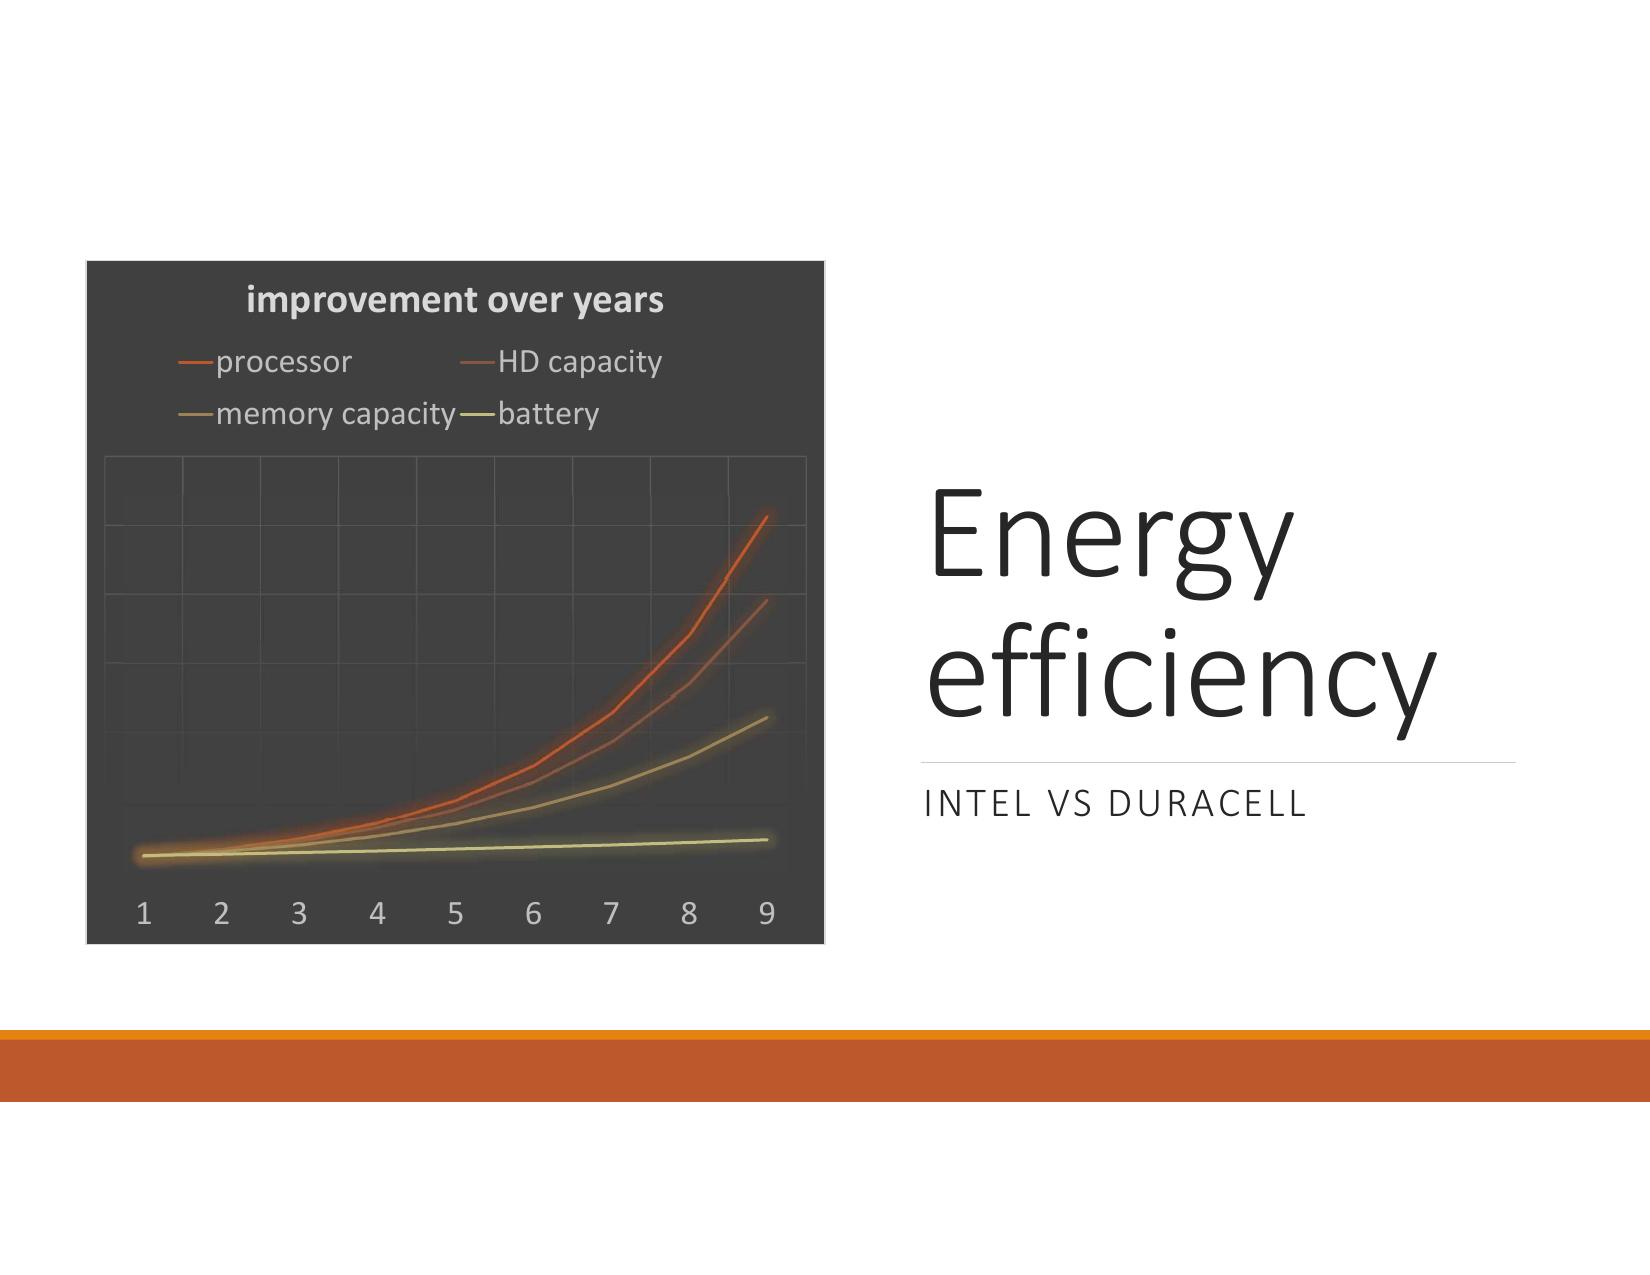
\includegraphics[keepaspectratio]{images/lezione-14-iot-design-img-01.jpg}}
\caption{Il confronto ``Intel vs Duracell'': le curve di processore, HD
e memoria crescono esponenzialmente nel tempo, mentre quella della
batteria rimane quasi orizzontale. Il gap energetico si allarga
progressivamente.}
\end{figure}

\subsection{Dove va l'energia: laptop vs
sensore}\label{dove-va-lenergia-laptop-vs-sensore}

\begin{figure}
\centering
\pandocbounded{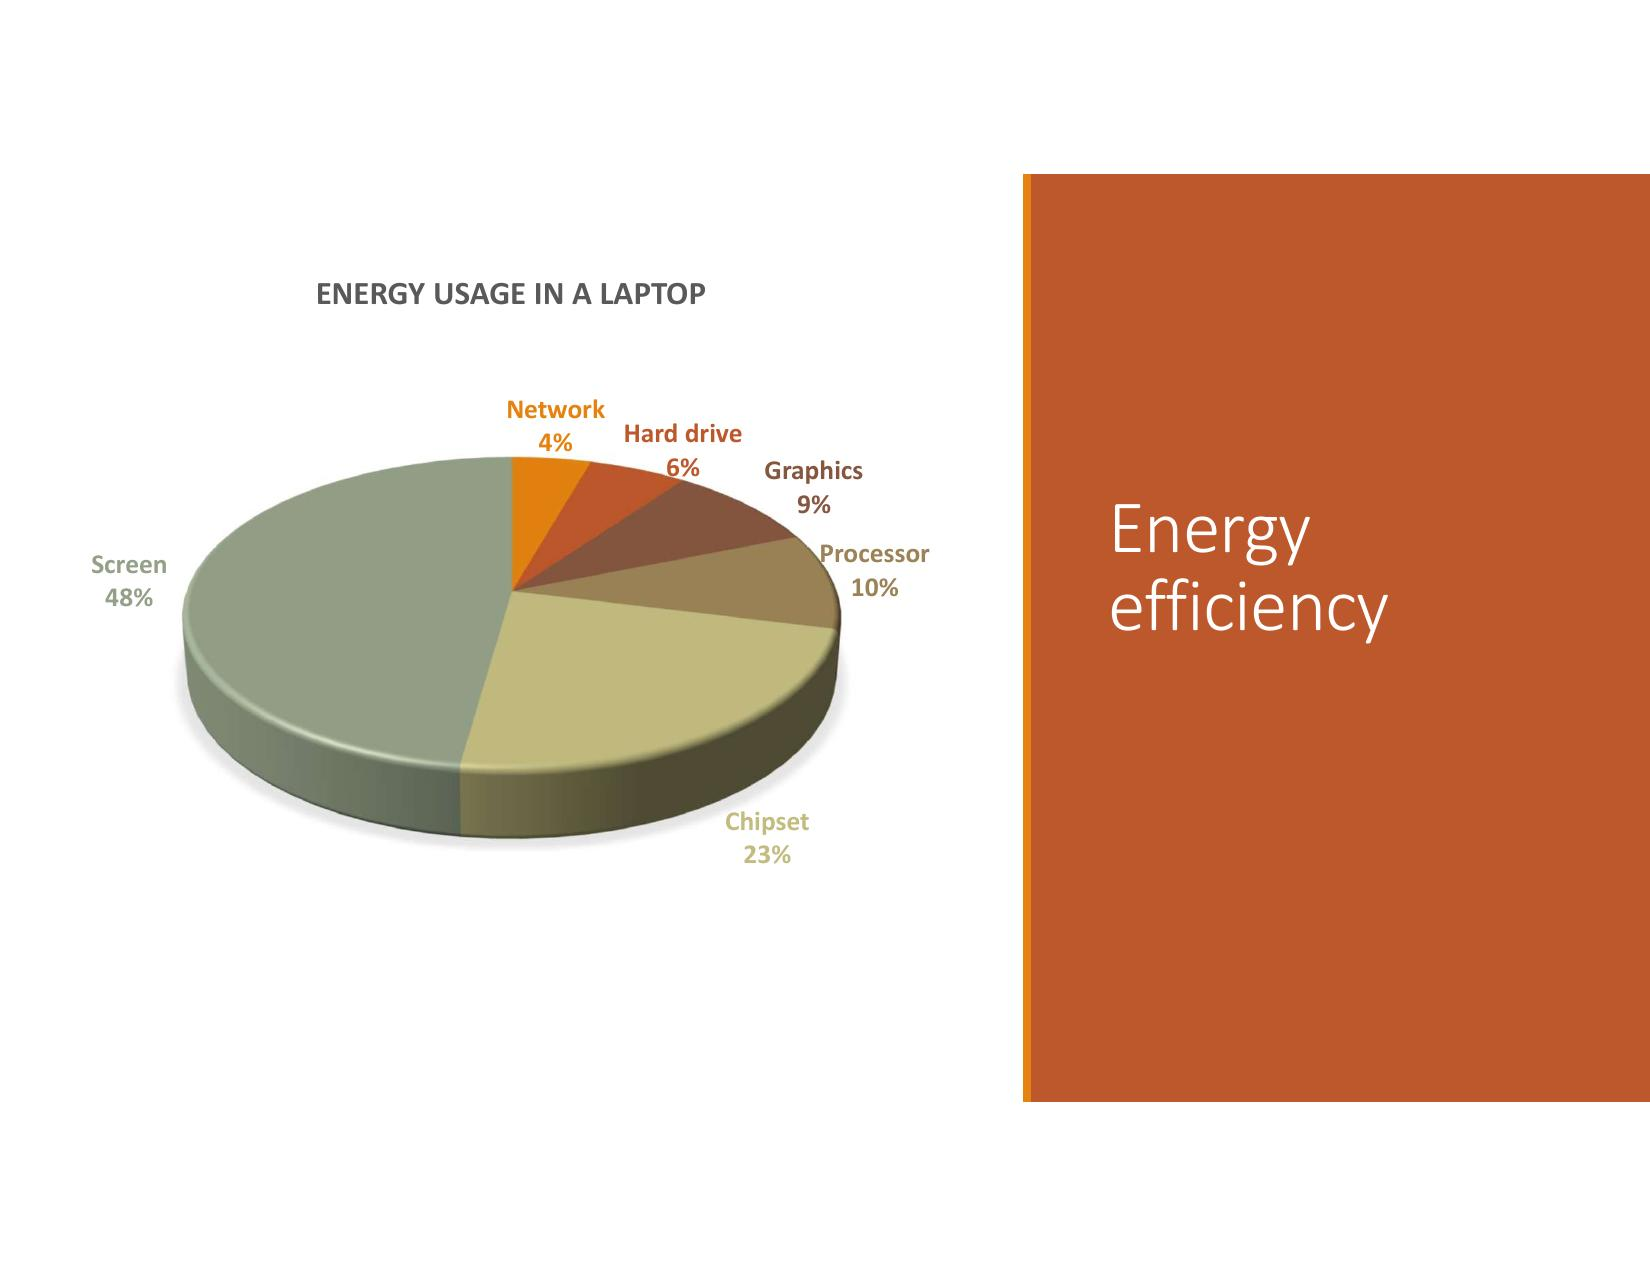
\includegraphics[keepaspectratio]{images/lezione-14-iot-design-img-02.jpg}}
\caption{Ripartizione del consumo in un laptop: lo schermo domina con il
48\%.}
\end{figure}

\begin{figure}
\centering
\pandocbounded{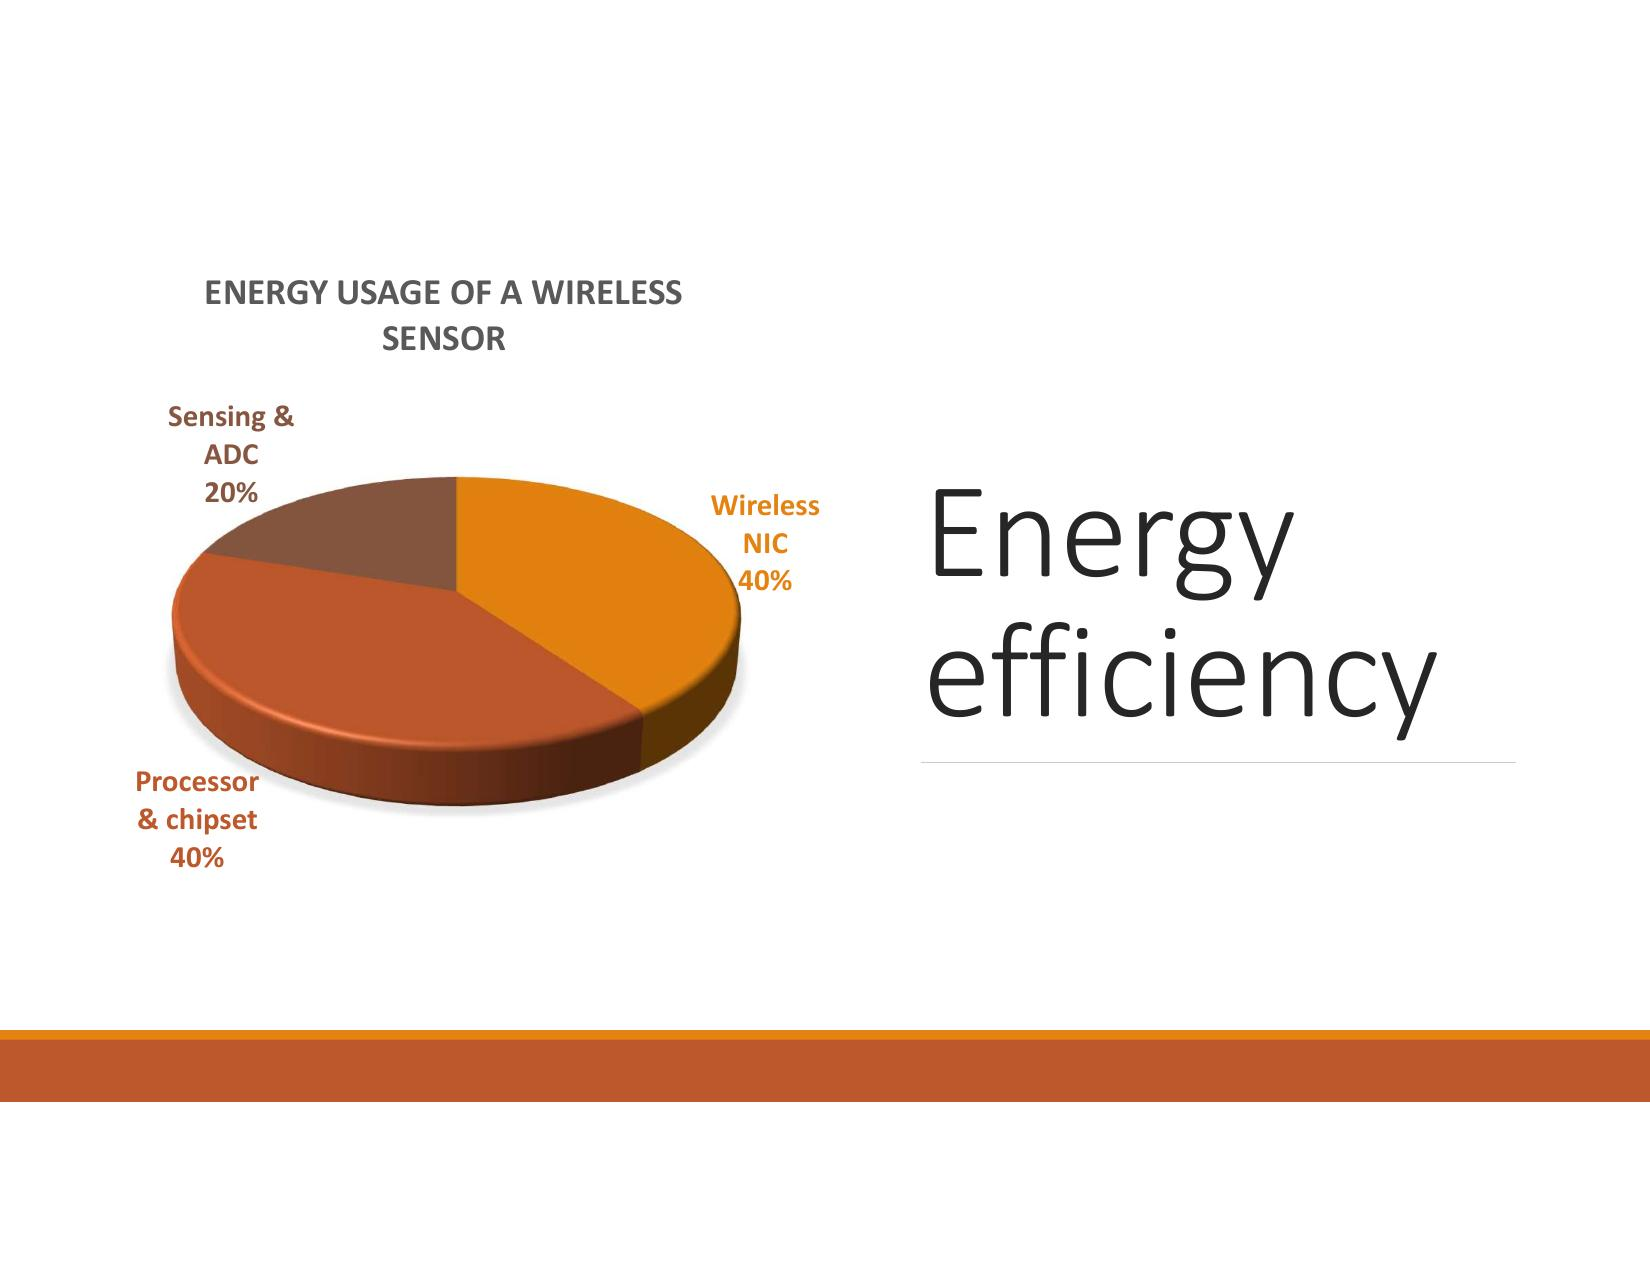
\includegraphics[keepaspectratio]{images/lezione-14-iot-design-img-03.jpg}}
\caption{Ripartizione del consumo in un sensore wireless: la radio (NIC)
e processore pesano il 40\% ciascuno, mentre il sensing pesa il 20\%.
Non essendoci schermo, la radio diventa il componente critico.}
\end{figure}

\textbf{Consumi della radio:} - Sleep mode: \textasciitilde10 mA -
\textbf{Listen mode (in ascolto): \textasciitilde180 mA} - Receive mode:
\textasciitilde200 mA - Transmit mode: \textasciitilde280 mA

\begin{calloutwarning}{Radio accesa = energia sprecata}

Il consumo in modalità listen è paragonabile a quello in ricezione, e
ordini di grandezza superiore allo sleep. La radio deve essere spenta il
più possibile. Anche tenere la radio accesa e in attesa è proibitivo.

\end{calloutwarning}

\subsection{Duty Cycle}\label{duty-cycle}

\begin{calloutdefinition}{Duty Cycle (DC)}

Il duty cycle è la frazione di un periodo in cui il sistema (o un suo
componente) è attivo: \(DC = \frac{t_{attivo}}{T_{periodo}}\).

\end{calloutdefinition}

Applicare duty cycle aggressivi (es. 1-5\%) è la leva principale per
estendere la vita della batteria, disattivando hardware non necessario
in ogni porzione di firmware. Il consumo medio è dettato da
\(E = dc \cdot C_{active} + (1 - dc) \cdot C_{idle}\).

\begin{figure}
\centering
\pandocbounded{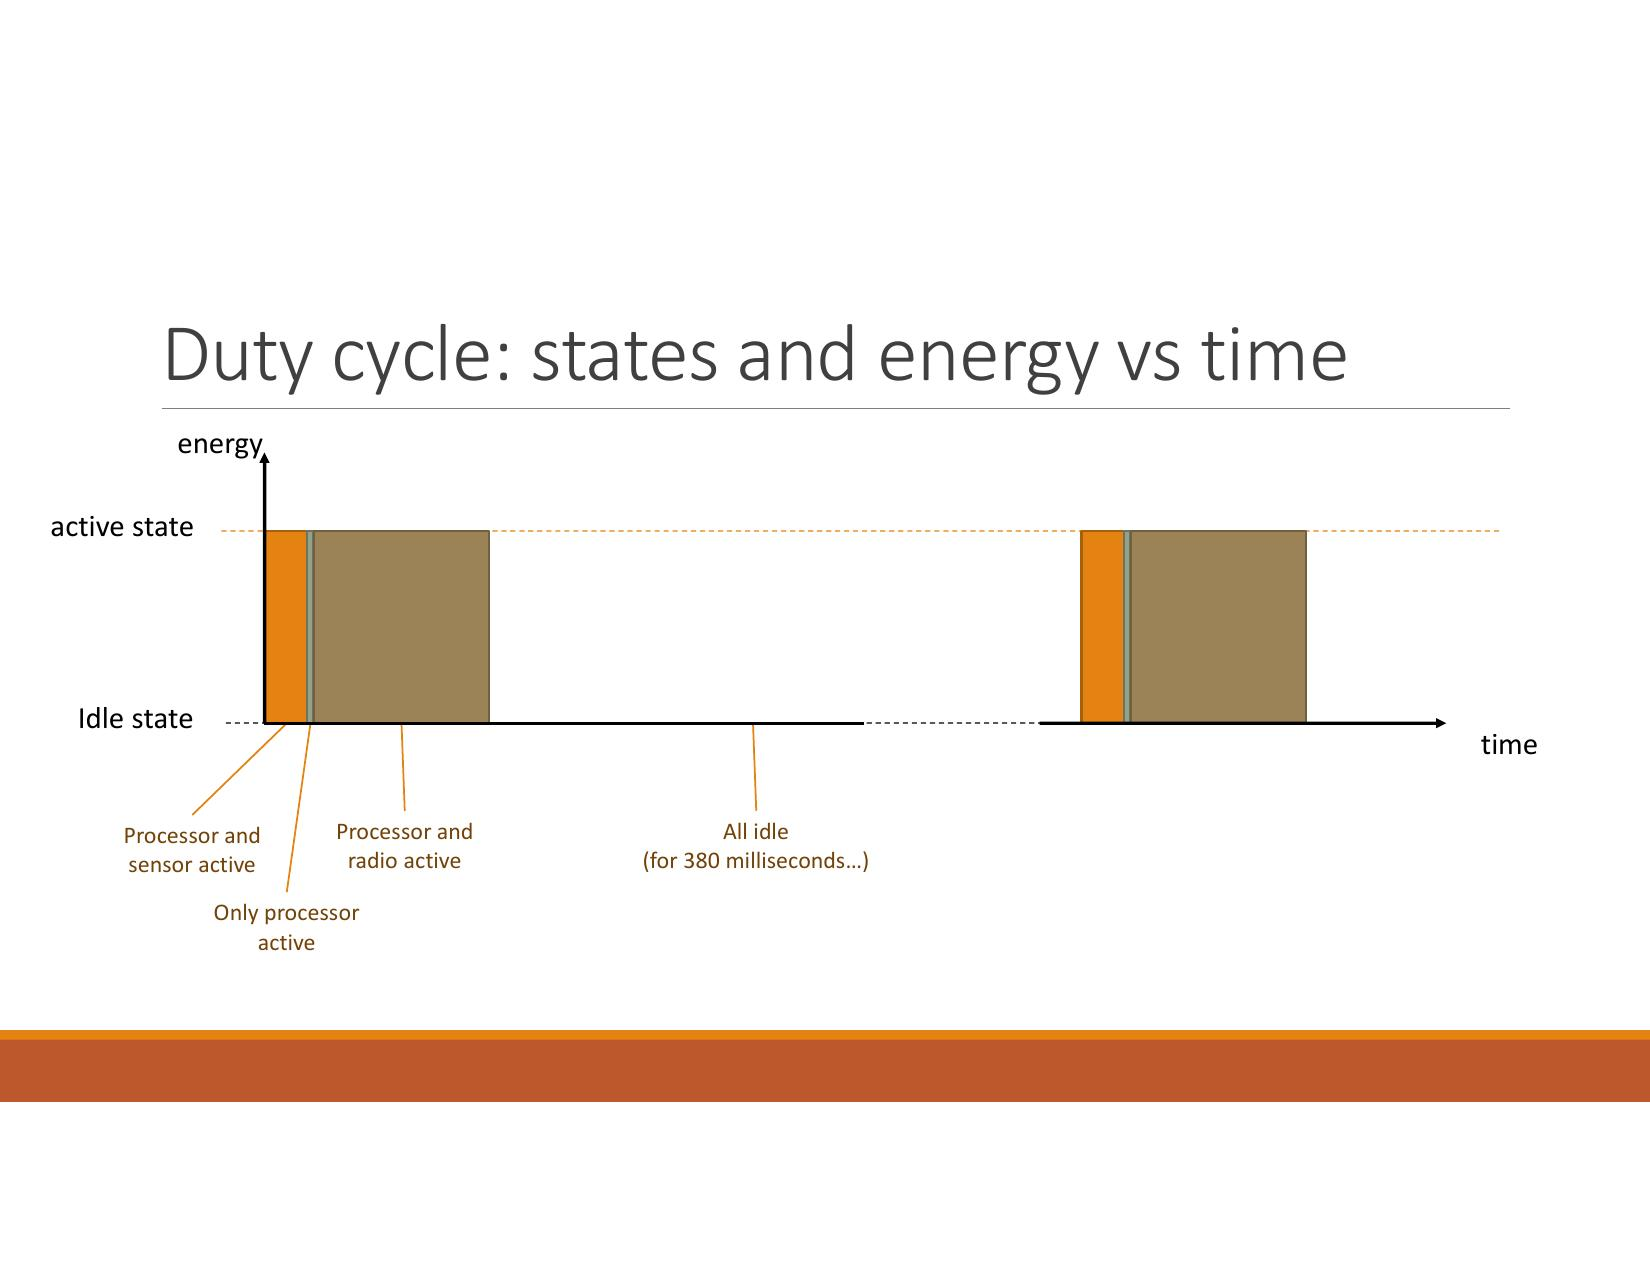
\includegraphics[keepaspectratio]{images/lezione-14-iot-design-img-04.jpg}}
\caption{Diagramma stati/energia vs tempo per un codice di esempio con
turnOn e turnOff dei componenti. Il lungo periodo di idle (380 ms su 400
ms) abbassa drasticamente il consumo medio.}
\end{figure}

\begin{figure}
\centering
\pandocbounded{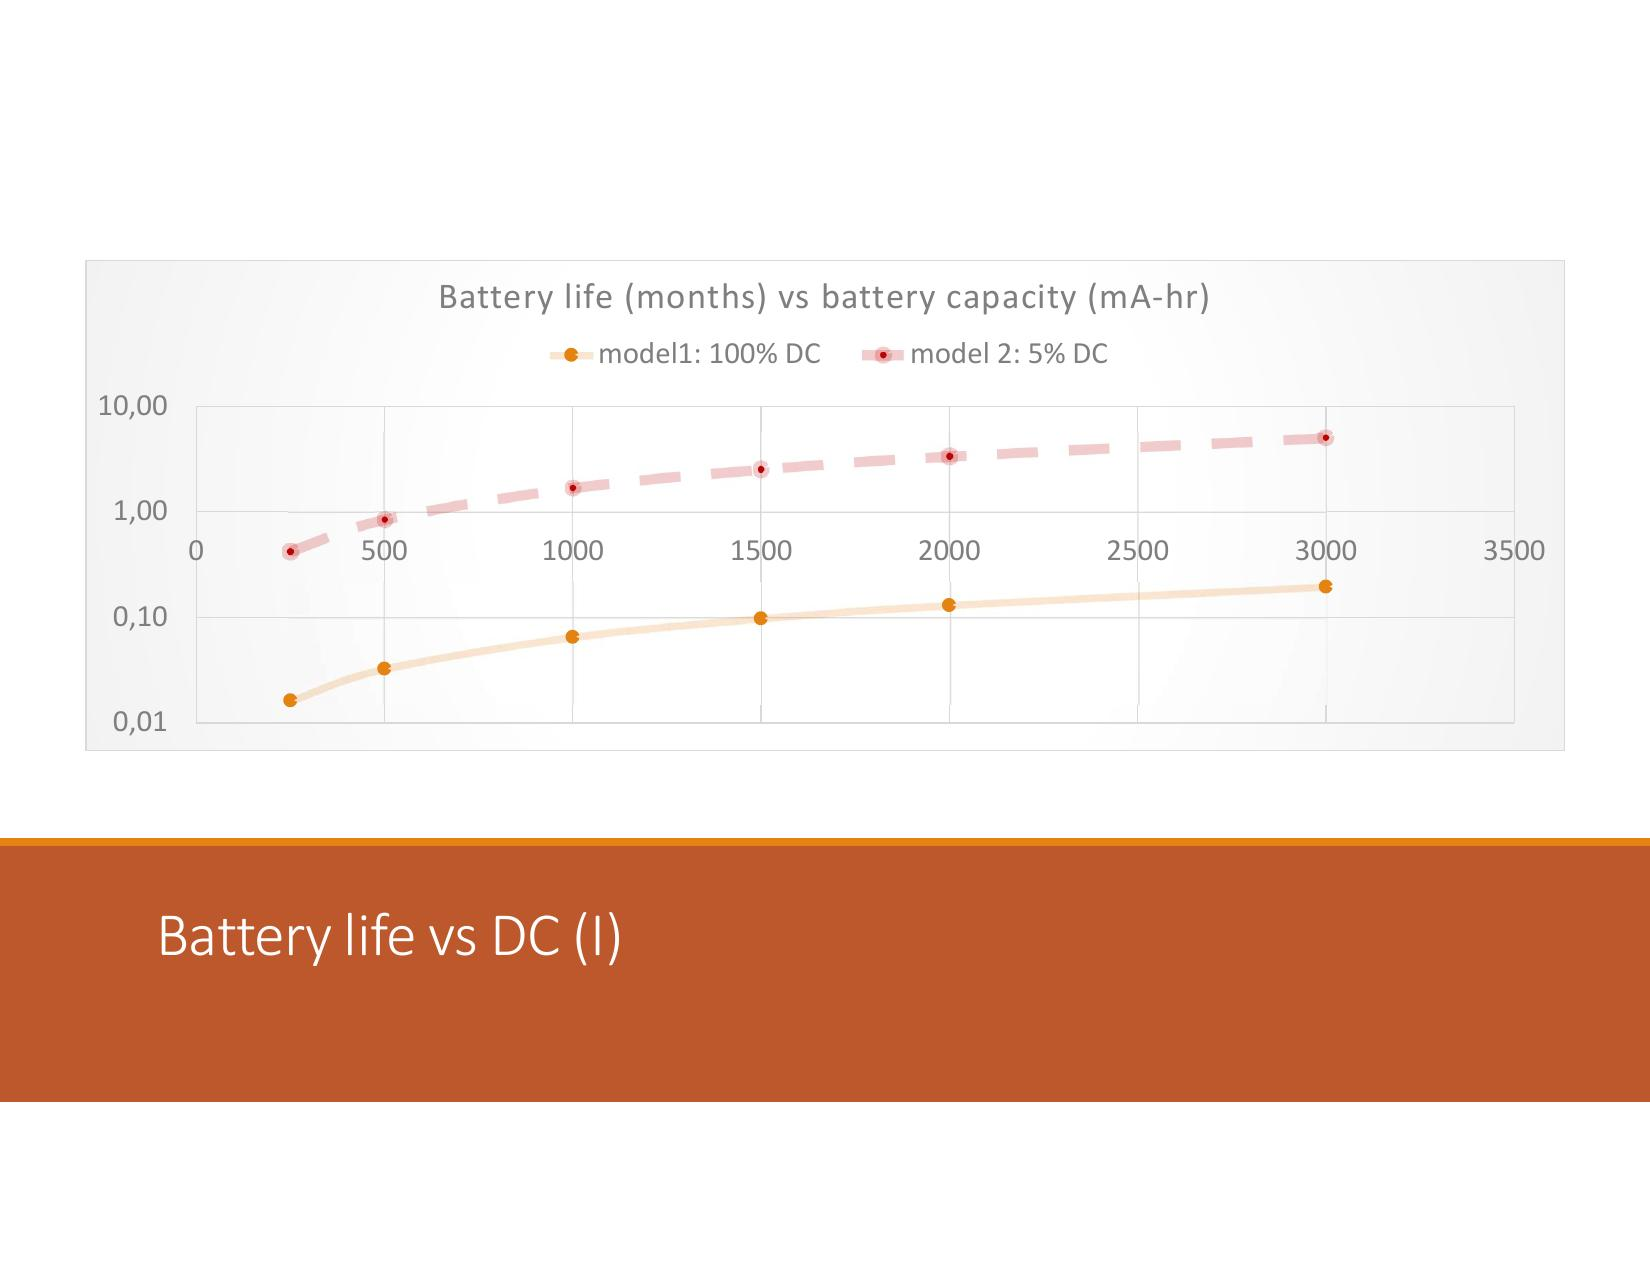
\includegraphics[keepaspectratio]{images/lezione-14-iot-design-img-05.jpg}}
\caption{Vita della batteria vs capacità. Un modello con DC al 5\% ha
una vita 10-15 volte superiore a uno con DC al 100\%.}
\end{figure}

\begin{figure}
\centering
\pandocbounded{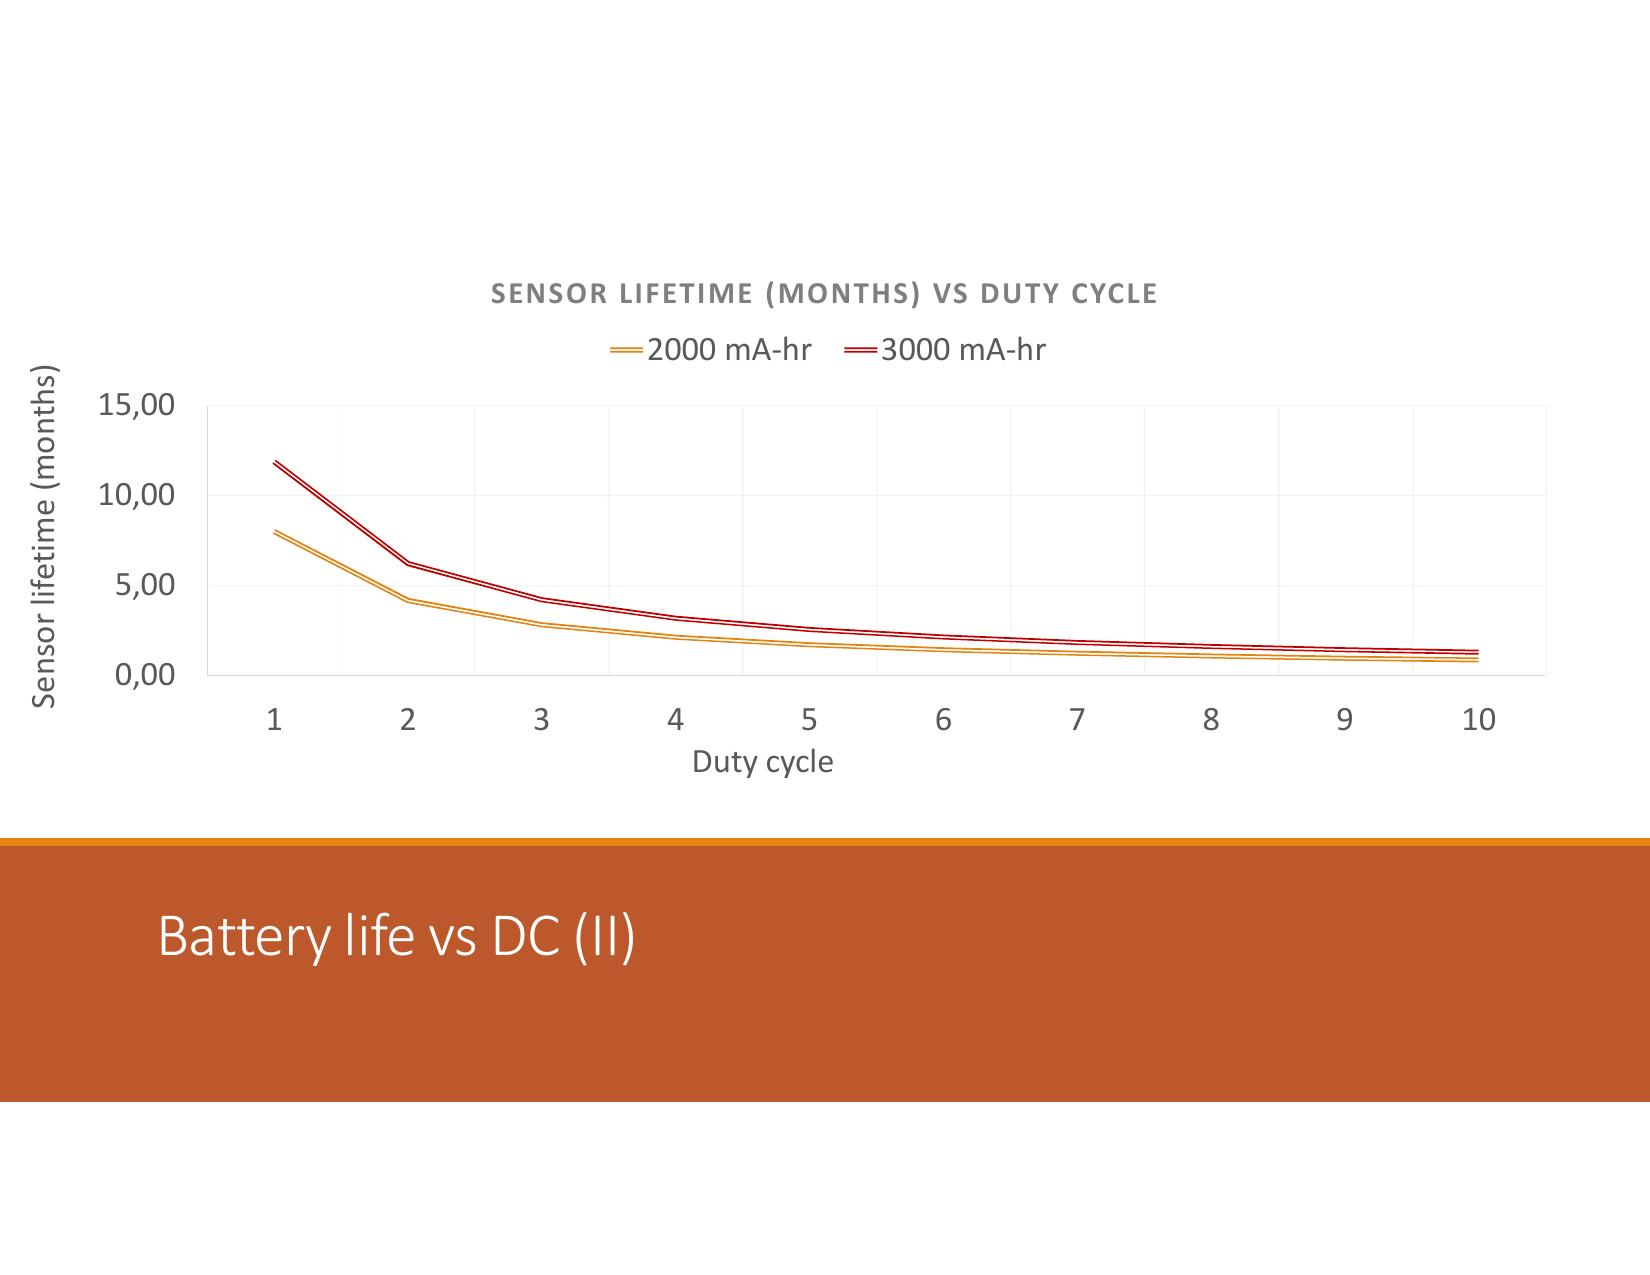
\includegraphics[keepaspectratio]{images/lezione-14-iot-design-img-06.jpg}}
\caption{Vita del sensore vs duty cycle: la curva scende molto
rapidamente. Ridurre il DC da 3\% a 1\% genera incrementi molto più
incisivi rispetto all'aumentare la batteria da 2000 a 3000 mAh.}
\end{figure}

Spegnere la radio tuttavia è una \textbf{decisione globale} che richiede
protocolli MAC IoT specializzati per permettere la comunicazione
sincrona e il risveglio coordinato.

\begin{figure}
\centering
\pandocbounded{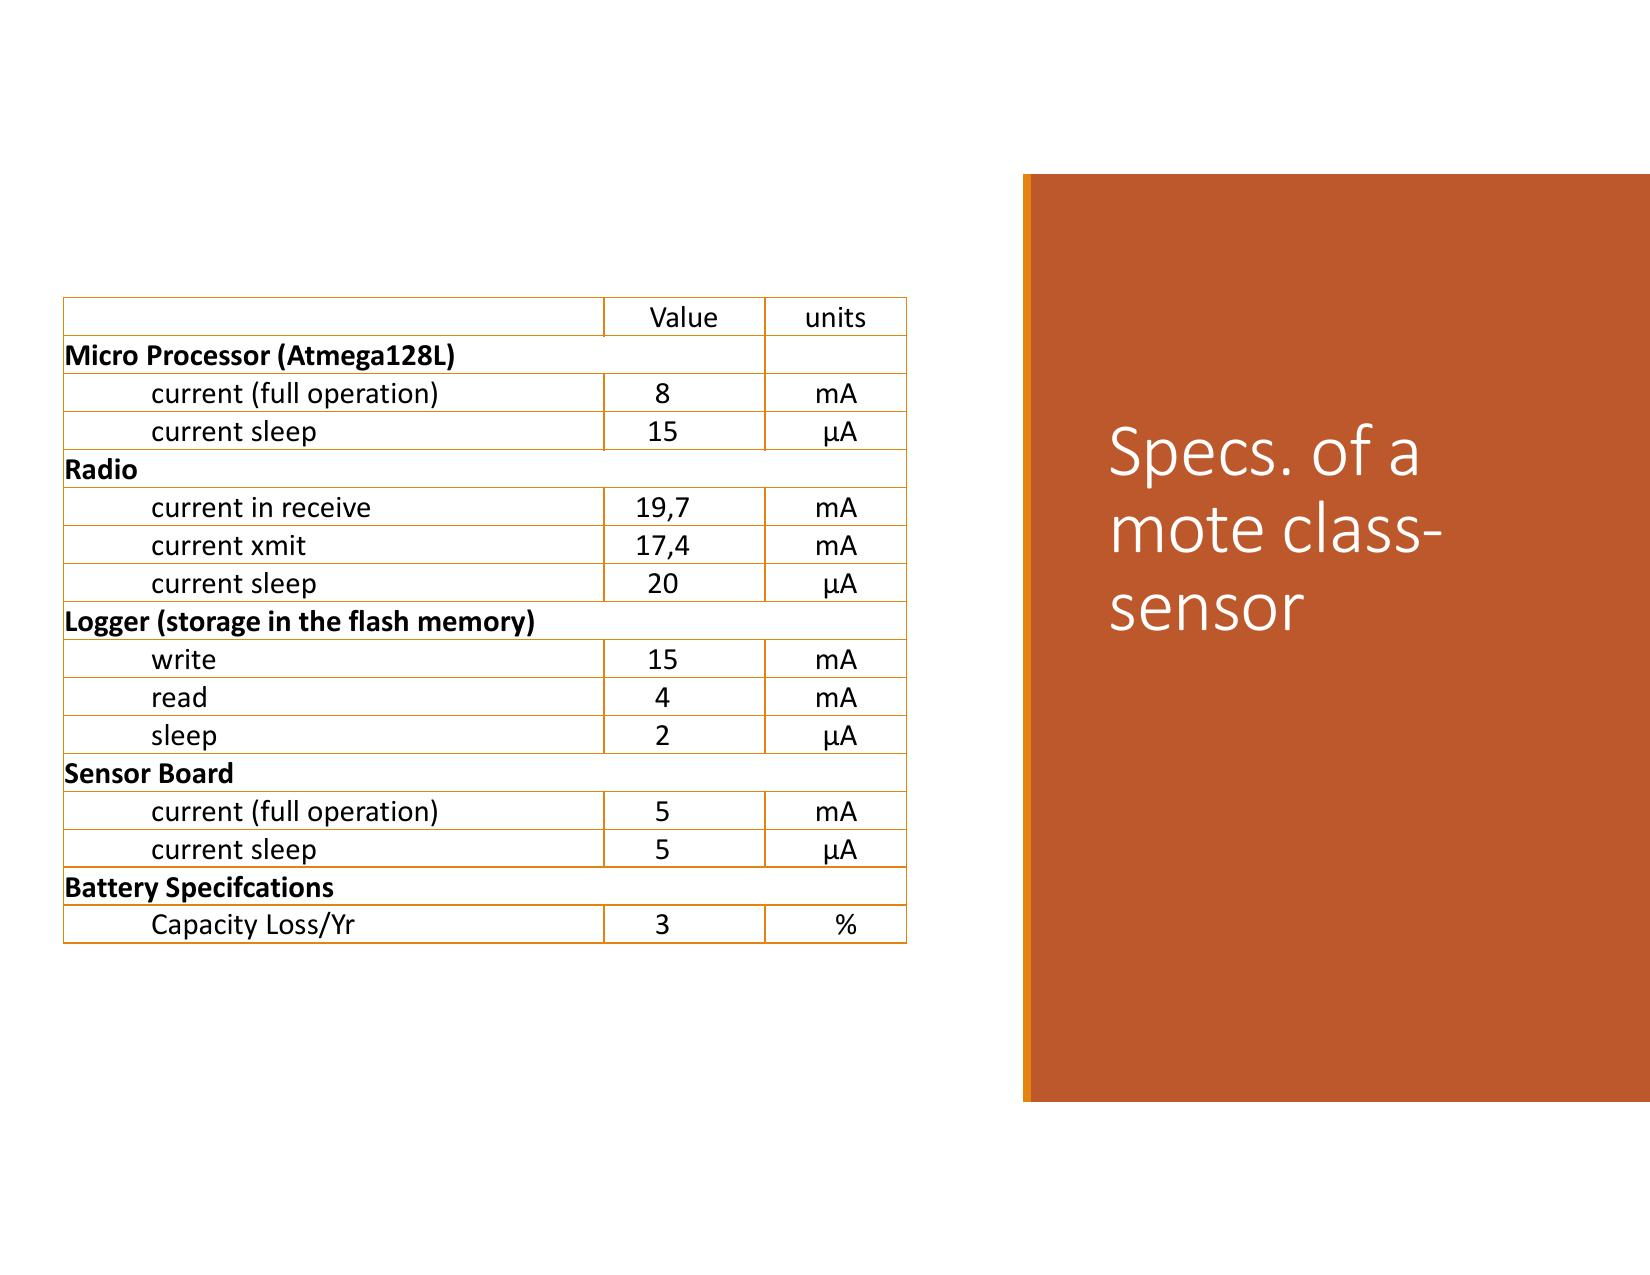
\includegraphics[keepaspectratio]{images/lezione-14-iot-design-img-07.jpg}}
\caption{Specifiche hardware complete di una Mote-class sensor.}
\end{figure}

\begin{figure}
\centering
\pandocbounded{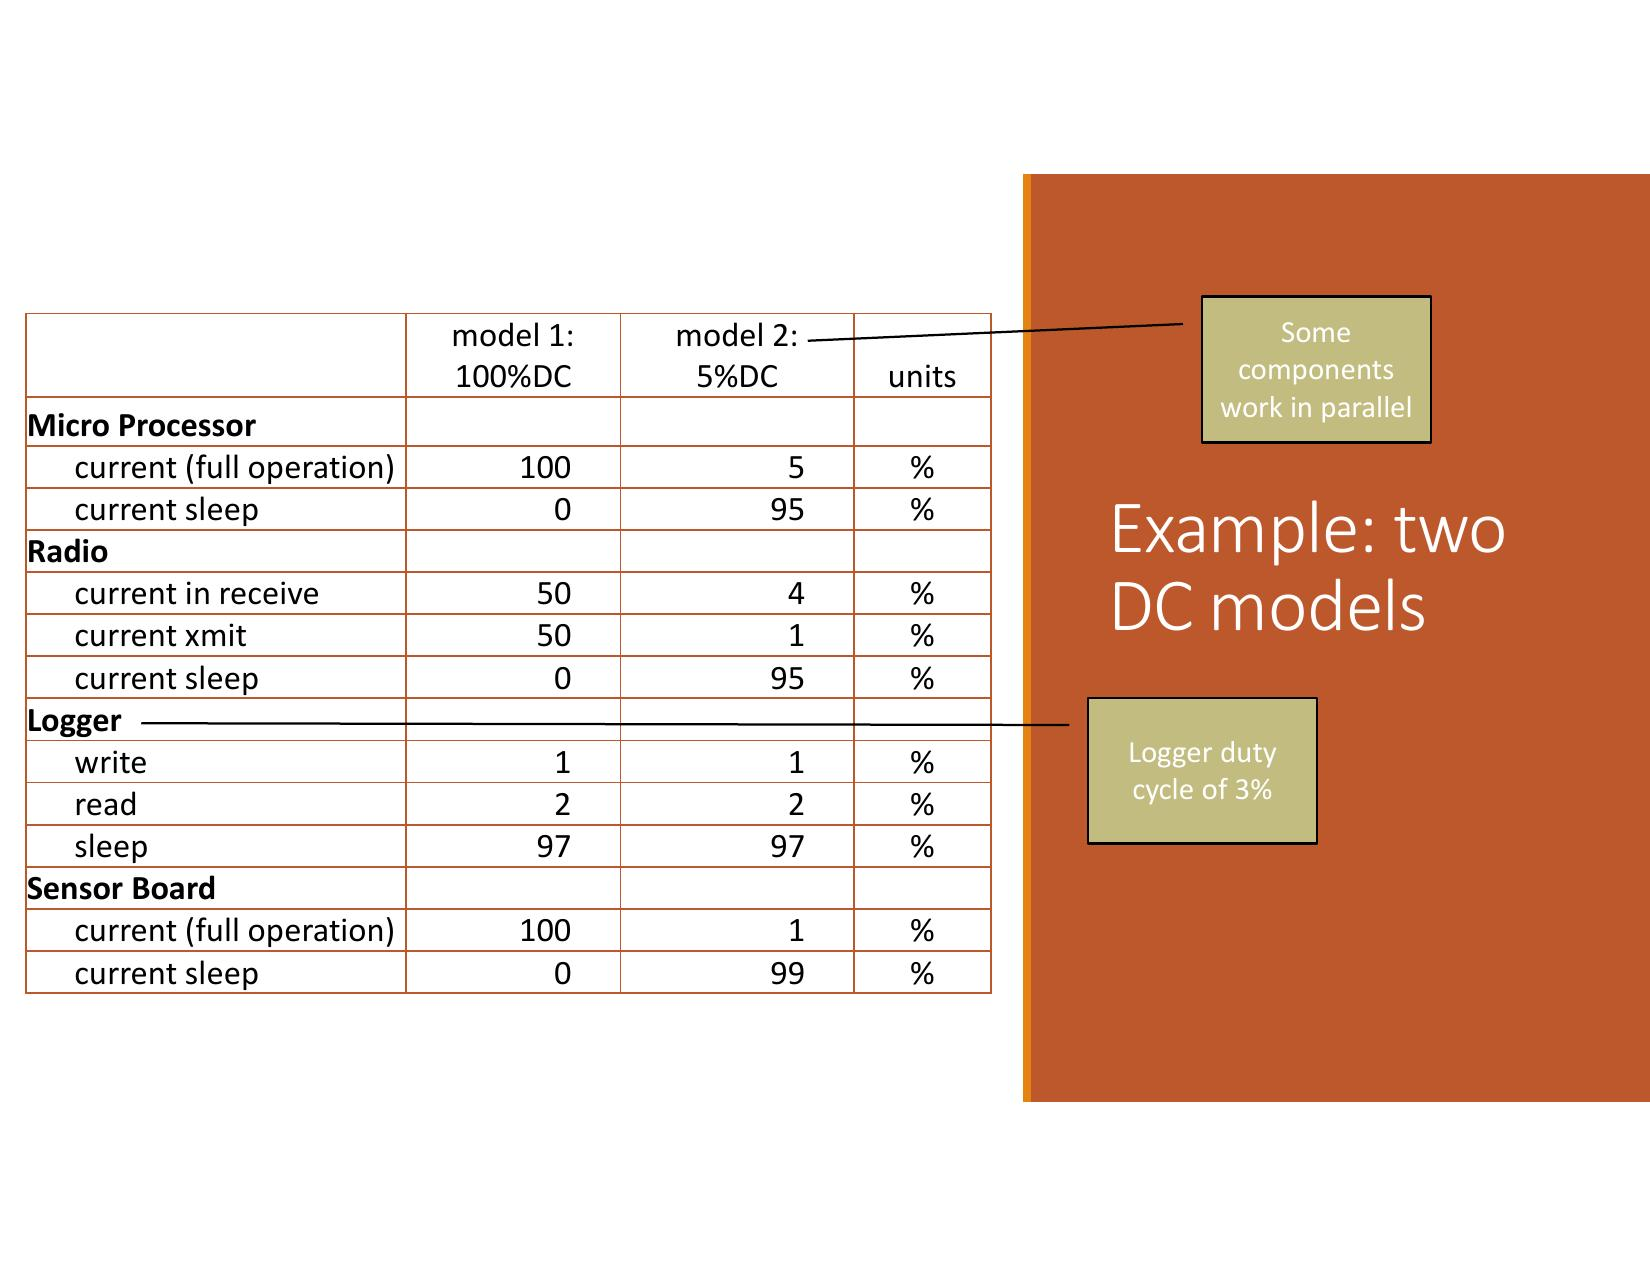
\includegraphics[keepaspectratio]{images/lezione-14-iot-design-img-08.jpg}}
\caption{Tabella di confronto tra il modello DC 100\% e il modello DC
5\%.}
\end{figure}

\begin{figure}
\centering
\pandocbounded{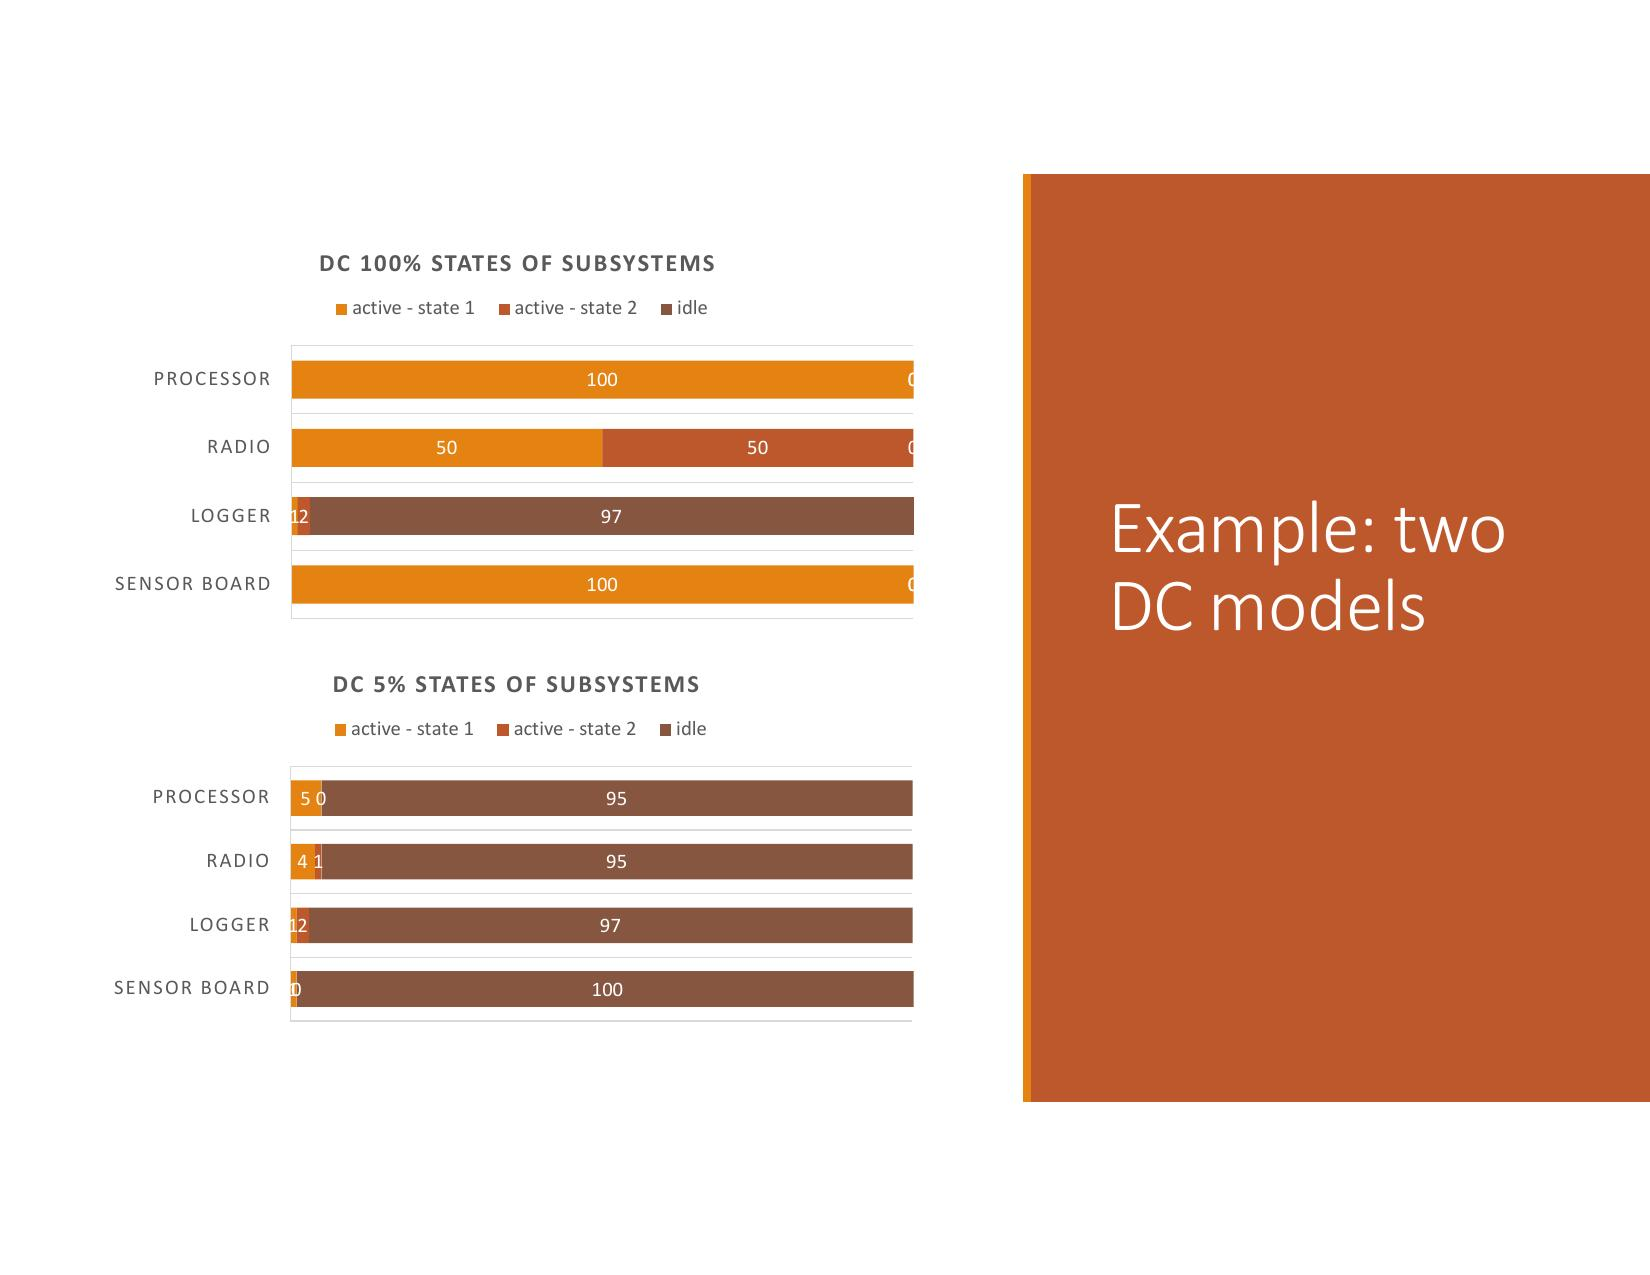
\includegraphics[keepaspectratio]{images/lezione-14-iot-design-img-09.jpg}}
\caption{Rappresentazione grafica degli stati. DC 5\% trascorre quasi
tutto il tempo idle.}
\end{figure}

\begin{figure}
\centering
\pandocbounded{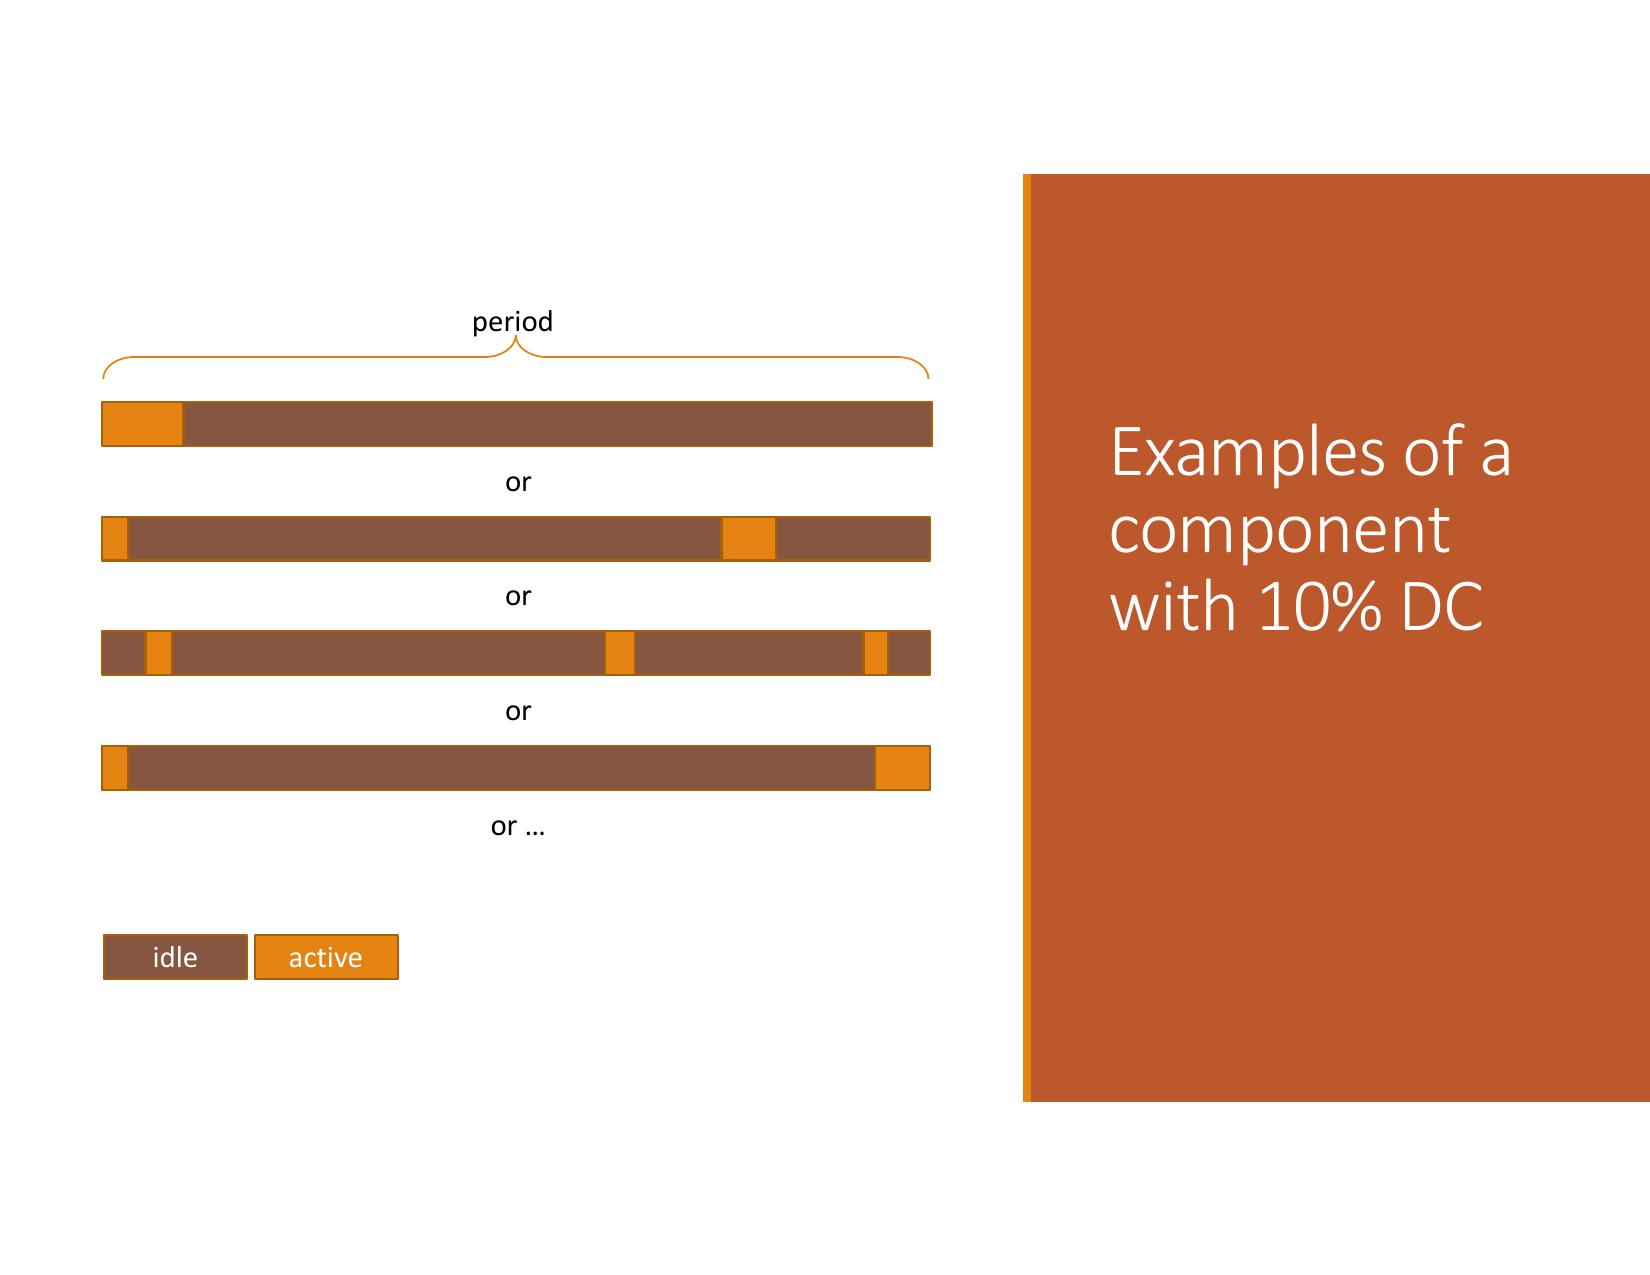
\includegraphics[keepaspectratio]{images/lezione-14-iot-design-img-10.jpg}}
\caption{Il duty cycle non specifica la posizione dell'attività nel
tempo; questo offre flessibilità per la sincronizzazione MAC tra nodi.}
\end{figure}

\begin{center}\rule{0.5\linewidth}{0.5pt}\end{center}

\section{8. Case Study: Biologging e Activity
Recognition}\label{case-study-biologging-e-activity-recognition}

Il biologging rappresenta uno dei casi d'uso più concreti dell'IoT nel
mondo naturale. Il progetto \textbf{Tortoise@} automatizza il
rilevamento delle attività di nidificazione delle tartarughe con ML
embedded su dispositivi a bassa potenza.

\begin{calloutdefinition}{Biotelemetria vs Bio-logging}

\textbf{Biotelemetria}: i dati raccolti vengono trasmessi in tempo
reale. \textbf{Bio-logging}: i dati vengono memorizzati internamente per
recupero fisico, ed eventualmente trasmessi solo quando richiesto.

\end{calloutdefinition}

\subsection{Pipeline del Biologging e On-Board
Intelligence}\label{pipeline-del-biologging-e-on-board-intelligence}

Il monitoraggio con accelerometri e GPS continui esaurirebbe in fretta
le batterie. \textbf{Approccio innovativo}: spostare l'elaborazione
(Machine Learning) \textbf{on-board}, analizzare in locale, e
trasmettere via radio \textbf{solo il risultato semantico}.

\begin{figure}
\centering
\pandocbounded{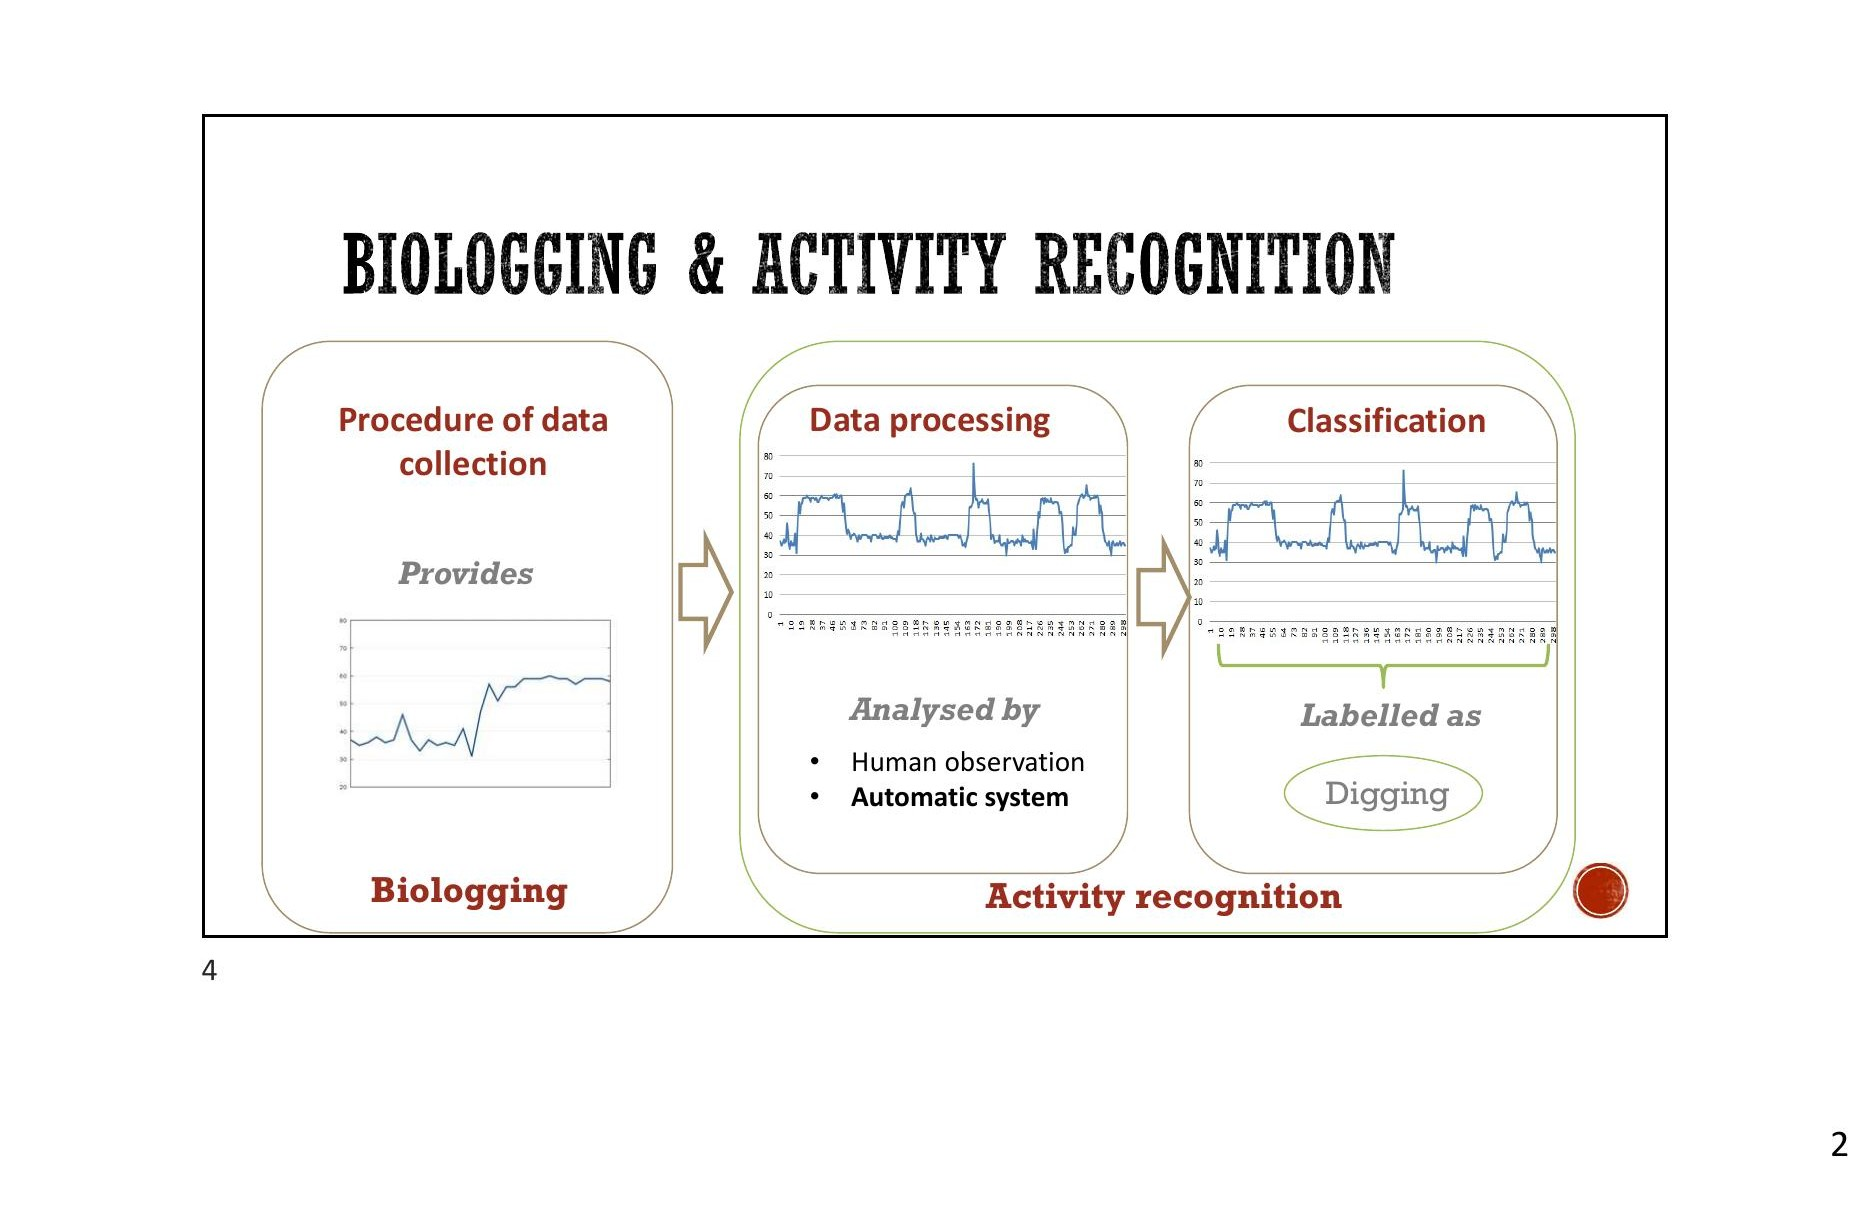
\includegraphics[keepaspectratio]{images/lezione-19-caso-studio-tartarughe-img-01.jpg}}
\caption{Il flusso completo del biologging.}
\end{figure}

\begin{figure}
\centering
\pandocbounded{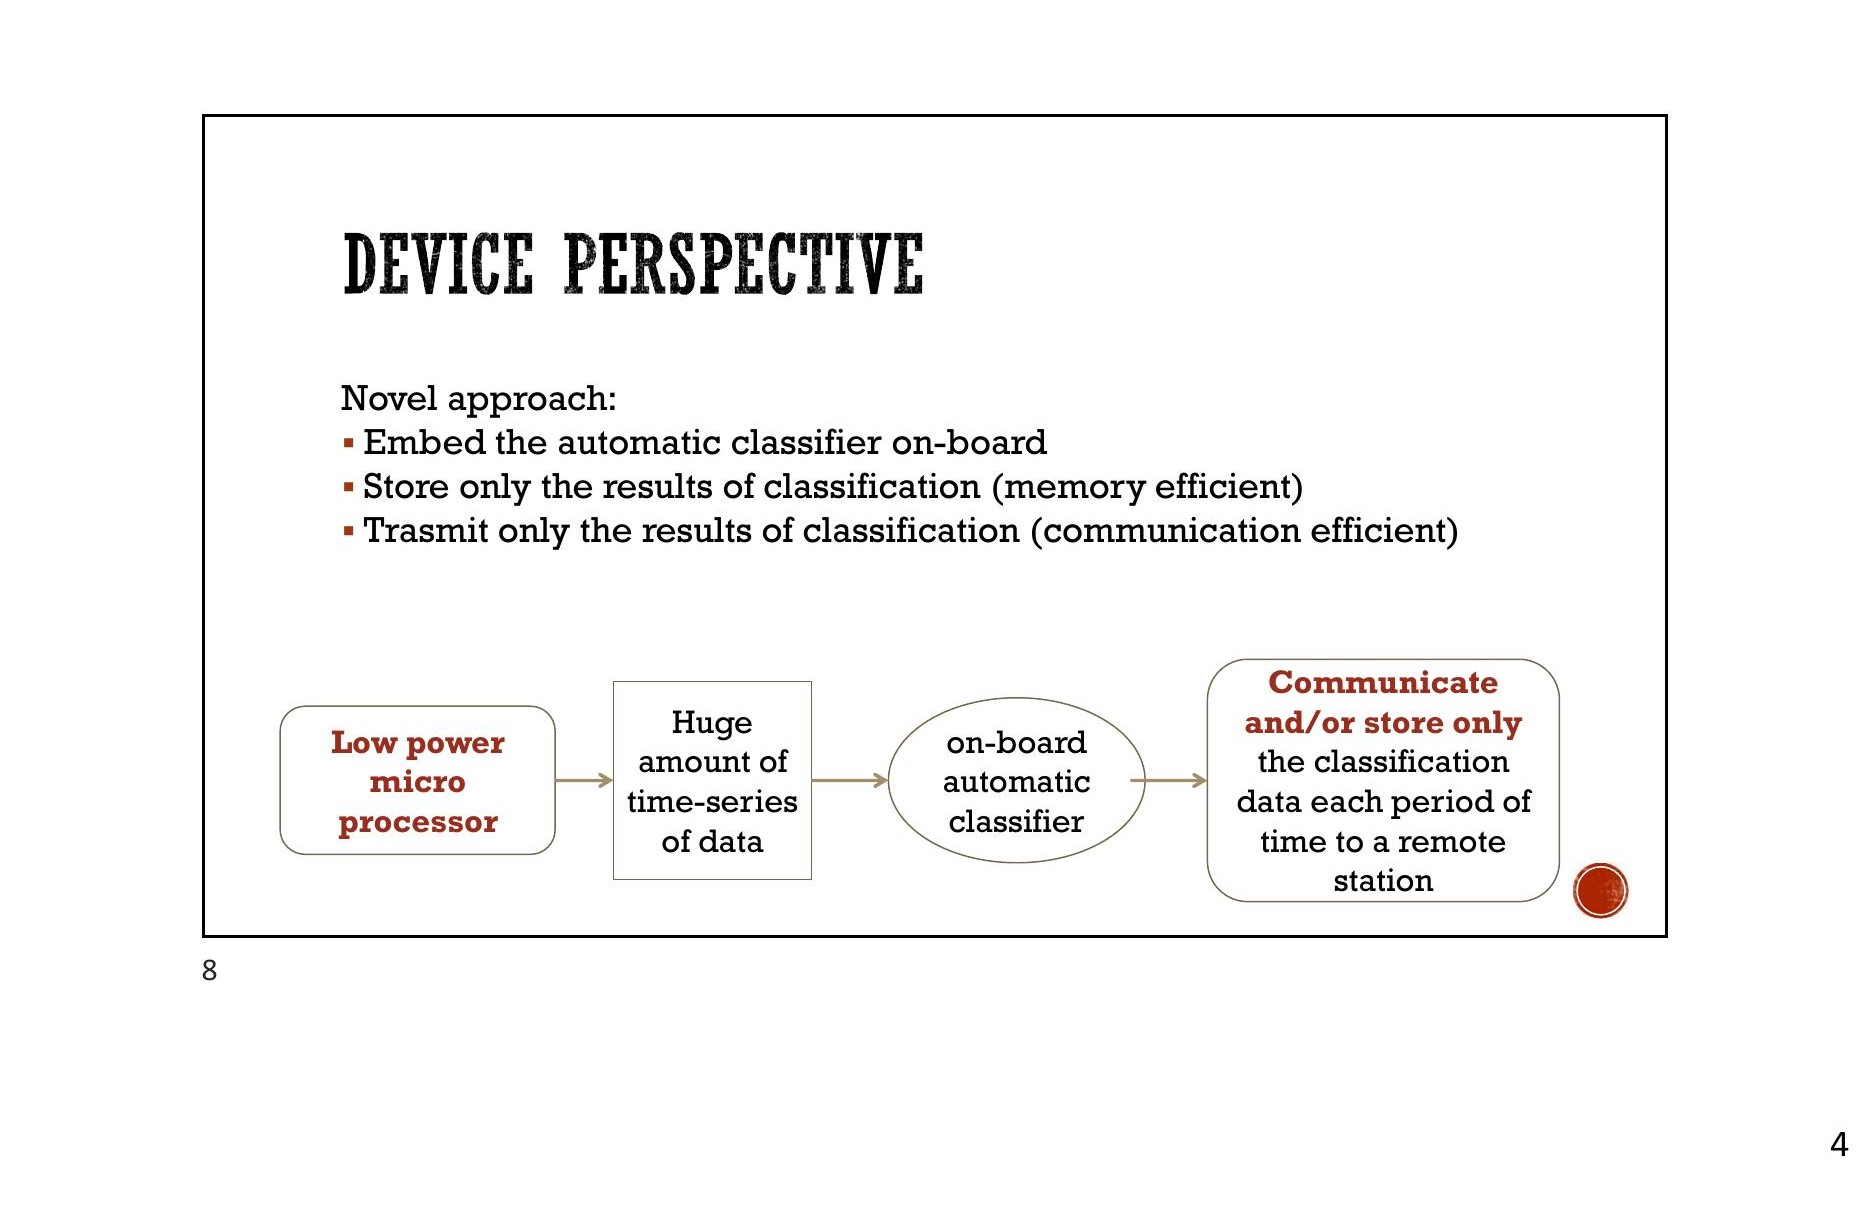
\includegraphics[keepaspectratio]{images/lezione-19-caso-studio-tartarughe-img-02.jpg}}
\caption{L'elaborazione e memorizzazione solo dei risultati riduce
drasticamente traffico radio e consumi.}
\end{figure}

\subsection{Il progetto Tortoise@}\label{il-progetto-tortoise}

Il sistema serve a ritrovare i nidi deposti individuando il segnale
accelerometrico dello scavo: - Lo scavo produce un pattern
caratteristico imparabile. - Le tartarughe nidificano in giorno in
luoghi caldi.

\begin{figure}
\centering
\pandocbounded{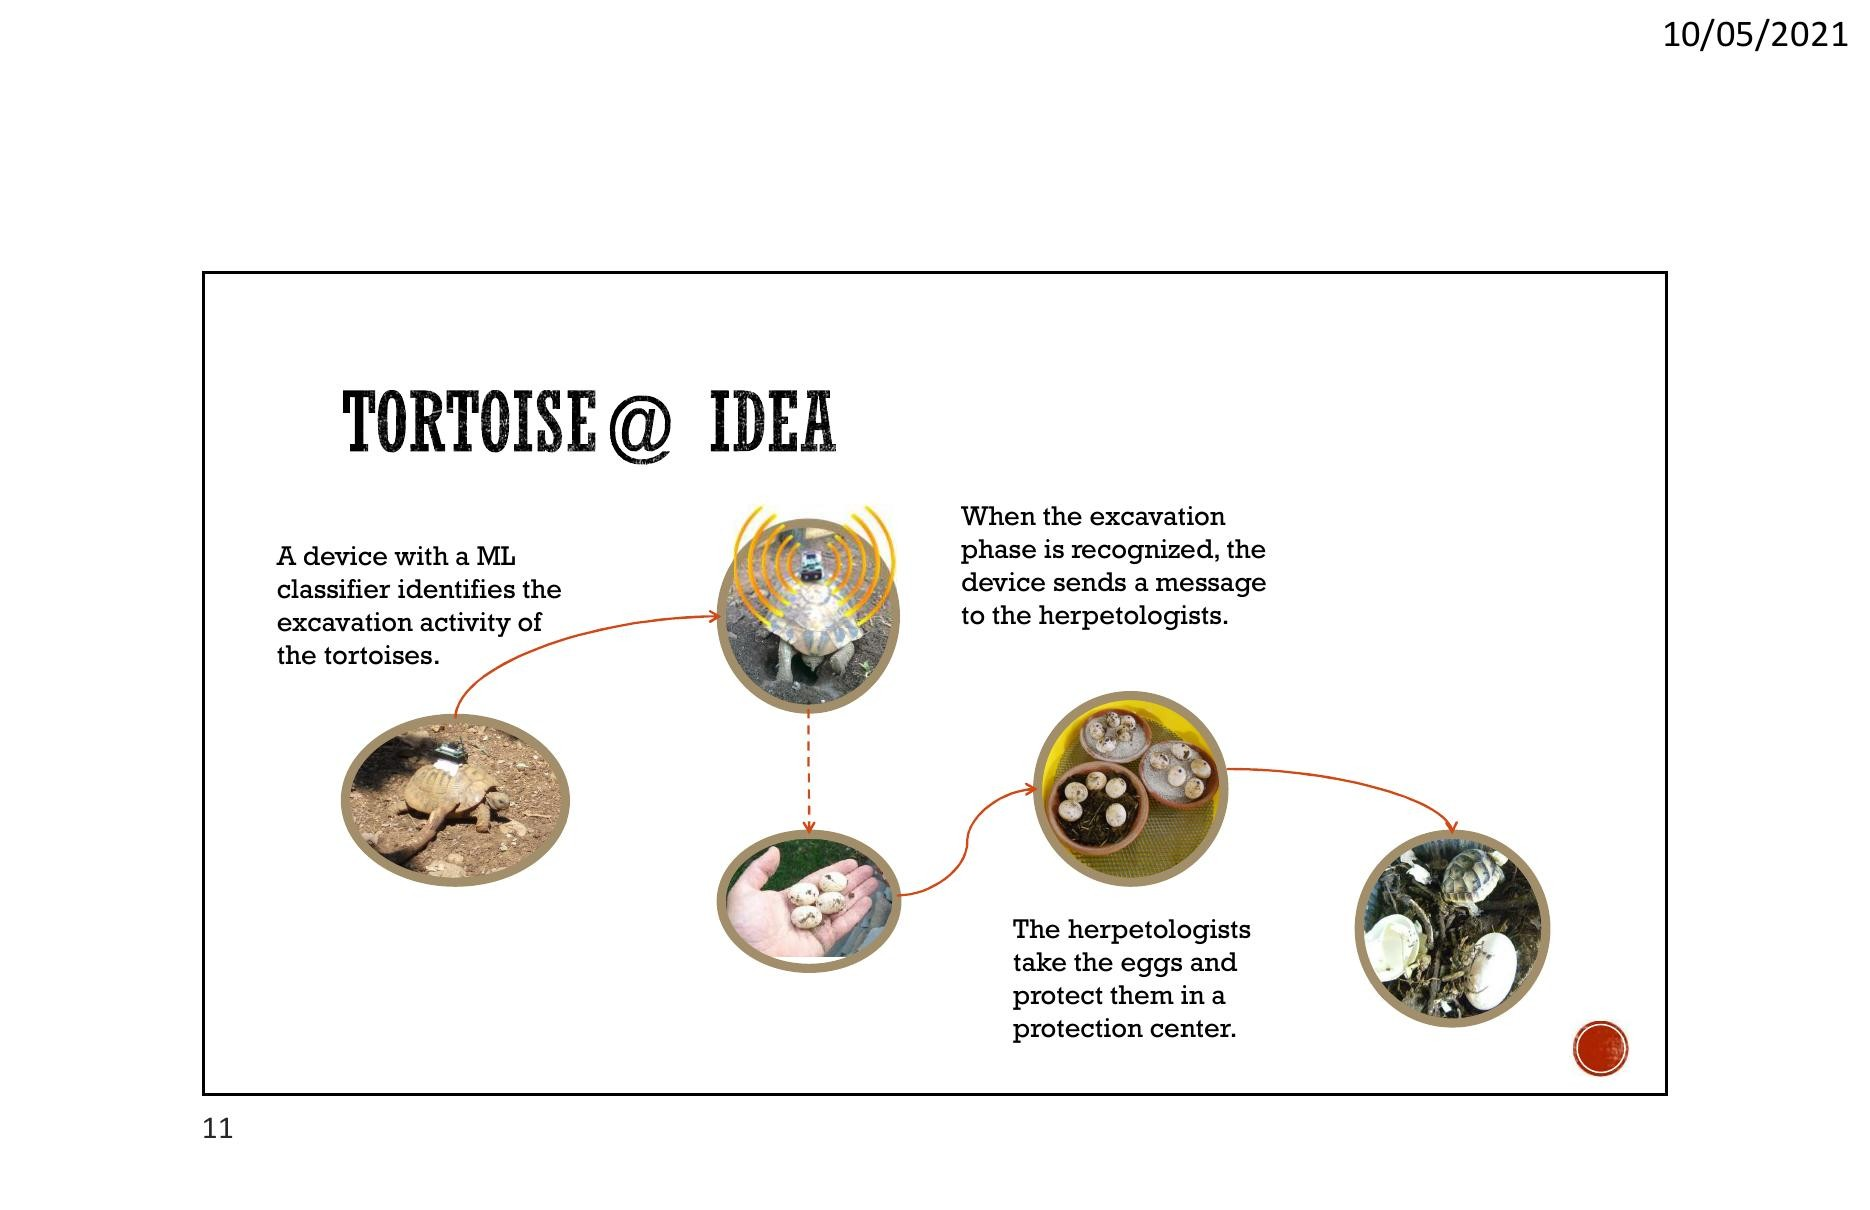
\includegraphics[keepaspectratio]{images/lezione-19-caso-studio-tartarughe-img-03.jpg}}
\caption{Il sistema invia notifiche GPS agli erpetologi appena riconosce
il nido.}
\end{figure}

\begin{figure}
\centering
\pandocbounded{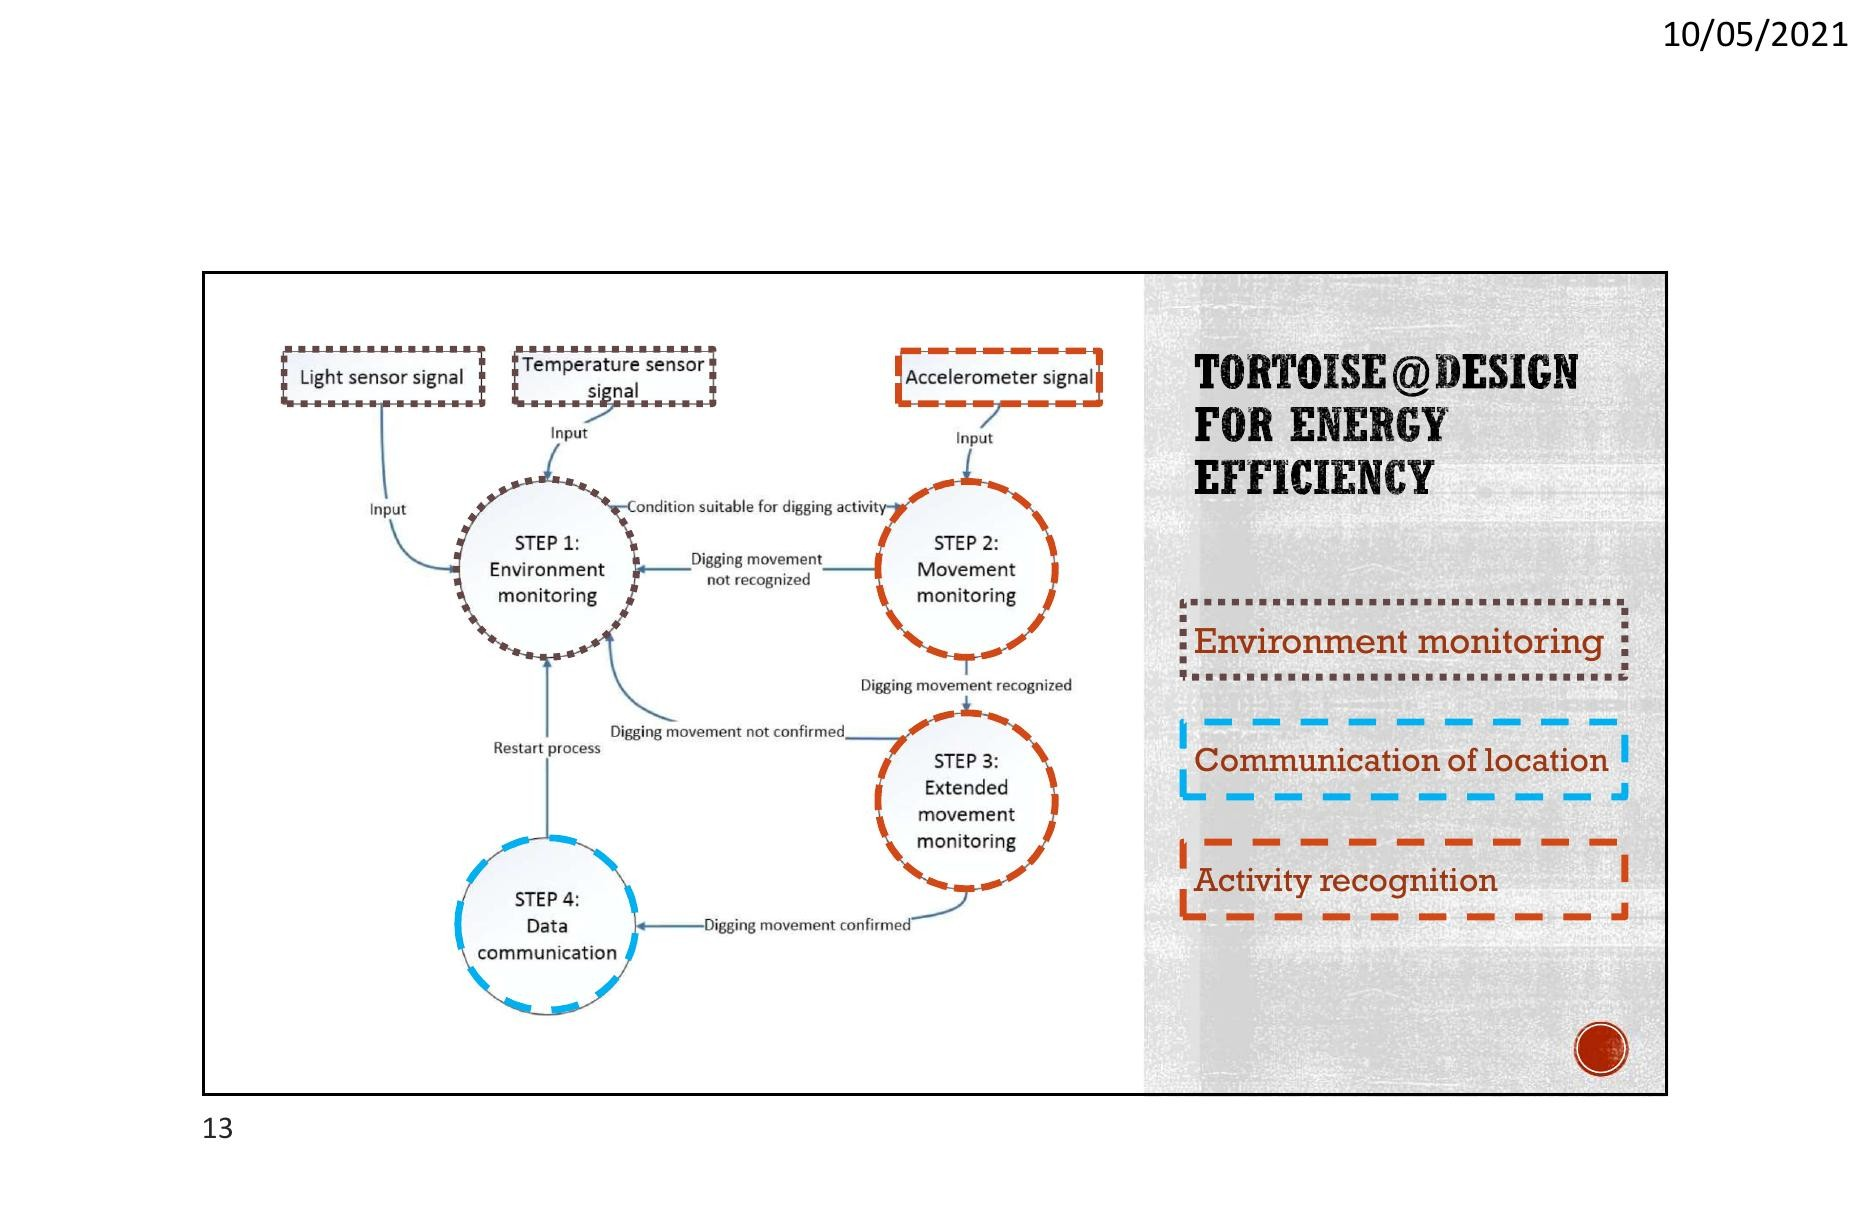
\includegraphics[keepaspectratio]{images/lezione-19-caso-studio-tartarughe-img-04.jpg}}
\caption{Macchina a stati finiti: usa sensori luce/temperatura molto
economici come ``gate'' per azionare i dispendiosi accelerometri solo
quando ha senso.}
\end{figure}

\subsection{Classificazione}\label{classificazione}

Sensori MicaZ a 1Hz su asse X, finestre asincrone e sincrone.
\pandocbounded{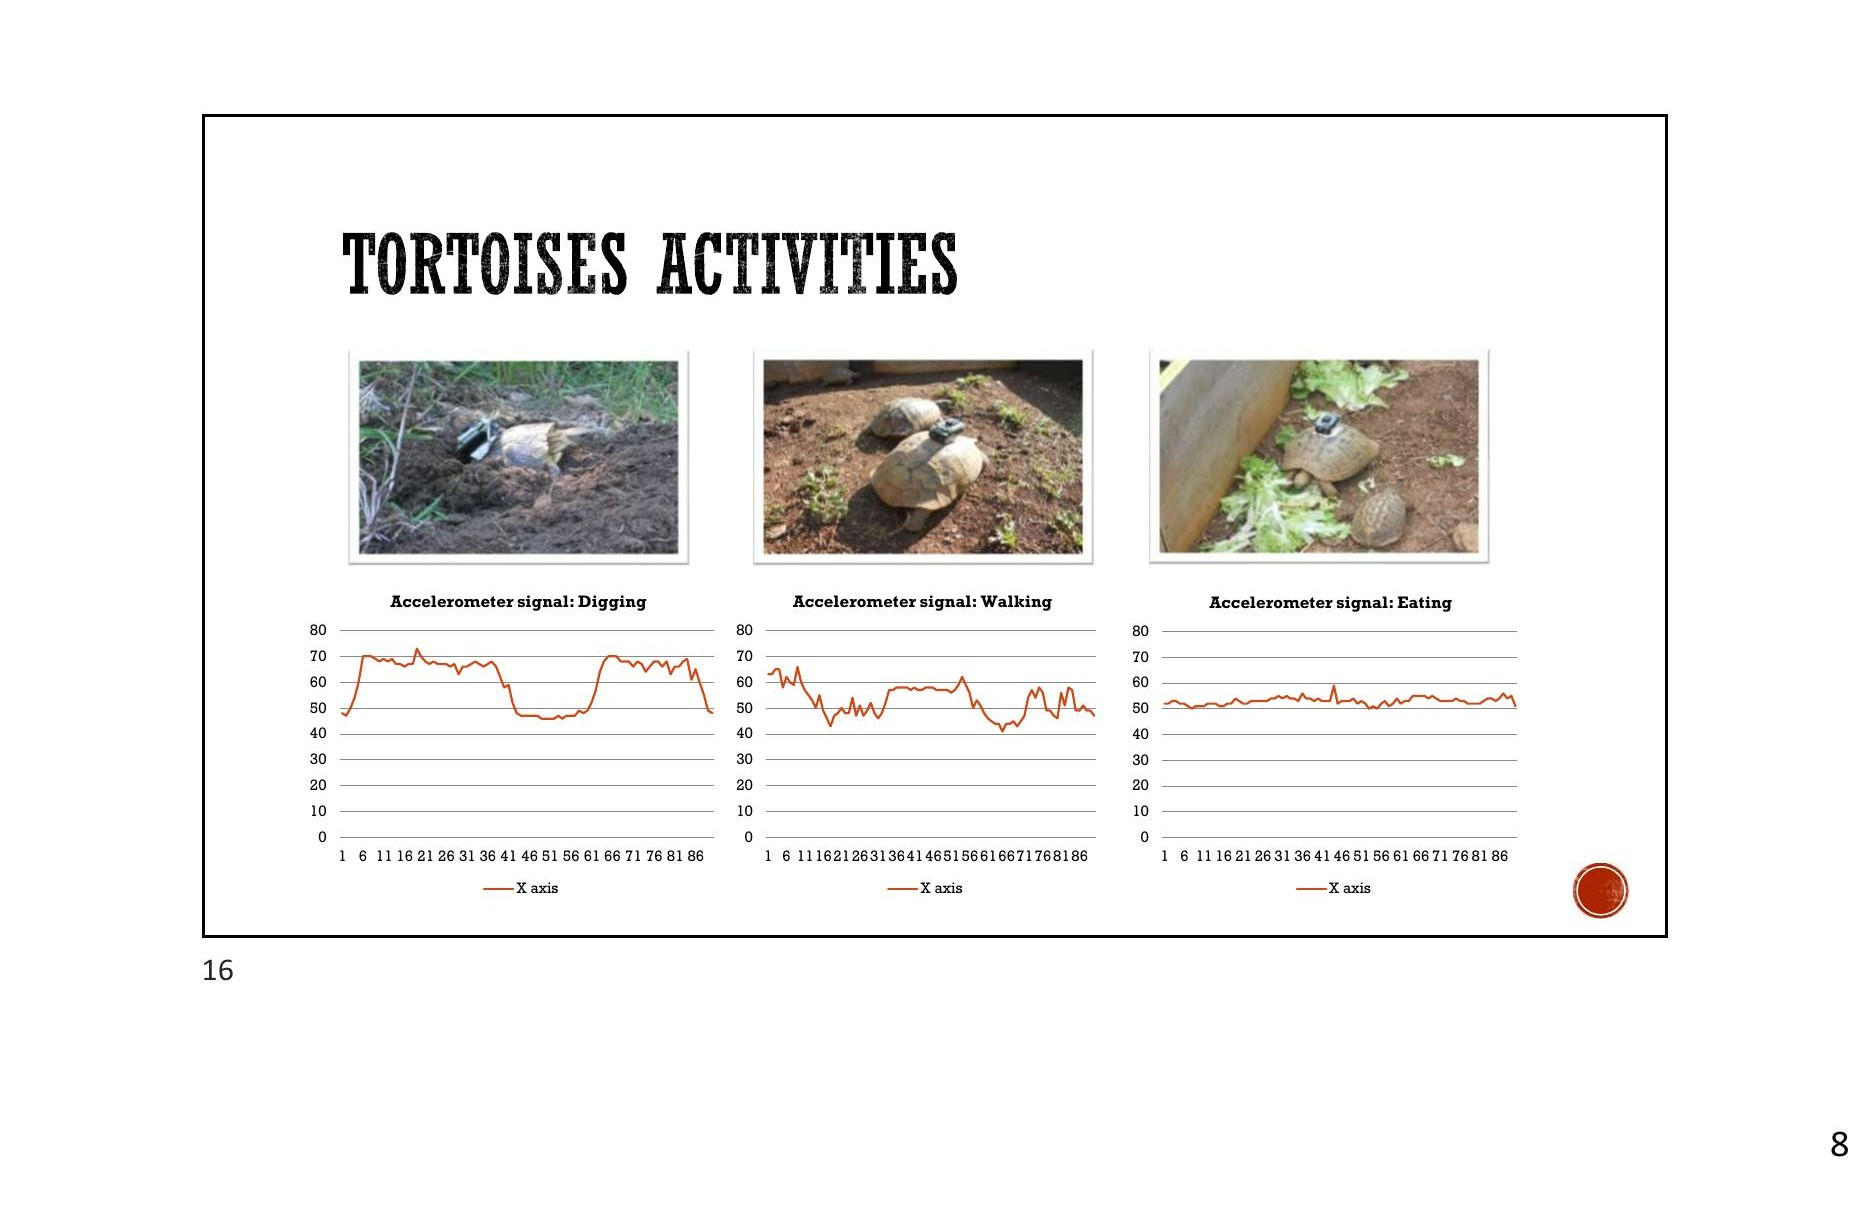
\includegraphics[keepaspectratio,alt={Segnali accelerometrici per scavo, camminata, alimentazione}]{images/lezione-19-caso-studio-tartarughe-img-05.jpg}}

\textbf{Risultati (Task asincrono 300 sec)}:
\pandocbounded{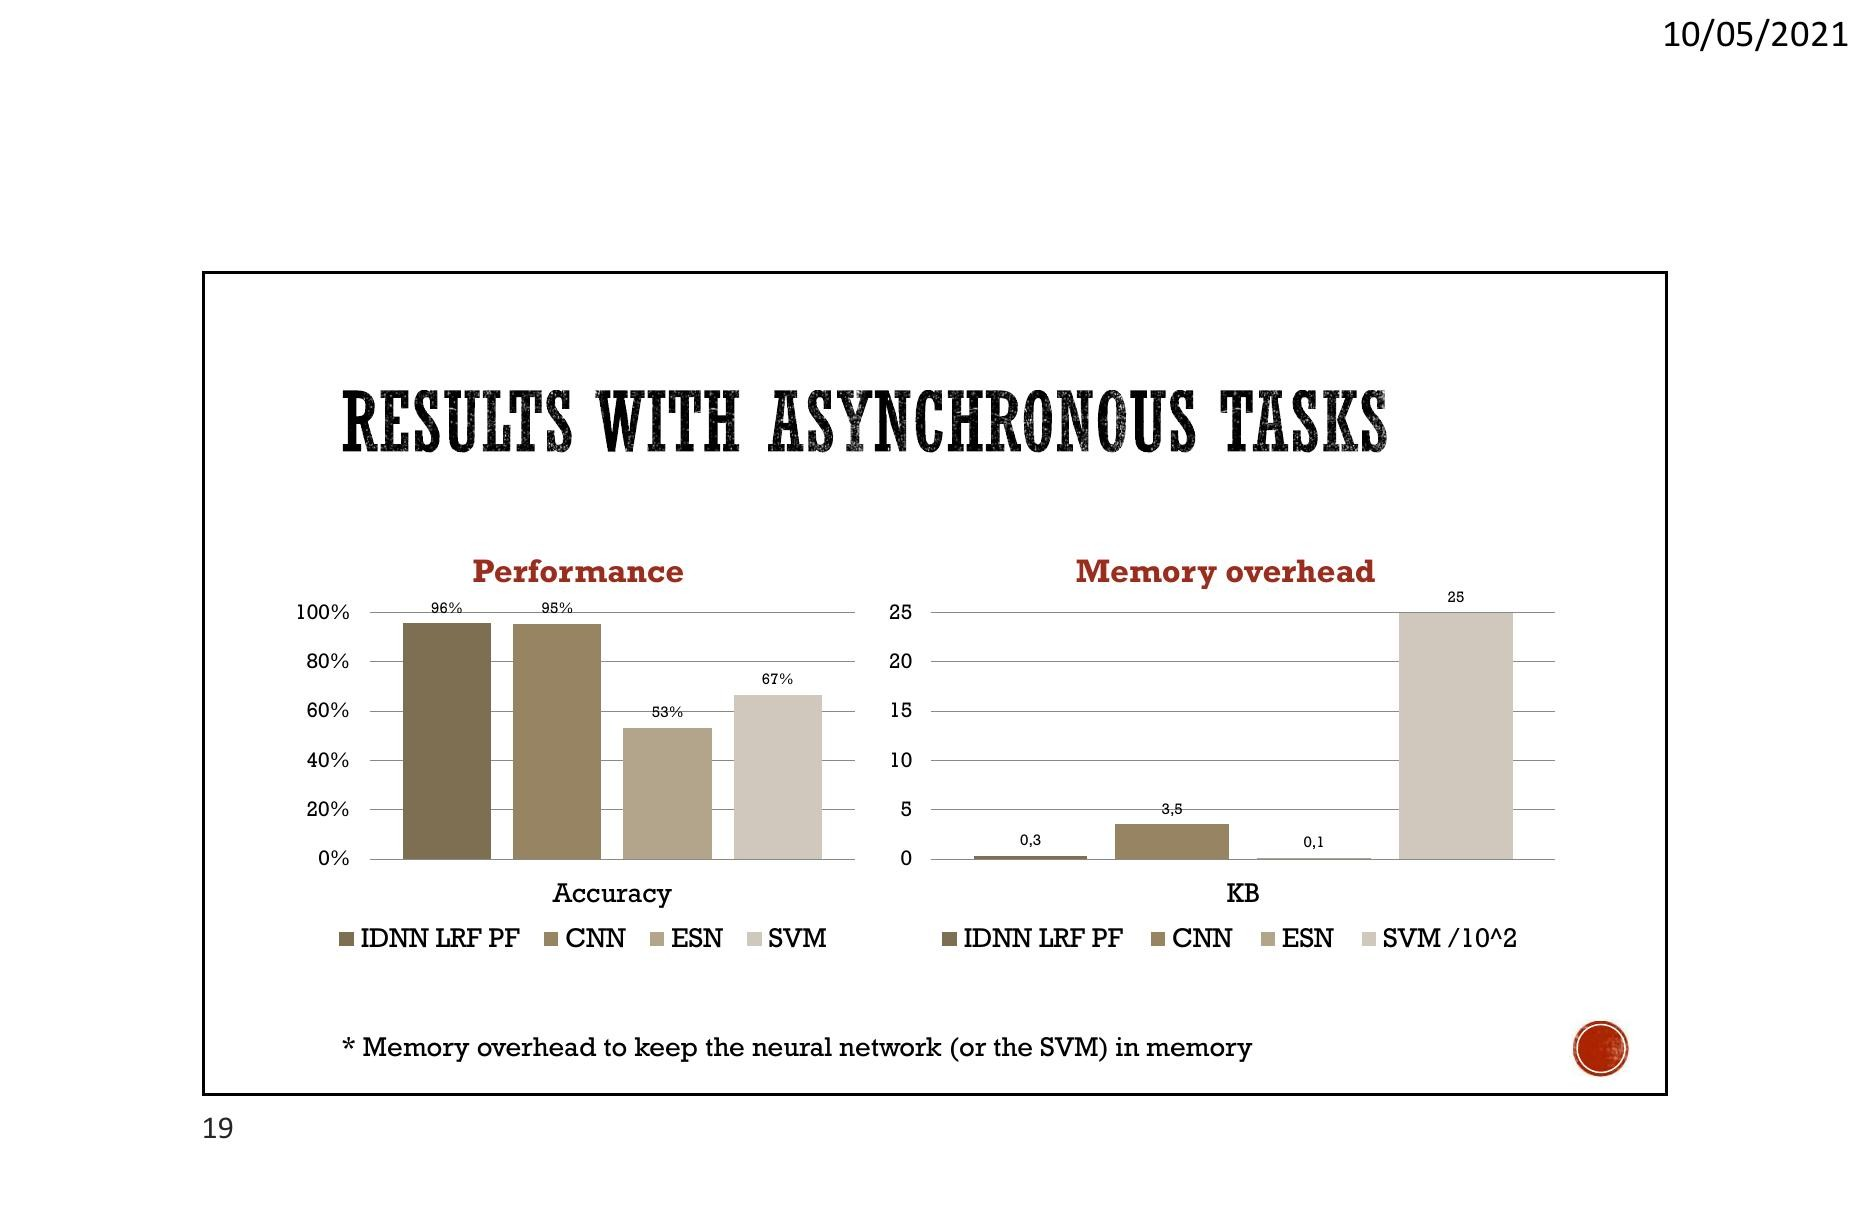
\includegraphics[keepaspectratio,alt={Risultati task asincrono}]{images/lezione-19-caso-studio-tartarughe-img-06.jpg}}
- La rete \textbf{IDNN} ottiene il 95\% di accuratezza richiedendo solo
\textbf{0,3 KB} di RAM, battendo le CNN che ne chiedono 3,5 KB. Su MCU
piccoli è essenziale. SVM richiede decine di KB per i vettori.

\textbf{Risultati (Task sincrono in streaming)}:
\pandocbounded{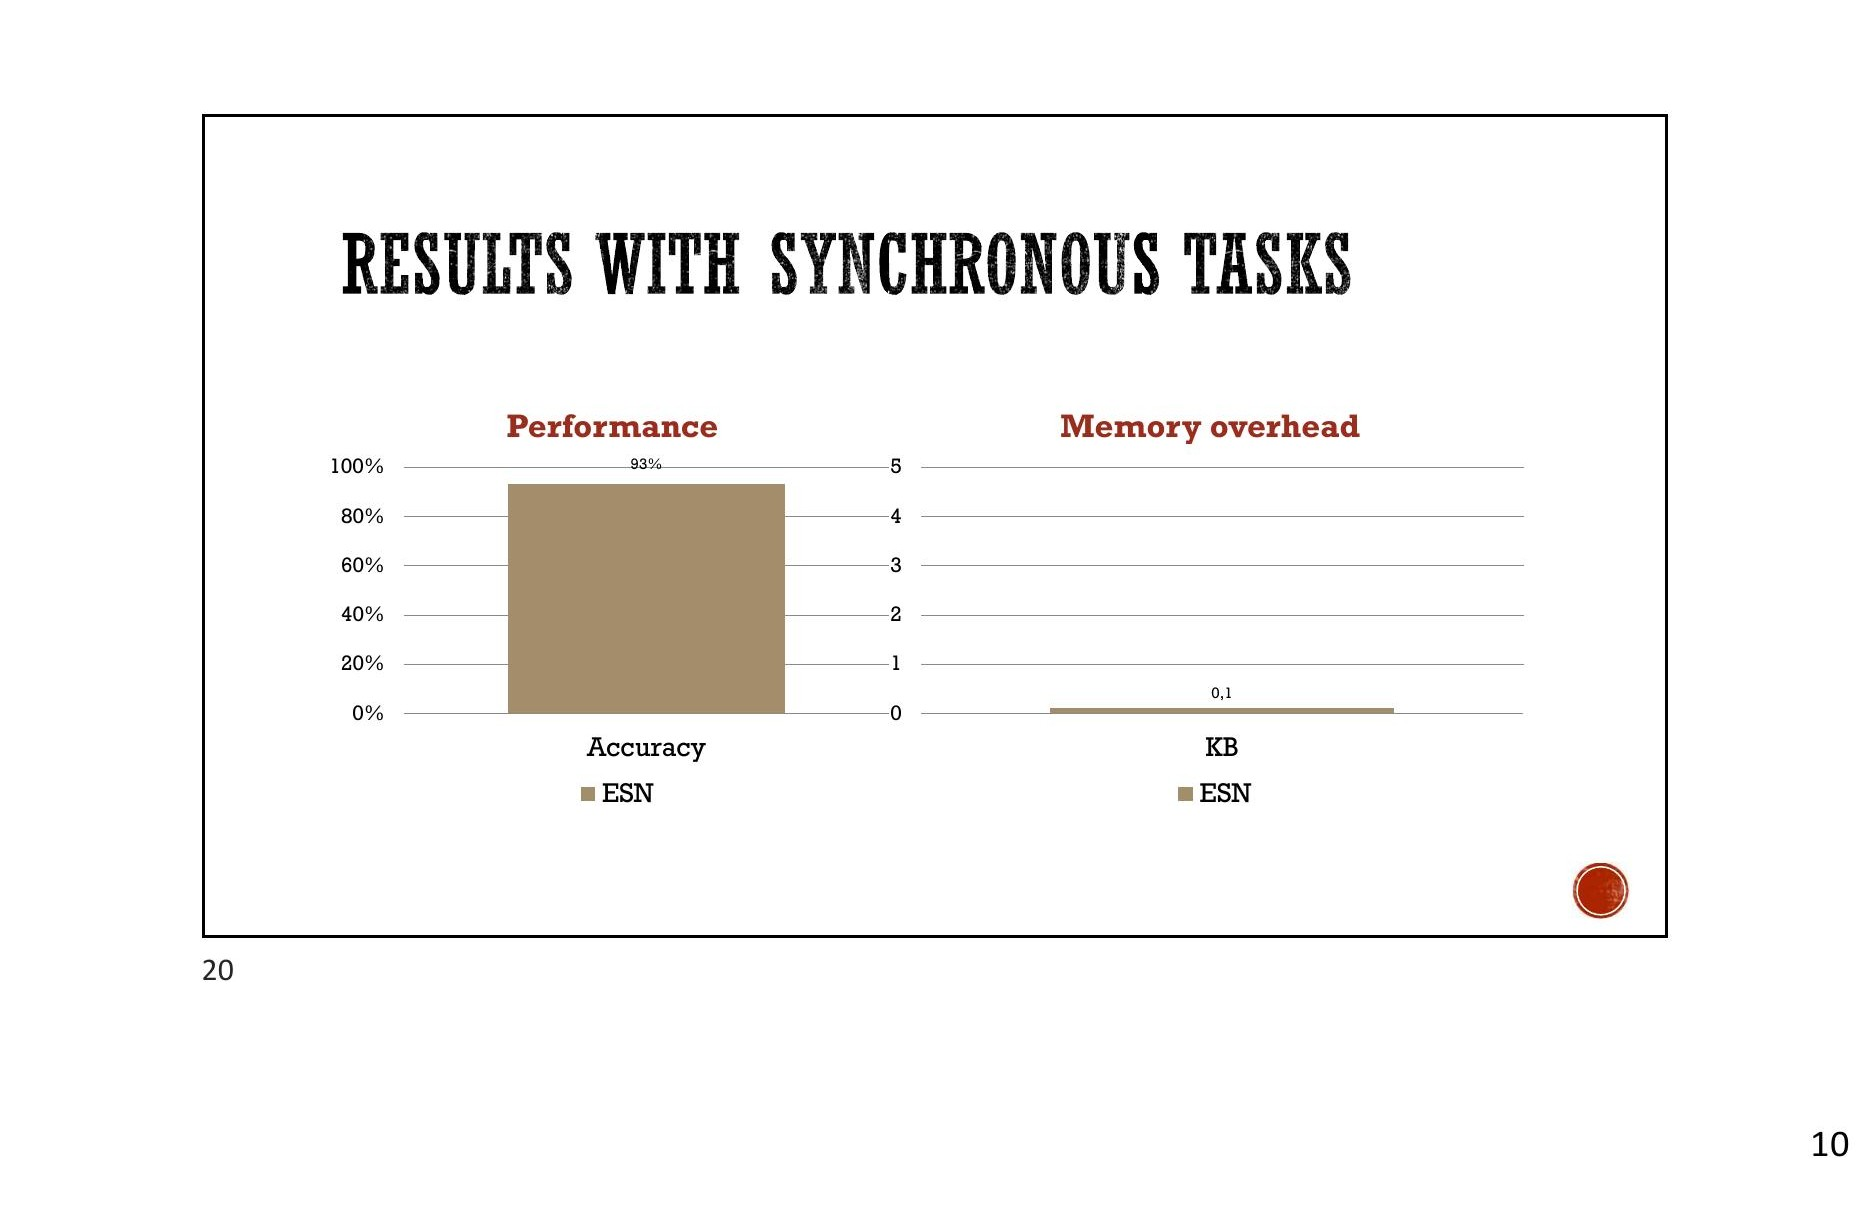
\includegraphics[keepaspectratio,alt={Risultati task sincrono}]{images/lezione-19-caso-studio-tartarughe-img-07.jpg}}
- Con \textbf{Echo State Network (ESN)}, accuratezza 93\% con appena
\textbf{0,1 KB di RAM}.

\begin{calloutnote}{Sintesi del risparmio}

Rispetto al cloud che richiede di trasmettere e/o memorizzare 13 MB,
Tortoise@ on-board conserva max 3 KB alla volta e usa il modulo radio
solo poche volte in 4 mesi.

\end{calloutnote}

\begin{center}\rule{0.5\linewidth}{0.5pt}\end{center}

\section{9. Embedded Programming e
Arduino}\label{embedded-programming-e-arduino}

Gli \textbf{sistemi embedded} sono progettati per svolgere una funzione
dedicata, tramite co-design hardware-software, che integra
microprocessori (microcontrollori) operanti a basso livello per fornire
il controllo del dispositivo ospite. A causa dei vincoli (spesso senza
un OS vero e proprio), si richiedono requisiti stringenti di
\textbf{Real-Time} (la correttezza temporale è essenziale quanto quella
logica) e di alta tolleranza ai fault.

\subsection{Cross-Compilazione e Modelli di
Esecuzione}\label{cross-compilazione-e-modelli-di-esecuzione}

\begin{figure}
\centering
\pandocbounded{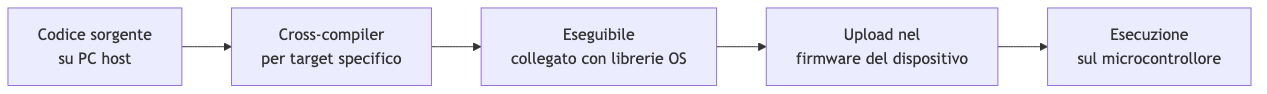
\includegraphics[keepaspectratio,alt={Pipeline di sviluppo per sistemi embedded, dal codice sorgente su PC host fino all'esecuzione sul microcontrollore}]{images/mermaid-01-fondamenti-iot-e-progettazione-01.png}}
\caption{Pipeline di sviluppo per sistemi embedded, dal codice sorgente
su PC host fino all'esecuzione sul microcontrollore}
\end{figure}

Poiché scarseggia RAM (es. Arduino Uno ha solo 2 KB), usare multipli
thread dotati di stack separati non è sostenibile. Due modelli
principali emergono:

\subsection{Il Modello Arduino}\label{il-modello-arduino}

Event loop sincrono a singolo thread. \texttt{loop()} viene iterato
indefinitamente.

\begin{figure}
\centering
\pandocbounded{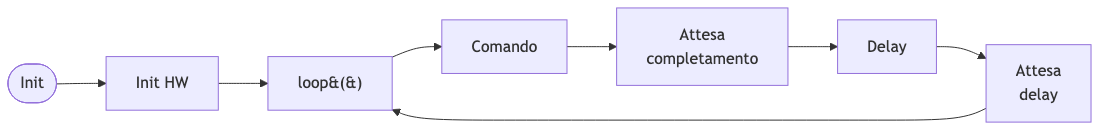
\includegraphics[keepaspectratio,alt={Modello di esecuzione di Arduino basato su singolo thread, esecuzione sequenziale e polling sincrono.}]{images/mermaid-01-fondamenti-iot-e-progettazione-02.png}}
\caption{Modello di esecuzione di Arduino basato su singolo thread,
esecuzione sequenziale e polling sincrono.}
\end{figure}

\subsection{Il Modello TinyOS}\label{il-modello-tinyos}

Progettato per efficienza e modularità asincrona senza thead overhead.
Sviluppato in tre entità: - \textbf{Comandi}: funzioni down-ward verso
l'hardware. - \textbf{Eventi}: up-call che astraggono interrupt
pre-emptando il flusso. - \textbf{Task}: coda sequenziale non-preemptive
per il lavoro deferito dagli event handlers.

\begin{figure}
\centering
\pandocbounded{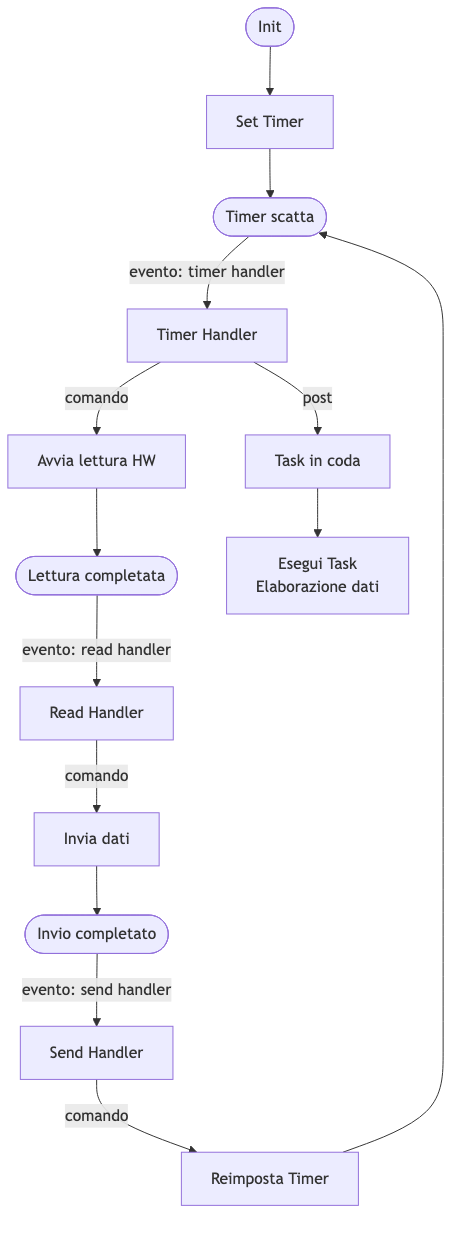
\includegraphics[keepaspectratio,alt={Flusso di esecuzione basato su eventi in TinyOS, in cui gli eventi gestiscono immediatamente l'hardware e delegano l'elaborazione ai task asincroni.}]{images/mermaid-01-fondamenti-iot-e-progettazione-03.png}}
\caption{Flusso di esecuzione basato su eventi in TinyOS, in cui gli
eventi gestiscono immediatamente l'hardware e delegano l'elaborazione ai
task asincroni.}
\end{figure}

\begin{figure}
\centering
\pandocbounded{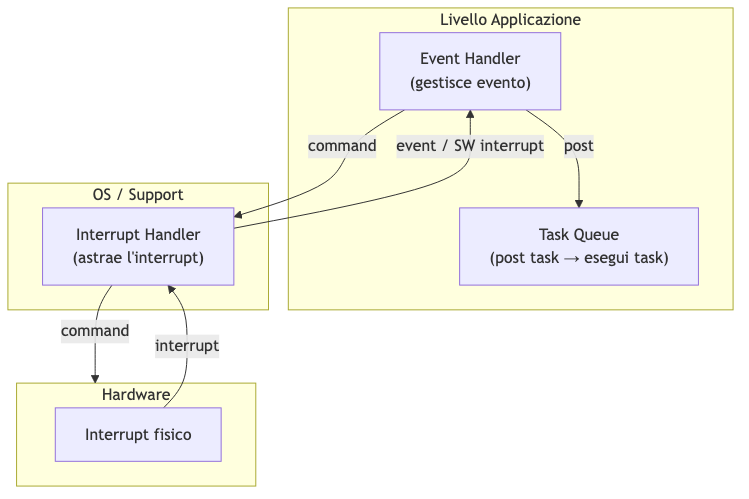
\includegraphics[keepaspectratio,alt={Modello a tre livelli per la gestione degli eventi nei sistemi embedded, in cui l'hardware genera interrupt, il sistema operativo li astrae in eventi e l'applicazione li gestisce tramite event handler e task.}]{images/mermaid-01-fondamenti-iot-e-progettazione-04.png}}
\caption{Modello a tre livelli per la gestione degli eventi nei sistemi
embedded, in cui l'hardware genera interrupt, il sistema operativo li
astrae in eventi e l'applicazione li gestisce tramite event handler e
task.}
\end{figure}

\subsection{Arduino e Interrupt
Esterni}\label{arduino-e-interrupt-esterni}

La piattaforma Arduino Uno basa tutto sul ATmega328.

\begin{figure}
\centering
\pandocbounded{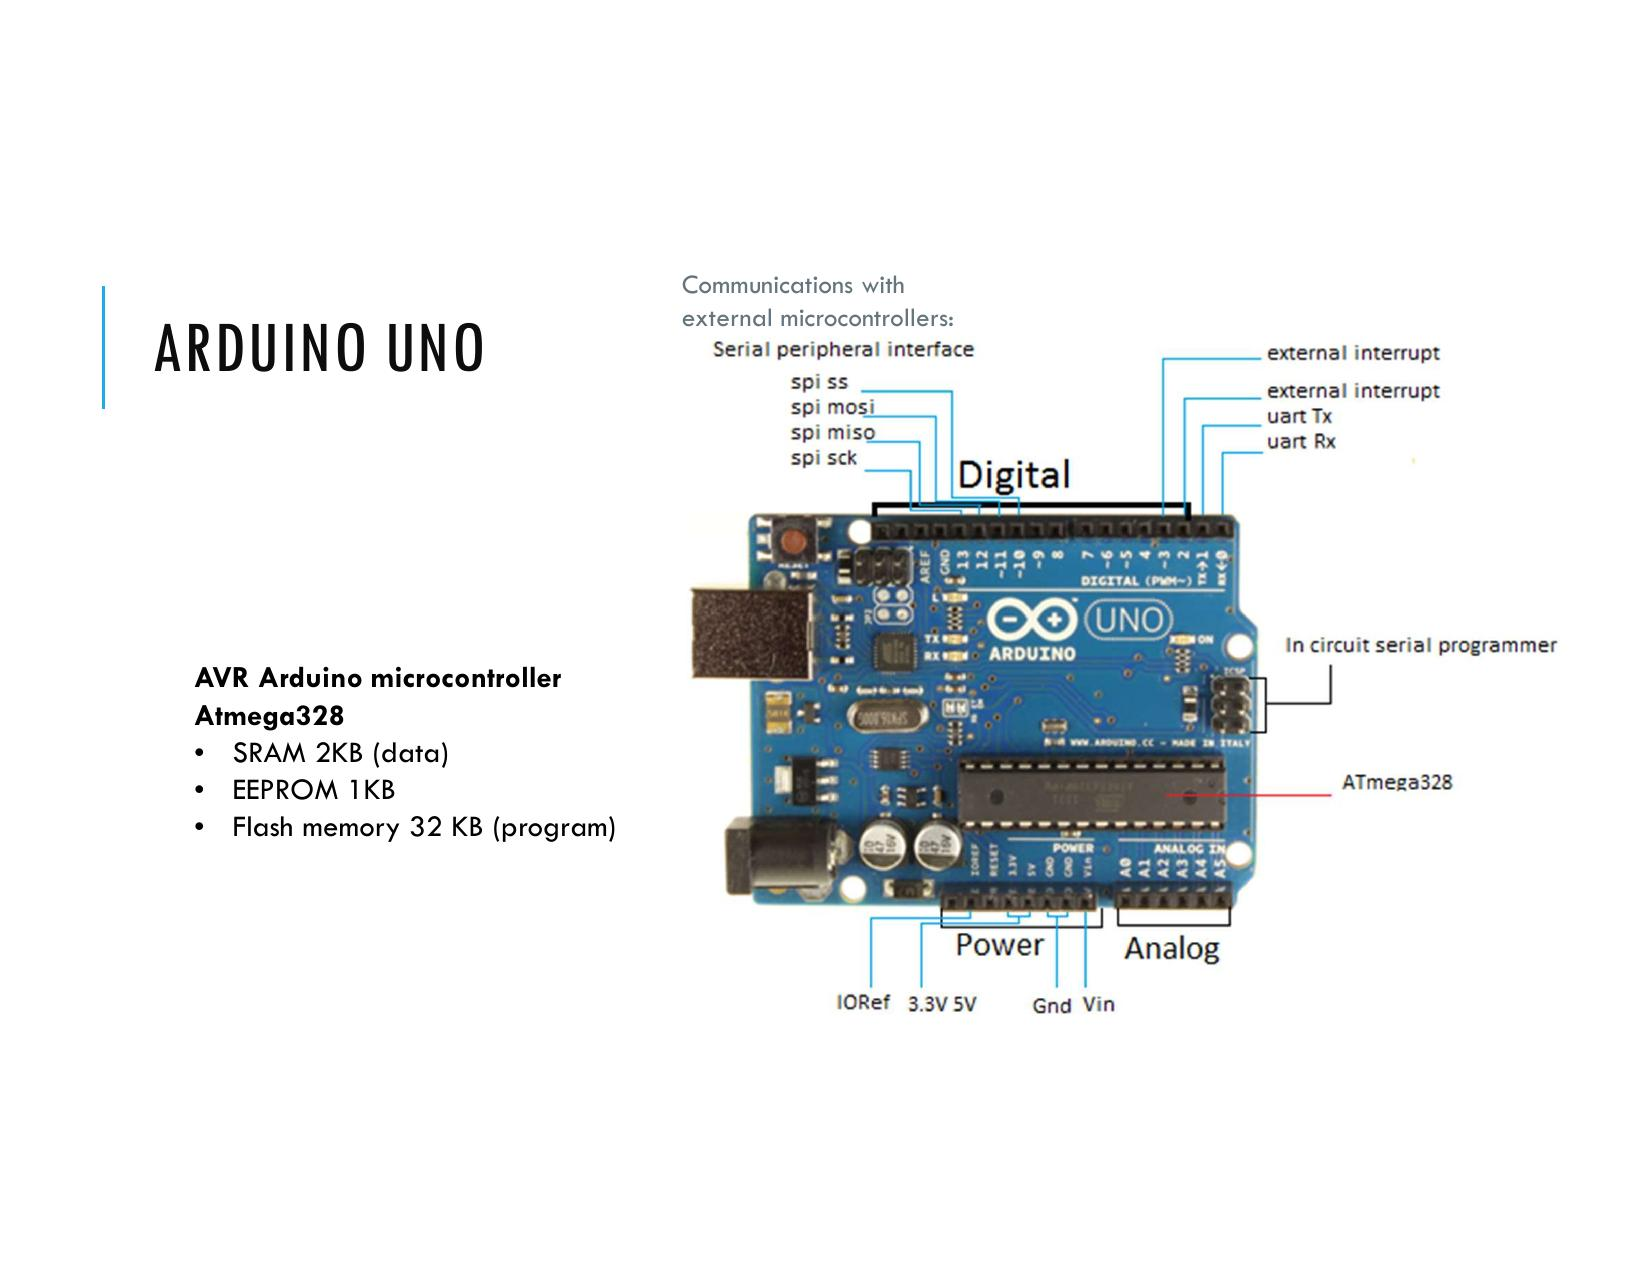
\includegraphics[keepaspectratio,alt={Scheda Arduino Uno con pinout annotato}]{images/lezione-23-embedded-programming-e-arduino-img-01.jpg}}
\caption{Scheda Arduino Uno con pinout annotato}
\end{figure}

Oltre al bloccante \texttt{delay()}, offre gestione asincrona tramite
gli \textbf{interrupt esterni} (\texttt{attachInterrupt()}) sui pin
digitali 2 e 3. Regole vitali per i gestori di interrupt
(\emph{handler}): - Devono essere rapidissimi, delegando tutto il lavoro
extra. - Dentro l'handler \texttt{delay()} o le funzioni basate su
\texttt{millis()} non funzionano. - Le variabili modificate nell'handler
e lette nel loop devono essere marcate come \texttt{volatile} in C,
imponendo letture forzate in RAM.

\begin{figure}
\centering
\pandocbounded{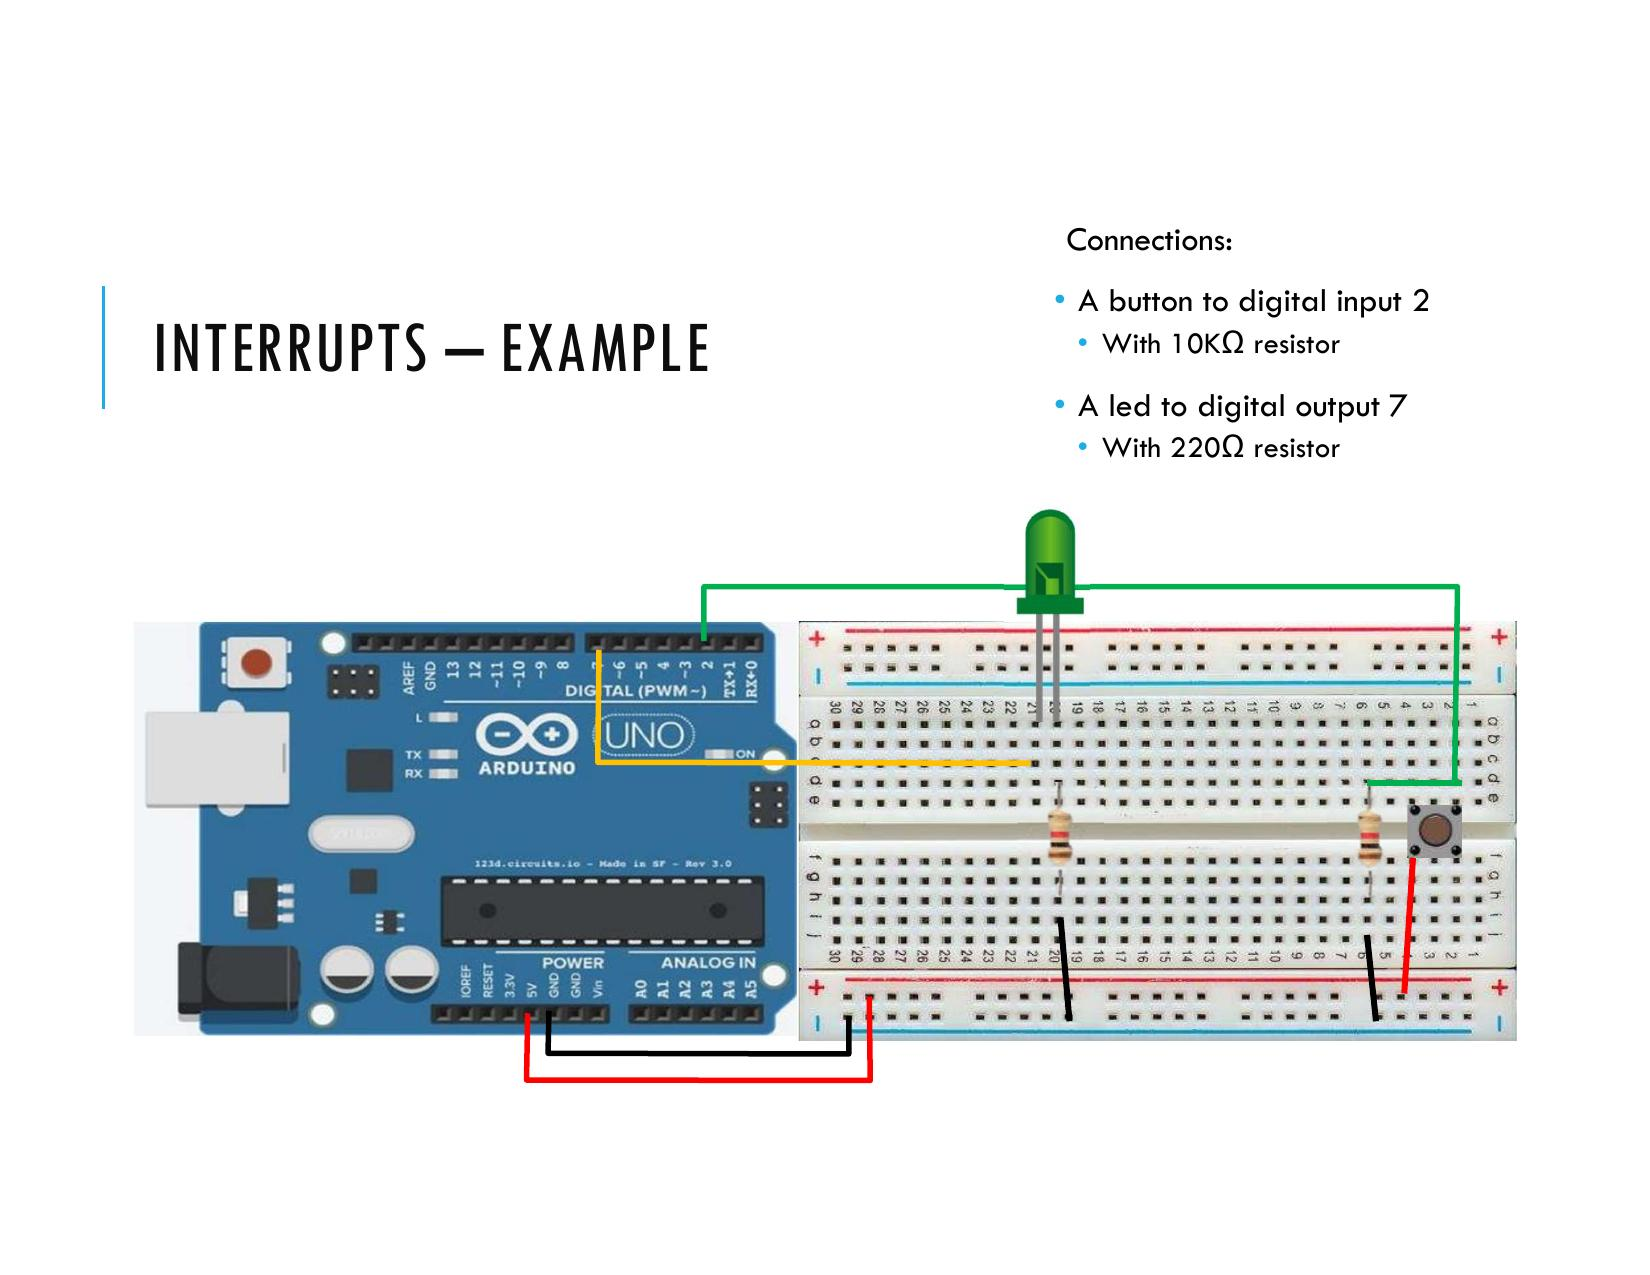
\includegraphics[keepaspectratio,alt={Schema circuito Arduino con interrupt}]{images/lezione-23-embedded-programming-e-arduino-img-02.jpg}}
\caption{Schema circuito Arduino con interrupt}
\end{figure}

\subsection{Sleep Mode in Arduino}\label{sleep-mode-in-arduino}

L'ATmega328P supporta vari Sleep mode gestibili tramite
\emph{LowPower.h}. Il più utile e profondo per azzerare il DC in
inattività è \textbf{Power-Down}, che spegne il clock principale
consentendo risvegli unicamente tramite interrupt esterni.

\begin{center}\rule{0.5\linewidth}{0.5pt}\end{center}

\section{10. Domande d'esame frequenti}\label{domande-desame-frequenti}

\begin{itemize}
\tightlist
\item
  Cos'è un Cyber-Physical System e in cosa si distingue da un sistema
  puramente informatico o fisico?
\item
  Descrivere le quattro generazioni di Internet e le caratteristiche che
  differenziano l'IoT.
\item
  Quali funzionalità offre una piattaforma IoT e perché è necessario uno
  strato software intermedio?
\item
  Cosa si intende per vendor lock-in e vertical silos?
\item
  Quali sono le tre macro-categorie di scenari d'uso del 5G?
\item
  Descrivere le configurazioni di integrazione Tipo A, B, C e D: quando
  è necessario un gateway applicativo?
\item
  Quali sono i requisiti di sicurezza (ITU-T Y.2066) e qual è il ruolo
  del gateway?
\item
  Quali sono le differenze tra Edge, Fog e Cloud Computing nell'IoT?
\item
  Come funziona il Federated Learning e quali sono i principali attacchi
  a cui è soggetto?
\item
  Perché i database NoSQL sono preferiti ai DB relazionali nei contesti
  IoT?
\item
  Quali sono le tre interpretazioni della Legge di Moore e come si
  applicano all'IoT?
\item
  Perché tenere la radio in modalità ``listen'' è quasi costoso quanto
  ricevere dati?
\item
  Come si calcola il duty cycle di un componente e qual è il trade-off
  tra edge processing e offloading in cloud?
\item
  Qual è la differenza tra biotelemetria e bio-logging?
\item
  Come funziona la macchina a stati di Tortoise@ per ottimizzare
  l'efficienza energetica e confronta IDNN, CNN, ESN e SVM.
\item
  Quali sono le principali differenze tra un sistema embedded e un PC
  general purpose e in cosa consiste il co-design?
\item
  Confrontare il modello Arduino con il modello TinyOS (eventi, comandi
  e task).
\item
  Quali regole vanno rispettate nello scrivere un Interrupt Handler (es.
  \texttt{volatile}, blocchi)?
\item
  Descrivere le modalità di sleep dell'ATmega328P.
\end{itemize}

\newpage

\chapter{02 - Protocolli Applicativi (MQTT e
CoAP)}\label{protocolli-applicativi-mqtt-e-coap}

Questa lezione analizza l'evoluzione delle architetture di rete e degli
stack di protocolli pensati per l'Internet of Things, culminando con
un'analisi strutturale del protocollo MQTT e del protocollo CoAP.
Vengono esplorati i paradigmi di comunicazione, le logiche di
connessione, la strutturazione dei topic e i meccanismi di affidabilità.

\section{I Requisiti dell'IoT e la Conventional Internet Protocol
Suite}\label{i-requisiti-delliot-e-la-conventional-internet-protocol-suite}

Perché un oggetto diventi a tutti gli effetti un dispositivo IoT deve
essere connesso a Internet. Tradizionalmente, i sistemi si interfacciano
alla rete globale tramite la \textbf{Internet protocol suite}
convenzionale, strutturata sul binomio TCP/IP affiancato da un livello
applicativo come HTTP. Questa suite si articola su tre livelli: il
\textbf{livello di rete} (\textbf{IP} per indirizzamento e routing
best-effort); il \textbf{livello di trasporto} (\textbf{TCP} per
garanzie di consegna o \textbf{UDP} per minor overhead); il
\textbf{livello applicativo} (\textbf{HTTP} con architettura
client/server).

Questo stack è stato pensato per dispositivi \emph{resource-rich}. Per i
nodi IoT risulta troppo pesante: operano su reti instabili
(\emph{lossy}), con hardware a bassissimo consumo energetico (\emph{low
power}) e risorse estremamente limitate (\emph{constrained}). Questi
vincoli impongono una ridefinizione completa dei requisiti:

{\def\LTcaptype{none} % do not increment counter
\begin{longtable}[]{@{}
  >{\raggedright\arraybackslash}p{(\linewidth - 2\tabcolsep) * \real{0.5000}}
  >{\raggedright\arraybackslash}p{(\linewidth - 2\tabcolsep) * \real{0.5000}}@{}}
\toprule\noalign{}
\begin{minipage}[b]{\linewidth}\raggedright
Requisiti di Rete
\end{minipage} & \begin{minipage}[b]{\linewidth}\raggedright
Impatto sul Networking
\end{minipage} \\
\midrule\noalign{}
\endhead
\bottomrule\noalign{}
\endlastfoot
\textbf{Scalabilità / Ridondanza} & Necessità di reti multi-hop e
architetture mesh. \\
\textbf{Sicurezza} & Deve essere configurabile in base alle capacità dei
singoli dispositivi. \\
\textbf{Indirizzamento} & Richiede uno spazio di indirizzamento
scalabile e protocolli a basso overhead. \\
\textbf{Requisiti del Dispositivo} & \textbf{Impatto sul Livello
Applicativo} \\
\textbf{Basso consumo / A batteria} & Progettazione di applicazioni con
basso duty-cycle. \\
\textbf{Capacità limitata (memoria/CPU)} & Necessità di protocolli con
footprint minimo e bassa complessità. \\
\textbf{Basso costo} & Aumenta la richiesta di affidabilità,
introducendo ulteriori vincoli fisici. \\
\end{longtable}
}

\begin{center}\rule{0.5\linewidth}{0.5pt}\end{center}

\section{Introduzione al Protocollo
MQTT}\label{introduzione-al-protocollo-mqtt}

\begin{calloutdefinition}{MQTT}

\textbf{MQTT} (\emph{Message Queuing Telemetry Transport}) è un
protocollo di messaggistica leggero di tipo publish/subscribe,
progettato per ambienti con risorse limitate e connettività instabile.
Standardizzato da OASIS (versione di riferimento 3.1.1).

\end{calloutdefinition}

Ideato nel 1999, la sua leggerezza si manifesta in tre modi: code
footprint ridotto, basso consumo di banda e overhead di pacchetto
minimo. MQTT si appoggia su TCP/IP operando sulla \textbf{porta 1883} in
chiaro e sulla \textbf{porta 8883} in \textbf{SSL/TLS} (che introduce un
overhead computazionale significativo per le MCU).

Il protocollo concentra la complessità sul lato server (il broker),
mantenendo l'implementazione client semplice. È \emph{data agnostic}
(non si cura del payload) e implementa meccanismi di garanzia della
consegna (QoS).

\begin{center}\rule{0.5\linewidth}{0.5pt}\end{center}

\section{Il Paradigma Publish /
Subscribe}\label{il-paradigma-publish-subscribe}

\begin{callouttip}{Pub/Sub e i tre disaccoppiamenti}

Il paradigma introduce tre forme di \emph{decoupling} ideali per l'IoT:
- \textbf{Space decoupling}: publisher e subscriber non si conoscono
(non condividono IP/porta). - \textbf{Time decoupling}: non devono
essere operativi contemporaneamente. - \textbf{Synchronization
decoupling}: le operazioni sui client non sono bloccanti durante publish
o receive.

\end{callouttip}

Il paradigma pub/sub è \emph{loosely coupled}. I \textbf{publisher} e i
\textbf{subscriber} agiscono come client. Il \textbf{broker} riceve
tutti i messaggi, li filtra e li distribuisce. Le operazioni cardine
sono quattro: \emph{Publish}, \emph{Subscribe}, \emph{Notify} e
\emph{Unsubscribe}.

La scalabilità è superiore rispetto all'architettura client/server. Le
modalità di filtraggio sono tre: \textbf{topic-based} (MQTT),
\textbf{content-based} (il broker ispeziona il payload, ma impedisce la
cifratura), e \textbf{type-based} (filtraggio semantico, richiede forte
integrazione col linguaggio). Publisher e subscriber devono accordarsi
\emph{a priori} sui topic, e il publisher non può assumere che ci sia
qualcuno in ascolto.

\begin{center}\rule{0.5\linewidth}{0.5pt}\end{center}

\section{Il Modello MQTT: Connessione e Flusso
Operativo}\label{il-modello-mqtt-connessione-e-flusso-operativo}

\begin{figure}
\centering
\pandocbounded{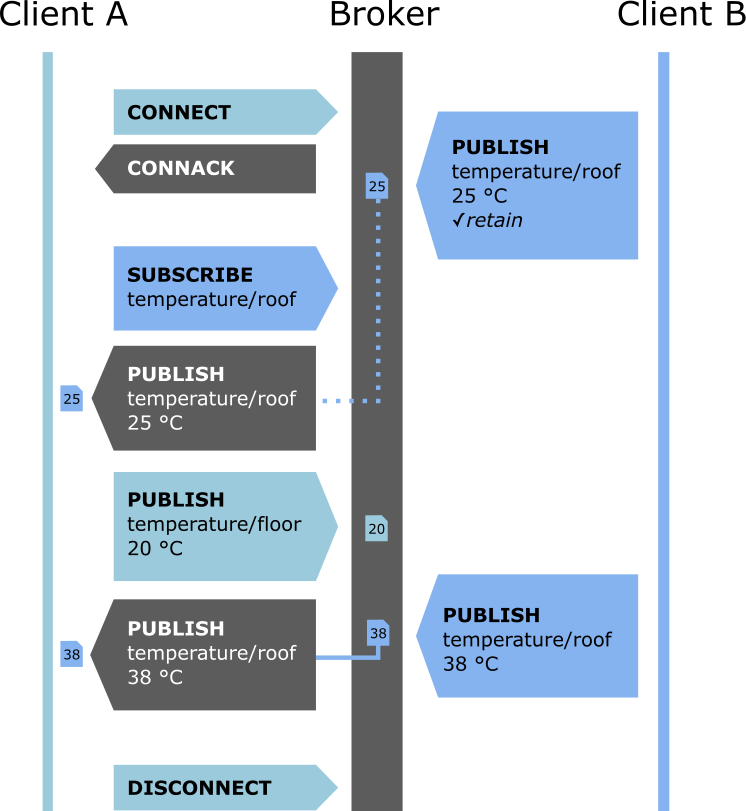
\includegraphics[keepaspectratio]{images/MQTT_protocol_example_without_QoS.png}}
\caption{Fonte: Wikimedia Commons --- Il flusso completo: Client A si
connette, Client B si sottoscrive, Client A pubblica.}
\end{figure}

\begin{figure}
\centering
\pandocbounded{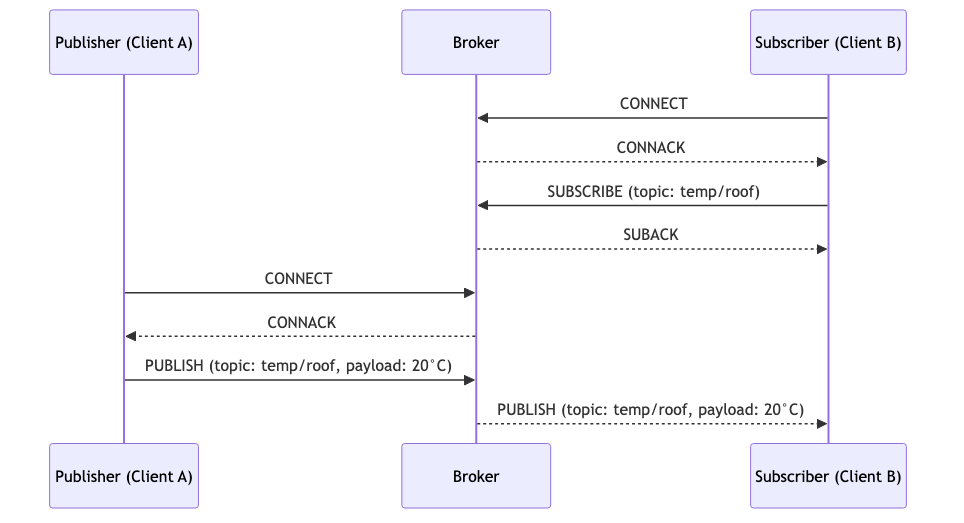
\includegraphics[keepaspectratio,alt={Questo schema illustra il flusso base di interazione tra publisher, broker e subscriber in MQTT, mostrando la connessione, sottoscrizione e pubblicazione dei dati.}]{images/mermaid-02-protocolli-applicativi-01.png}}
\caption{Questo schema illustra il flusso base di interazione tra
publisher, broker e subscriber in MQTT, mostrando la connessione,
sottoscrizione e pubblicazione dei dati.}
\end{figure}

L'infrastruttura opera ai livelli 5-6 (ISO/OSI), sopra TCP. I
dispositivi devono conoscere hostname e porta del broker in anticipo.

\subsection{L'Instaurazione della
Connessione}\label{linstaurazione-della-connessione}

Il client invia il pacchetto \textbf{CONNECT}: - \textbf{Client ID}
(obbligatorio): univoco. Se vuoto, richiede \emph{Clean Session} a
\texttt{true}. - \textbf{Clean Session} (opzionale): \texttt{false}
richiede una \emph{persistent session} (salva stato, iscrizioni e QoS ≥
1). - \textbf{Username/Password} (opzionali): per autenticazione (in
chiaro senza TLS). - \textbf{Will flags} (opzionali): testamento per
disconnessioni anomale. - \textbf{KeepAlive} (opzionale): timeout (in
secondi) entro cui inviare almeno un pacchetto (ping).

Il broker risponde con \textbf{CONNACK} (Connect Acknowledgement),
contenente i flag \emph{Connection Accepted/Refused} e \emph{Session
Present}.

\subsection{Sottoscrizione e
Ricezione}\label{sottoscrizione-e-ricezione}

Un client invia \textbf{SUBSCRIBE} contenente un \texttt{packetId} e
l'elenco dei topic con il QoS richiesto. Il broker risponde con
\textbf{SUBACK} (ritorna \texttt{128} per fallimento, o \texttt{0},
\texttt{1}, \texttt{2} per successo col \emph{maximum QoS granted}). Per
revocare si usa \textbf{UNSUBSCRIBE} (risposta \textbf{UNSUBACK}).

\subsection{Gestione e Best Practices dei
Topic}\label{gestione-e-best-practices-dei-topic}

Gerarchia separata dal carattere \texttt{/}. I subscriber possono usare
le \textbf{wildcard}: - \textbf{\texttt{+}}: sostituisce un singolo
livello (es. \texttt{home/+/presence}). - \textbf{\texttt{\#}}:
sostituisce tutti i livelli successivi (es. \texttt{home/\#}). I topic
che iniziano con \texttt{\$} sono riservati al broker per statistiche
(es. \texttt{\$SYS/broker/uptime}).

\begin{calloutwarning}{Best practices per i topic}

- Non iniziare il topic con \texttt{/} (es. \texttt{/home}). - Non usare
spazi; mantenere le stringhe corte; usare ASCII/UTF-8. - Includere il
\texttt{clientId} (es. \texttt{sensor1/temperature}) per limitare i
permessi. - Usare topic specifici anziché aggregati. - Evitare l'abuso
del wildcard \texttt{\#}.

\end{calloutwarning}

\subsection{Pubblicazione}\label{pubblicazione}

Messaggio \textbf{PUBLISH}: - \textbf{topicName}: stringa del topic di
destinazione. - \textbf{payload}: dati (binari, testo, JSON). -
\textbf{packetId}: 16 bit, usato per QoS \textgreater{} 0. -
\textbf{retainFlag}: se attivo, il broker conserva l'ultimo messaggio
per i nuovi subscriber. - \textbf{dupFlag}: duplicato per
ritrasmissioni. - \textbf{qos}: livello di Quality of Service.

\begin{center}\rule{0.5\linewidth}{0.5pt}\end{center}

\section{I Meccanismi della Quality of Service
(QoS)}\label{i-meccanismi-della-quality-of-service-qos}

Il QoS regola la garanzia di consegna. È importante notare che il QoS
tra publisher e broker è indipendente da quello tra broker e subscriber.
I messaggi sono tracciati da un \texttt{packetId} a 16 bit.

\begin{calloutnote}{I tre livelli QoS a confronto}

{\def\LTcaptype{none} % do not increment counter
\begin{longtable}[]{@{}lllll@{}}
\toprule\noalign{}
Livello & Nome & Garanzia & Meccanismo & Duplicati \\
\midrule\noalign{}
\endhead
\bottomrule\noalign{}
\endlastfoot
\textbf{QoS 0} & At most once & Nessuna & Nessun ACK, no mem. & No \\
\textbf{QoS 1} & At least once & Almeno una & PUBACK & Possibili \\
\textbf{QoS 2} & Exactly once & Esattamente una & Handshake a 4 fasi &
No \\
\end{longtable}
}

\end{calloutnote}

\begin{itemize}
\tightlist
\item
  \textbf{QoS 0}: Modalità \emph{best effort}. Ottima per dati che
  invecchiano rapidamente.
\item
  \textbf{QoS 1}: Il broker memorizza il messaggio e risponde con
  \textbf{PUBACK}. Se l'ACK non arriva, si ritrasmette con
  \texttt{dupFlag} attivo (possibili duplicati).
\item
  \textbf{QoS 2}: Elimina duplicati e garantisce singola consegna.
  Comporta un handshake a quattro fasi: \textbf{PUBLISH} →
  \textbf{PUBREC} → \textbf{PUBREL} → \textbf{PUBCOMP}.
\end{itemize}

\begin{figure}
\centering
\pandocbounded{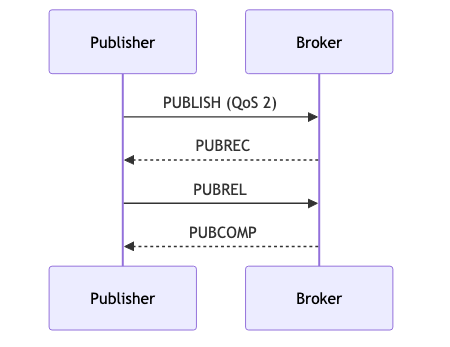
\includegraphics[keepaspectratio,alt={Flusso di messaggi nel QoS 2 per garantire una singola consegna esatta tra client e broker, evitando perdita di dati e duplicati.}]{images/mermaid-02-protocolli-applicativi-02.png}}
\caption{Flusso di messaggi nel QoS 2 per garantire una singola consegna
esatta tra client e broker, evitando perdita di dati e duplicati.}
\end{figure}

\begin{center}\rule{0.5\linewidth}{0.5pt}\end{center}

\section{Meccanismi di Affidabilità
Avanzati}\label{meccanismi-di-affidabilituxe0-avanzati}

\subsection{Sessioni Persistenti}\label{sessioni-persistenti}

Se \emph{Clean Session} è \texttt{false}, il broker salva per il
\texttt{clientId} le sottoscrizioni e i messaggi non consegnati (QoS
1/2). Anche il \textbf{client} deve salvare i messaggi non-acked. Non
vanno usate se si pubblica solo a QoS 0 o se perdere messaggi vecchi è
tollerabile.

\subsection{\texorpdfstring{Messaggi Trattenuti (\emph{Retained
Messages})}{Messaggi Trattenuti (Retained Messages)}}\label{messaggi-trattenuti-retained-messages}

Messaggi inviati con \textbf{\texttt{retainFlag\ =\ true}}. Il broker ne
mantiene uno per topic e lo invia istantaneamente a ogni nuovo iscritto
(utile per trasmettere lo stato attuale senza aspettare nuovi
aggiornamenti, es. dispositivo ``ON''). Indipendenti dalle sessioni
persistenti.

\subsection{Last Will \& Testament
(Testamento)}\label{last-will-testament-testamento}

Configurato durante la connessione (CONNECT) con i parametri
\texttt{lastWillTopic}, \texttt{lastWillQoS}, \texttt{lastWillMessage} e
\texttt{lastWillRetain}. Se il client si disconnette
\emph{anormalmente}, il broker pubblica il messaggio. Avviene per 4
cause: errore di I/O, PINGREQ mancato (keep alive), chiusura TCP brusca,
errore protocollo lato broker. (Se la disconnessione è tramite
DISCONNECT, viene scartato).

\subsection{Keep Alive}\label{keep-alive}

Mitiga il problema di TCP di non accorgersi dei peer offline. Il client
invia \textbf{PINGREQ} entro l'intervallo specificato in CONNECT, e il
broker risponde con \textbf{PINGRESP}.

\begin{center}\rule{0.5\linewidth}{0.5pt}\end{center}

\section{Struttura dei Pacchetti
MQTT}\label{struttura-dei-pacchetti-mqtt}

Ogni \textbf{MQTT Control Packet} comprende: 1. \textbf{Fixed Header}
(min 2 byte): - \textbf{Byte 1}: Tipo pacchetto (4 bit) + Flag (4 bit).
Es. nel PUBLISH i flag indicano DUP, QoS e Retain. Negli altri spesso è
\texttt{0,0,0,0} (eccetto PUBREL/SUBSCRIBE/UNSUBSCRIBE che usano
\texttt{0,0,1,0}). - \textbf{Byte 2+}: \emph{Remaining Length}
(lunghezza variabile). 2. \textbf{Variable Header}: Presente solo in
alcuni pacchetti (es. \texttt{packet\ identifier} di 2 byte per QoS
\textgreater{} 0). 3. \textbf{Payload}: Es. il
\texttt{client\ identifier} in CONNECT. È assente nei pacchetti di
controllo (PINGREQ, DISCONNECT, ACK QoS).

I tipi principali: CONNECT(1), CONNACK(2), PUBLISH(3),
PUBACK-PUBREC-PUBREL-PUBCOMP(4-7), SUBSCRIBE(8), SUBACK(9), ecc.

\begin{center}\rule{0.5\linewidth}{0.5pt}\end{center}

\section{Implementazione Pratica: MQTT su
Arduino}\label{implementazione-pratica-mqtt-su-arduino}

La libreria \textbf{PubSubClient} è la più diffusa: limitata
volontariamente per leggerezza (niente SSL/TLS, no QoS 2, max 128 byte
payload). - Si istanzia con broker IP, porta e un \textbf{callback}
(funzione eseguita event-driven all'arrivo dei messaggi). - API base:
\texttt{connect(...)}, \texttt{publish(...)}, \texttt{subscribe(...)},
\texttt{disconnect()}. - L'esecuzione ciclica di
\textbf{\texttt{loop()}} è essenziale per mandare i PINGREQ (mantenere
attiva la connessione) e processare la callback.

\begin{center}\rule{0.5\linewidth}{0.5pt}\end{center}

\section{MQTT vs HTTP e il Problema della
Scalabilità}\label{mqtt-vs-http-e-il-problema-della-scalabilituxe0}

HTTP impone connessioni client/server simmetriche e rigide
(comunicazioni 1-a-1). Con molti dispositivi, \textbf{HTTP non scala
bene}. MQTT scala sul broker, che gestisce il \emph{fan-out} senza
gravare sui client, scambiando pacchetti compatti (byte vs documenti
testuali voluminosi di HTTP).

\begin{calloutwarning}{Limiti strutturali di MQTT}

1. Il broker è un \textbf{single point of failure}. 2. L'overhead del
broker può crescere eccessivamente su reti enormi. 3. L'uso di
\textbf{TCP} richiede risorse maggiori, causa \emph{wake-up time} alti e
maggior consumo di batteria rispetto a protocolli UDP.

\end{calloutwarning}

\begin{center}\rule{0.5\linewidth}{0.5pt}\end{center}

\section{CoAP: L'Alternativa per Reti
Vincolate}\label{coap-lalternativa-per-reti-vincolate}

Per dispositivi con bassissime risorse (RAM/ROM) e reti lossy (es.
6LoWPAN a 10 kbit/s), \textbf{CoAP} (\emph{Constrained Application
Protocol}, RFC 7252) rimpiazza MQTT.

Abbraccia un paradigma \textbf{client/server}, dove i sensori operano da
\emph{server} e i software centrali da \emph{client}. Usa
un'architettura \textbf{REST} (GET, PUT, POST, DELETE) per accedere alle
risorse esposte.

\begin{calloutnote}{Caratteristiche Tecniche di CoAP}

- Utilizza \textbf{UDP/IP} al posto di TCP, annullando l'overhead di
instaurazione connessione. - Formati compatti e \emph{resource
directory} integrata per la discovery. - Sicurezza nativa robusta
(livelli RSA 3072 bit). - Supporta anche un modello asincrono parziale.

\end{calloutnote}

\begin{callouttip}{Quando scegliere CoAP vs MQTT}

- Scegli \textbf{MQTT} per massimo disaccoppiamento (spazio/tempo) e in
presenza di un broker affidabile. - Scegli \textbf{CoAP} per reti
ultra-vincolate (UDP), per evitare il broker centrale (peer-to-peer) e
per sicurezza crittografica \emph{by default}.

\end{callouttip}

\begin{center}\rule{0.5\linewidth}{0.5pt}\end{center}

\begin{calloutquestion}{Possibili domande d’esame}

- Limiti dello stack TCP/IP per l'IoT e requisiti imposti. - Paradigma
publish/subscribe, i tre disaccoppiamenti e differenze col
client/server. - Ruolo del broker, filtraggio messaggi e gestione topic.
- Parametri CONNECT (Clean Session, Last Will, KeepAlive). - Wildcard
MQTT (\texttt{+} e \texttt{\#}) e best practices dei topic. - Differenze
e funzionamento dei livelli QoS (0, 1, 2) e l'handshake a 4 fasi. -
Differenza tra sessione persistente e retained message. - I quattro
scenari di innesco del Last Will \& Testament. - Struttura dei pacchetti
(Fixed Header, Variable, Payload). - Limiti della libreria PubSubClient
per Arduino (es. assenza QoS 2). - Architettura e limiti di MQTT vs HTTP
(single point of failure, TCP vs UDP). - CoAP: differenze con MQTT,
paradigma REST, l'uso di UDP e in quali scenari preferirlo.

\end{calloutquestion}

\newpage

\chapter{Livello MAC e Reti WSN}\label{livello-mac-e-reti-wsn}

\section{1. Protocolli MAC per Reti Wireless Multi-hop (Lezione
17)}\label{protocolli-mac-per-reti-wireless-multi-hop-lezione-17}

\subsection{Il problema dell'efficienza
energetica}\label{il-problema-dellefficienza-energetica}

Nei sistemi IoT e nelle reti di sensori wireless, il protocollo MAC non
ha come unico obiettivo l'arbitrazione dell'accesso al mezzo: deve
minimizzare il consumo energetico. Il radio transceiver è il componente
più energivoro; la strategia fondamentale è ridurne il \textbf{duty
cycle} (la frazione di tempo in cui rimane attivo).

\begin{callouttip}{Intuizione chiave}

Un nodo con la radio sempre accesa scarica la batteria rapidamente. Un
nodo con la radio sempre spenta risparmia energia ma non può comunicare.
Il protocollo MAC deve trovare il compromesso tra energia, latenza e
banda.

\end{callouttip}

Approcci per ridurre il consumo:

{\def\LTcaptype{none} % do not increment counter
\begin{longtable}[]{@{}
  >{\raggedright\arraybackslash}p{(\linewidth - 4\tabcolsep) * \real{0.3333}}
  >{\raggedright\arraybackslash}p{(\linewidth - 4\tabcolsep) * \real{0.3333}}
  >{\raggedright\arraybackslash}p{(\linewidth - 4\tabcolsep) * \real{0.3333}}@{}}
\toprule\noalign{}
\begin{minipage}[b]{\linewidth}\raggedright
Approccio
\end{minipage} & \begin{minipage}[b]{\linewidth}\raggedright
Descrizione
\end{minipage} & \begin{minipage}[b]{\linewidth}\raggedright
Esempi
\end{minipage} \\
\midrule\noalign{}
\endhead
\bottomrule\noalign{}
\endlastfoot
Sincronizzazione dei nodi & I nodi si svegliano contemporaneamente &
S-MAC, IEEE 802.15.4 \\
Preamble sampling & Preambolo lungo, campionamento periodico & B-MAC,
X-MAC, BoX-MAC \\
Polling & Master coordina slave tramite beacon & Bluetooth, IEEE
802.15.4 \\
\end{longtable}
}

\subsection{Sincronizzazione: S-MAC}\label{sincronizzazione-s-mac}

S-MAC (\emph{Sensor MAC}) è progettato per reti wireless multi-hop.
L'idea è che i nodi vicini si accordino su un periodo di ascolto
condiviso per poi tornare in sleep. - \textbf{Sincronizzazione locale}:
Ogni nodo trasmette frame SYNC in broadcast per annunciare la propria
schedule. Nodi adiacenti adottano schedule comuni creando ``isole di
sincronizzazione''. - \textbf{Comunicazione}: Un nodo trasmette durante
il periodo di ascolto del ricevitore. Esegue il carrier sense (RTS/CTS)
prima di trasmettere. S-MAC usa l'\emph{adaptive duty cycle}: se un nodo
sente un RTS/CTS, mantiene la radio accesa per velocizzare i salti
multi-hop.

\begin{figure}
\centering
\pandocbounded{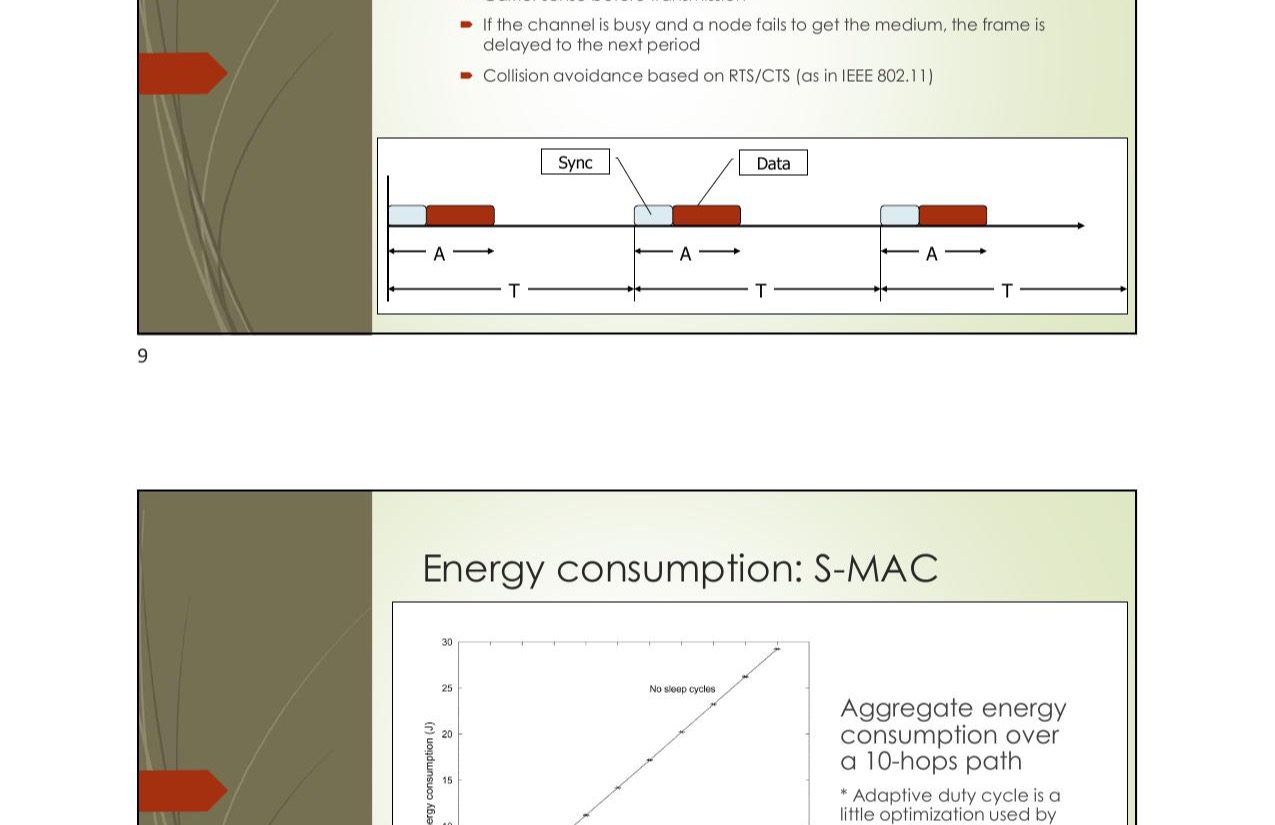
\includegraphics[keepaspectratio]{images/lezione-17-mac-protocols-img-01.jpg}}
\caption{Il frame Sync e Data trasmessi nel periodo di attività.}
\end{figure}

\begin{figure}
\centering
\pandocbounded{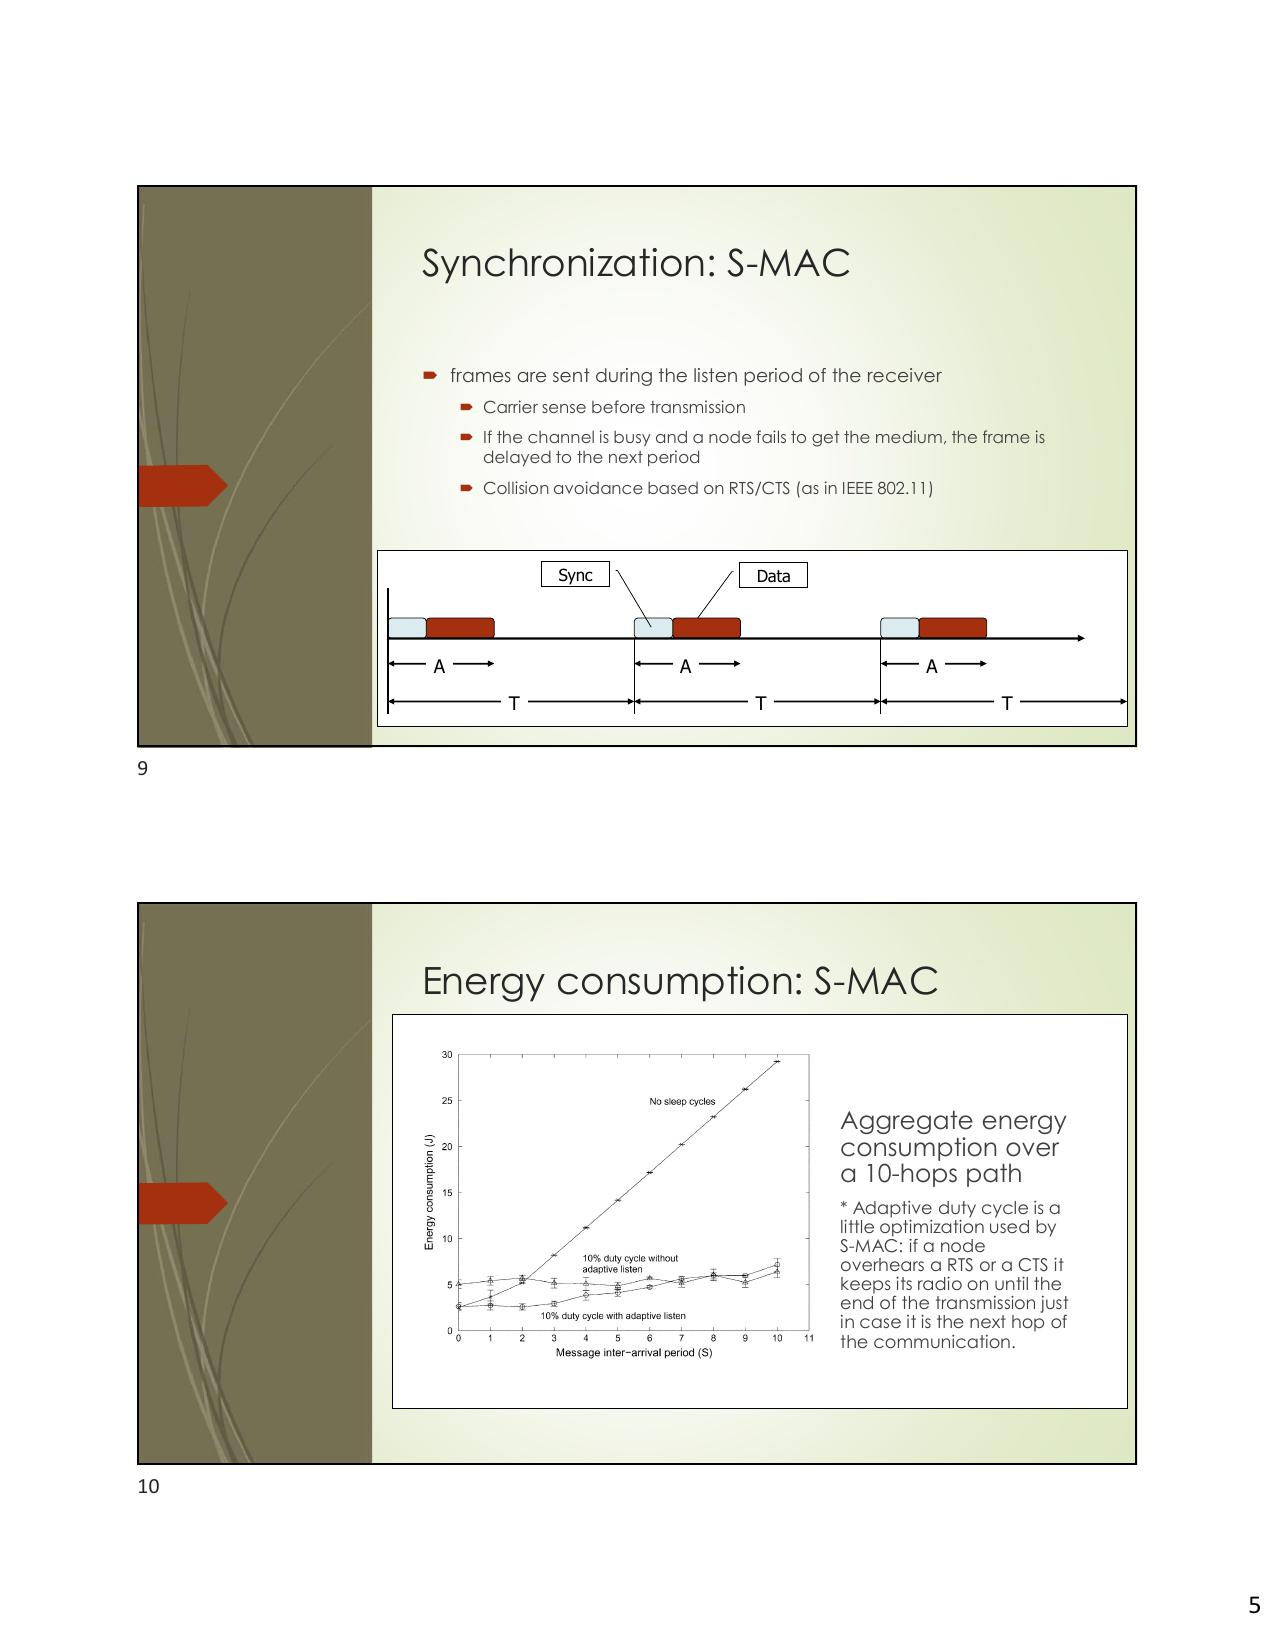
\includegraphics[keepaspectratio]{images/lezione-17-mac-protocols-img-02.jpg}}
\caption{Consumo energetico totale in funzione del traffico.}
\end{figure}

\textbf{Latenza multi-hop e Clock Drift:} La latenza si accumula
(proporzionale a \(n \times T_{listen\_period}\)) se le schedule nei
salti successivi non sono allineate. Per contrastare il clock drift
(deriva hardware), i frame SYNC periodici mantengono i nodi allineati
nel tempo.

\begin{figure}
\centering
\pandocbounded{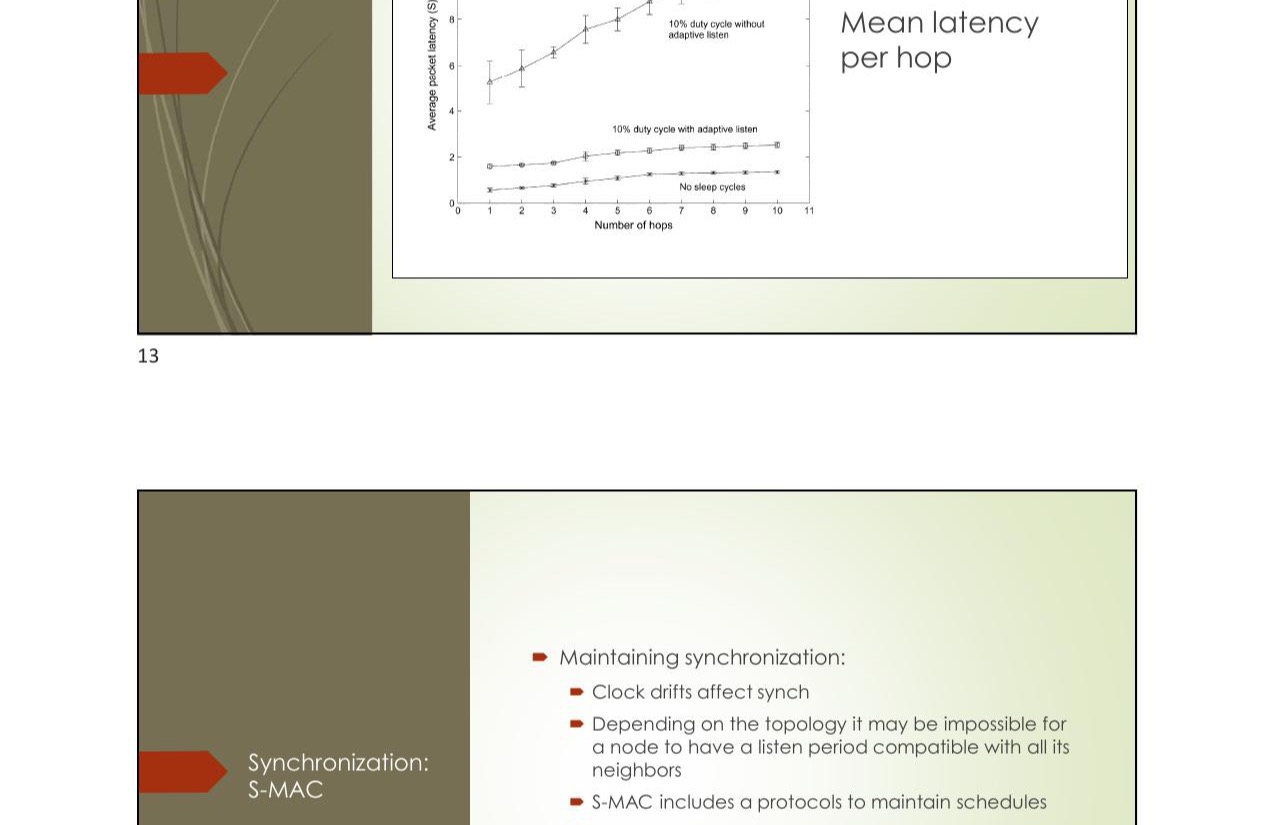
\includegraphics[keepaspectratio,alt={Latenza media per hop in S-MAC}]{images/lezione-17-mac-protocols-img-03.jpg}}
\caption{Latenza media per hop in S-MAC}
\end{figure}

\subsection{Preamble Sampling: B-MAC}\label{preamble-sampling-b-mac}

B-MAC (\emph{Berkeley MAC}) elimina la necessità di coordinazione
temporale sfruttando il \emph{Low-Power Listening} (LPL). Il ricevitore
attiva la radio periodicamente per brevissimi istanti per campionare il
canale. Il mittente, quando deve trasmettere, invia un preambolo molto
lungo (la cui durata deve essere superiore al periodo di sleep del
ricevitore) seguito dal frame dati.

\begin{figure}
\centering
\pandocbounded{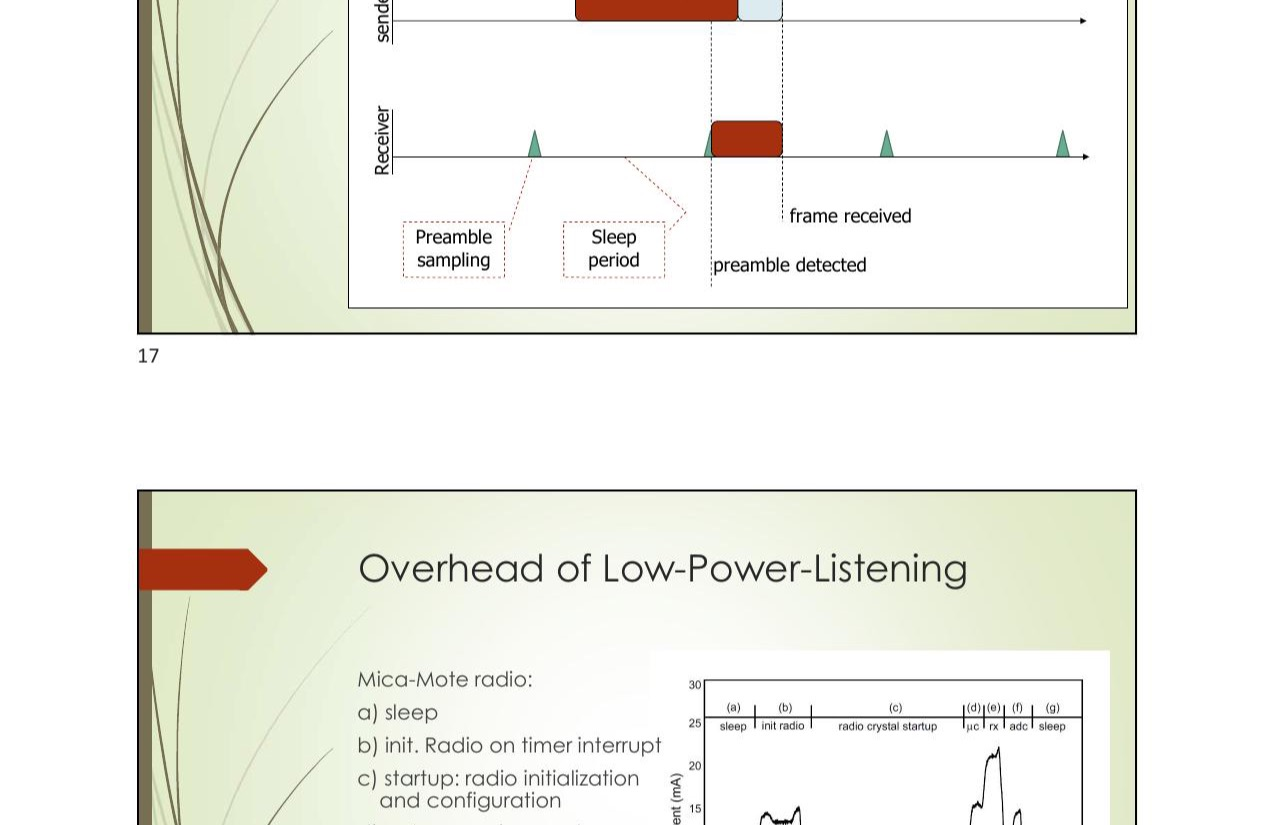
\includegraphics[keepaspectratio,alt={Schema temporale del preamble sampling B-MAC}]{images/lezione-17-mac-protocols-img-04.jpg}}
\caption{Schema temporale del preamble sampling B-MAC}
\end{figure}

\begin{figure}
\centering
\pandocbounded{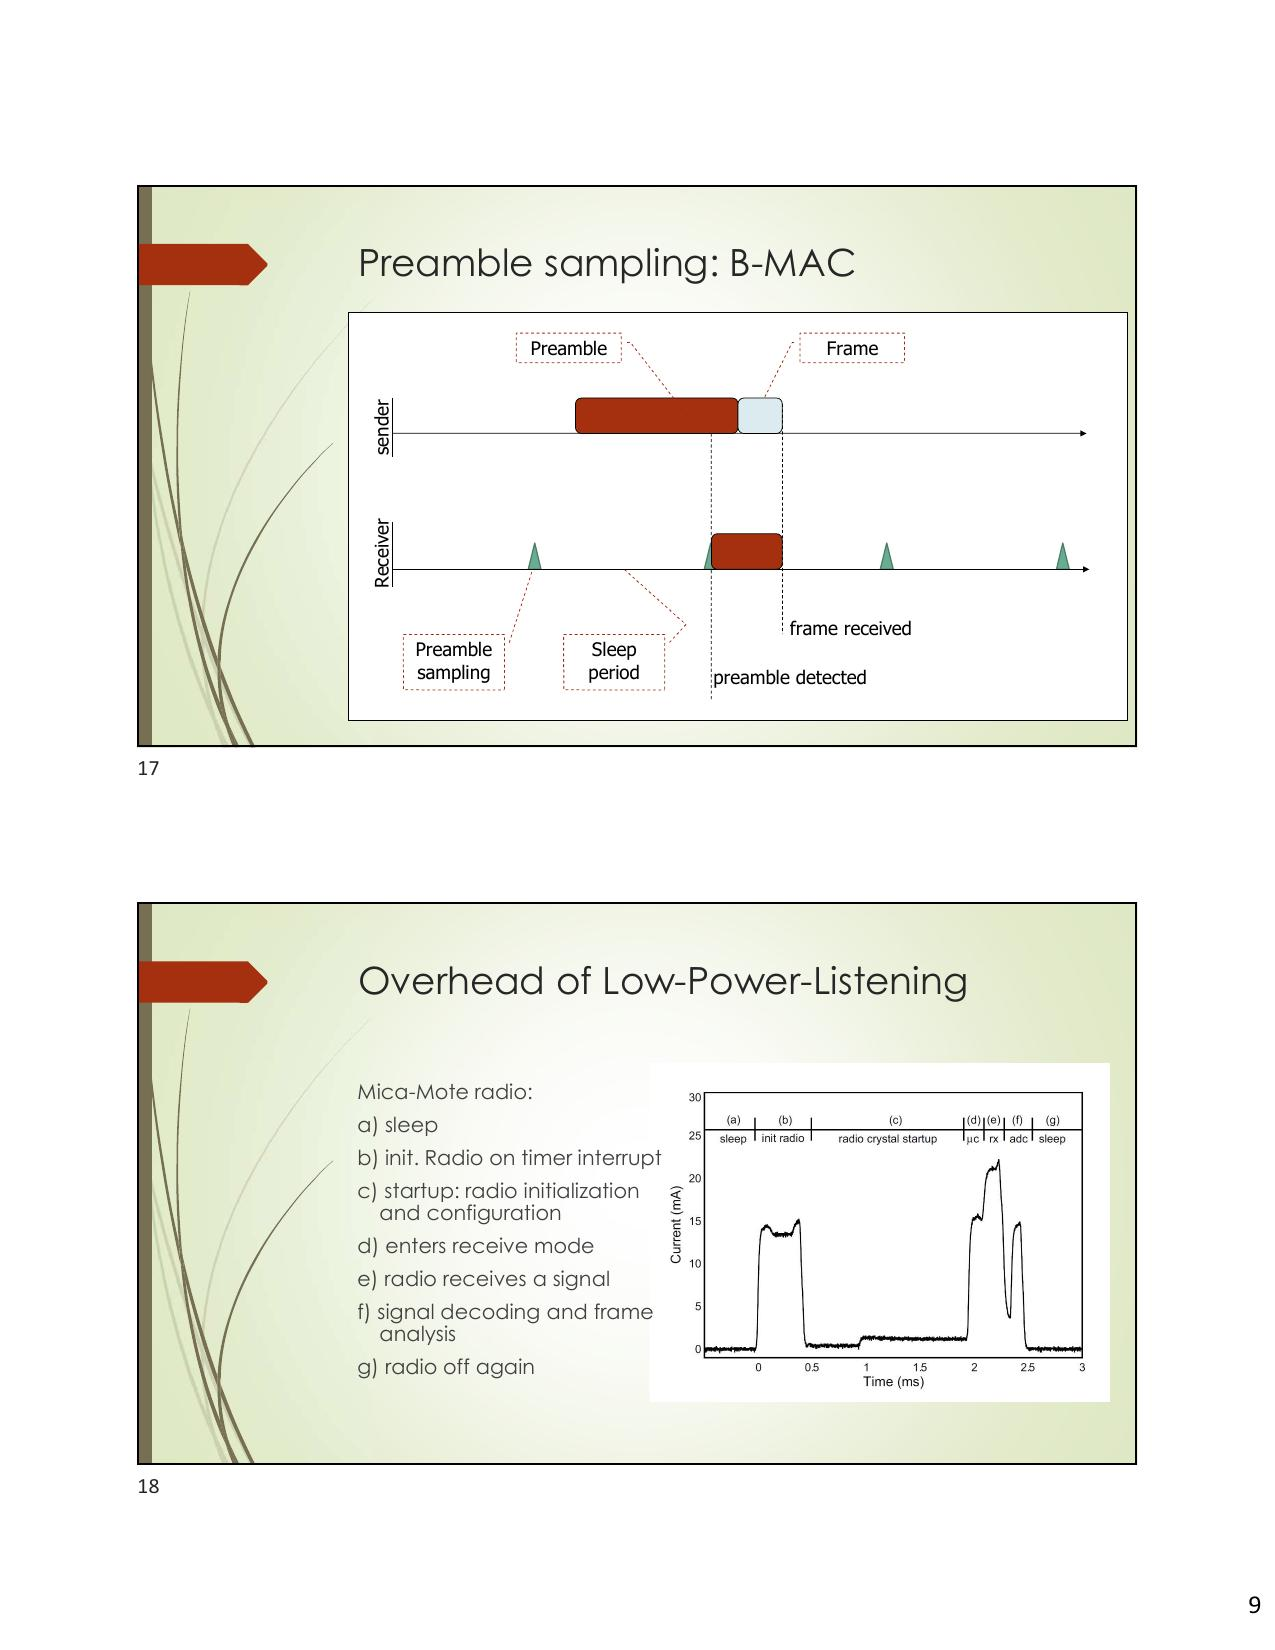
\includegraphics[keepaspectratio,alt={Profilo di corrente del radio Mica-Mote durante il ciclo LPL}]{images/lezione-17-mac-protocols-img-05.jpg}}
\caption{Profilo di corrente del radio Mica-Mote durante il ciclo LPL}
\end{figure}

\textbf{Modello energetico}: Siano: - \(f_d\) = frequenza di
trasmissione dei dati (Hz) - \(f_c\) = frequenza di campionamento del
preambolo - \(p_t, p_r, p_i\) = potenza in trasmissione, ricezione,
idle.

Per il \textbf{trasmittente}, il duty cycle è:
\[DC_{data} = f_d \cdot (t_{preamble} + t_{frame})\]
\[DC_{check} = f_d \cdot t_{check}\] L'energia consumata in \(t\)
secondi:
\[E_T(t) = t \left[ p_t \cdot DC_{data} + p_r \cdot DC_{check} + p_i \cdot (1 - DC_{data} - DC_{check}) \right]\]

Per il \textbf{ricevitore}:
\[DC_{data} = f_c \cdot (t_{listen} + t_{data})\]
\[DC_{check} = f_c \cdot t_{check}\]
\[E_R(t) = t \left[ p_r \cdot DC_{data} + p_r \cdot DC_{check} + p_i \cdot (1 - DC_{data} - DC_{check}) \right]\]

Il preambolo lungo costa molta energia in trasmissione, ma garantisce
grandissimi risparmi per tutti i ricevitori in ascolto, che necessitano
di campionamenti piccolissimi. B-MAC ha un solo parametro di setup:
l'intervallo di check.

\subsection{Evoluzioni: X-MAC e
BoX-MAC}\label{evoluzioni-x-mac-e-box-mac}

\textbf{X-MAC}: Ottimizza il costo in trasmissione dividendo il lungo
preambolo in brevi frame ripetuti contenenti l'ID del destinatario.
Quando il ricevitore si sveglia e legge il proprio ID, interrompe
immediatamente il trasmettitore inviando un ACK precoce, spingendolo a
inviare il frame effettivo e risparmiando energia.

\begin{figure}
\centering
\pandocbounded{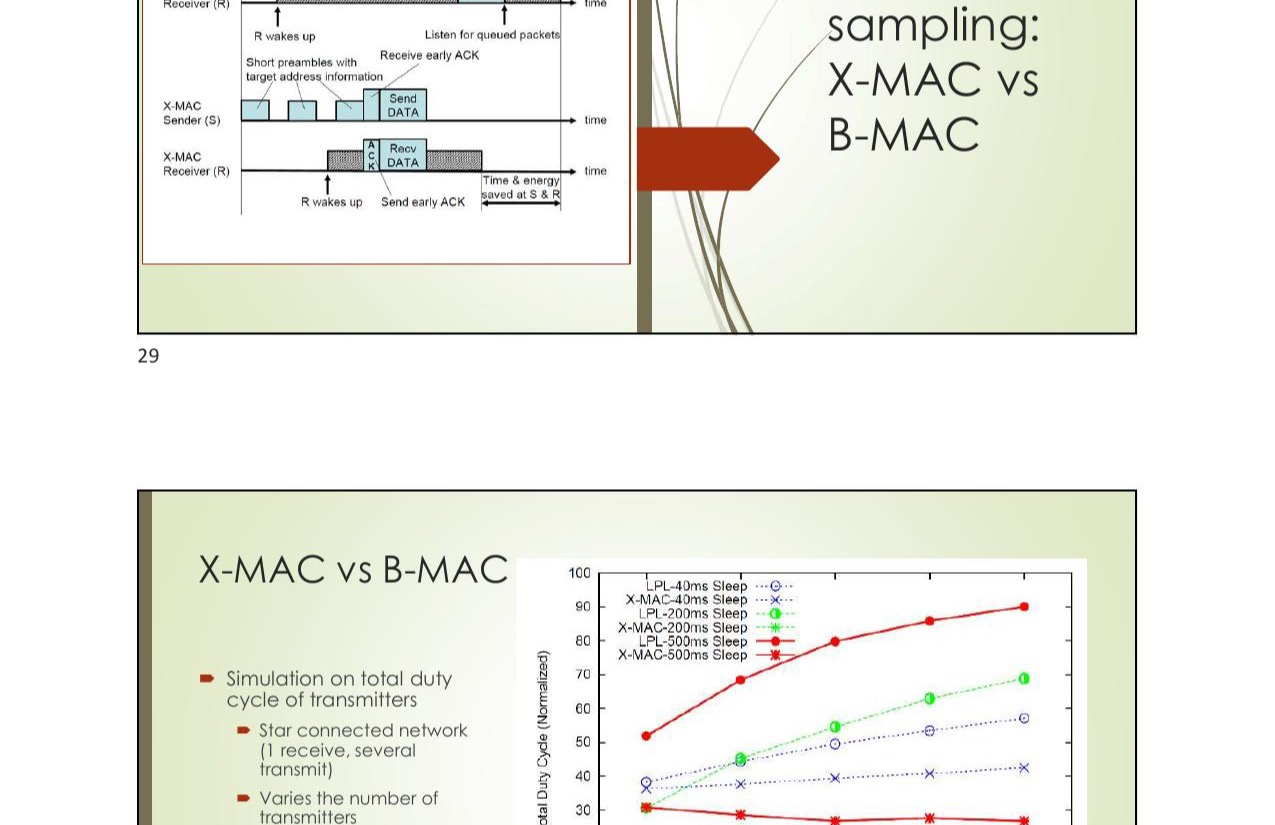
\includegraphics[keepaspectratio,alt={Confronto temporale X-MAC vs B-MAC}]{images/lezione-17-mac-protocols-img-06.jpg}}
\caption{Confronto temporale X-MAC vs B-MAC}
\end{figure}

\begin{figure}
\centering
\pandocbounded{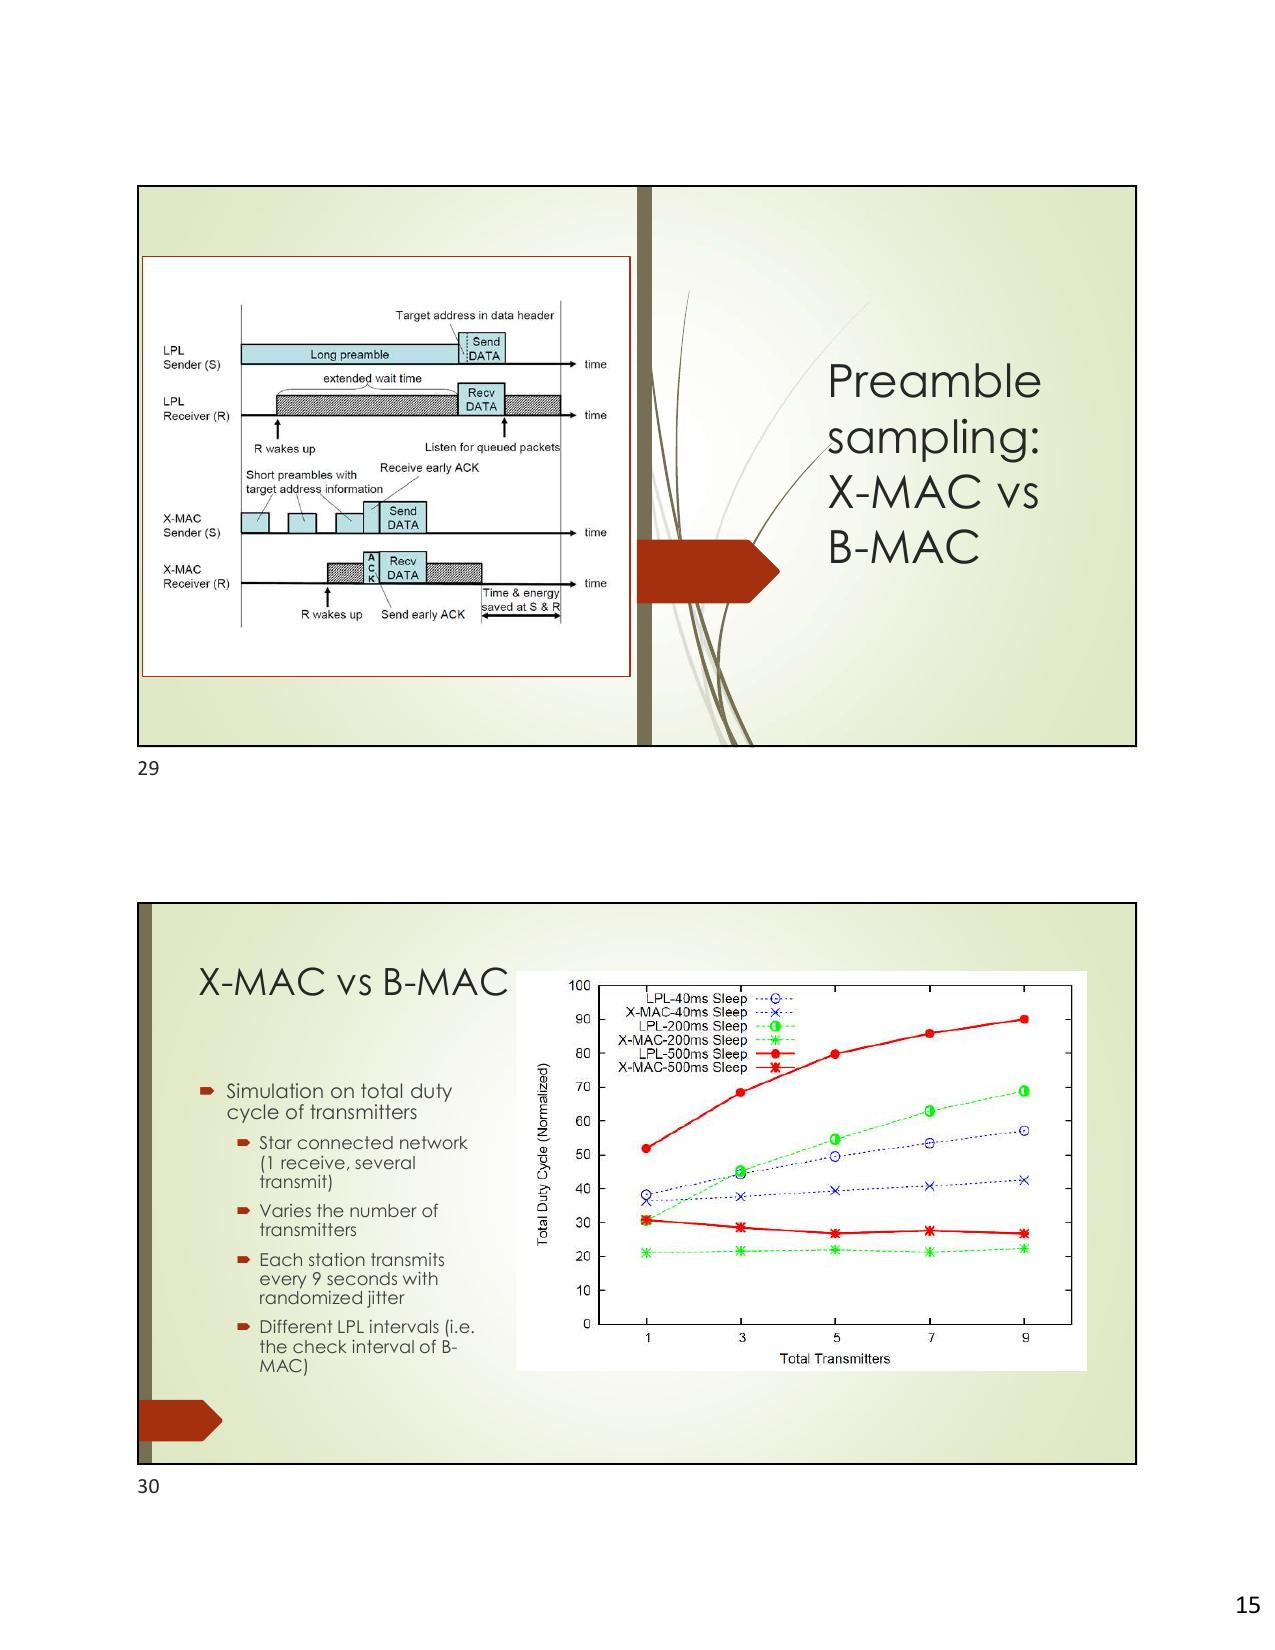
\includegraphics[keepaspectratio,alt={Duty cycle totale trasmittenti: X-MAC vs B-MAC al variare del numero di nodi}]{images/lezione-17-mac-protocols-img-07.jpg}}
\caption{Duty cycle totale trasmittenti: X-MAC vs B-MAC al variare del
numero di nodi}
\end{figure}

\textbf{BoX-MAC}: Un'ulteriore evoluzione in cui il ``preambolo''
diventa il frame dati stesso, ripetuto in loop. Il ricevitore intercetta
un frammento, aspetta l'inizio della replica successiva, la riceve per
intero e manda l'ACK per fermare il mittente. È eccellente per reti di
sensori che scambiano frame molto leggeri.

\begin{figure}
\centering
\pandocbounded{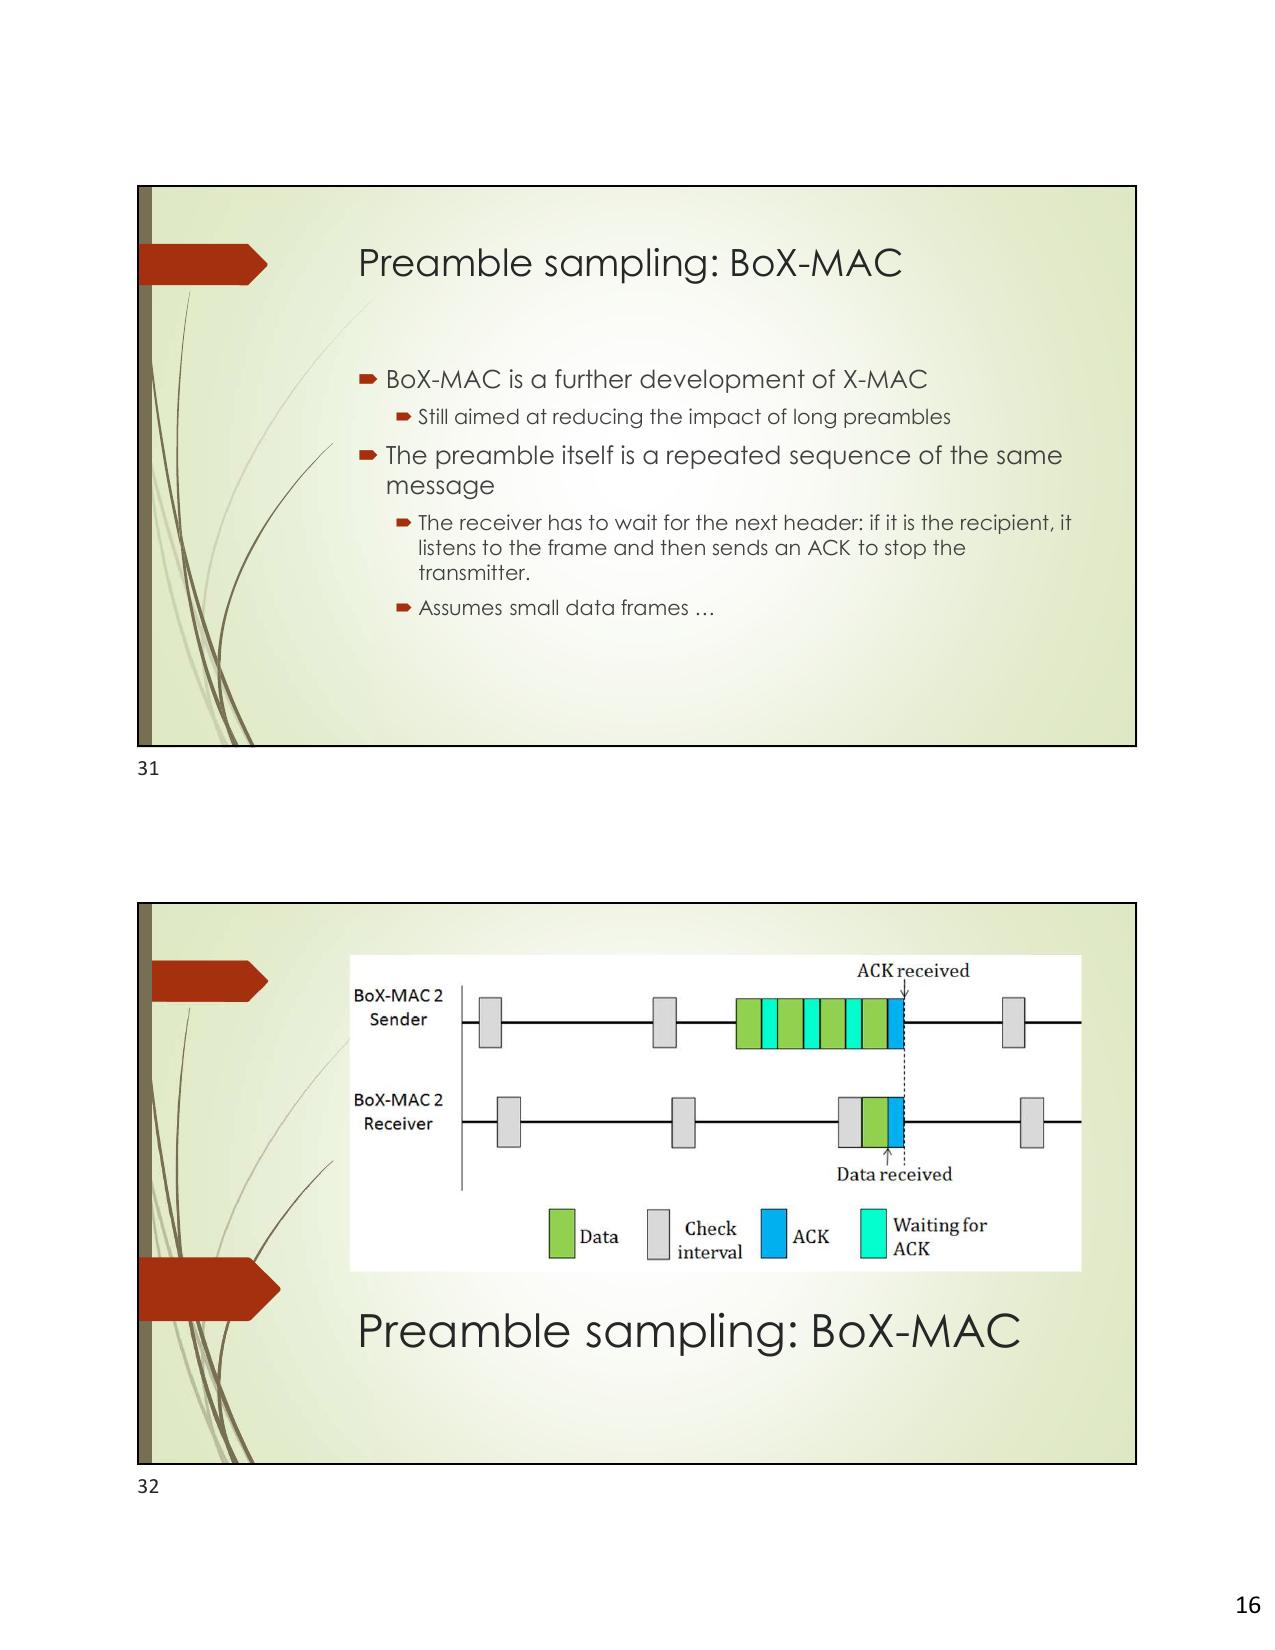
\includegraphics[keepaspectratio,alt={Diagramma temporale BoX-MAC}]{images/lezione-17-mac-protocols-img-08.jpg}}
\caption{Diagramma temporale BoX-MAC}
\end{figure}

\begin{figure}
\centering
\pandocbounded{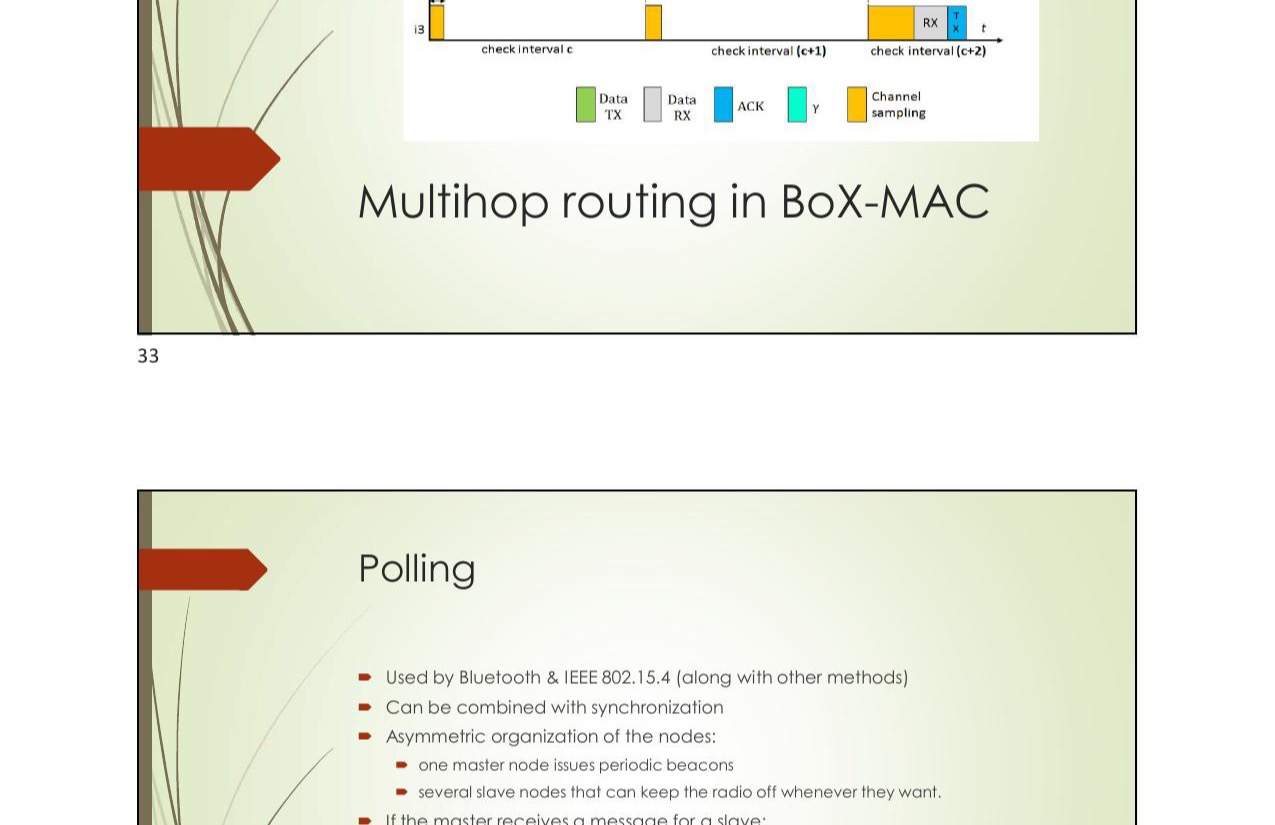
\includegraphics[keepaspectratio,alt={Routing multi-hop in BoX-MAC}]{images/lezione-17-mac-protocols-img-09.jpg}}
\caption{Routing multi-hop in BoX-MAC}
\end{figure}

\subsection{Polling}\label{polling}

Tipico di Bluetooth e \textbf{IEEE 802.15.4} (combinato con la
sincronizzazione). L'architettura è asimmetrica: un nodo master annuncia
messaggi pendenti tramite \emph{beacon}, i nodi slave possono tenere la
radio spenta a piacimento e si svegliano per prelevare il messaggio dal
master inviando una richiesta esplicita.

\begin{center}\rule{0.5\linewidth}{0.5pt}\end{center}

\section{2. Lo Standard IEEE 802.15.4 (Lezione
18)}\label{lo-standard-ieee-802.15.4-lezione-18}

Fornisce le specifiche del \textbf{Physical layer} e del \textbf{MAC
layer} per reti \textbf{LR-WPAN} (Low-Rate Wireless Personal Area
Network). Opera con dispositivi a risorse limitate, garantendo consumi
ridotti, coesistenza con Wi-Fi (802.11) e Bluetooth (802.15.1).

\subsection{Physical Layer}\label{physical-layer}

Opera in bande libere da licenza: \textbar{} Banda \textbar{} Regione
\textbar{} Data rate \textbar{} Canali \textbar{}
\textbar---\textbar---\textbar---\textbar---\textbar{} \textbar{}
868--868.6 MHz \textbar{} Europa \textbar{} 20 kbps \textbar{} 1 (canale
0) \textbar{} \textbar{} 902--928 MHz \textbar{} Nord America \textbar{}
40 kbps \textbar{} 10 (canali 1--10) \textbar{} \textbar{} 2400--2483.5
MHz \textbar{} Mondiale \textbar{} 250 kbps \textbar{} 16 (canali
11--26) \textbar{}

Eroga \emph{Data Service} per ricezione/trasmissione e \emph{Management
Service} per funzioni fisiche: - \textbf{Energy Detection (ED)}: Misura
l'energia sul canale (su una finestra di 8 simboli) con soglia di 10 dB
sopra la sensibilità radio. - \textbf{Link Quality Indicator (LQI)}:
Stima della qualità del frame ricevuto per alimentare le logiche di
routing. - \textbf{Clear Channel Assessment (CCA)}: Verifica se il
canale è libero tramite 3 modalità (tramite ED, tramite Carrier Sense, o
combinazione logica).

\begin{figure}
\centering
\pandocbounded{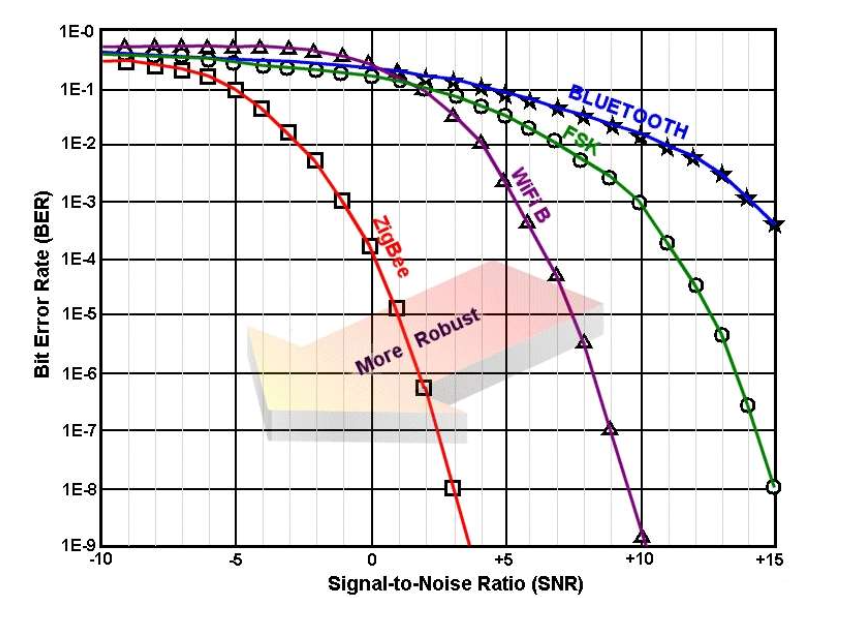
\includegraphics[keepaspectratio]{images/Pasted-image-20260408111308.png}}
\caption{L'ottima resistenza di 802.15.4 al rumore (BER vs SNR).}
\end{figure}

\textbf{Struttura della PPDU} (PHY Protocol Data Unit): - \emph{SHR}:
Synchronization Header (preambolo e SFD). - \emph{PHR}: PHY Header
(lunghezza, max 127 byte). - \emph{PHY Payload}: PSDU.

\begin{figure}
\centering
\pandocbounded{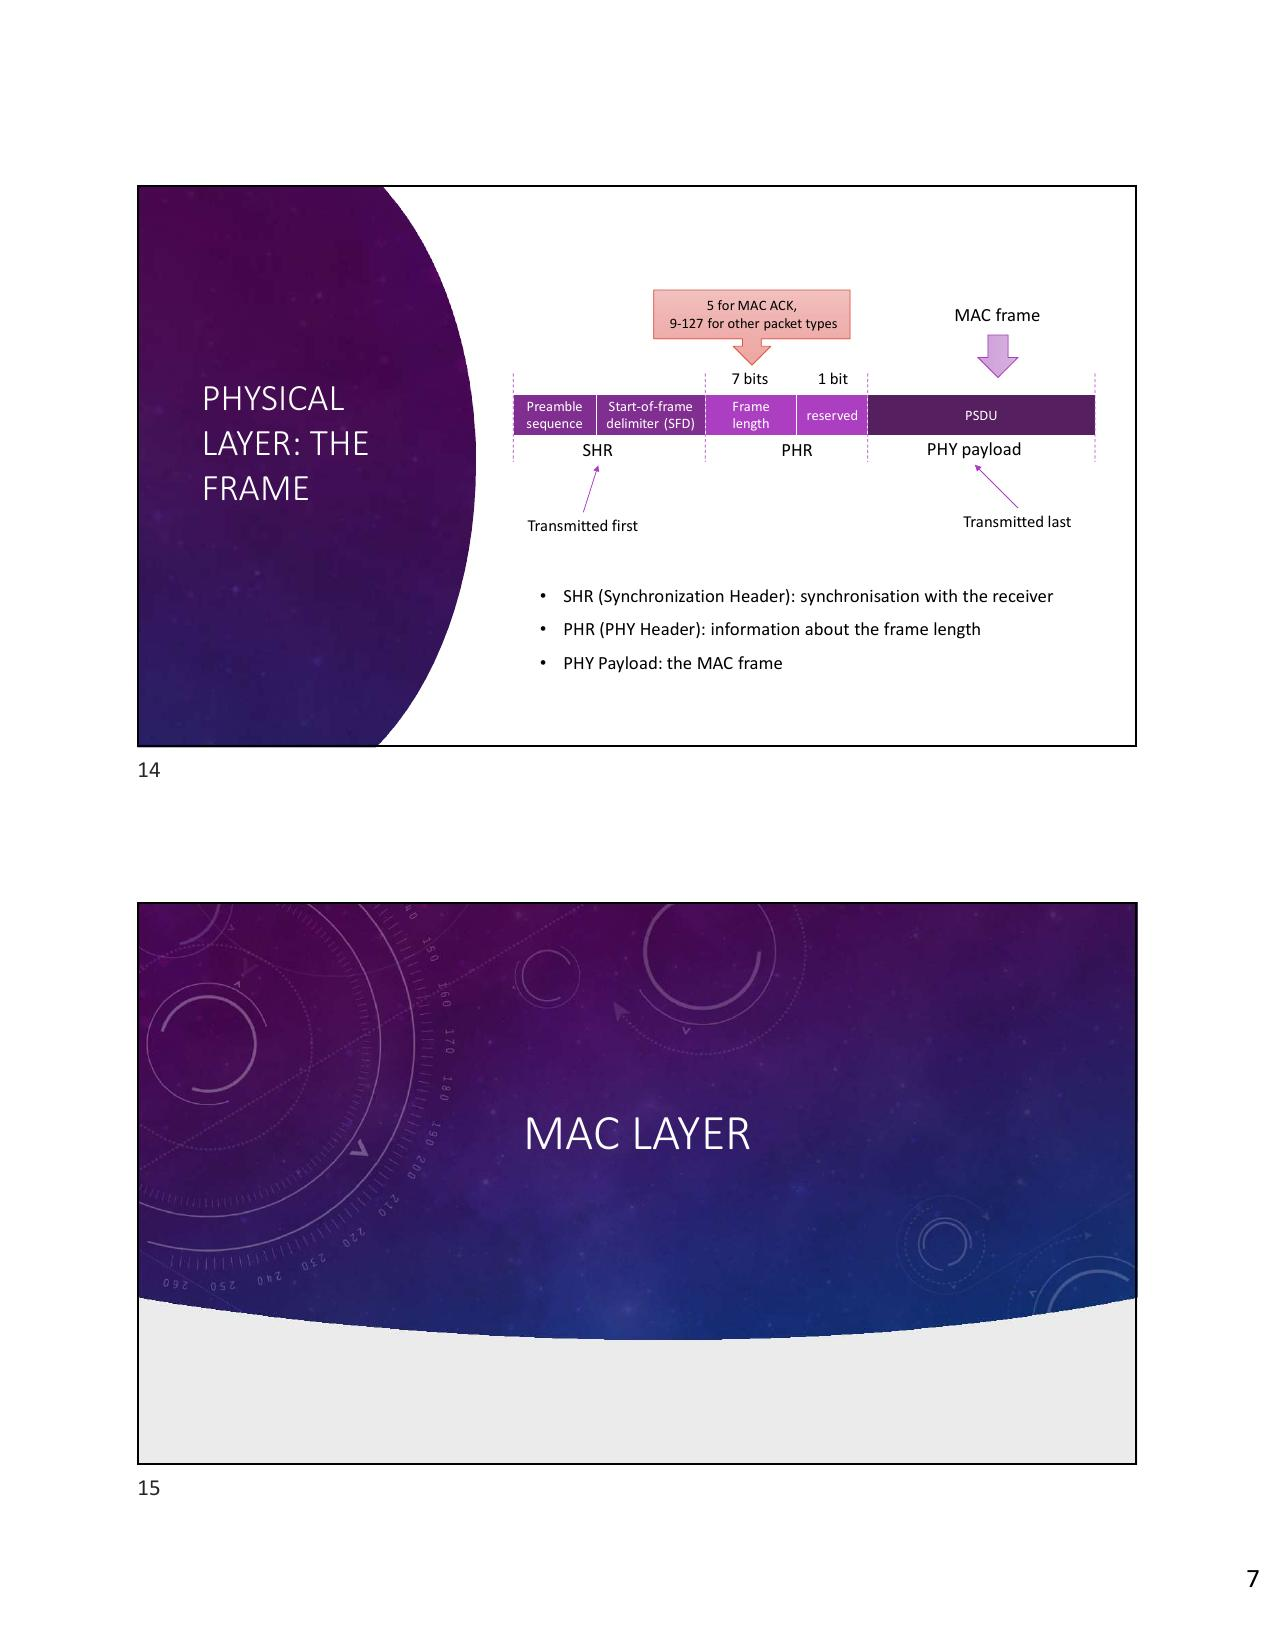
\includegraphics[keepaspectratio,alt={Struttura della PPDU IEEE 802.15.4}]{images/lezione-18-the-ieee-802-15-4-standard-img-01.jpg}}
\caption{Struttura della PPDU IEEE 802.15.4}
\end{figure}

\subsection{MAC Layer: Dispositivi e
Topologie}\label{mac-layer-dispositivi-e-topologie}

Esistono due classi di nodi: - \textbf{RFD (Reduced Function Device)}:
Logica minima, destinato agli end-device (sensori). Può associarsi a un
solo nodo padre FFD. - \textbf{FFD (Full Function Device)}: Logica MAC
completa. Può agire da Router, da \emph{PAN Coordinator} (che crea la
rete) o da end-device generico.

Le topologie supportate sono \textbf{Stella} (Coordinator al centro,
comunicazioni dirette solo verso di lui) e \textbf{Peer-to-Peer} (FFD
connessi in mesh/albero, RFD appesi come foglie).
\pandocbounded{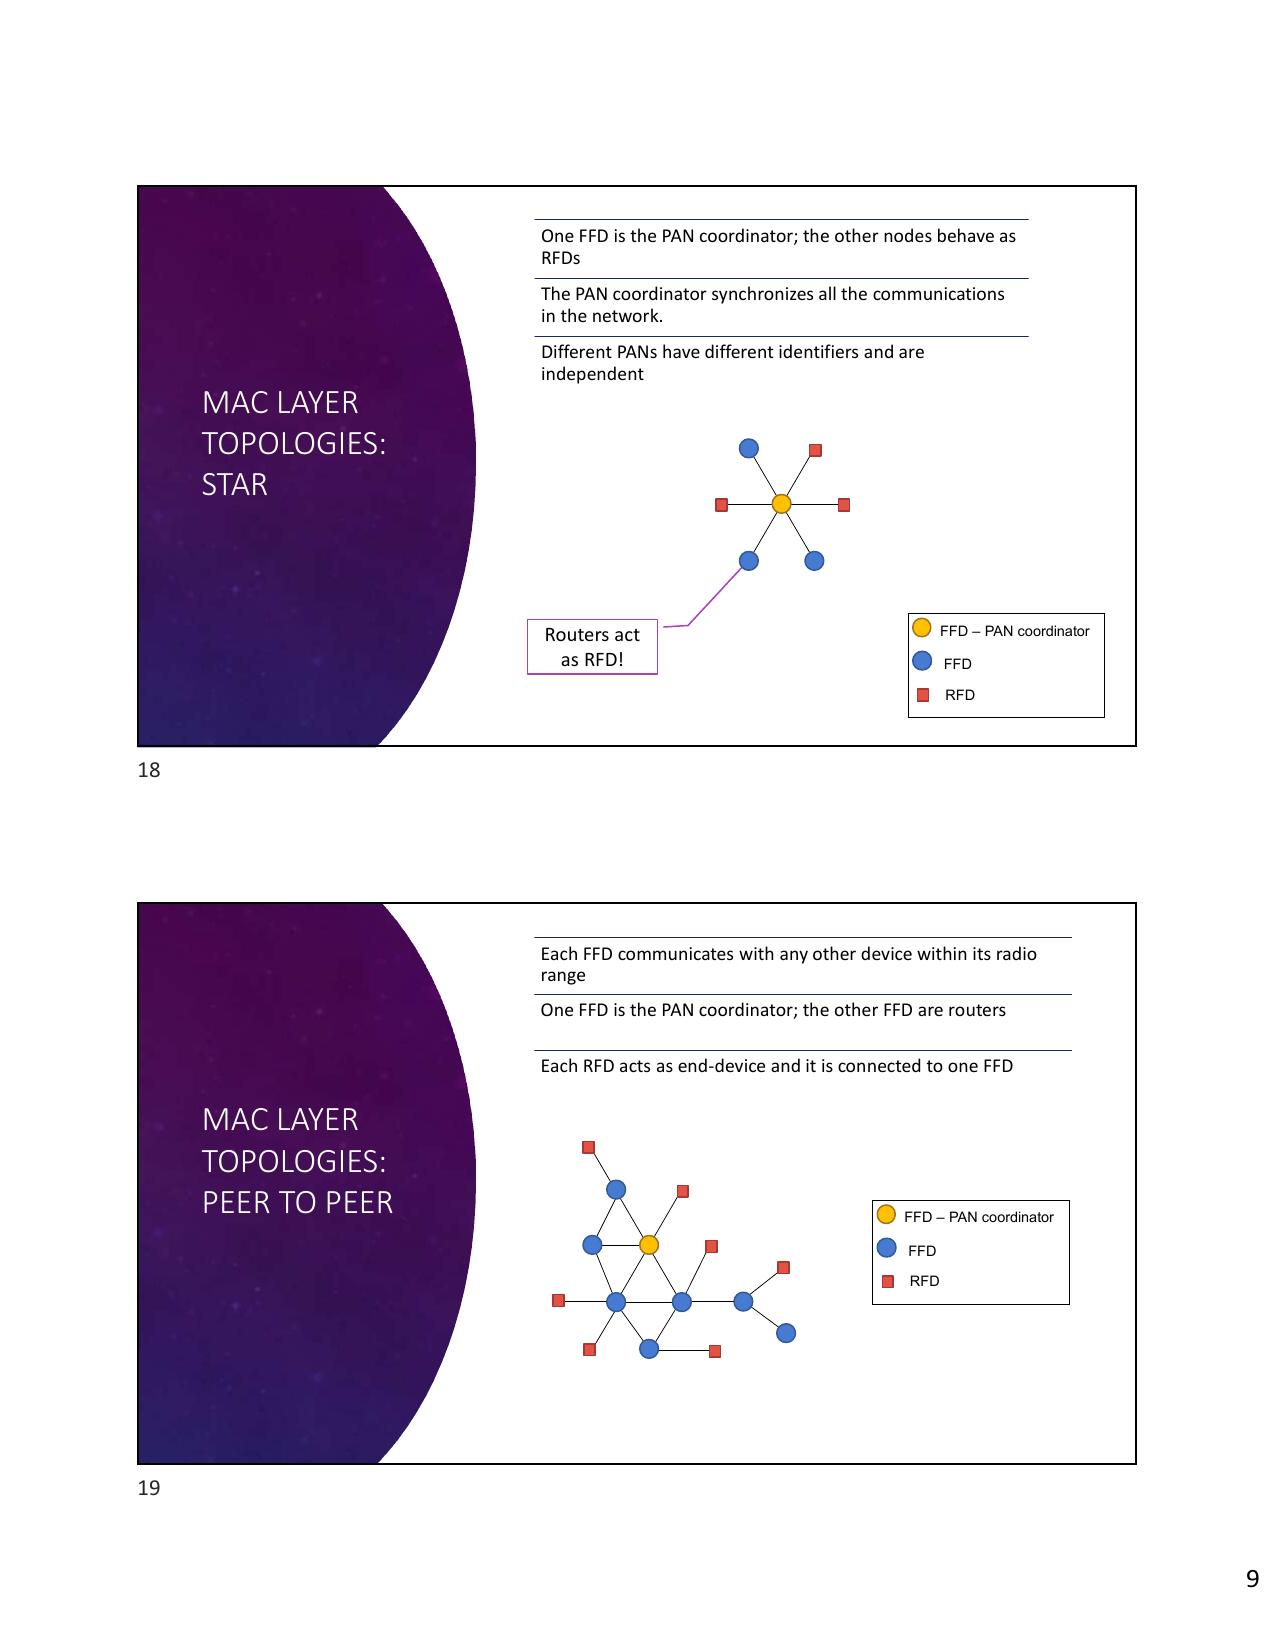
\includegraphics[keepaspectratio,alt={Topologia Star IEEE 802.15.4}]{images/lezione-18-the-ieee-802-15-4-standard-img-02.jpg}}

\begin{figure}
\centering
\pandocbounded{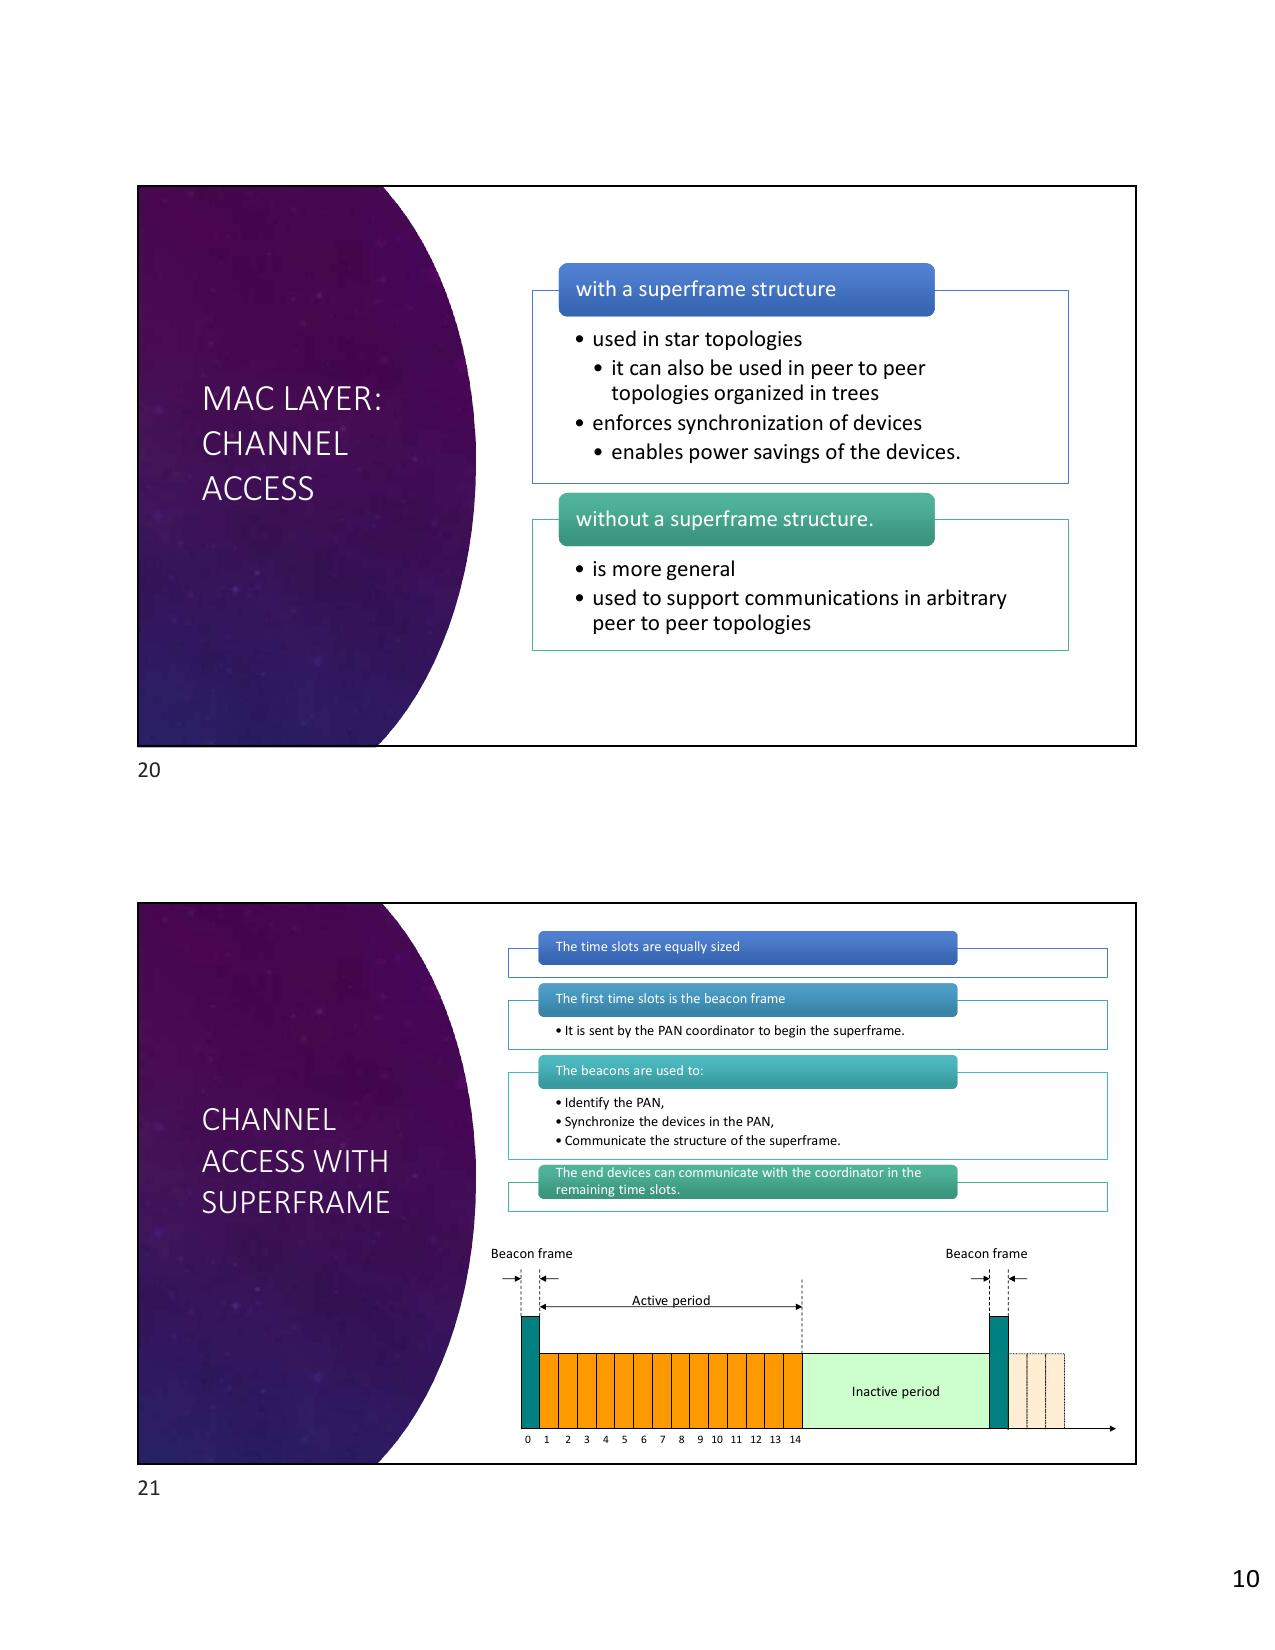
\includegraphics[keepaspectratio,alt={Topologia Peer-to-Peer IEEE 802.15.4}]{images/lezione-18-the-ieee-802-15-4-standard-img-03.jpg}}
\caption{Topologia Peer-to-Peer IEEE 802.15.4}
\end{figure}

\subsection{Accesso al Canale e
Superframe}\label{accesso-al-canale-e-superframe}

\textbf{Modalità Beacon-Enabled}: Il coordinatore trasmette beacon
periodici definendo un \textbf{Superframe}. Il superframe è diviso in
periodo attivo (in cui si comunica) e inattivo (tutti in sleep). Il
periodo attivo contiene fino a 16 slot suddivisi in: - \textbf{CAP
(Contention Access Period)}: accesso tramite \emph{slotted CSMA-CA}. -
\textbf{CFP (Contention Free Period)}: opzionale, slot garantiti
\textbf{GTS} assegnati a dispositivi specifici per determinismo
temporale.

\begin{calloutwarning}{Il CAP non può essere eliminato}

Il CAP è indispensabile per gestire messaggi asincroni (associazioni,
richieste GTS) e deve esistere anche se è presente il CFP.

\end{calloutwarning}

\begin{figure}
\centering
\pandocbounded{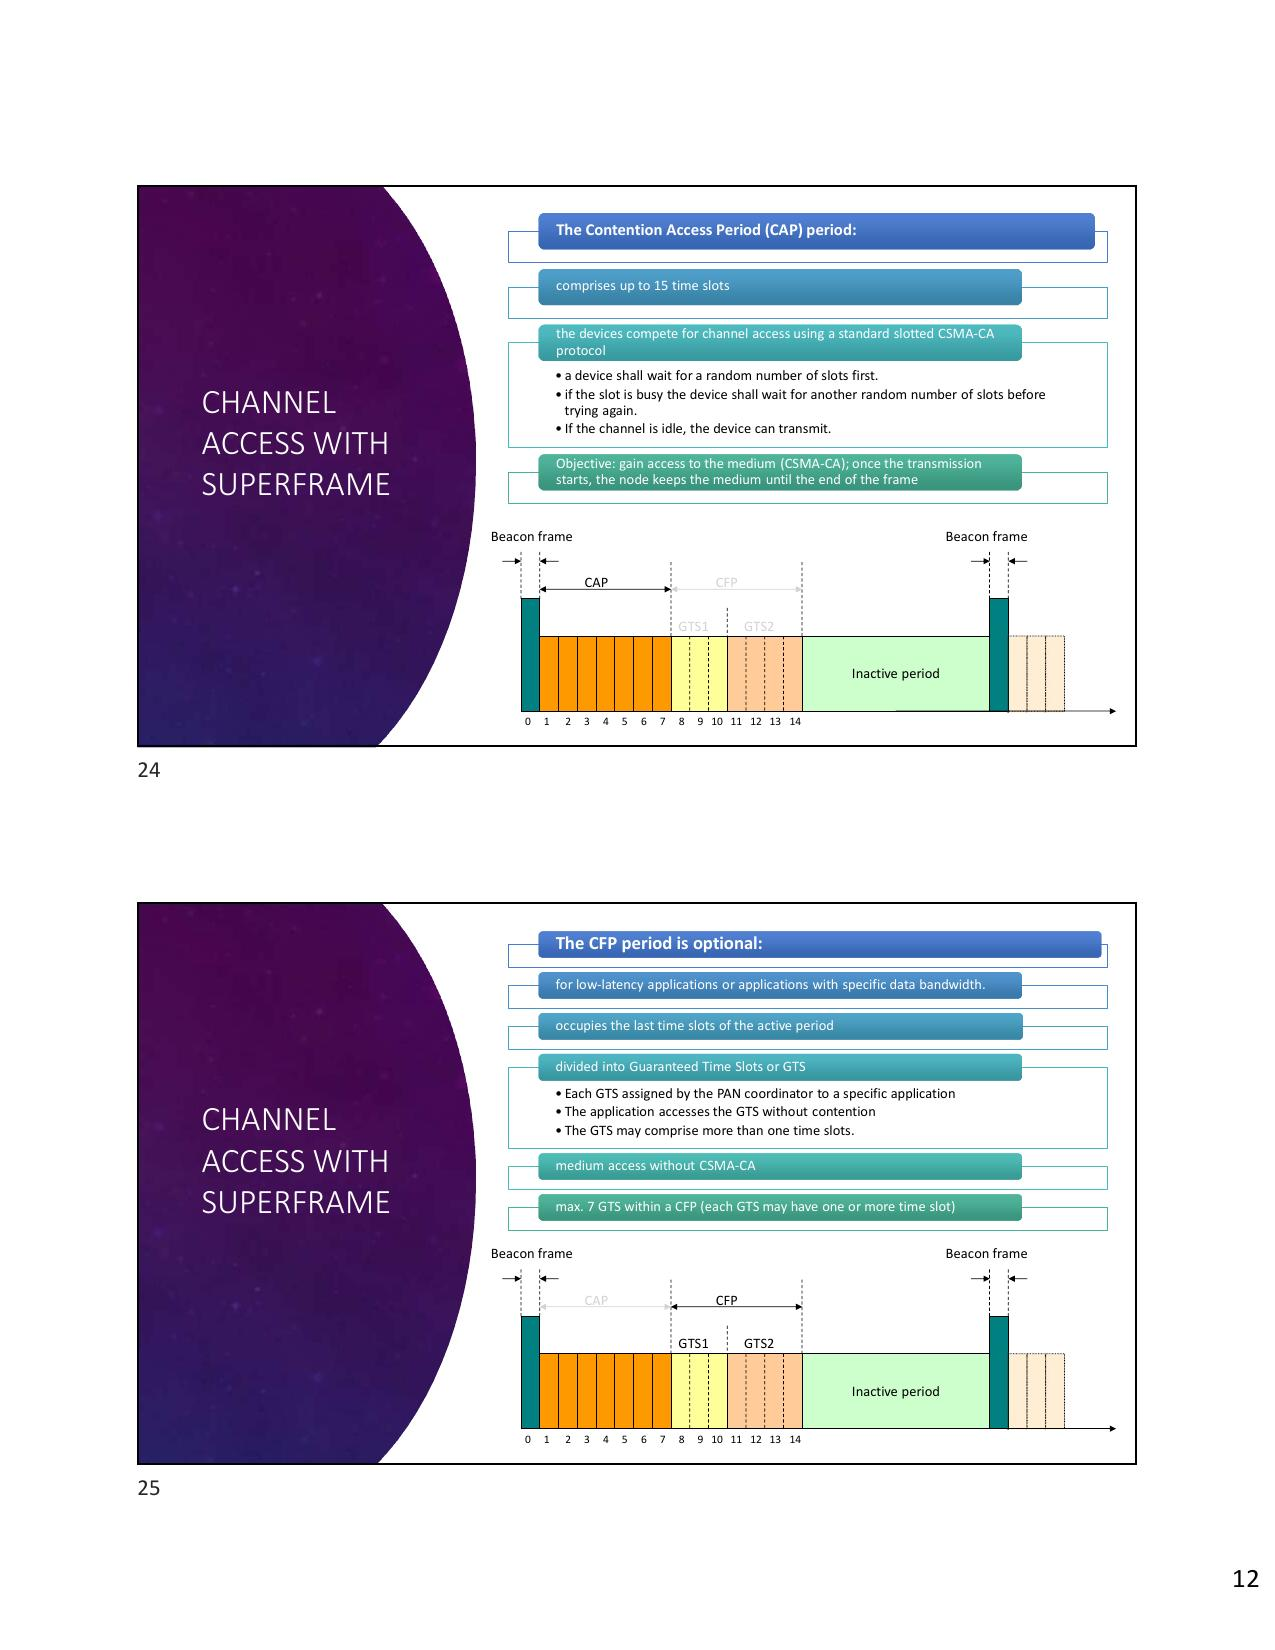
\includegraphics[keepaspectratio,alt={Struttura del superframe CAP e CFP}]{images/lezione-18-the-ieee-802-15-4-standard-img-04.jpg}}
\caption{Struttura del superframe CAP e CFP}
\end{figure}

\textbf{Modalità Non Beacon-Enabled}: Nessun superframe. Usa
\textbf{unslotted CSMA-CA}. I coordinatori devono restare sempre accesi.
L'end-device preleva dati tramite polling al coordinatore.

\subsection{Associazione e Sicurezza}\label{associazione-e-sicurezza}

Il MAC fornisce una suite di primitive: \texttt{DATA},
\texttt{ASSOCIATE}, \texttt{SCAN}, \texttt{GTS}, \texttt{POLL}.
L'associazione si basa su: Scansione (\texttt{SCAN}), richiesta
dell'end-device al PAN Coordinator (\texttt{ASSOCIATE.request}),
accettazione del coordinatore con assegnazione di short address a 16-bit
(\texttt{ASSOCIATE.response} via polling indiretto).

\begin{figure}
\centering
\pandocbounded{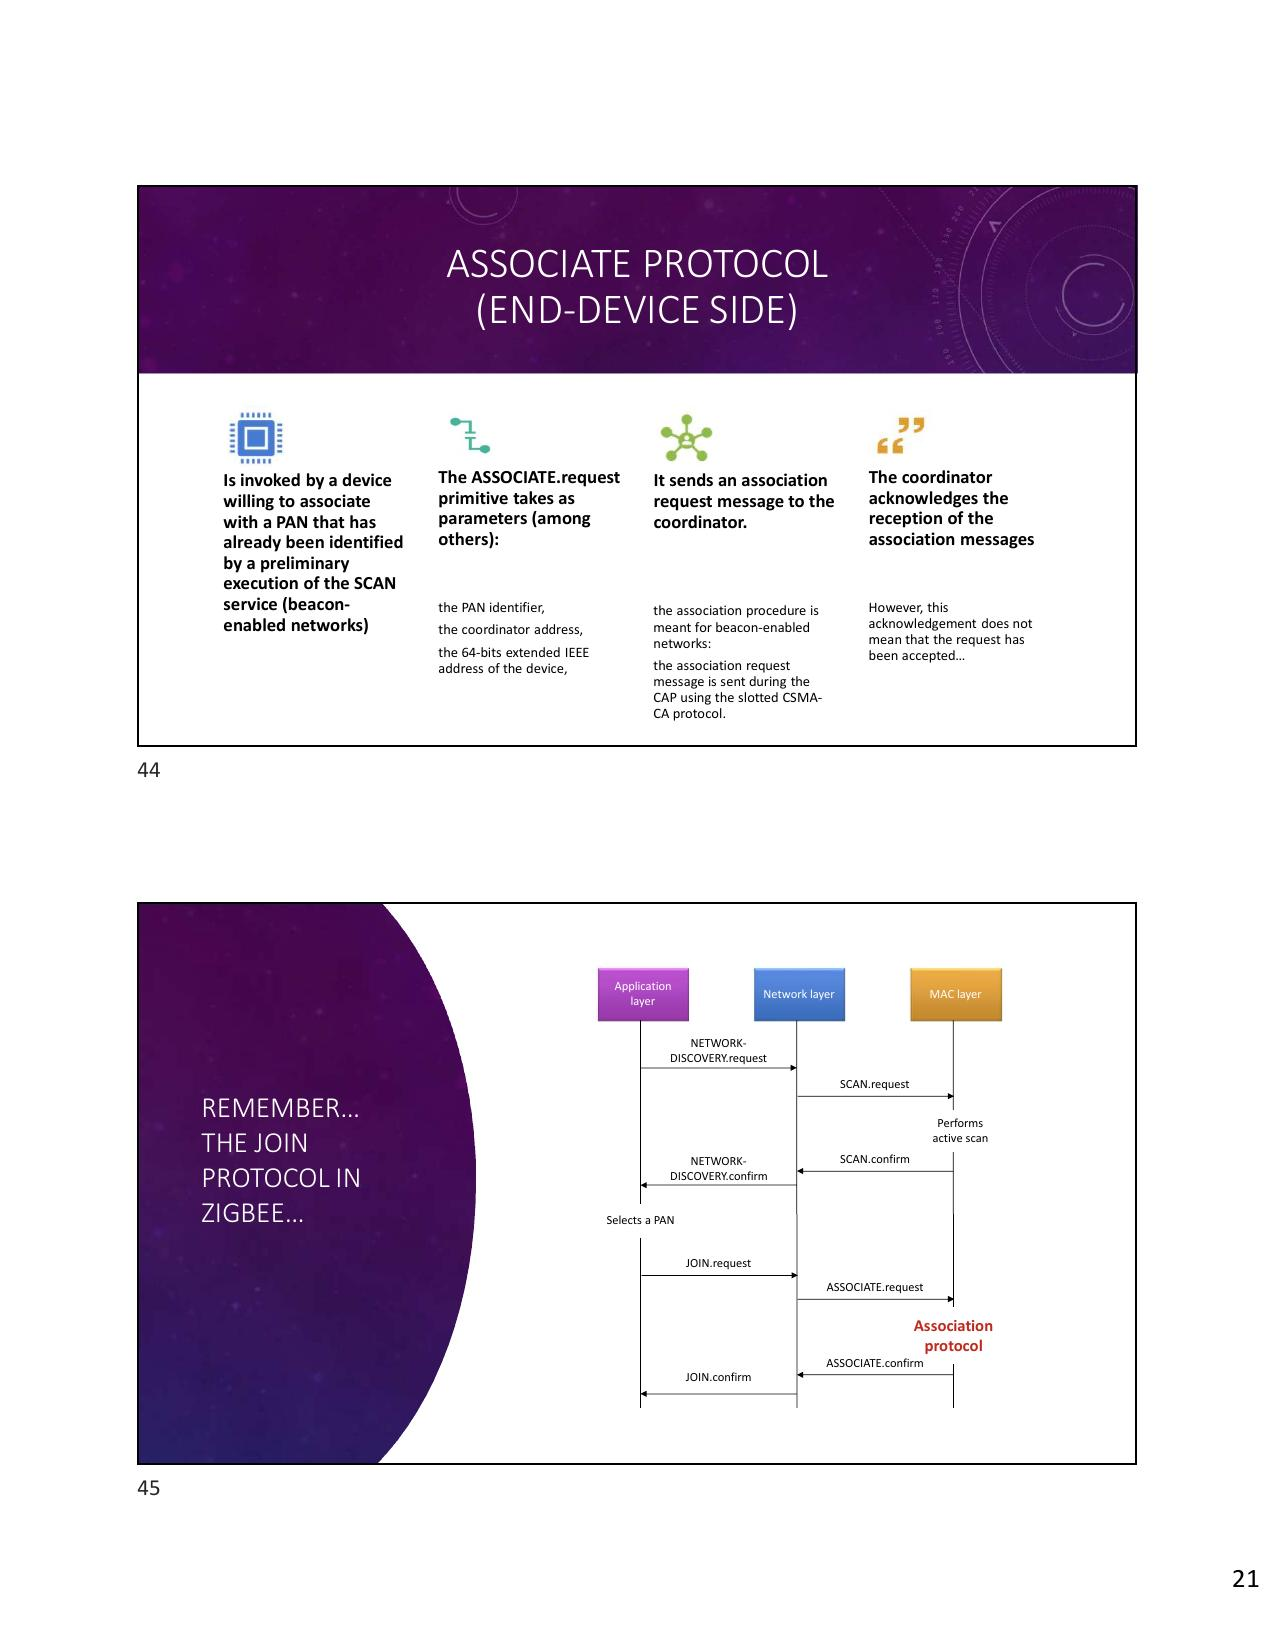
\includegraphics[keepaspectratio,alt={Diagramma flusso MAC Data Service e protocollo di associazione ZigBee}]{images/lezione-18-the-ieee-802-15-4-standard-img-05.jpg}}
\caption{Diagramma flusso MAC Data Service e protocollo di associazione
ZigBee}
\end{figure}

\begin{figure}
\centering
\pandocbounded{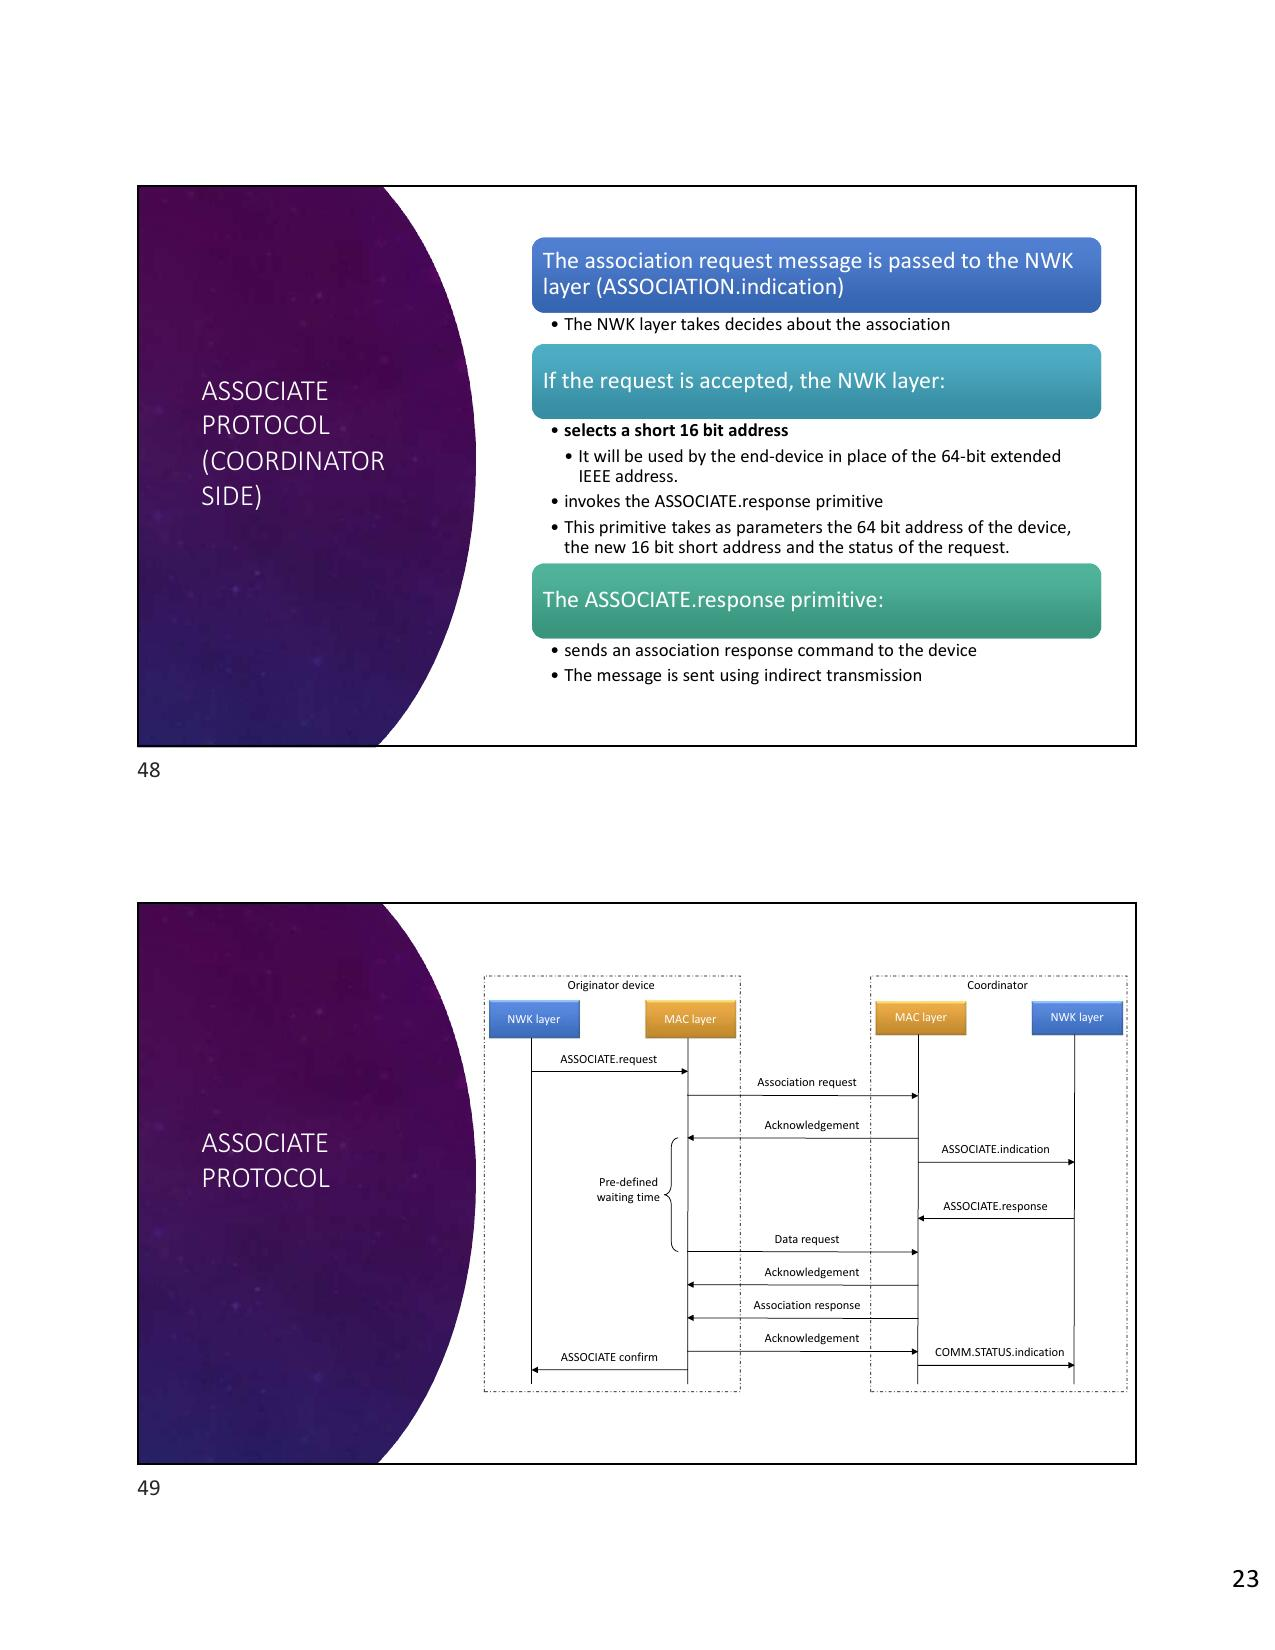
\includegraphics[keepaspectratio,alt={Diagramma di sequenza del protocollo ASSOCIATE IEEE 802.15.4}]{images/lezione-18-the-ieee-802-15-4-standard-img-06.jpg}}
\caption{Diagramma di sequenza del protocollo ASSOCIATE IEEE 802.15.4}
\end{figure}

A livello MAC è integrato il supporto base per la sicurezza (chiavi
simmetriche fornite dal network layer): controllo accessi, cifratura
dati (link o group key), integrità e ``Sequential Freshness'' per
evitare attacchi di replay.

\begin{center}\rule{0.5\linewidth}{0.5pt}\end{center}

\section{3. Lo Standard ZigBee: Network Layer (Lezioni
9)}\label{lo-standard-zigbee-network-layer-lezioni-9}

ZigBee è il protocollo delle reti IoT concepito dalla \emph{ZigBee
Alliance} su basi IEEE 802.15.4, offrendo self-healing, basso costo,
lunga durata batterie e scalabilità. Costruisce sopra PHY e MAC i propri
\textbf{Network (NWK)} e \textbf{Application Layer}.

\pandocbounded{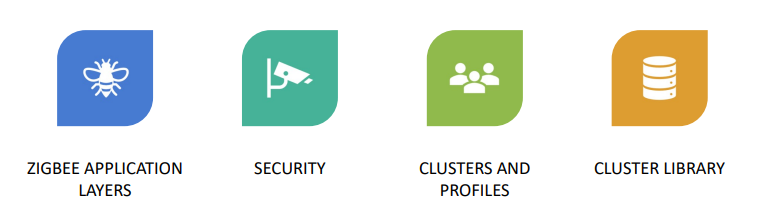
\includegraphics[keepaspectratio]{images/Pasted-image-20260309111850.png}}

\pandocbounded{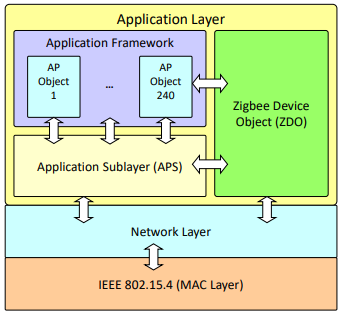
\includegraphics[keepaspectratio]{images/Pasted-image-20260309111918.png}}

\begin{figure}
\centering
\pandocbounded{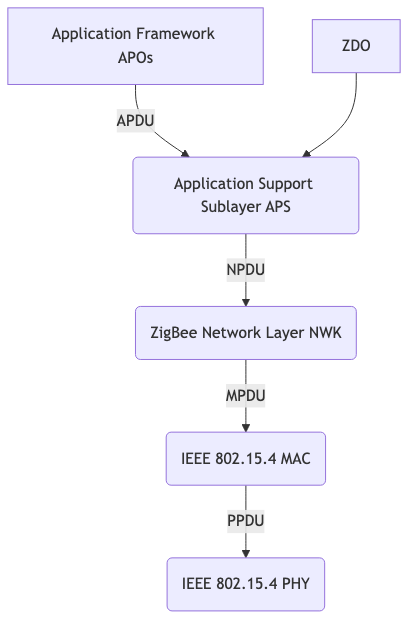
\includegraphics[keepaspectratio,alt={Stack protocollare di ZigBee e incapsulamento da Application ad IEEE 802.15.4.}]{images/mermaid-03-livello-mac-e-reti-wsn-01.png}}
\caption{Stack protocollare di ZigBee e incapsulamento da Application ad
IEEE 802.15.4.}
\end{figure}

\pandocbounded{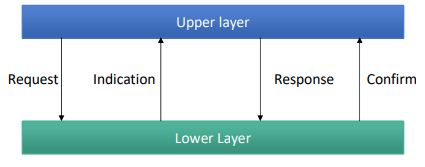
\includegraphics[keepaspectratio]{images/Pasted-image-20260309111946.png}}

\subsection{Formazione della Rete e Indirizzamento ad
Albero}\label{formazione-della-rete-e-indirizzamento-ad-albero}

La rete ha tre ruoli logici: \textbf{Network Coordinator} (FFD, crea la
rete), \textbf{Router} (FFD, instrada traffico), \textbf{End-Device}
(RFD/FFD). La creazione della PAN (\emph{Network Formation}) è eseguita
dal Coordinator con un energy/active scan per trovare canali liberi.
Sceglie un PAN ID, si autoassegna l'indirizzo \(0\times0000\) e avvia i
beacon.

L'\textbf{ingresso} in rete avviene tramite \emph{Join through
Association} (device avvia scansione e si associa al padre) oppure
\emph{Direct Join} (un nodo forza l'aggregazione al figlio conosciuto).

\textbf{Allocazione degli Indirizzi (Tree Structure)}: ZigBee
pre-distribuisce blocchi di indirizzi per assegnazioni veloci e
scalabili, evitando collisioni. I parametri hardware del coordinator
sono fissi: \(R_m\) (max router figli), \(D_m\) (max end-device figli),
\(L_m\) (profondità massima albero). La grandezza del blocco per un
router a profondità \(d\) è \(C_{skip}(d)\): \[
C_{skip}(d) = \begin{cases} 1 & \text{se } d = L_m \\ 1 + R_m \cdot C_{skip}(d+1) + D_m & \text{altrimenti} \end{cases}
\] I figli router riceveranno gli indirizzi saltando segmenti pari a
\(C_{skip}(d+1)\).

\subsection{Routing}\label{routing}

ZigBee supporta instradamento differenziato, e le logiche possono
coesistere: - \textbf{Tree Routing}: segue i rami logici dell'albero
formati in fase di join. È compatibile col beaconing ma può usare
cammini non ottimali. - \textbf{Mesh Routing}: ispirato ad AODV. Usa la
\textbf{Routing Table} per inoltri diretti. In caso di rotta mancante,
usa il \emph{Route Discovery Protocol} diffondendo in broadcast messaggi
\texttt{RREQ} per trovare la destinazione. Il \texttt{RREP} torna
indietro memorizzando il ``Residual Cost'' nelle routing table. Molto
flessibile e robusto, ma non permette una rete globalmente sincronizzata
a superframe.

\begin{center}\rule{0.5\linewidth}{0.5pt}\end{center}

\section{4. Application Layer: ZDO, APS e ZCL (Lezione
12)}\label{application-layer-zdo-aps-e-zcl-lezione-12}

\pandocbounded{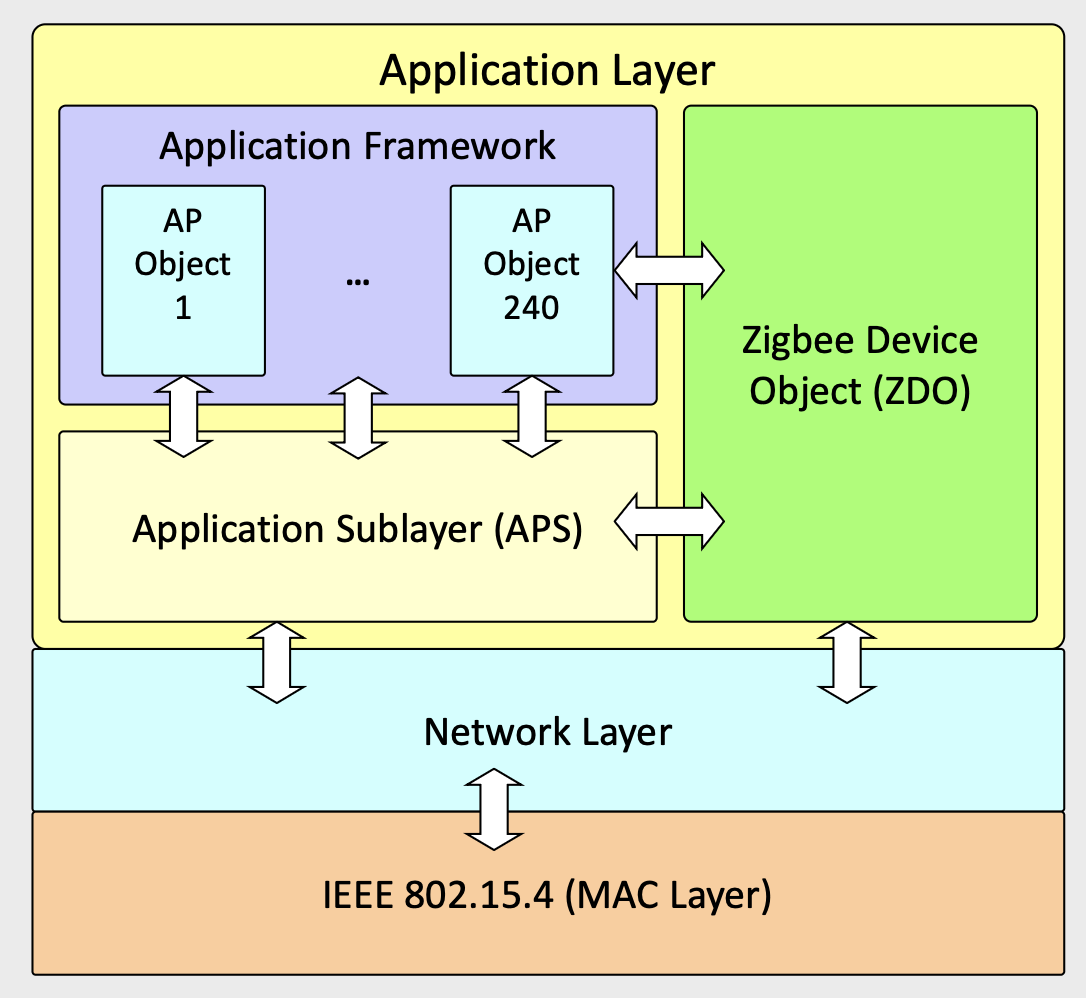
\includegraphics[keepaspectratio]{images/Pasted-image-20260317144430.png}}

Il livello Applicativo poggia su tre pilastri: 1. \textbf{Application
Framework ed Endpoints}: Fino a 240 applicazioni coesistenti (APO) su un
singolo device. Ogni applicazione risiede in un endpoint numerato da 1 a
240. L'Endpoint 0 è sempre fisso e riservato al componente ZDO. 2.
\textbf{ZigBee Device Object (ZDO)}: È il manager che controlla
localmente la logica della rete: offre i servizi di \emph{Device e
Service Discovery} all'utente, gestisce le direttive di \emph{Binding} e
assicura il \emph{Node Management} secondo il proprio ruolo hardware. 3.
\textbf{Application Support Sublayer (APS)}: È il ``Transport layer'' di
ZigBee. Filtra indirizzi, assicura la ricezione tramite conferme
applicative end-to-end, e memorizza le tabelle multicast (Group
Management).

\subsection{La ZigBee Cluster Library (ZCL) e i
Profili}\label{la-zigbee-cluster-library-zcl-e-i-profili}

Un \textbf{Cluster} è l'unità base funzionale: definisce formalmente i
\textbf{Comandi} attuabili e gli \textbf{Attributi} di stato esposti. È
identificato da 16-bit (es. OnOff Cluster \(0\times0006\)). Un
\textbf{Application Profile} raggruppa comportamenti per
interoperabilità (es. Home Automation \texttt{0104}). \emph{Device IDs}
identificano visivamente il dispositivo (una lampadina o termostato) ma
NON servono per il Service Discovery.

La \textbf{ZCL} è un archivio enorme di cluster pre-confezionati dalla
ZigBee Alliance per evitare che le industrie reinventino la logica
applicativa. Supporta un'architettura \textbf{Client/Server} in cui il
\emph{Dynamic Attribute Reporting} spinge in automatico le variazioni al
client risparmiando l'energia di un continuo polling in lettura.

\subsection{APS Binding e Indirizzamento
Indiretto}\label{aps-binding-e-indirizzamento-indiretto}

Il \textbf{Binding} (servito dal livello APS) crea una connessione
virtuale persistente tra un cluster su un nodo e uno remoto, pur non
conoscendone le coordinate logiche a priori. Dispositivi basici si
limitano a inviare dati verso un endpoint generico. L'APS layer sfrutta
la \textbf{Binding Table} combinata con l'\textbf{Address Map Table}
(che fissa la traduzione tra indirizzo fisico MAC e quello volatile NWK
16-bit) per instradare a livello software il pacchetto. Anche in caso di
riavvio logico della rete, il ponte applicativo non si spezza mai.

\pandocbounded{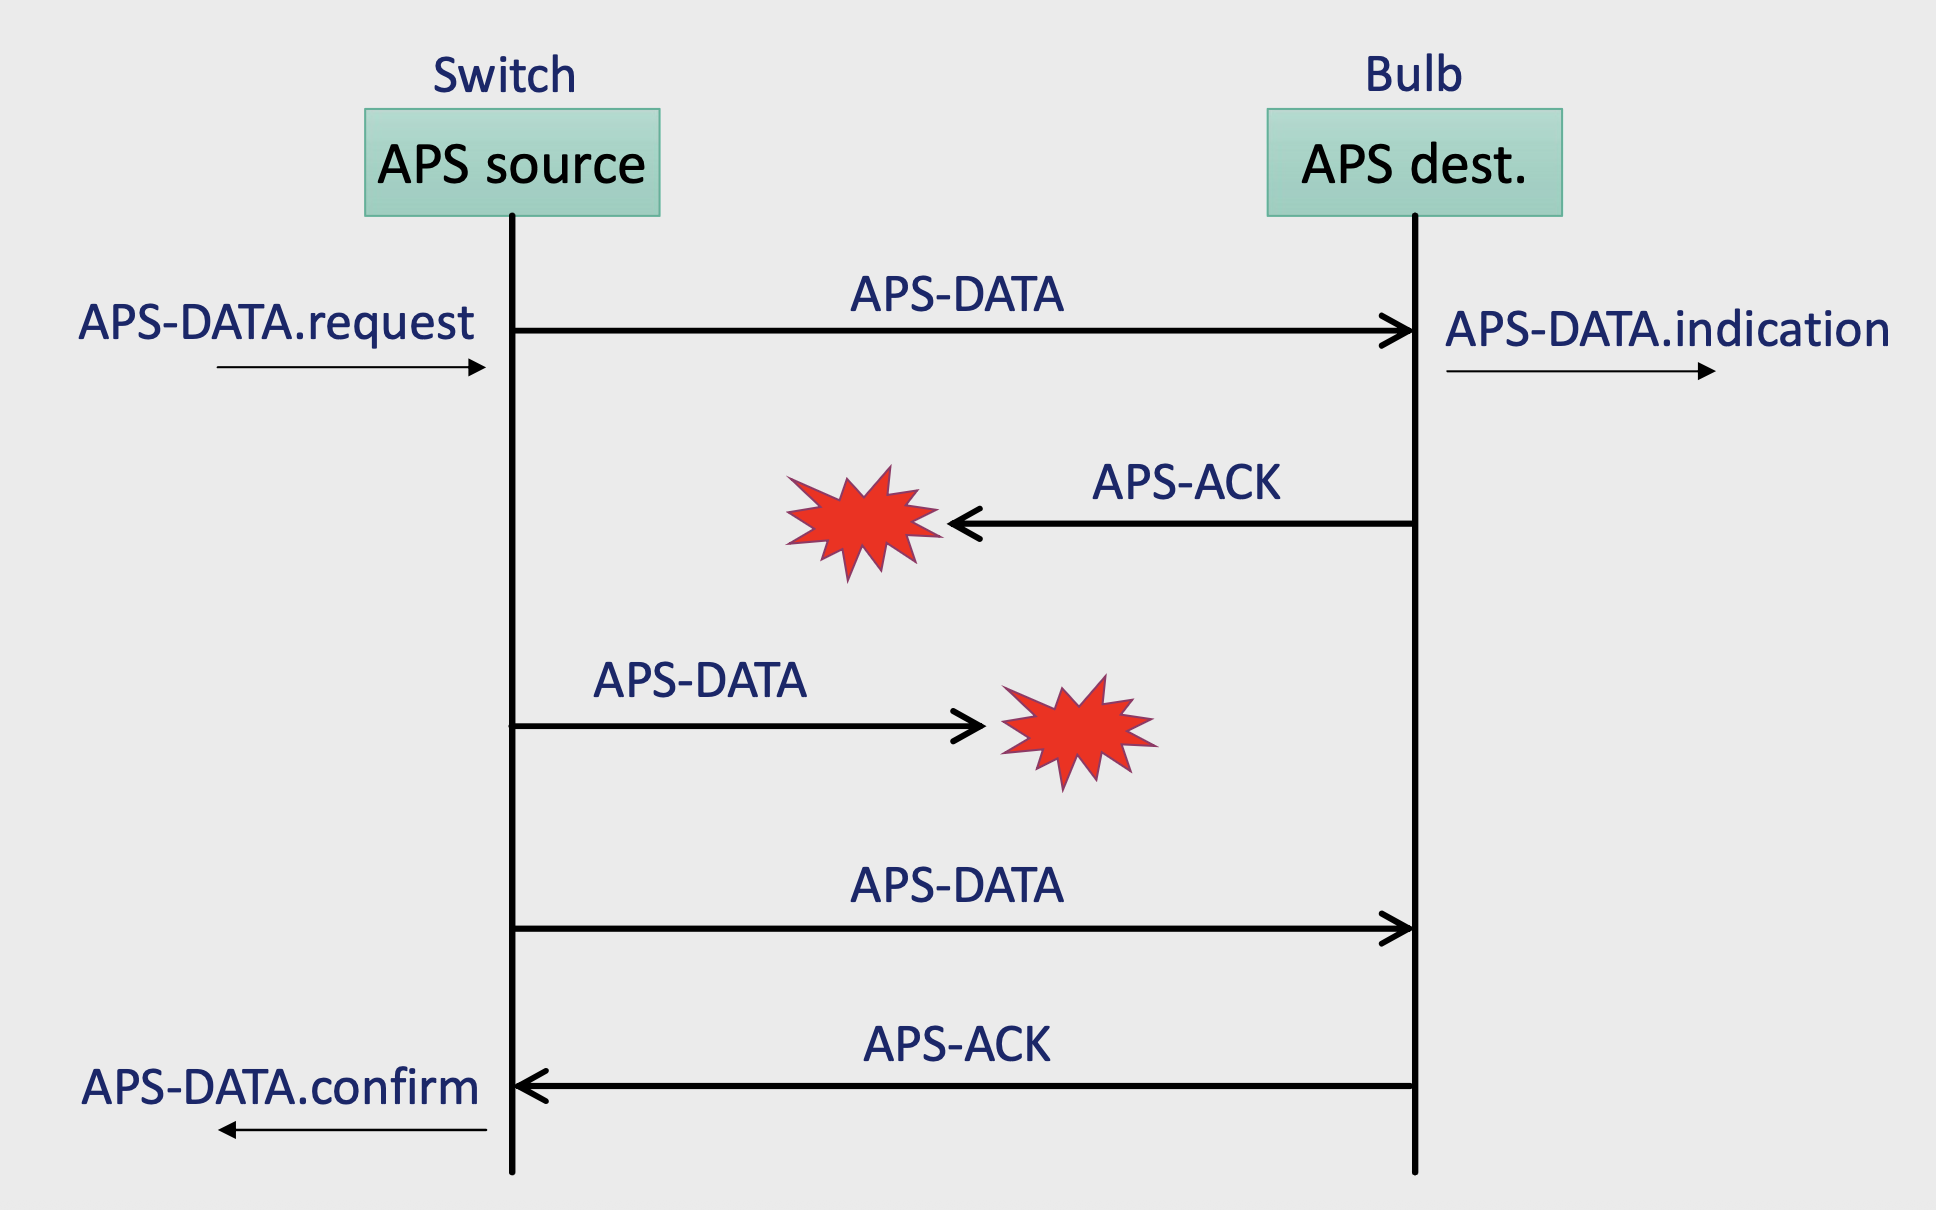
\includegraphics[keepaspectratio]{images/Pasted-image-20260317150017.png}}

\textbf{Esempio Applicativo (Indoor Localization)}: Tramite l'analisi
dell'RSSI radio è supportato il \emph{Remote Positioning} (le ancore
recepiscono e computano i segnali mobili) o il \emph{Self Positioning}
(il mobile triangola i fari delle ancore). In ZigBee, tramite
l'\emph{RSSI Location Cluster}, paradossalmente il nodo mobile si
atteggia a ``Server'' del Cluster, in quanto sorgente dei dati logici, e
il nodo ancorato legge come ``Client''.

\begin{center}\rule{0.5\linewidth}{0.5pt}\end{center}

\section{5. ZigBee Security (Lezione
13)}\label{zigbee-security-lezione-13}

ZigBee definisce un framework imperativo basato su: \emph{key
establishment}, \emph{key transport}, \emph{frame protection} e
\emph{device management}. La logica fondamentale prevede che \textbf{il
livello che origina il messaggio debba essere colui che provvede alla
messa in sicurezza}. Quasi tutto il traffico subisce cifratura a livello
NWK per proteggere dal ``theft of service'' (tranne i fisiologici
messaggi aperti per l'associazione iniziale). Il framework impone severe
routine di gestione per le perdite di sincronizzazione crittografiche o
overflow.

\subsection{Architettura di Sicurezza}\label{architettura-di-sicurezza}

\begin{itemize}
\tightlist
\item
  \textbf{NWK Layer}: Si assicura che ogni hop sia cifrato e integro e
  inserisce contatori anti-replay (\emph{Freshness}).
\item
  \textbf{APS Layer}: Eroga i servizi crittografici veri e propri, cifra
  carichi di lavoro end-to-end e trasporta in via logica le chiavi.
\item
  \textbf{ZDO}: Il manager strategico che dirige le policy e ordina
  all'APS le manovre da fare.
\end{itemize}

\textbf{Chiavi a 128-bit}: 1. \textbf{Network key}: Usata su base
collettiva. 2. \textbf{Link keys}: Sessioni dirette tra un nodo A e un
nodo B (per comunicazioni esclusive). 3. \textbf{Master key}: Non è
usata per cifrare traffico dati vivo, ma viene sfruttata da algoritmi
hash unidirezionali per generare in autonomia nuove Link Keys.

\subsection{Symmetric-Key Key Establishment (SKKE) e Trust
Center}\label{symmetric-key-key-establishment-skke-e-trust-center}

SKKE è il processo gestito dal livello APS che permette a due nodi di
ricavare una nuova Link Key per derivazione tramite una sequenza
\emph{challenge-response} di scambio di numeri effimeri aleatori e hash
applicati a un pre-segreto (Trust Provisioning). I nodi derivano la
chiave, poi confermano per scrupolo di aver ottenuto lo stesso match.

In ogni rete blindata c'è e deve esserci \textbf{un solo Trust Center}
designato, autorizzato a validare l'ingresso nella rete e ad erogare
centralmente il materiale crittografico ai nodi al momento del
\emph{join} (sfruttando chiavi Master per aprire prima tunnel provvisori
se necessario). Nelle reti domestiche, le funzioni del Trust Center sono
semplicemente incluse e assorbite dal Coordinator.

\begin{center}\rule{0.5\linewidth}{0.5pt}\end{center}

\begin{calloutnote}{Domande d’esame e Concetti Chiave di Riepilogo}

- Compromesso MAC: energia vs.~latenza e throughput. Differenza tra Sync
(S-MAC), Preamble Sampling (B-MAC, X-MAC, BoX-MAC) e Polling. - B-MAC:
necessità di un preambolo più lungo della finestra di sleep. X-MAC
riduce il tempo interrompendolo al read dell'ID; BoX-MAC ripete in
catena il pacchetto stesso. - IEEE 802.15.4: Bande libere (es. 2.4 GHz
globale). Ruoli (FFD, RFD). Formato superframe: l'indispensabilità del
CAP a prescindere dal CFP/GTS. Protocollo di Associazione MAC. -
Architettura ZigBee: I tre livelli superiori (NWK, ZDO, APS, Application
Framework). \(C_{skip}(d)\) nell'indirizzamento ad albero statico. Mesh
Routing (RREQ/RREP stile AODV) contro Tree Routing (supporta beaconing
ma rotta fissa). - ZDO (Endpoint 0), ZCL e Profiling. Il binding
indiretto tramite APS. Il concetto di Client/Server nel Reporting
dinamico. - Sicurezza NWK e Trust Center univoco in rete per
distribuzione e validazione delle chiavi crittografiche (Network, Link e
Master Key). SKKE challenge-response.

\end{calloutnote}

\newpage

\chapter{Gestione Energetica: Energy Harvesting e
Neutralità}\label{gestione-energetica-energy-harvesting-e-neutralituxe0}

Il problema di fondo dei dispositivi IoT è energetico: alimentarli con
una batteria di capacità finita costringe a scegliere tra prestazioni e
durata. Una batteria grande permette lunga vita, ma aumenta dimensioni,
peso e costo; un processore a basso consumo estende la vita ma limita
potenza di calcolo e portata radio. L'\textbf{energy harvesting}
(raccolta di energia) rappresenta un'alternativa strutturale: invece di
ottimizzare il consumo, si raccoglie energia dall'ambiente e si elimina
--- o si riduce drasticamente --- il vincolo della batteria finita.

Se la sorgente è abbondante e disponibile in modo continuo o periodico,
il dispositivo può funzionare «per sempre». Questa prospettiva sposta
l'obiettivo del progettista dalla massimizzazione della vita utile alla
massimizzazione delle prestazioni a parità di disponibilità energetica.

\begin{center}\rule{0.5\linewidth}{0.5pt}\end{center}

\section{Definizioni fondamentali}\label{definizioni-fondamentali}

Tre concetti strutturano l'intero dominio:

\begin{itemize}
\tightlist
\item
  \textbf{Energy source} (sorgente di energia): la fonte primaria (sole,
  vento, vibrazioni, ecc.) da cui l'energia viene estratta.
\item
  \textbf{Harvesting source} (tecnologia di raccolta): il componente
  fisico --- cella solare, turbina, cristallo piezoelettrico, antenna
  --- che converte la sorgente in energia elettrica. La produzione varia
  nel tempo e in funzione delle condizioni ambientali, ed è generalmente
  al di fuori del controllo del progettista.
\item
  \textbf{Load} (carico): l'energia consumata dal dispositivo per le
  proprie attività. Un dispositivo IoT ha molteplici sottosistemi
  (processore, radio, storage, trasduttori/ADC), ciascuno con stati
  propri e consumi differenti; il carico varia quindi nel tempo a
  seconda delle attività in esecuzione.
\end{itemize}

\begin{calloutdefinition}{Harvesting System}

Un sistema che supporta un carico variabile alimentato da una sorgente
di harvesting variabile, anche quando la potenza istantanea della
sorgente non corrisponde al carico.

\end{calloutdefinition}

Il problema chiave è il \textbf{disaccoppiamento} tra produzione e
consumo: la sorgente produce quando l'ambiente lo consente, il
dispositivo consuma quando deve eseguire i propri task.

Esistono due approcci principali per adeguare produzione e consumo: 1.
\textbf{Adattare il carico} alla disponibilità energetica --- ad esempio
riducendo la frequenza di campionamento. 2. \textbf{Usare un buffer
energetico} --- una batteria ricaricabile o un supercapacitore che
accumula l'eccesso e lo cede nei momenti di deficit.

In pratica nessuno dei due approcci è sufficiente da solo: il carico non
può essere ridotto arbitrariamente senza compromettere la funzionalità,
e il buffer è fisicamente limitato e non ideale (ha perdite ed
efficienza di carica \(< 1\)).

\begin{center}\rule{0.5\linewidth}{0.5pt}\end{center}

\section{Architetture di harvesting}\label{architetture-di-harvesting}

\subsection{Harvest-Use}\label{harvest-use}

\begin{figure}
\centering
\pandocbounded{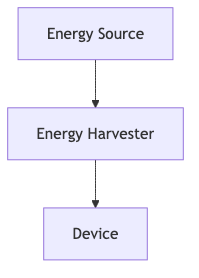
\includegraphics[keepaspectratio,alt={Schema logico dell'architettura Harvest-Use in cui l'energia raccolta alimenta direttamente il dispositivo}]{images/mermaid-04-gestione-energetica-01.png}}
\caption{Schema logico dell'architettura Harvest-Use in cui l'energia
raccolta alimenta direttamente il dispositivo}
\end{figure}

\emph{Fig. --- Architettura Harvest-Use: la sorgente alimenta
direttamente il dispositivo senza buffer.}

Nell'architettura \textbf{Harvest-Use} l'energia è raccolta esattamente
quando serve. Non esiste un buffer: la potenza prodotta \(P_s(t)\) viene
consumata istantaneamente. Il dispositivo è operativo solo se:

\[P_s(t) \geq P_c(t)\]

Questo comporta due forme di spreco: - Quando \(P_s(t) < P_c(t)\): il
dispositivo si spegne per mancanza di energia. - Quando
\(P_s(t) > P_c(t)\): l'eccesso \(P_s(t) - P_c(t)\) va perduto.

\subsection{Harvest-Store-Use}\label{harvest-store-use}

\begin{figure}
\centering
\pandocbounded{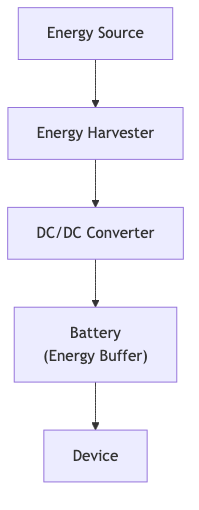
\includegraphics[keepaspectratio,alt={Schema dell'architettura Harvest-Store-Use che include un convertitore e un buffer di energia (batteria)}]{images/mermaid-04-gestione-energetica-02.png}}
\caption{Schema dell'architettura Harvest-Store-Use che include un
convertitore e un buffer di energia (batteria)}
\end{figure}

\emph{Fig. --- Architettura Harvest-Store-Use: l'energia in eccesso
viene accumulata nel buffer e prelevata nei momenti di deficit.}

Nell'architettura \textbf{Harvest-Store-Use} l'energia raccolta viene
immagazzinata nel buffer ogni volta che è disponibile e prelevata quando
la produzione è insufficiente o i task del dispositivo richiedono più
energia. Il buffer disaccoppia temporalmente produzione e consumo.

\subsubsection{Buffer ideale e non
ideale}\label{buffer-ideale-e-non-ideale}

Un buffer ideale ha capacità infinita, nessuna perdita ed efficienza di
carica \(\eta = 1\). Il dispositivo è sempre operativo se la carica
prodotta più quella iniziale eccede il consumo per ogni intervallo:
\[\int_0^T P_c(t)\,dt \leq \int_0^T P_s(t)\,dt + B_0 \qquad \forall T \in (0, \infty)\]

Un buffer reale ha capacità massima \(B_{\mathrm{max}}\), efficienza
\(\eta < 1\) e potenza di leakage \(P_{\mathrm{leak}}(t)\). La carica
\(B_T\) al tempo \(T\) deve soddisfare: \textbf{Conservazione
dell'energia (necessaria e sufficiente):}
\[B_T = B_0 + \eta\int_0^T [P_s - P_c]^+\,dt - \int_0^T [P_c - P_s]^+\,dt - \int_0^T P_{\mathrm{leak}}\,dt \geq 0\]

\textbf{Capacità finita (sufficiente, non necessaria):}
\[B_{\mathrm{max}} \geq B_0 + \eta\int_0^T [P_s - P_c]^+\,dt - \int_0^T [P_c - P_s]^+\,dt - \int_0^T P_{\mathrm{leak}}\,dt\]

\begin{callouttip}{Esercizio sul buffer non ideale}

Dispositivo con \(\eta = 95\%\), \(B_0 = 400\,\mathrm{mAh}\), leakage
trascurabile. Intervallo \([0, 4s]\): \(P_s = 80\,\mathrm{mA}\),
\(P_c = 150\,\mathrm{mA}\). Consumo supera produzione. Produzione =
\(0.089\,\mathrm{mAh}\), Consumo = \(0.167\,\mathrm{mAh}\).
\(B_4 = 400 + 0.089 - 0.167 = 399.922\,\mathrm{mAh}\) Intervallo
\([4s, 10s]\): \(P_s = 80\,\mathrm{mA}\), \(P_c = 20\,\mathrm{mA}\).
Produzione supera consumo. Produzione = \(0.133\,\mathrm{mAh}\), Consumo
= \(0.033\,\mathrm{mAh}\).
\(B_{10} = 399.922 + 0.95(0.133 - 0.033) = 400.017\,\mathrm{mAh}\)

\end{callouttip}

\begin{center}\rule{0.5\linewidth}{0.5pt}\end{center}

\section{Fonti di energia e
classificazione}\label{fonti-di-energia-e-classificazione}

Le sorgenti si classificano su due assi: \textbf{controllabilità} e
\textbf{prevedibilità}.

{\def\LTcaptype{none} % do not increment counter
\begin{longtable}[]{@{}
  >{\raggedright\arraybackslash}p{(\linewidth - 4\tabcolsep) * \real{0.3333}}
  >{\raggedright\arraybackslash}p{(\linewidth - 4\tabcolsep) * \real{0.3333}}
  >{\raggedright\arraybackslash}p{(\linewidth - 4\tabcolsep) * \real{0.3333}}@{}}
\toprule\noalign{}
\begin{minipage}[b]{\linewidth}\raggedright
Controllabilità
\end{minipage} & \begin{minipage}[b]{\linewidth}\raggedright
Descrizione
\end{minipage} & \begin{minipage}[b]{\linewidth}\raggedright
Esempi
\end{minipage} \\
\midrule\noalign{}
\endhead
\bottomrule\noalign{}
\endlastfoot
Completamente controllabile & L'energia è disponibile su richiesta &
Torcia shake-to-power, sorgenti RF dedicate \\
Parzialmente controllabile & Influenzabile ma non deterministica & Tag
RFID in ambiente RF non uniforme \\
Non controllabile & Raccolta solo quando disponibile & Sole, vento,
termica ambientale \\
\end{longtable}
}

Le sorgenti non controllabili si classificano in prevedibili (sole) e
non prevedibili (vibrazioni sismiche). La prevedibilità è fondamentale
per la pianificazione energetica.

\subsection{Dettaglio delle
Tecnologie}\label{dettaglio-delle-tecnologie}

\begin{itemize}
\tightlist
\item
  \textbf{RF harvesting}: I tag RFID passivi si alimentano
  esclusivamente con l'energia RF del reader.
\item
  \textbf{Piezoelettrico}: Converte deformazione meccanica in differenza
  di potenziale (es. solette per scarpe, pulsanti wireless).
\item
  \textbf{Energia solare ed Eolica}: Il sole produce in modo dipendente
  da latitudine, meteo e stagioni, con forte variabilità. La
  combinazione sole-vento (vento notturno, sole diurno) aumenta la
  copertura temporale, sebbene un harvesting non garantisca
  l'operatività continua per casi peggiori se mal dimensionati.
\end{itemize}

\begin{figure}
\centering
\pandocbounded{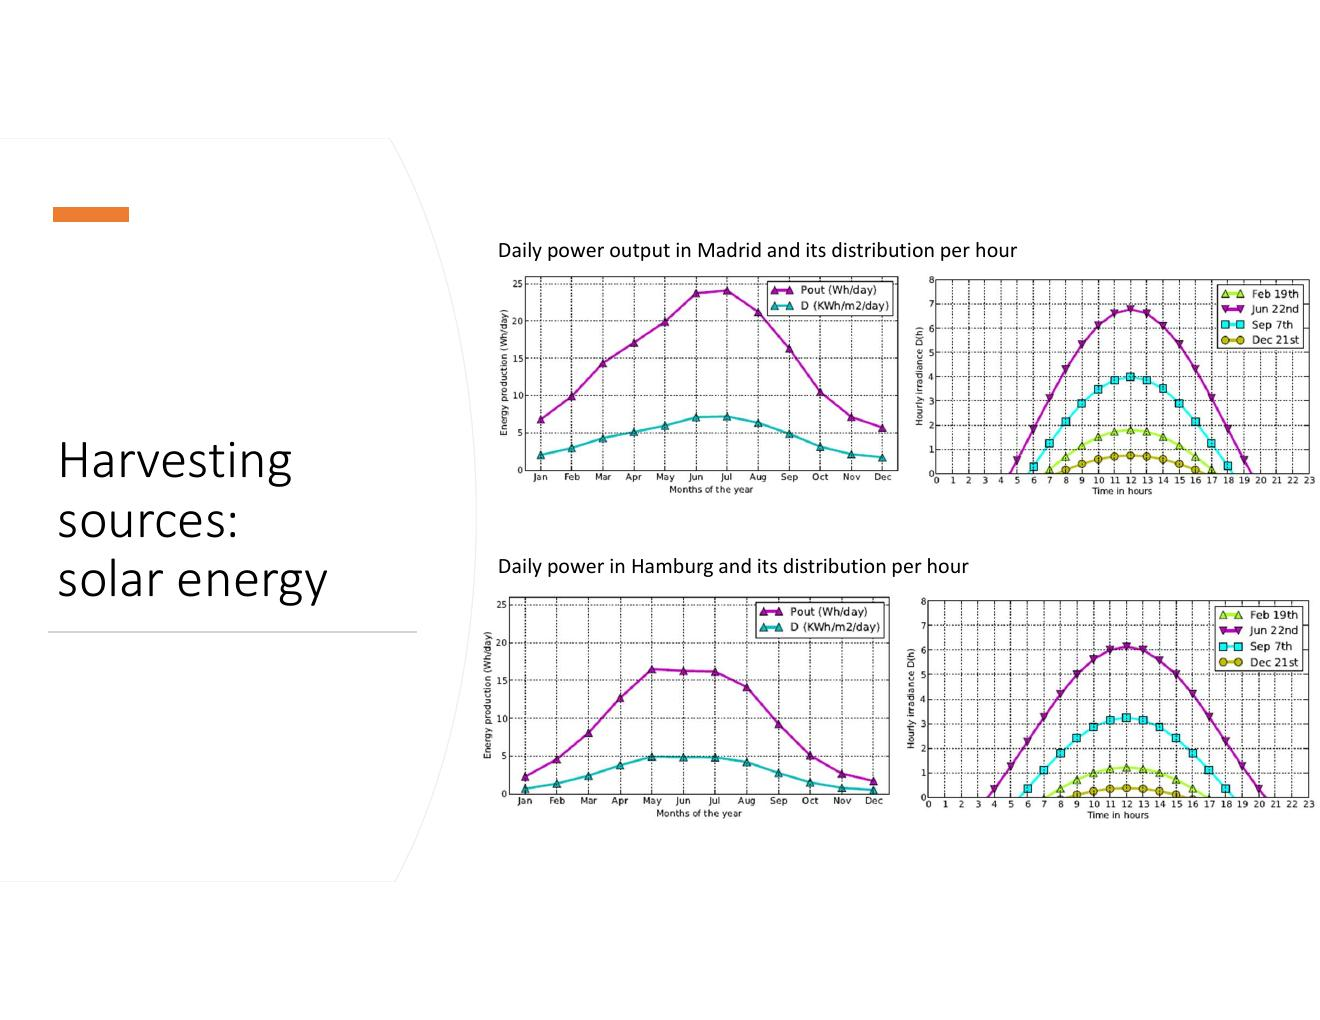
\includegraphics[keepaspectratio,alt={Produzione solare giornaliera a Madrid e Amburgo con distribuzione oraria}]{images/lezione-24-energy-harvesting-iot-img-01.jpg}}
\caption{Produzione solare giornaliera a Madrid e Amburgo con
distribuzione oraria}
\end{figure}

\begin{figure}
\centering
\pandocbounded{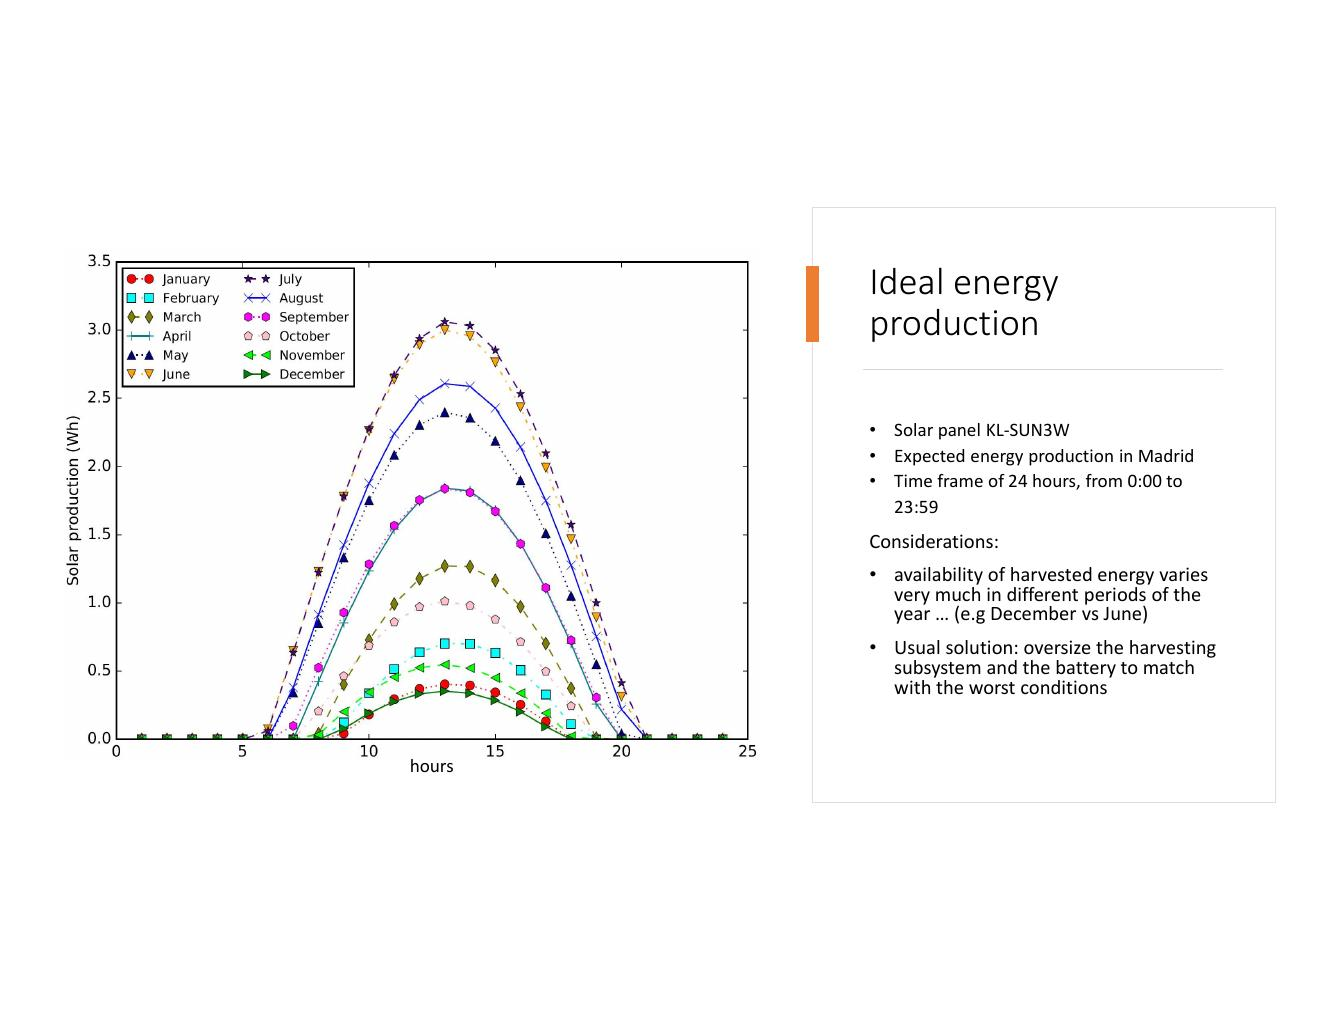
\includegraphics[keepaspectratio,alt={Produzione ideale mensile del pannello KL-SUN3W a Madrid}]{images/lezione-24-energy-harvesting-iot-img-02.jpg}}
\caption{Produzione ideale mensile del pannello KL-SUN3W a Madrid}
\end{figure}

\begin{figure}
\centering
\pandocbounded{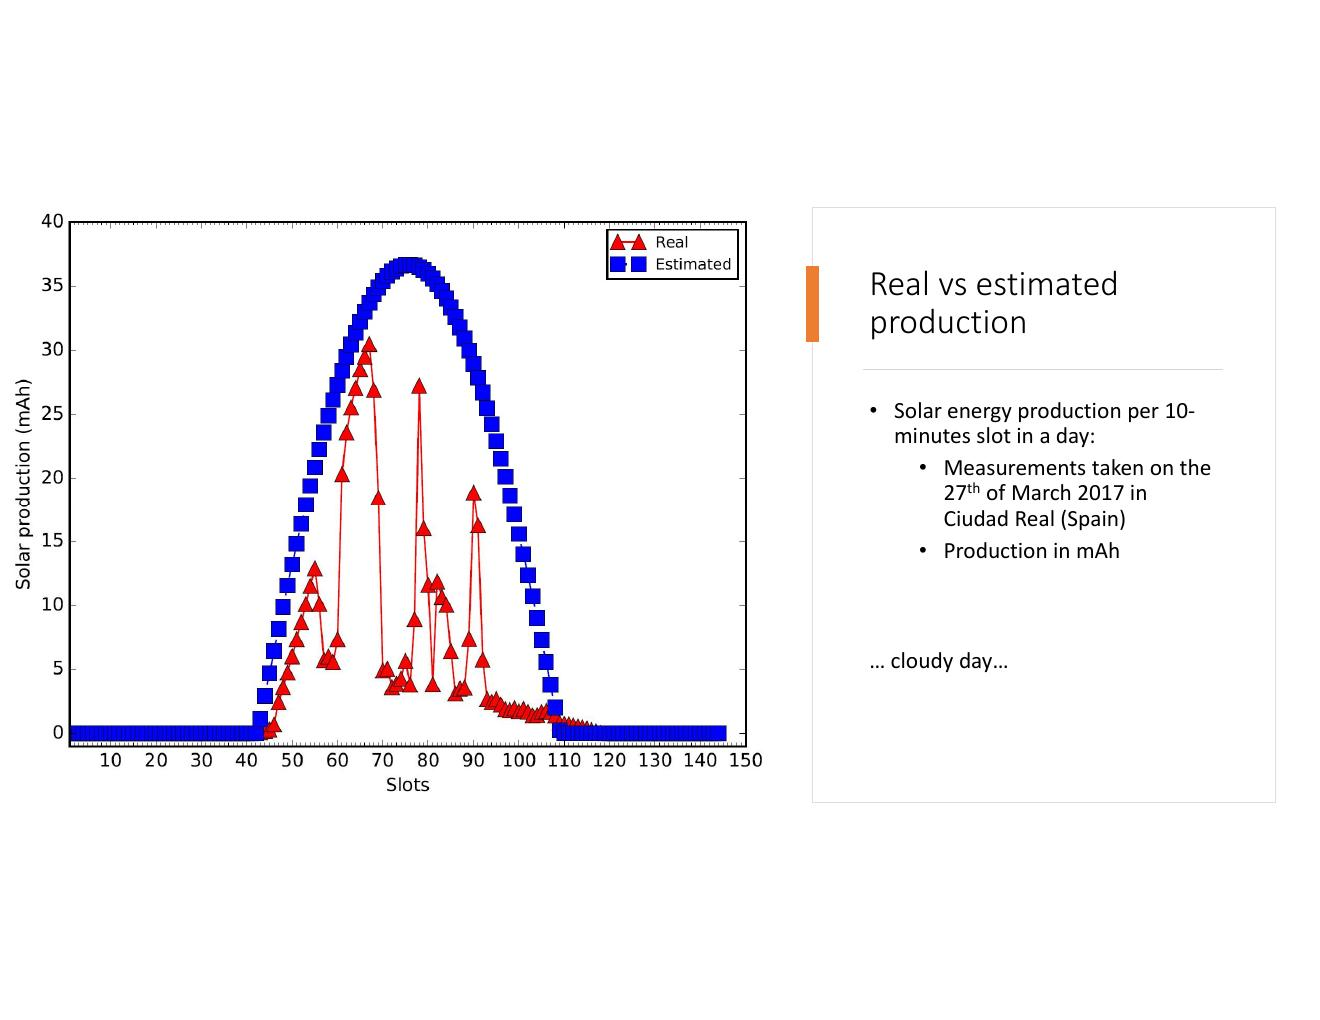
\includegraphics[keepaspectratio,alt={Produzione solare reale vs stimata --- Ciudad Real, 27 marzo 2017}]{images/lezione-24-energy-harvesting-iot-img-03.jpg}}
\caption{Produzione solare reale vs stimata --- Ciudad Real, 27 marzo
2017}
\end{figure}

\begin{figure}
\centering
\pandocbounded{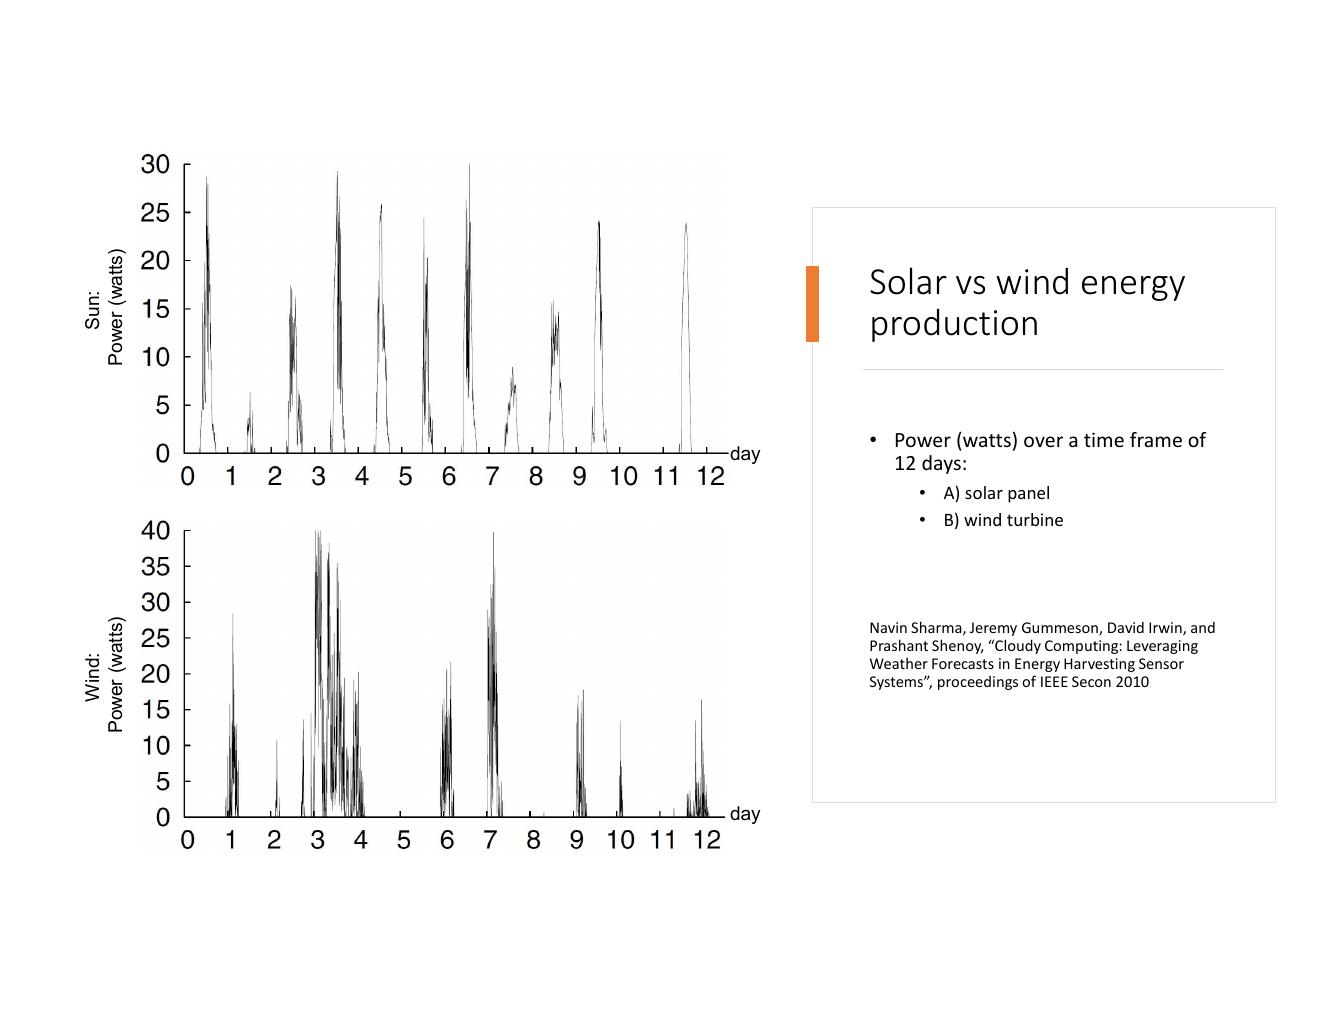
\includegraphics[keepaspectratio,alt={Confronto produzione solare vs eolica su 12 giorni}]{images/lezione-24-energy-harvesting-iot-img-04.jpg}}
\caption{Confronto produzione solare vs eolica su 12 giorni}
\end{figure}

\subsection{Tecnologie di storage}\label{tecnologie-di-storage}

\begin{itemize}
\tightlist
\item
  \textbf{Batterie Li-ion}: Preferite per l'IoT grazie a efficienza
  altissima (99.9\%), bassissimo self-discharge e alta densità.
\item
  \textbf{Supercapacitori}: Ricariche infinite, efficienza elevata.
  Ideali con energia disponibile a intervalli o forte jitter, tenuti
  carichi con trickle charge.
\end{itemize}

\begin{center}\rule{0.5\linewidth}{0.5pt}\end{center}

\section{Misurare la carica e la
produzione}\label{misurare-la-carica-e-la-produzione}

Tutte le tecniche di power management richiedono info fresche sulla
carica della batteria e la produzione.

La tensione a circuito aperto di una batteria decresce in modo circa
\textbf{lineare} nel range operativo.

\begin{figure}
\centering
\pandocbounded{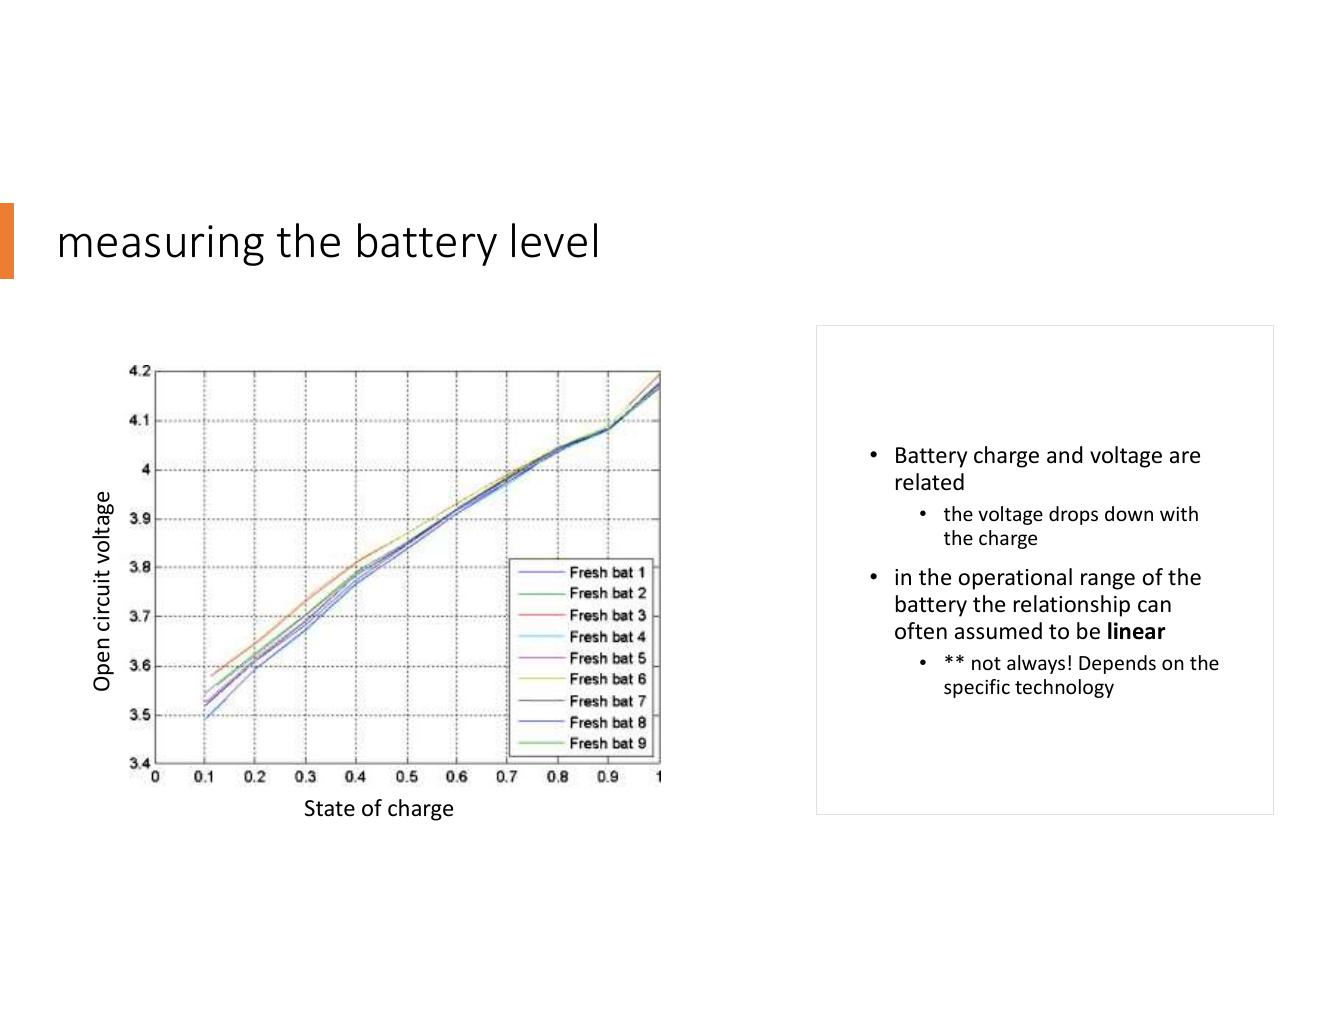
\includegraphics[keepaspectratio,alt={Tensione a circuito aperto vs stato di carica per batterie Li-ion}]{images/lezione-24-energy-harvesting-iot-img-05.jpg}}
\caption{Tensione a circuito aperto vs stato di carica per batterie
Li-ion}
\end{figure}

Tramite un ADC a \(d\) bit si legge la tensione per risalire alla
carica:
\[x_{\mathrm{max}} = 2^d - 1 \qquad x_{\mathrm{min}} = \mathrm{ROUND}\!\left(\frac{v_{\mathrm{min}}}{v_{\mathrm{ref}}}(2^d - 1)\right)\]
\[x = \mathrm{ROUND}\!\left(\frac{v}{v_{\mathrm{ref}}}(2^d - 1)\right)\]
\[B = B_{\mathrm{min}} + \frac{B_{\mathrm{max}} - B_{\mathrm{min}}}{x_{\mathrm{max}} - x_{\mathrm{min}}}(x - x_{\mathrm{min}})\]

\begin{callouttip}{Esercizio — Stima della carica da output ADC}

ADC a 10 bit, max carica 2000 mAh a 10V (batteria piena). A 8V residuo
200 mAh (min). Con \(d = 10\) bit si ha \(2^d - 1 = 1023\) e
\(v_{\mathrm{ref}} = 10\,\mathrm{V}\). \(x_{\mathrm{max}} = 1023\),
\(x_{\mathrm{min}} = 818\). Se ADC è 920:
\(B = 200 + \frac{920 - 818}{1023 - 818} \cdot 1800 \approx 1096\) mAh.
Se ADC è 830:
\(B = 200 + \frac{830 - 818}{1023 - 818} \cdot 1800 \approx 305\) mAh.
Se ADC è 1023: \(B = 2000\) mAh.

\end{callouttip}

\begin{center}\rule{0.5\linewidth}{0.5pt}\end{center}

\section{Neutralità energetica e Approccio di
Kansal}\label{neutralituxe0-energetica-e-approccio-di-kansal}

\begin{calloutdefinition}{Dispositivo energy-neutral}

Un dispositivo è \textbf{energy neutral} se riesce a mantenere il
livello di prestazione desiderato indefinitamente, senza mai esaurire la
batteria.

\end{calloutdefinition}

L'obiettivo è triplice: rimanere energy neutral, evitare lo spegnimento
e \textbf{massimizzare la utility}.

Kansal affronta il problema per sorgenti \textbf{non controllabili ma
prevedibili} (es. solare), modulando dinamicamente il duty cycle del
dispositivo tramite pianificazione slottata.

\subsection{Modello Formale: le Due
Condizioni}\label{modello-formale-le-due-condizioni}

\textbf{Condizione 1 --- Produzione di Energia:} L'energia totale
\(E_T = \int_T P_s(t) \, dt\) è bounded da un corridoio lineare:
\[\rho_s \cdot T - \sigma \leq E_T \leq \rho_s \cdot T + \sigma\] Dove
\(\rho_s\) è il trend medio e \(\sigma\) il burst bound.

\begin{figure}
\centering
\pandocbounded{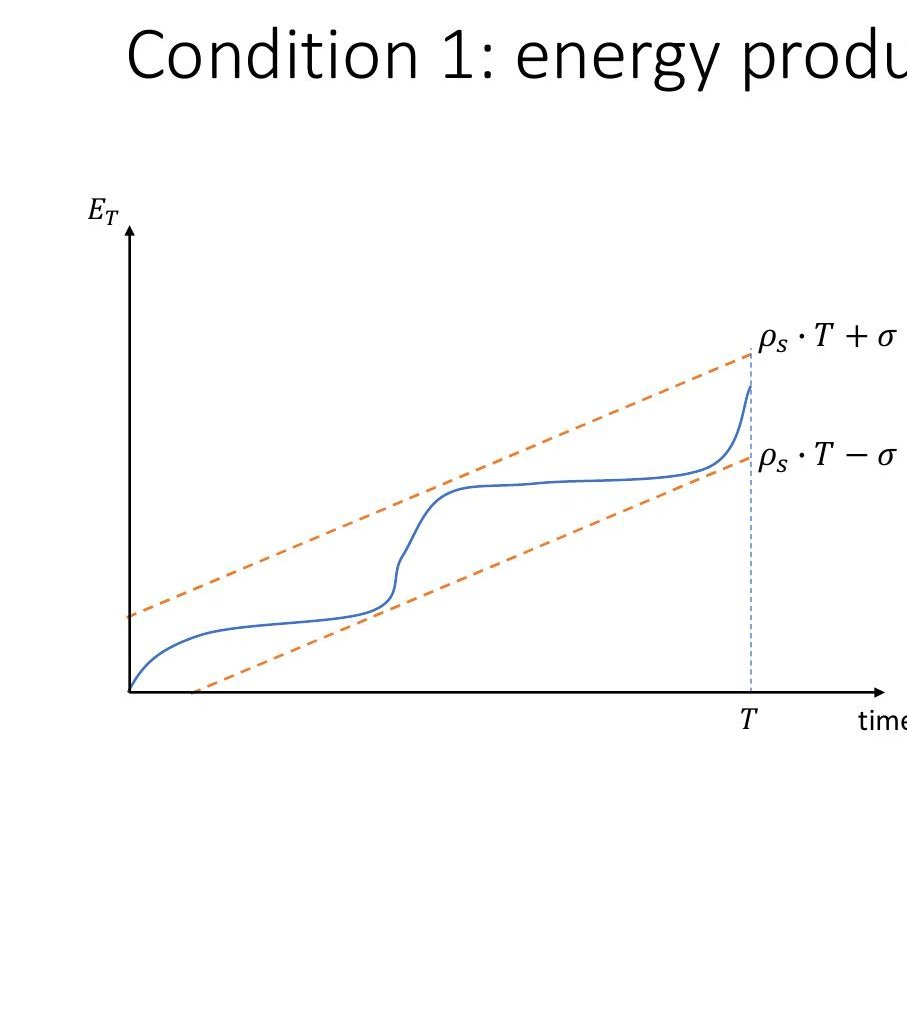
\includegraphics[keepaspectratio,alt={Grafico Condizione 1}]{images/lezione-28-kansal-problem-e-energy-neutrality-img-01.jpg}}
\caption{Grafico Condizione 1}
\end{figure}

\textbf{Condizione 2 --- Consumo (Load):} Il consumo
\(L_T = \int_T P_c(t) \, dt\) è bounded dall'alto:
\[0 \leq L_T \leq \rho_c \cdot T + \delta\]

\begin{figure}
\centering
\pandocbounded{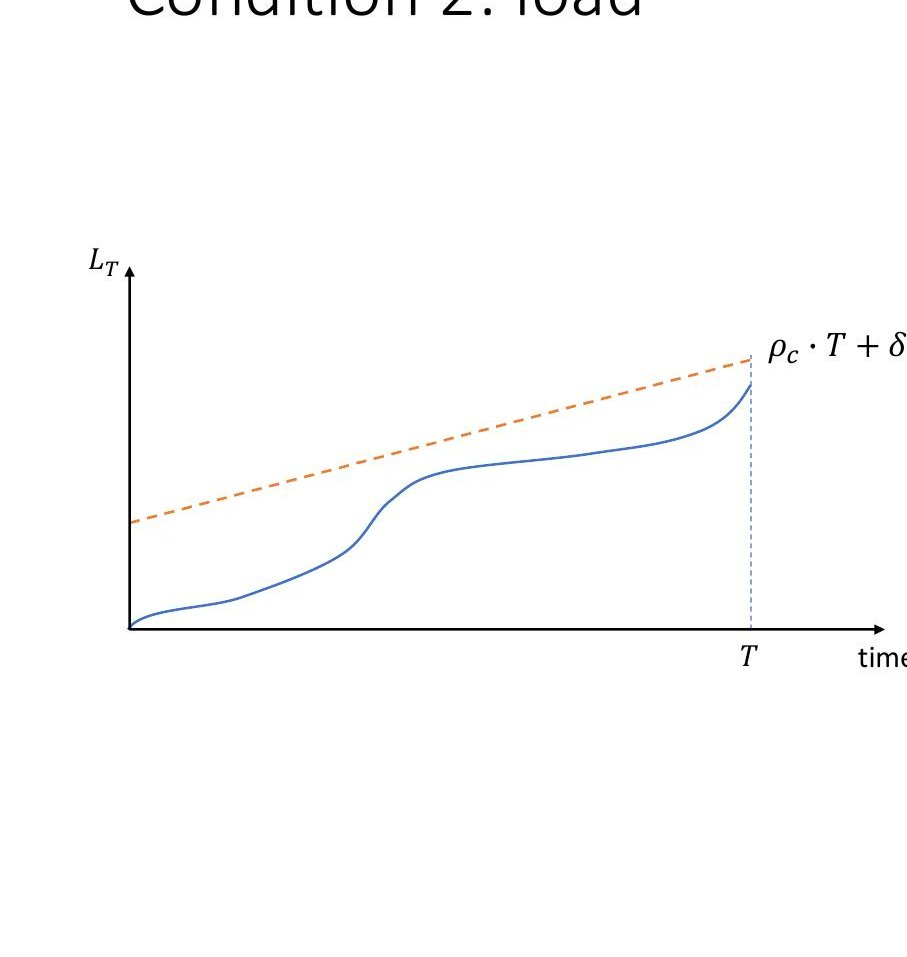
\includegraphics[keepaspectratio,alt={Grafico Condizione 2}]{images/lezione-28-kansal-problem-e-energy-neutrality-img-02.jpg}}
\caption{Grafico Condizione 2}
\end{figure}

\begin{callouttheorem}{Teorema di Kansal (Condizione sufficiente)}

Se le due condizioni valgono, con efficienza di carica \(\eta\) e
leakage \(\rho_{leak}\), il sistema è energy neutral se: 1.
\(\eta \rho_s \geq \rho_c + \rho_{leak}\) (trend di produzione copre
consumo e perdita) 2. \(B_0 \geq \eta\sigma + \delta\) (carica iniziale
sufficiente ai burst) 3. \(B_{max} \geq B_0\) (ammissibilità fisica)

\end{callouttheorem}

\subsection{Utility e Duty Cycle}\label{utility-e-duty-cycle}

Il sistema modula il \textbf{duty cycle (dc)} per limitare il consumo e
massimizzare una funzione \textbf{utility \(u(dc)\)}:

\[u(dc) = \begin{cases} 0 & \text{se } dc < dc_{min} \\ \alpha \cdot dc + \beta & \text{se } dc_{min} \leq dc \leq dc_{max} \\ u_M & \text{se } dc > dc_{max} \end{cases}\]

\begin{figure}
\centering
\pandocbounded{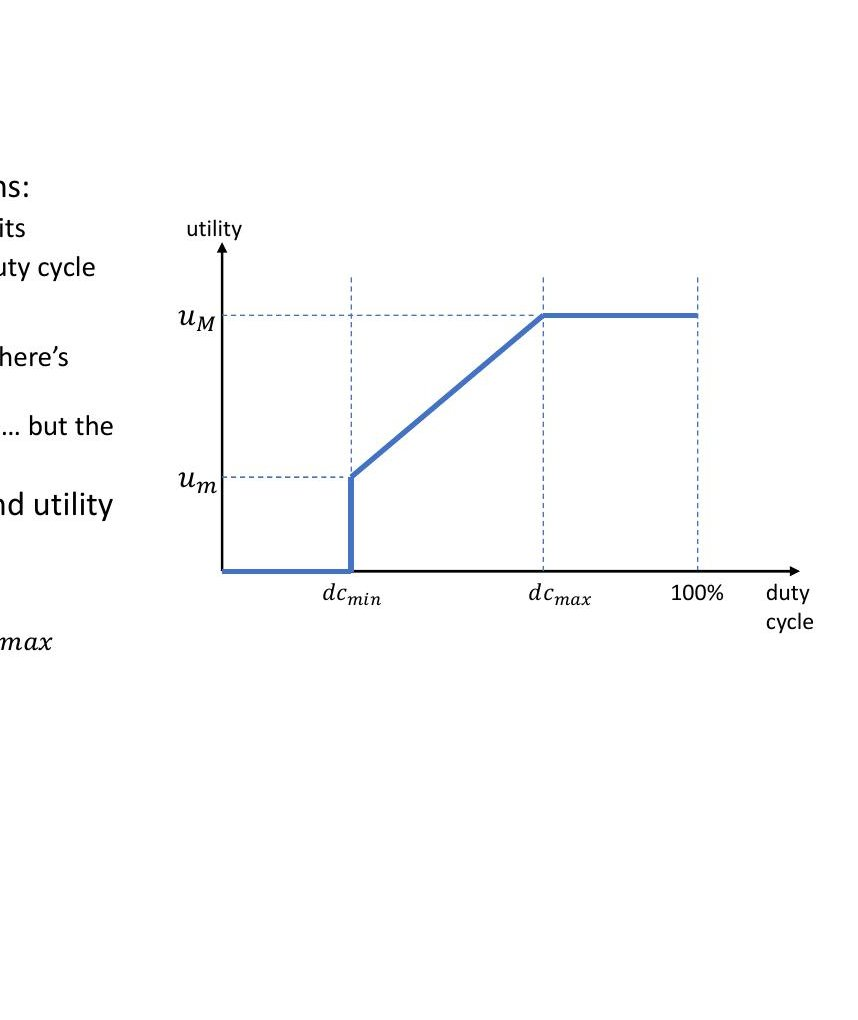
\includegraphics[keepaspectratio,alt={Funzione utility vs duty cycle}]{images/lezione-28-kansal-problem-e-energy-neutrality-img-03.jpg}}
\caption{Funzione utility vs duty cycle}
\end{figure}

Il consumo di potenza si modella come lineare
\(p(dc) = \rho \cdot dc + \sigma\).

\subsection{Previsione: EWMA}\label{previsione-ewma}

Si utilizza il filtro \textbf{EWMA} per stimare la produzione slot per
slot:
\[\tilde{p}_{j+1}(i) = \alpha \cdot p_j(i) + (1 - \alpha) \cdot \tilde{p}_j(i)\]
La produzione di oggi aiuta a stimare quella di domani. L'errore è più
alto attorno a mezzogiorno, ma in generale la produzione solare è
ripetibile giorno per giorno.

\begin{figure}
\centering
\pandocbounded{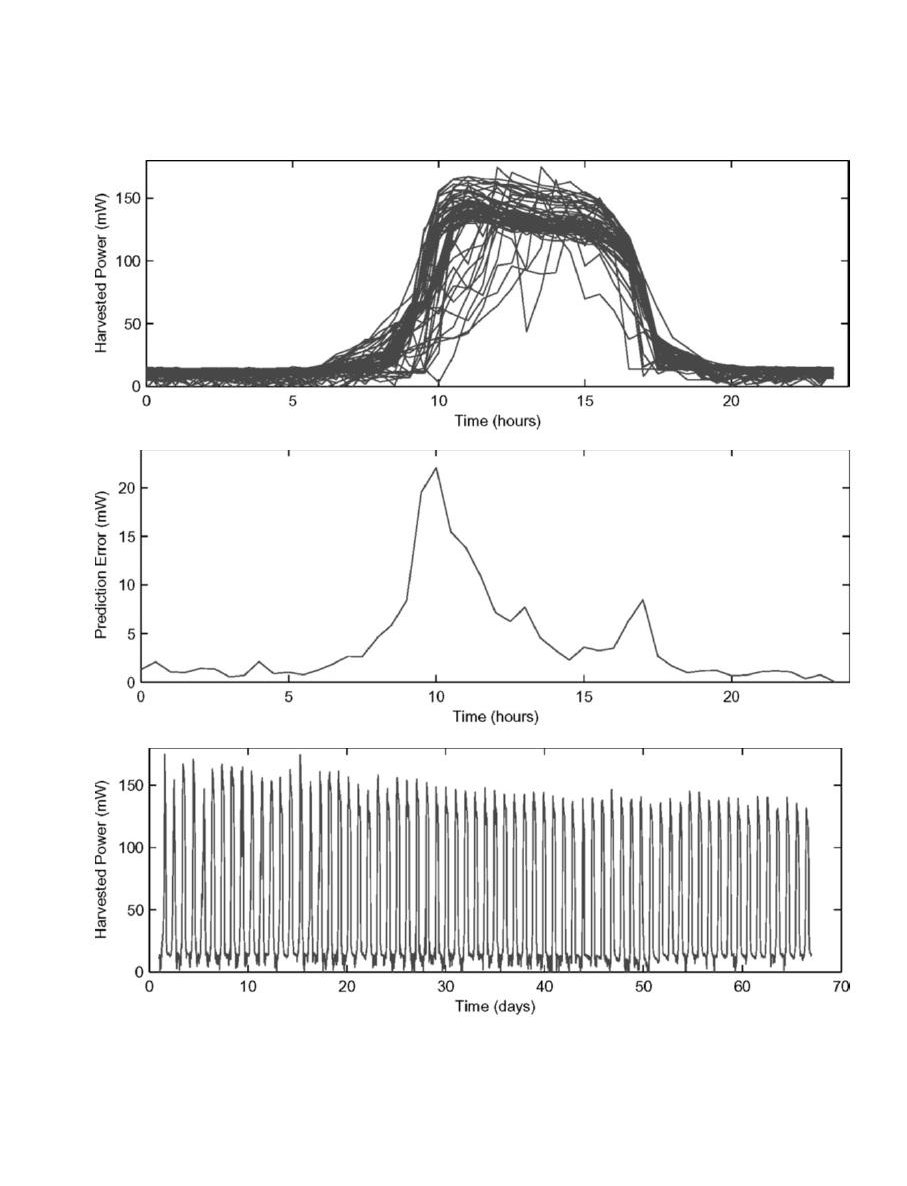
\includegraphics[keepaspectratio,alt={Esperimenti con Heliomote e EWMA}]{images/lezione-28-kansal-problem-e-energy-neutrality-img-04.jpg}}
\caption{Esperimenti con Heliomote e EWMA}
\end{figure}

\subsection{L'Algoritmo di Kansal}\label{lalgoritmo-di-kansal}

Assegnazione iniziale: per gli slot ``di sole'' (\(S\), in cui
produzione \(\ge p_{max}\)) il dc è \(dc_{max}\). Negli slot ``bui''
(\(D\), produzione \(< p_{max}\)) il dc è \(dc_{min}\). Poi si calcola
il \textbf{surplus residuo} \(p_{res} = B(k+1) - B(1)\).

\begin{enumerate}
\def\labelenumi{\arabic{enumi}.}
\tightlist
\item
  \textbf{Caso 1 --- Sovraproduzione (\(p_{res} > 0\)):} Usa l'energia
  avanzata per alzare al massimo il dc dei dark slot, uno per volta. Il
  residuo finale alza parzialmente l'ultimo dark slot toccato.
\item
  \textbf{Caso 2 --- Sottoproduzione (\(p_{res} < 0\)):} Manca energia.
  Controlla che una riduzione uniforme sui sun slot (\(|p_{res}|/|S|\))
  basti (entro \(p_{max} - p_{min}\)). Se sì, abbassa uniformemente il
  duty cycle in tutti i sun slot.
\end{enumerate}

\begin{callouttip}{Propriet�}

È ottimale, semplice, leggero. Se la produzione reale differisce, lo
scheduler riadatta la pianificazione dinamicamente per i restanti slot.
Limite: si modella solo il dc, ma non scelte tra trasduttori,
protocolli, algoritmi.

\end{callouttip}

\subsubsection{Esercizio Risolto 1
(Surplus)}\label{esercizio-risolto-1-surplus}

Dati: \(dc_{max}=90\%, p_{max}=5, u=100\);
\(dc_{min}=50\%, p_{min}=1, u=10\). Formule: \(p(dc)=0.1\cdot dc - 4\),
\(u(dc)=2.25\cdot dc - 102.5\). Slot
\(\tilde{p}_s = [0, 0, 0, 2, 6, 11, 10, 7, 3, 0, 0, 0]\). Slot di sole
(\(S\)): 5, 6, 7, 8 (qui partono a \(p_{max}=5\)). Gli altri partono a
\(p_{min}=1\). Prodotto = 39. Consumato =
\(8 \times 1 + 4 \times 5 = 28\). \(p_{res} = 11 > 0\).
\(p_{diff} = 4\). Con 11 surplus, posso portare \(11//4 = 2\) dark slot
(1 e 2) al massimo. Restano 3 di surplus, usati per lo slot 3,
portandolo a un consumo di \(1+3=4\). Per lo slot 3, il
\(dc = (4+4)/0.1 = 80\%\), \(u = 77.5\).

\subsubsection{Esercizio Risolto 2
(Deficit)}\label{esercizio-risolto-2-deficit}

Stessi dati base, ma \(p_{min}=2\). Nuove formule:
\(\rho=0.075, \sigma=-1.75\). Slot
\(\tilde{p}_s = [0, 0, 1, 3, 5, 8, 4, 3, 2, 0, 0, 0]\). Slot di sole: 5,
6. Gli altri a \(p_{min}=2\). Prodotto = 26. Consumato =
\(10 \times 2 + 2 \times 5 = 30\). \(p_{res} = -4 < 0\). Controllo
ammissibilità: \((5-2) > 4/2 \rightarrow 3 > 2\). Ammissibile. Abbasso
consumo dei sun slot di \(|p_{res}|/|S| = 4/2 = 2\). Consumo dei sun
slot diventa \(5-2=3\). \(dc\) dei sun slot:
\(dc = (3+1.75)/0.075 = 63.3\%\). L'utility è \(42.4\).

\begin{center}\rule{0.5\linewidth}{0.5pt}\end{center}

\section{Modello Task-Based per la Neutralità
Energetica}\label{modello-task-based-per-la-neutralituxe0-energetica}

Kansal non modella la complessità di vere applicazioni IoT che hanno
diverse fasi (Sensing \(\rightarrow\) Storing \(\rightarrow\) Processing
\(\rightarrow\) Transmitting) ciascuna con diverse opzioni (trasduttori
vari, invio grezzo o elaborato, frequenze). Si passa quindi al concetto
di \textbf{Task}, cioè una combinazione di opzioni, con costo energetico
\(c_j\) e utility \(u_j\).

\begin{figure}
\centering
\pandocbounded{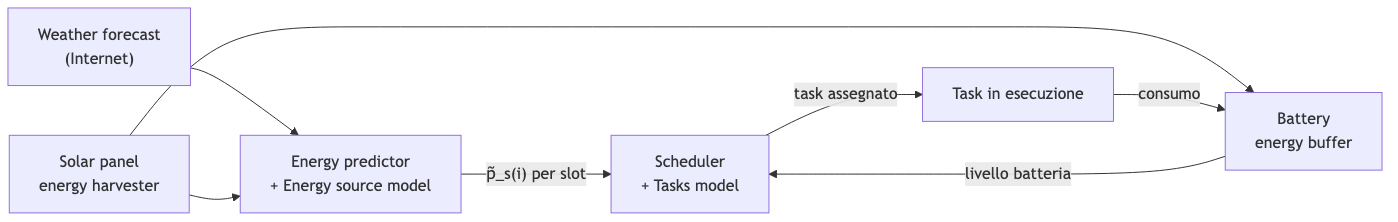
\includegraphics[keepaspectratio,alt={Architettura del sistema task-based che mostra il flusso delle previsioni, la schedulazione e il consumo della batteria}]{images/mermaid-04-gestione-energetica-03.png}}
\caption{Architettura del sistema task-based che mostra il flusso delle
previsioni, la schedulazione e il consumo della batteria}
\end{figure}

\emph{Fig. --- Architettura del sistema task-based.}

\subsection{Formulazione e Programmazione
Dinamica}\label{formulazione-e-programmazione-dinamica}

Lo scheduler assegna \textbf{esattamente un task per slot}
(\(x_{i,j}=1\)), massimizzando l'utility totale
\(\sum \sum x_{i,j} u_j\) sotto i vincoli che la batteria non si
esaurisca mai e alla fine della giornata il livello non sia inferiore a
quello iniziale (\(B(k+1) \ge B(1)\)).

Il problema è \textbf{NP-Hard} ma si risolve in modo esatto in tempo
\textbf{pseudo-polinomiale} usando la programmazione dinamica,
esplorando a ritroso (backward) gli slot \(i\) e i livelli di batteria
discretizzati \(b\):

\[opt(i, b) = \max_{j=1,\ldots,n} \{u_j + opt(i+1, B^j(i+1)) : B^j(i+1) \geq B_{min}\}\]

La complessità temporale è \(O(k \cdot \text{BatteryLevels})\).
Discretizzando la batteria in \textasciitilde200 livelli con l'ADC, il
problema si risolve in frazioni di secondo anche su Arduino, risultando
perfetto per una schedulazione giornaliera.

\begin{figure}
\centering
\pandocbounded{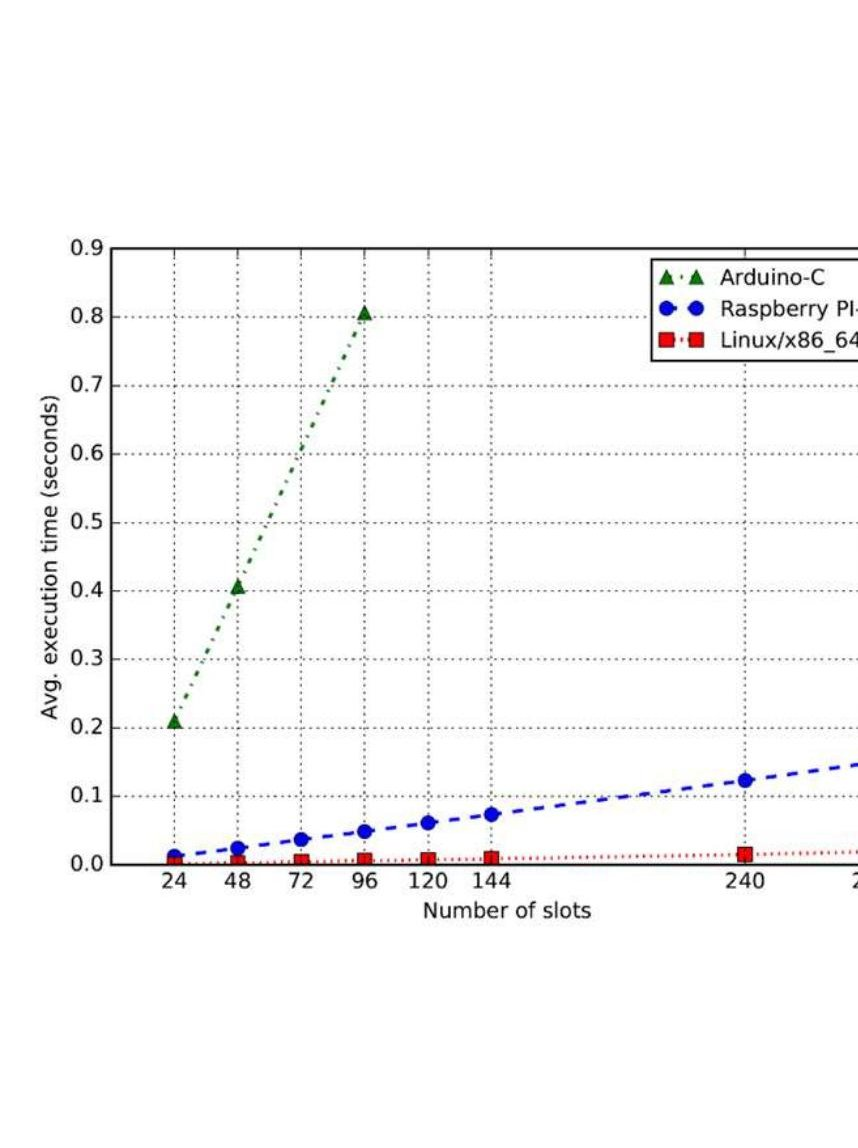
\includegraphics[keepaspectratio,alt={Grafico tempo di esecuzione}]{images/lezione-28-kansal-problem-e-energy-neutrality-img-05.jpg}}
\caption{Grafico tempo di esecuzione}
\end{figure}

\begin{figure}
\centering
\pandocbounded{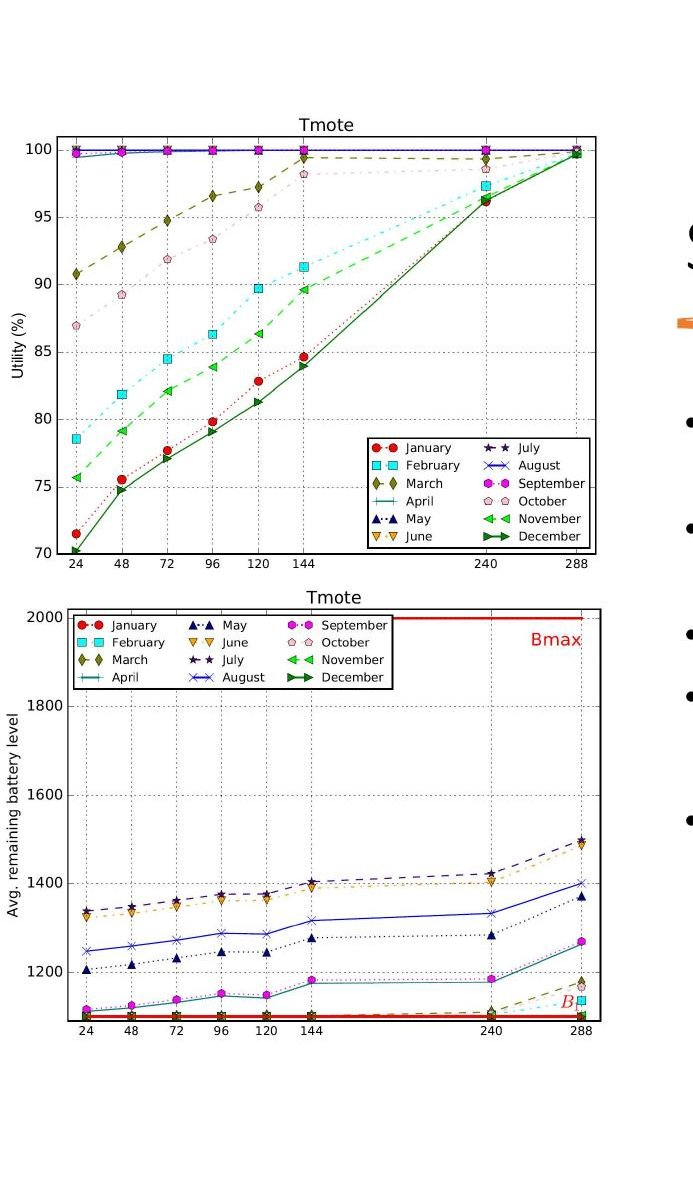
\includegraphics[keepaspectratio,alt={Utility e livello medio batteria}]{images/lezione-28-kansal-problem-e-energy-neutrality-img-06.jpg}}
\caption{Utility e livello medio batteria}
\end{figure}

\begin{figure}
\centering
\pandocbounded{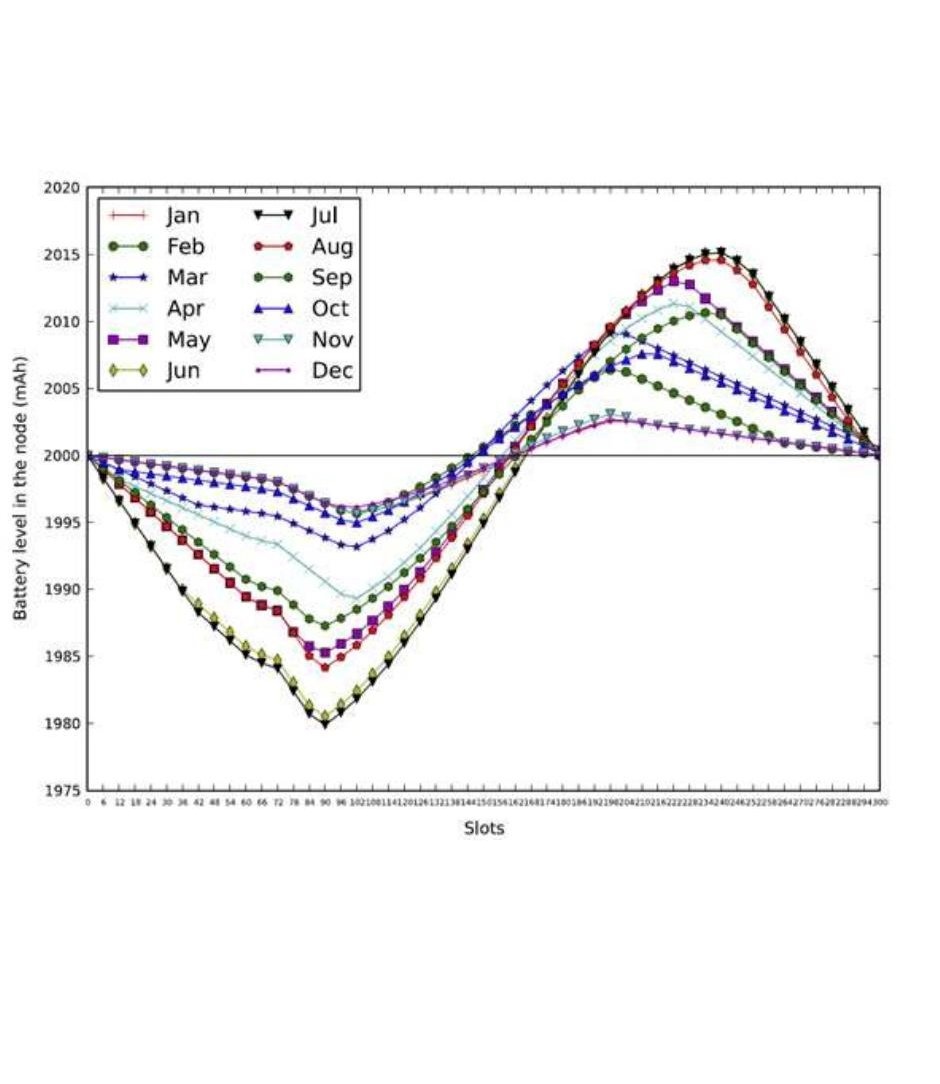
\includegraphics[keepaspectratio,alt={Livello batteria durante il giorno}]{images/lezione-28-kansal-problem-e-energy-neutrality-img-07.jpg}}
\caption{Livello batteria durante il giorno}
\end{figure}

\begin{center}\rule{0.5\linewidth}{0.5pt}\end{center}

\section{Riepilogo}\label{riepilogo}

\begin{figure}
\centering
\pandocbounded{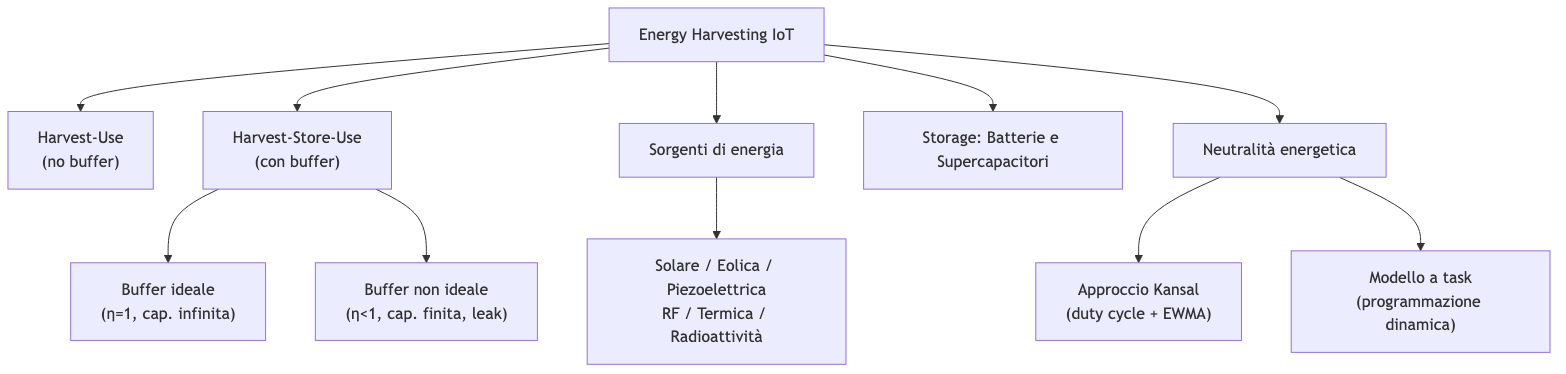
\includegraphics[keepaspectratio,alt={Mappa concettuale complessiva dei concetti relativi all'Energy Harvesting e neutralità energetica}]{images/mermaid-04-gestione-energetica-04.png}}
\caption{Mappa concettuale complessiva dei concetti relativi all'Energy
Harvesting e neutralità energetica}
\end{figure}

\begin{calloutquestion}{Possibili domande d’esame}

- Qual è la differenza tra architettura Harvest-Use e Harvest-Store-Use?
- Scrivi le equazioni di conservazione dell'energia per un buffer non
ideale. - Classifica le sorgenti per controllabilità e prevedibilità. -
Come si stima la carica via ADC? Derivare la formula. - Quali sono le
tre condizioni sufficienti del Teorema di Kansal per l'energy
neutrality? - Descrivi l'algoritmo di Kansal nei casi di sovraproduzione
e sottoproduzione con un esempio. - Descrivi la funzione utility
\(u(dc)\) in Kansal e calcola \(\alpha, \beta\). - Cos'è il modello a
task, come migliora Kansal e come risolve la complessità NP-Hard
(Dynamic Programming)?

\end{calloutquestion}

\newpage

\chapter{05 - Preparazione Esame Orale}\label{preparazione-esame-orale}

Documento di preparazione all'esame orale del corso \textbf{Mobile and
Cyber-Physical Systems}, modulo del Prof.~Stefano Chessa. Per ogni
schema del documento originale viene fornita una risposta dettagliata,
corredata dell'immagine di riferimento e dei link alle lezioni
pertinenti.

\begin{center}\rule{0.5\linewidth}{0.5pt}\end{center}

\section{Interoperabilità}\label{interoperabilituxe0}

\begin{figure}
\centering
\pandocbounded{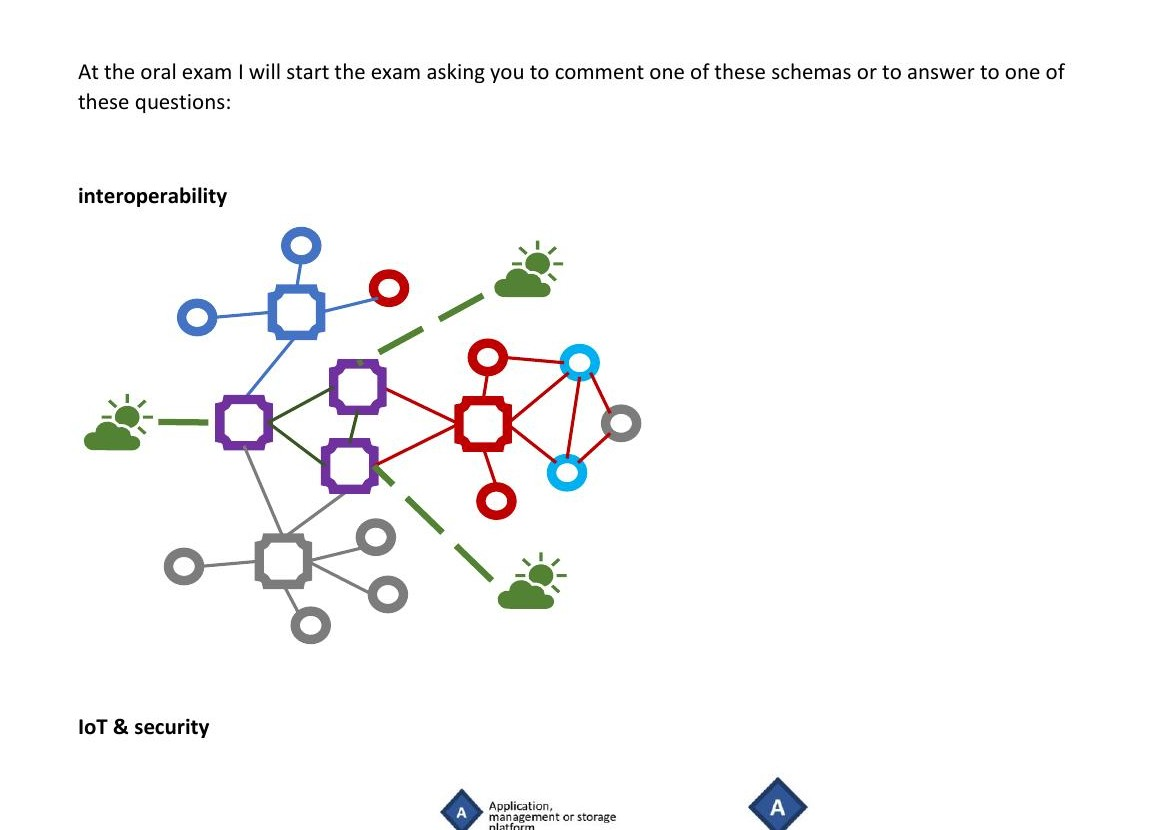
\includegraphics[keepaspectratio]{images/exam-chessa-interoperability.jpg}}
\caption{Rete IoT eterogenea: dispositivi di produttori diversi (colori
diversi) comunicano attraverso gateway di integrazione.}
\end{figure}

Lo schema mostra una rete in cui dispositivi appartenenti a ecosistemi
diversi (rappresentati con colori diversi) devono comunicare tra loro.
Il problema fondamentale è l'\textbf{interoperabilità}.

Il percorso storico delle soluzioni IoT ``dal basso'' porta spesso alla
creazione di \textbf{vertical silos}: sistemi proprietari in cui i
dispositivi di un fornitore comunicano solo con l'infrastruttura dello
stesso produttore. Questa strategia risponde a un preciso modello di
business chiamato \textbf{vendor lock-in}, che costringe il cliente a
restare nell'ecosistema del fornitore pena una costosa migrazione.

La soluzione naturale è l'adozione di \textbf{standard condivisi}
(Wi-Fi, ZigBee, Bluetooth, ecc.), ma la proliferazione degli standard
sposta il problema al livello middleware e applicativo: oggi coesistono
MQTT, CoAP, LWM2M e molti altri protocolli applicativi, incompatibili
tra loro.

Per gestire questa eterogeneità si ricorre agli
\textbf{application-level gateway}, che non si limitano a tradurre
protocolli di basso livello ma mappano comportamenti applicativi
differenti, operando come interpreti semantici tra ecosistemi.

Le architetture IoT si classificano in quattro tipi:

{\def\LTcaptype{none} % do not increment counter
\begin{longtable}[]{@{}llll@{}}
\toprule\noalign{}
Tipo & Fornitore & Protocollo & Gateway? \\
\midrule\noalign{}
\endhead
\bottomrule\noalign{}
\endlastfoot
A & Unico & Unico & No \\
B & Multiplo & Unico condiviso & No / minimale \\
C & Multiplo & Diversi & Sì --- traduzione \\
D & Multiplo & Eterogenei distribuiti & Sì --- gateway multipli \\
\end{longtable}
}

All'aumentare della complessità da A a D, il gateway deve gestire un
numero esponenziale di mappature tra protocolli.

\begin{calloutnote}{Riferimento}

{[}{[}Lezione 3 - Interoperabilità e Standard{]}{]}

\end{calloutnote}

\begin{center}\rule{0.5\linewidth}{0.5pt}\end{center}

\section{IoT \& Security}\label{iot-security}

\begin{figure}
\centering
\pandocbounded{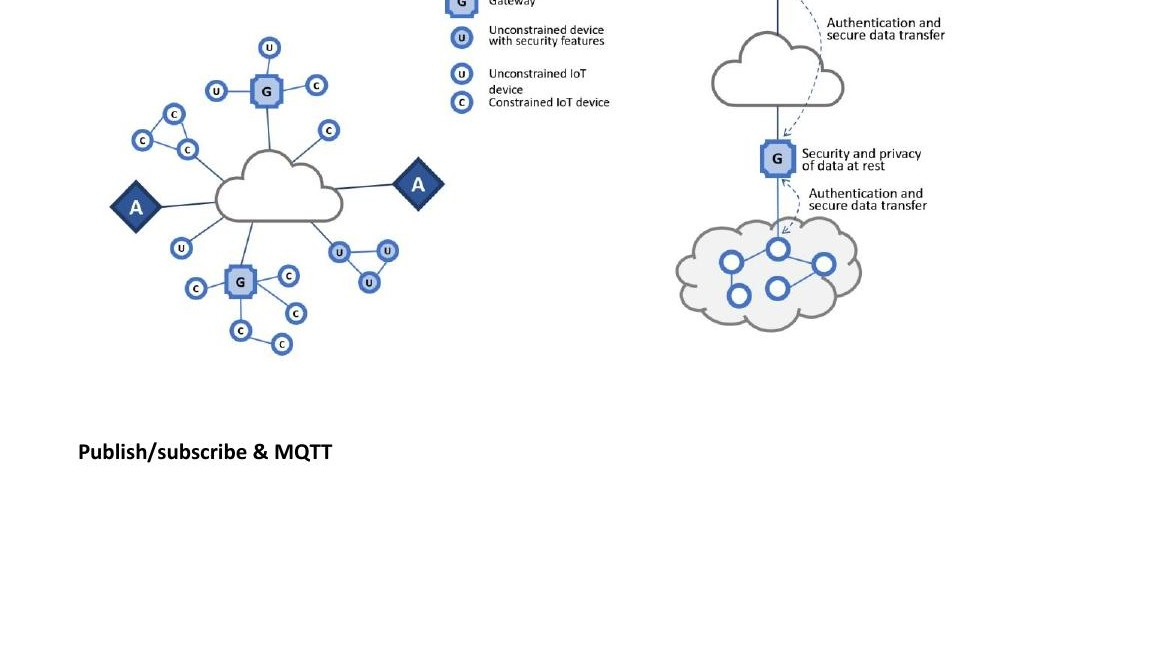
\includegraphics[keepaspectratio]{images/exam-chessa-iot-security.jpg}}
\caption{Architettura di sicurezza IoT: dispositivi vincolati (C),
gateway (G), applicazioni (A) e relative misure di sicurezza per ogni
livello.}
\end{figure}

Lo schema mostra un'architettura IoT a strati in cui la sicurezza deve
essere garantita a ogni livello: tra dispositivi periferici e gateway
(autenticazione + trasferimento sicuro), e tra gateway e
cloud/applicazione (sicurezza dei dati a riposo + autenticazione).

I dispositivi IoT sono spesso sistemi embedded economici, prodotti con
forti incentivi a ridurre costi e tempi di immissione sul mercato, a
discapito della sicurezza. La conseguenza sono centinaia di milioni di
dispositivi vulnerabili, privi di meccanismi di patching efficaci.

La raccomandazione \textbf{ITU-T Y.2066} definisce tre aree fondamentali
di sicurezza:

\begin{enumerate}
\def\labelenumi{\arabic{enumi}.}
\tightlist
\item
  \textbf{Sicurezza della comunicazione} --- riservatezza e integrità
  dei dati in transito tra dispositivi e piattaforme.
\item
  \textbf{Sicurezza della gestione dei dati} --- protezione di
  riservatezza e integrità quando i dati sono archiviati o elaborati
  (\emph{data at rest}).
\item
  \textbf{Sicurezza della fornitura del servizio} --- prevenzione di
  accessi non autorizzati e protezione della privacy degli utenti.
\end{enumerate}

A questi si aggiungono l'\textbf{autenticazione mutua} (entrambe le
parti si verificano reciprocamente, più robusta dell'autenticazione a
una via) e la capacità di audit di sicurezza.

Il \textbf{gateway} gioca un ruolo centrale: - Gestisce identificazione
e autenticazione di ogni dispositivo connesso. - Protegge la privacy dei
dispositivi periferici. - Supporta manutenzione, aggiornamento firmware
e autodiagnosi remota. - Applica policy di configurazione dinamiche.

\begin{calloutwarning}{Dispositivi vincolati e limiti}

I \emph{constrained devices} spesso non dispongono di hardware
crittografico dedicato, rendendo impraticabile la cifratura dei dati
archiviati. Con il \emph{Massive IoT}, la privacy diventa critica per la
grande mole di dati sensibili (medici, posizione, abitudini) raccolti.

\end{calloutwarning}

\begin{calloutnote}{Riferimento}

{[}{[}Lezione 3 - Interoperabilità e Standard{]}{]} (sezione sicurezza)

\end{calloutnote}

\begin{center}\rule{0.5\linewidth}{0.5pt}\end{center}

\section{Publish/Subscribe \& MQTT}\label{publishsubscribe-mqtt}

\begin{figure}
\centering
\pandocbounded{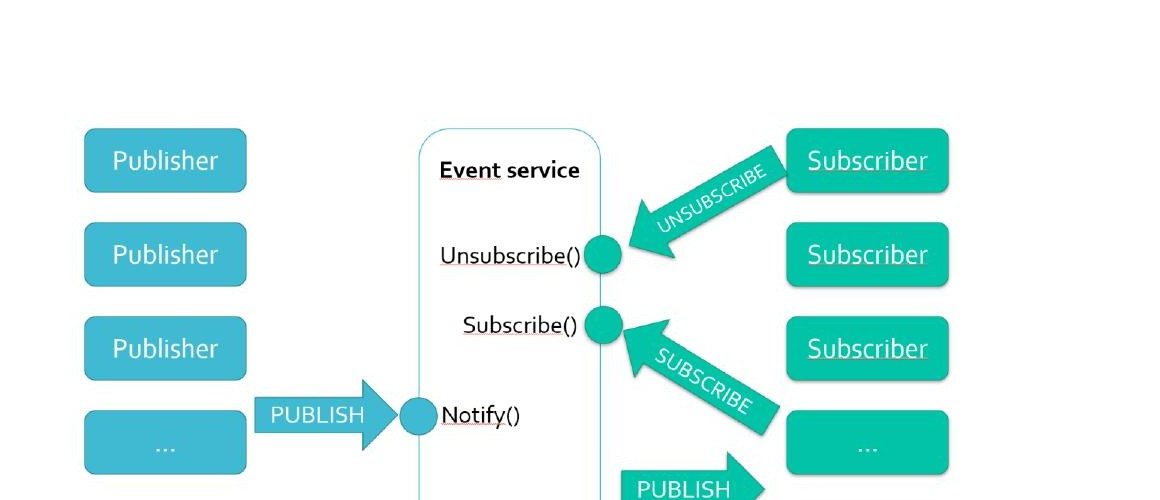
\includegraphics[keepaspectratio]{images/exam-chessa-mqtt-pubsub.jpg}}
\caption{Il paradigma publish/subscribe: i publisher inviano messaggi al
broker tramite PUBLISH; i subscriber si registrano (SUBSCRIBE) e
ricevono notifiche (PUBLISH dal broker); possono anche disdire
(UNSUBSCRIBE).}
\end{figure}

Il paradigma \textbf{publish/subscribe} è il cuore di MQTT. A differenza
del modello client/server, il pub/sub è \emph{loosely coupled} grazie a
tre forme di disaccoppiamento:

\begin{itemize}
\tightlist
\item
  \textbf{Space decoupling}: publisher e subscriber non si conoscono,
  non condividono IP né porta.
\item
  \textbf{Time decoupling}: non devono essere attivi contemporaneamente.
\item
  \textbf{Synchronization decoupling}: le operazioni non sono bloccanti.
\end{itemize}

Il \textbf{broker} è il server dell'infrastruttura: riceve tutti i
messaggi, li filtra per topic, li distribuisce ai subscriber
interessati. Le operazioni fondamentali sono quattro: \emph{Publish},
\emph{Subscribe}, \emph{Notify}, \emph{Unsubscribe}.

\textbf{MQTT} (\emph{Message Queuing Telemetry Transport}) implementa
pub/sub con filtraggio basato su \textbf{topic} --- stringhe gerarchiche
separate da \texttt{/} (es.
\texttt{home/firstfloor/bedroom/temperature}). I subscriber possono
usare wildcard: - \texttt{+} sostituisce un singolo livello:
\texttt{home/+/temperature} - \texttt{\#} sostituisce tutti i livelli
successivi: \texttt{home/\#}

MQTT opera su TCP (porta 1883, o 8883 con TLS) e concentra la
complessità sul broker, mantenendo i client semplici. È \emph{data
agnostic}: il payload può essere binario, testo, JSON o XML.

\begin{calloutnote}{Riferimento}

{[}{[}Lezione 4 - MQTT Part 1{]}{]}

\end{calloutnote}

\begin{center}\rule{0.5\linewidth}{0.5pt}\end{center}

\section{MQTT -- II (QoS 2)}\label{mqtt-ii-qos-2}

\begin{figure}
\centering
\pandocbounded{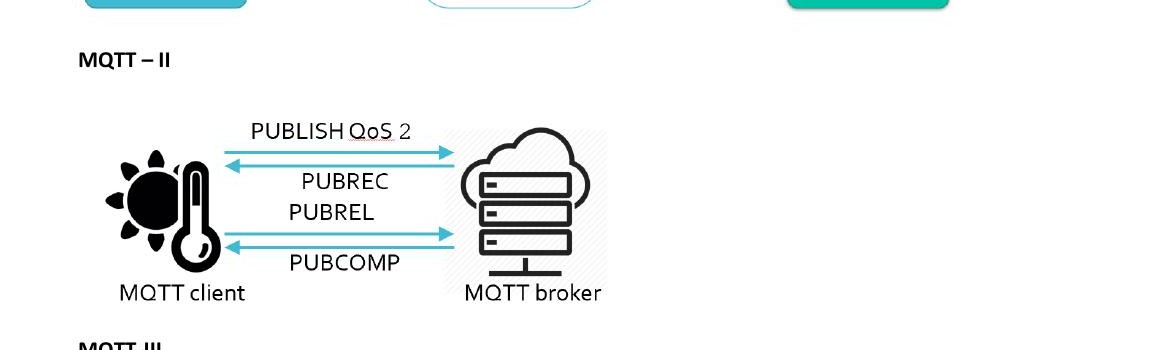
\includegraphics[keepaspectratio]{images/exam-chessa-mqtt-qos2.jpg}}
\caption{Handshake a quattro fasi del QoS 2 tra MQTT client e broker:
PUBLISH → PUBREC → PUBREL → PUBCOMP.}
\end{figure}

MQTT definisce tre livelli di \textbf{Quality of Service}:

{\def\LTcaptype{none} % do not increment counter
\begin{longtable}[]{@{}
  >{\raggedright\arraybackslash}p{(\linewidth - 6\tabcolsep) * \real{0.2432}}
  >{\raggedright\arraybackslash}p{(\linewidth - 6\tabcolsep) * \real{0.1622}}
  >{\raggedright\arraybackslash}p{(\linewidth - 6\tabcolsep) * \real{0.2703}}
  >{\raggedright\arraybackslash}p{(\linewidth - 6\tabcolsep) * \real{0.3243}}@{}}
\toprule\noalign{}
\begin{minipage}[b]{\linewidth}\raggedright
Livello
\end{minipage} & \begin{minipage}[b]{\linewidth}\raggedright
Nome
\end{minipage} & \begin{minipage}[b]{\linewidth}\raggedright
Garanzia
\end{minipage} & \begin{minipage}[b]{\linewidth}\raggedright
Meccanismo
\end{minipage} \\
\midrule\noalign{}
\endhead
\bottomrule\noalign{}
\endlastfoot
QoS 0 & At most once & Nessuna & Nessun ACK \\
QoS 1 & At least once & Almeno una consegna & PUBACK (possibili
duplicati) \\
QoS 2 & Exactly once & Esattamente una consegna & 4-way handshake \\
\end{longtable}
}

\textbf{QoS 2} è il livello più affidabile. Il handshake a quattro fasi
serve a evitare sia la perdita che la duplicazione:

\begin{enumerate}
\def\labelenumi{\arabic{enumi}.}
\tightlist
\item
  \textbf{PUBLISH}: il client invia il messaggio al broker (con
  packetId).
\item
  \textbf{PUBREC} (\emph{Publish Received}): il broker conferma la
  ricezione e memorizza il messaggio.
\item
  \textbf{PUBREL} (\emph{Publish Release}): il client autorizza il
  broker a procedere con la consegna effettiva.
\item
  \textbf{PUBCOMP} (\emph{Publish Complete}): il broker conferma che la
  consegna ai subscriber è avvenuta e il messaggio può essere eliminato.
\end{enumerate}

Il PUBREC garantisce che il messaggio non vada perso; PUBREL + PUBCOMP
garantiscono che non venga consegnato due volte. Due fasi non sarebbero
sufficienti perché, se il broker consegnasse immediatamente al PUBLISH
senza aspettare PUBREL, e il client ritrasmettesse credendo di non aver
ricevuto PUBREC, si avrebbero duplicati.

\begin{calloutnote}{Riferimento}

{[}{[}Lezione 4 - MQTT Part 1{]}{]}

\end{calloutnote}

\begin{center}\rule{0.5\linewidth}{0.5pt}\end{center}

\section{MQTT-III --- Topic, Sessioni, Retained Messages, Last Will \&
Keep
Alive}\label{mqtt-iii-topic-sessioni-retained-messages-last-will-keep-alive}

\subsection{Come il broker filtra i messaggi e cosa sono i
topic}\label{come-il-broker-filtra-i-messaggi-e-cosa-sono-i-topic}

Il broker usa il \textbf{filtraggio basato su topic} (topic-based
filtering): ogni messaggio PUBLISH porta un topic; il broker lo
confronta con le sottoscrizioni attive e lo consegna ai subscriber che
corrispondono. I topic sono stringhe gerarchiche; le wildcard \texttt{+}
e \texttt{\#} permettono iscrizioni a insiemi di topic. Il broker non
ispeziona il payload (a differenza del content-based filtering), il che
consente la cifratura end-to-end.

\subsection{Sessioni Persistenti}\label{sessioni-persistenti-1}

Quando un dispositivo IoT si disconnette (per sleep, copertura persa,
reset), rischia di perdere le sottoscrizioni attive e i messaggi
pubblicati durante l'assenza. Le \textbf{persistent session} risolvono
questo: impostando \texttt{cleanSession\ =\ false} nel CONNECT, il
broker conserva per quel \texttt{clientId}: - Tutte le sottoscrizioni
attive - I messaggi non consegnati con QoS 1 o 2 - I messaggi in attesa
di completamento del flusso QoS 2

Alla riconnessione con lo stesso \texttt{clientId}, la sessione viene
ripristinata automaticamente. Il broker segnala la presenza di una
sessione precedente tramite il flag \emph{Session Present} nel CONNACK.

\subsection{Retained Messages}\label{retained-messages}

Nel pub/sub classico, un nuovo subscriber non sa quando arriverà il
primo messaggio. I \textbf{retained message} risolvono questo: un
messaggio pubblicato con \texttt{retainFlag\ =\ true} viene conservato
dal broker (uno per topic). Ogni nuovo subscriber riceve immediatamente
l'ultimo messaggio trattenuto al momento dell'iscrizione, senza
aspettare la prossima pubblicazione.

\begin{callouttip}{Pattern potente}

Un dispositivo pubblica il proprio stato (\texttt{"ON"}) come retained
message. Configura anche un testamento con payload \texttt{"OFF"} e
retain flag attivo sullo stesso topic. Se va in crash, il broker
pubblica automaticamente \texttt{"OFF"} come retained message --- tutti
i client (connessi e futuri) vedono lo stato corretto.

\end{callouttip}

\subsection{Last Will \& Testament}\label{last-will-testament}

Quando un dispositivo si disconnette \emph{normalmente} (DISCONNECT),
può notificare gli altri esplicitamente. Per le \textbf{disconnessioni
anomale} (crash, timeout, interruzione di rete) non esiste tale
possibilità. Il \textbf{Last Will \& Testament} consiste in un messaggio
pre-configurato consegnato al broker al momento del CONNECT: se il
broker rileva una disconnessione anomala, pubblica quel messaggio
automaticamente. Il testamento ha topic, payload, QoS e retained flag
propri.

Il broker invia il testamento quando: errore di I/O sulla connessione,
mancato invio di PINGREQ entro il keep alive, chiusura brusca TCP senza
DISCONNECT, o chiusura forzata per errore di protocollo. Se il client si
disconnette con DISCONNECT regolare, il testamento viene scartato.

\subsection{Keep Alive}\label{keep-alive-1}

TCP può mantenere una connessione apparentemente attiva anche quando il
peer è irraggiungibile. Il \textbf{Keep Alive} risolve: il client
dichiara un intervallo (campo a 16 bit nel CONNECT) entro cui si impegna
a inviare almeno un pacchetto. Se non lo fa, il broker chiude la
connessione e invia il testamento. Il client invia \textbf{PINGREQ} se
non ha altro traffico; il broker risponde con \textbf{PINGRESP}. Il
valore \texttt{0} disabilita il meccanismo.

\begin{calloutnote}{Riferimento}

{[}{[}Lezione 4 - MQTT Part 1{]}{]}, {[}{[}Lezione 8 - MQTT Part 2{]}{]}

\end{calloutnote}

\begin{center}\rule{0.5\linewidth}{0.5pt}\end{center}

\section{ZigBee - I (Join through
Association)}\label{zigbee---i-join-through-association}

\begin{figure}
\centering
\pandocbounded{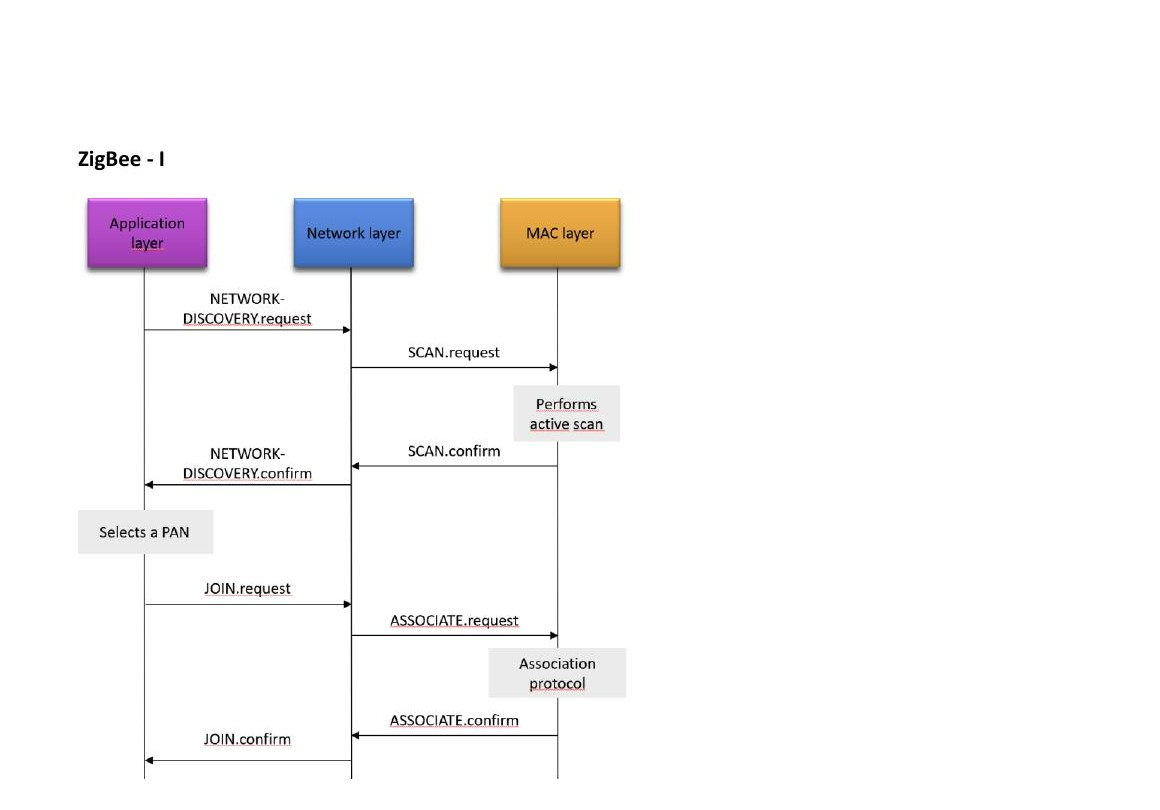
\includegraphics[keepaspectratio]{images/exam-chessa-zigbee-join.jpg}}
\caption{Sequenza di primitives tra Application Layer, Network Layer e
MAC Layer durante il processo di join di un dispositivo ZigBee.}
\end{figure}

Lo schema mostra il processo con cui un dispositivo si unisce a una rete
ZigBee esistente attraverso il meccanismo di \textbf{associazione}. Si
tratta di un'interazione a tre livelli (Application, Network, MAC)
tramite service primitives.

La sequenza è:

\begin{enumerate}
\def\labelenumi{\arabic{enumi}.}
\tightlist
\item
  \textbf{Application layer} emette \texttt{NETWORK-DISCOVERY.request}
  al Network Layer.
\item
  \textbf{Network Layer} emette \texttt{SCAN.request} al MAC: viene
  eseguito un active scan per trovare le PAN disponibili.
\item
  \textbf{MAC} esegue lo scan e risponde con \texttt{SCAN.confirm}.
\item
  \textbf{Network Layer} risponde all'applicazione con
  \texttt{NETWORK-DISCOVERY.confirm}, che elenca le PAN trovate.
\item
  \textbf{Application layer} sceglie una PAN e invia
  \texttt{JOIN.request} al Network Layer.
\item
  \textbf{Network Layer} seleziona un nodo genitore P e avvia il
  protocollo di associazione MAC tramite \texttt{ASSOCIATE.request}.
\item
  \textbf{MAC} esegue il protocollo di associazione: il
  coordinatore/router assegna un \textbf{indirizzo breve a 16 bit} al
  nuovo dispositivo.
\item
  \textbf{MAC} risponde con \texttt{ASSOCIATE.confirm} → \textbf{Network
  Layer} risponde con \texttt{JOIN.confirm} all'applicazione.
\end{enumerate}

Nelle reti a stella, P è necessariamente il coordinatore. Nelle reti ad
albero o mesh, P può essere qualsiasi router raggiungibile.

\begin{calloutnote}{Riferimento}

{[}{[}Lezione 9 - The ZigBee Standard Part 1{]}{]}

\end{calloutnote}

\begin{center}\rule{0.5\linewidth}{0.5pt}\end{center}

\section{ZigBee -- II (Application Layer
Stack)}\label{zigbee-ii-application-layer-stack}

\begin{figure}
\centering
\pandocbounded{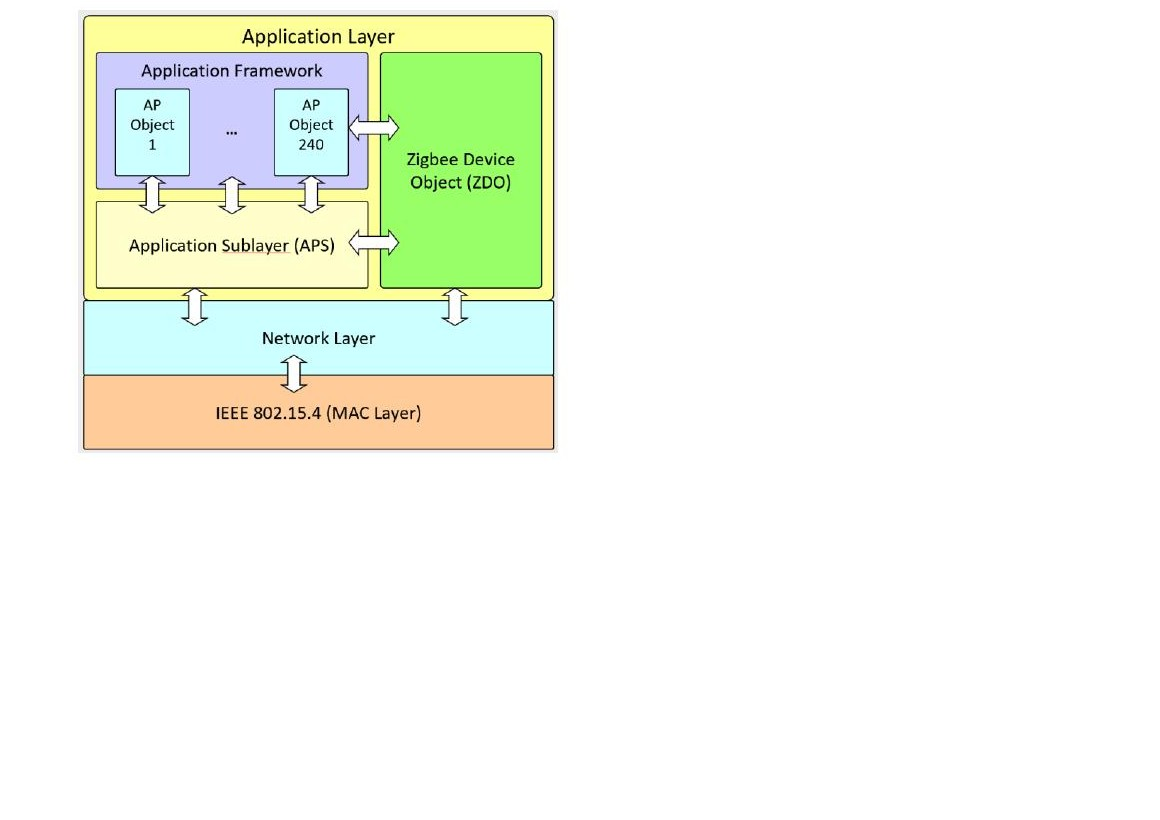
\includegraphics[keepaspectratio]{images/exam-chessa-zigbee-applayer.jpg}}
\caption{Stack protocollare ZigBee: dall'IEEE 802.15.4 (MAC) fino
all'Application Layer, con Application Framework, ZDO e APS.}
\end{figure}

ZigBee aggiunge sopra IEEE 802.15.4 (PHY + MAC) due livelli:
\textbf{Network Layer} e \textbf{Application Layer}. Il livello
applicativo si compone di tre elementi:

\textbf{Application Framework}: ospita fino a 240 \textbf{Application
Objects (APO)}, ciascuno associato a un endpoint (numerato da 1 a 240).
Ogni APO è identificato univocamente dalla coppia
\texttt{\textless{}indirizzo\ di\ rete,\ endpoint\textgreater{}}. Più
APO sullo stesso dispositivo possono corrispondere ad applicazioni
diverse che operano simultaneamente.

\textbf{ZigBee Device Object (ZDO)}: occupa l'endpoint 0 ed è la
componente gestionale del nodo. Fornisce: - Device \& Service Discovery
(trova altri nodi e i loro servizi) - Binding Management (crea/modifica
le binding table dell'APS) - Network Management (gestisce join/leave e
routing table)

\textbf{Application Support Sublayer (APS)}: fa da intermediario tra
APO/ZDO e il Network Layer. Fornisce: - \emph{Data Service}:
trasmissione messaggi con acknowledgment end-to-end - \emph{Binding
Service}: creazione di connessioni logiche tra endpoint - \emph{Group
Management}: indirizzamento multicast tramite Group Table

L'APS filtra i pacchetti per endpoint e profile ID, scartando quelli non
destinati ad applicazioni registrate.

\begin{calloutnote}{Riferimento}

{[}{[}Lezione 9 - The ZigBee Standard Part 1{]}{]}, {[}{[}Lezione 12 -
Application Layer of ZigBee{]}{]}

\end{calloutnote}

\begin{center}\rule{0.5\linewidth}{0.5pt}\end{center}

\section{ZigBee - III (Topologie di
Rete)}\label{zigbee---iii-topologie-di-rete}

\begin{figure}
\centering
\pandocbounded{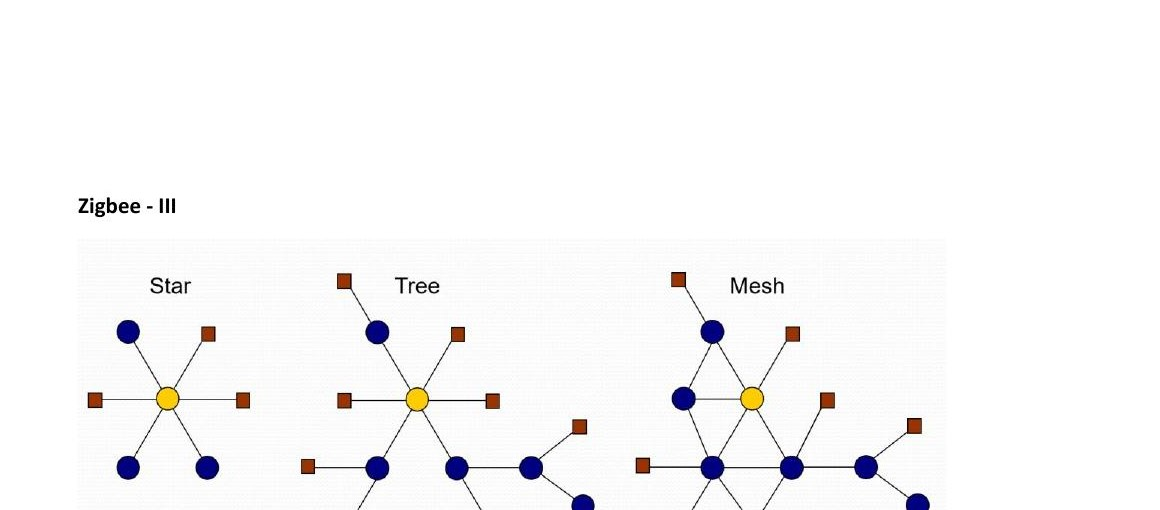
\includegraphics[keepaspectratio]{images/exam-chessa-zigbee-topologies.jpg}}
\caption{Le tre topologie ZigBee: Star (sinistra), Tree (centro), Mesh
(destra). Nodo giallo = coordinatore, nodi blu = router, nodi rossi =
end-device.}
\end{figure}

ZigBee supporta tre topologie di rete gestite dal Network Layer:

\textbf{Star (Stella)}: tutti i dispositivi comunicano direttamente con
il coordinatore. Si mappa direttamente sulla struttura IEEE 802.15.4 e
supporta il meccanismo del superframe/beacon. Semplice ma non scalabile:
ogni dispositivo deve essere nel raggio radio del coordinatore.

\textbf{Tree (Albero)}: il coordinatore è la radice, i router sono nodi
interni, gli end-device sono foglie. Può usare il superframe. Il routing
segue la struttura gerarchica (tree routing): i pacchetti salgono verso
la radice e poi scendono verso la destinazione. Il vantaggio è la
semplicità; lo svantaggio è la rigidità e i percorsi spesso subottimali.

\textbf{Mesh}: topologia più flessibile in cui i router possono
comunicare direttamente tra loro indipendentemente dalla struttura ad
albero. Usa mesh routing (ispirato ad AODV): se non esiste un'entry
nella routing table, viene avviato il Route Discovery Protocol
(broadcast RREQ, unicast RREP). Non supporta il beaconing. È più
robusto: percorsi alternativi sono disponibili se un link cade.

\begin{callouttip}{Coesistenza}

Tree routing e Mesh routing possono coesistere nella stessa rete: ogni
router mantiene sia la logica ad albero che la routing table mesh,
passando dinamicamente dall'uno all'altro.

\end{callouttip}

\begin{calloutnote}{Riferimento}

{[}{[}Lezione 9 - The ZigBee Standard Part 1{]}{]}

\end{calloutnote}

\begin{center}\rule{0.5\linewidth}{0.5pt}\end{center}

\section{ZigBee - IV (Indirizzamento ad
Albero)}\label{zigbee---iv-indirizzamento-ad-albero}

\begin{figure}
\centering
\pandocbounded{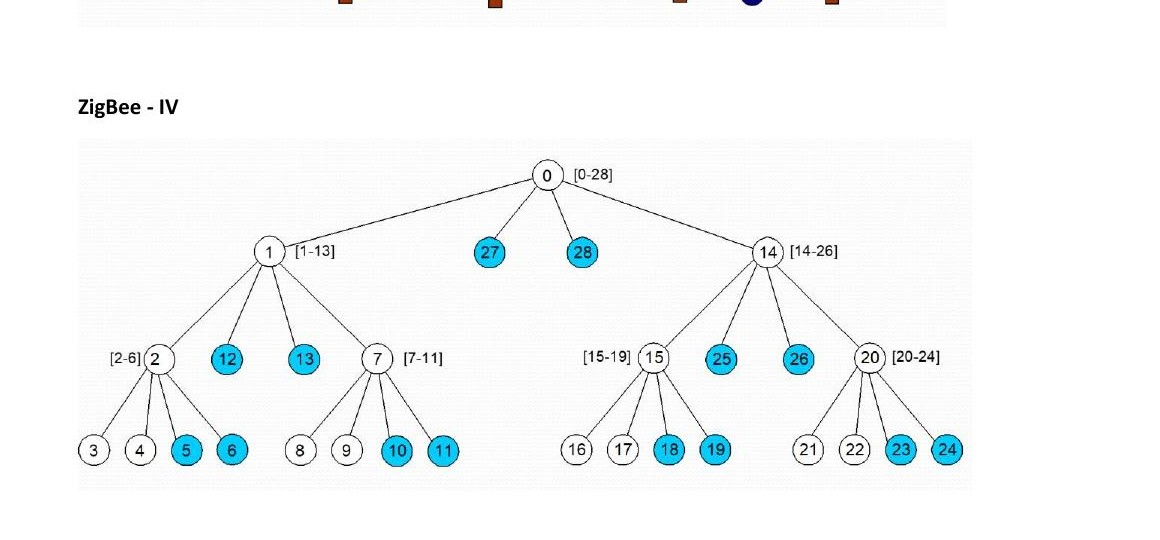
\includegraphics[keepaspectratio]{images/exam-chessa-zigbee-addrtree.jpg}}
\caption{Albero di indirizzi ZigBee con \(R_m=2\), \(D_m=2\), \(L_m=3\):
ogni nodo gestisce un intervallo di indirizzi calcolato con la formula
\(C_{skip}\).}
\end{figure}

ZigBee assegna gli indirizzi di rete in modo completamente
decentralizzato usando la struttura ad albero. Il coordinatore viene
configurato con tre parametri: - \(R_m\): massimo numero di router figli
per nodo - \(D_m\): massimo numero di end-device figli per nodo -
\(L_m\): profondità massima dell'albero

La dimensione del blocco di indirizzi assegnato a un router a profondità
\(d\) è:

\[C_{skip}(d) = \begin{cases} 1 & \text{se } d = L_m \\ 1 + R_m \cdot C_{skip}(d+1) + D_m & \text{altrimenti} \end{cases}\]

Se un router ha indirizzo \(A\) e si trova a profondità \(d\), i suoi
figli router ricevono: \(A+1\), \(A+1+C_{skip}(d+1)\),
\(A+1+2 \cdot C_{skip}(d+1)\), \ldots{} Gli end-device ricevono gli
indirizzi successivi a tutti i blocchi router.

\begin{callouttip}{Nell’immagine: R\_m=2, D\_m=2, L\_m=3}

\begin{itemize}
\tightlist
\item
  \(C_{skip}(3)=1\), \(C_{skip}(2)=5\), \(C_{skip}(1)=13\),
  \(C_{skip}(0)=29\)
\item
  Coordinator (addr=0) gestisce {[}0--28{]}; primo figlio router addr=1
  gestisce {[}1--13{]}; secondo figlio router addr=14 gestisce
  {[}14--26{]}; end-device 27 e 28.
\end{itemize}

\end{callouttip}

\textbf{Vantaggio}: completamente decentralizzato, nessun rischio di
collisione, nessun coordinamento distribuito necessario.

\textbf{Svantaggio}: rigido --- se un sottoalbero è saturo, nuovi
dispositivi non possono aggiungersi tramite quel nodo anche se ce ne
fosse necessità.

\begin{calloutnote}{Riferimento}

{[}{[}Lezione 9 - The ZigBee Standard Part 1{]}{]}

\end{calloutnote}

\begin{center}\rule{0.5\linewidth}{0.5pt}\end{center}

\section{ZigBee - V (Tabella APS / Binding
Table)}\label{zigbee---v-tabella-aps-binding-table}

\begin{figure}
\centering
\pandocbounded{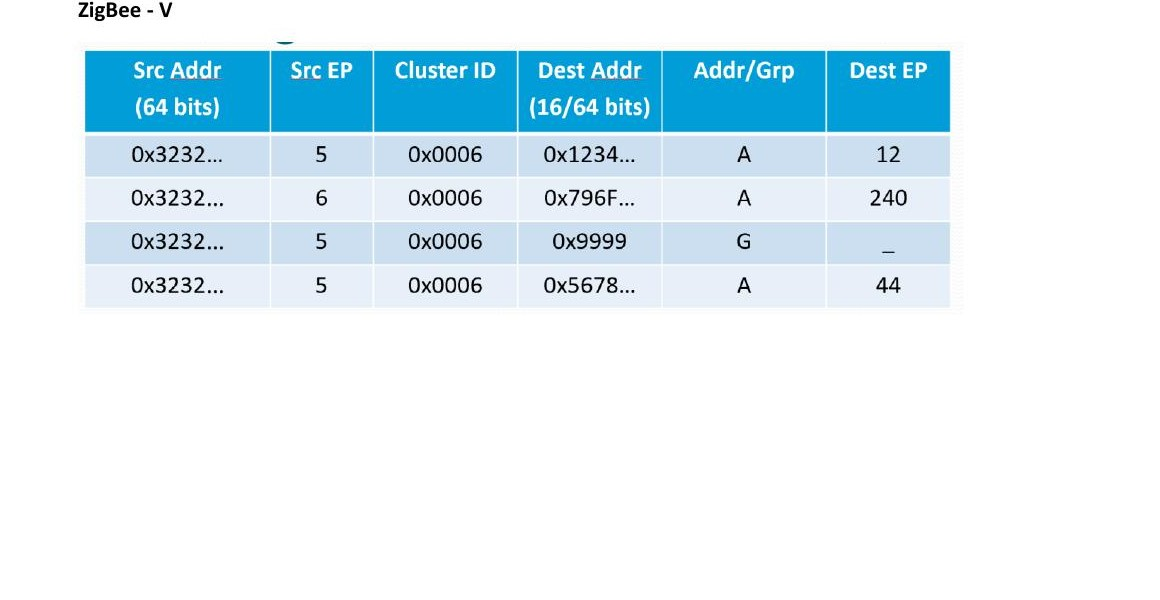
\includegraphics[keepaspectratio]{images/exam-chessa-zigbee-aps.jpg}}
\caption{Esempio di APS Binding Table: ogni entry mappa un endpoint
sorgente con cluster e destination address/endpoint.}
\end{figure}

La tabella mostra la \textbf{APS Binding Table}, il meccanismo con cui
ZigBee implementa l'\textbf{indirizzamento indiretto}. Un dispositivo
sorgente (che conosce solo il proprio endpoint e il cluster di
interesse) non ha bisogno di conoscere l'indirizzo di rete del
destinatario: consulta la binding table.

Le colonne della tabella sono: - \textbf{Src Addr (64 bit)}: indirizzo
MAC a 64 bit del dispositivo sorgente. - \textbf{Src EP}: endpoint
sorgente (1--240). - \textbf{Cluster ID}: il cluster di riferimento (es.
\texttt{0x0006} = OnOff Cluster). - \textbf{Dest Addr (16/64 bit)}:
indirizzo di destinazione (short 16 bit o MAC 64 bit). -
\textbf{Addr/Grp}: \texttt{A} = indirizzo unicast, \texttt{G} =
indirizzo di gruppo (multicast). - \textbf{Dest EP}: endpoint
destinazione (vuoto per i gruppi).

Nell'esempio, il dispositivo \texttt{0x3232...} endpoint 5 può inviare
messaggi: - All'indirizzo \texttt{0x1234...} endpoint 12 (unicast) -
All'indirizzo \texttt{0x796F...} endpoint 240 (unicast) - Al gruppo
\texttt{0x9999} (multicast, nessun endpoint specifico) - All'indirizzo
\texttt{0x5678...} endpoint 44 (unicast)

Questo meccanismo è fondamentale: se un dispositivo cambia indirizzo di
rete (dopo un reset), l'APS usa la \textbf{Address Map Table} (che
associa indirizzi 16-bit agli immutabili MAC 64-bit) per ripristinare i
binding automaticamente.

\begin{calloutnote}{Riferimento}

{[}{[}Lezione 12 - Application Layer of ZigBee{]}{]}

\end{calloutnote}

\begin{center}\rule{0.5\linewidth}{0.5pt}\end{center}

\section{ZigBee - VI (Cluster e Binding tra
Dispositivi)}\label{zigbee---vi-cluster-e-binding-tra-dispositivi}

\begin{figure}
\centering
\pandocbounded{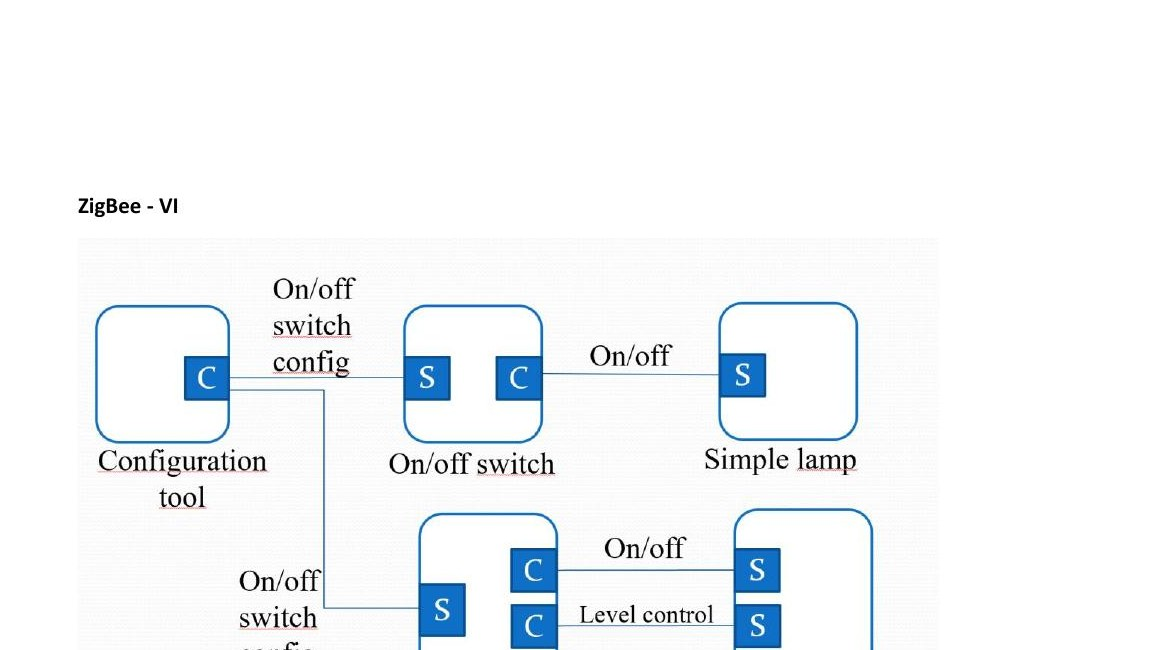
\includegraphics[keepaspectratio]{images/exam-chessa-zigbee-binding.jpg}}
\caption{Esempio di binding ZigBee: Configuration tool configura un
on/off switch, che controlla una Simple lamp e un Dimmer switch, il
quale controlla una Dimmable lamp.}
\end{figure}

Lo schema illustra come il \textbf{binding} ZigBee colleghi dispositivi
tramite cluster. Ogni rettangolo contiene le lettere C (Client) o S
(Server) per ciascun cluster supportato.

Un \textbf{Cluster} è una collezione di comandi e attributi che
definisce l'interfaccia per una funzionalità specifica. Ogni cluster ha
un ID a 16 bit (es. \texttt{0x0006} = OnOff, \texttt{0x0008} = Level
Control). Il cluster lato \textbf{server} ospita lo stato (attributi);
il lato \textbf{client} invia comandi.

Nell'esempio: - La \textbf{Configuration tool} (solo C) si lega
all'\textbf{On/off switch} (S+C) per configurarlo. - L'\textbf{On/off
switch} (come client) controla la \textbf{Simple lamp} (S = solo server
OnOff). - Il \textbf{Dimmer switch} (S+C) riceve configurazioni (S) e
controla la \textbf{Dimmable lamp} che implementa sia OnOff (S) che
Level Control (S).

Il binding è unidirezionale: si va da client a server. Viene creato
tramite \texttt{BIND.request} allo ZDO e memorizzato nella binding table
dell'APS. Un singolo client può essere legato a più server (fan-out).

\begin{calloutnote}{Riferimento}

{[}{[}Lezione 12 - Application Layer of ZigBee{]}{]}

\end{calloutnote}

\begin{center}\rule{0.5\linewidth}{0.5pt}\end{center}

\section{Duty Cycle - I (Calcolo del Duty
Cycle)}\label{duty-cycle---i-calcolo-del-duty-cycle}

\begin{figure}
\centering
\pandocbounded{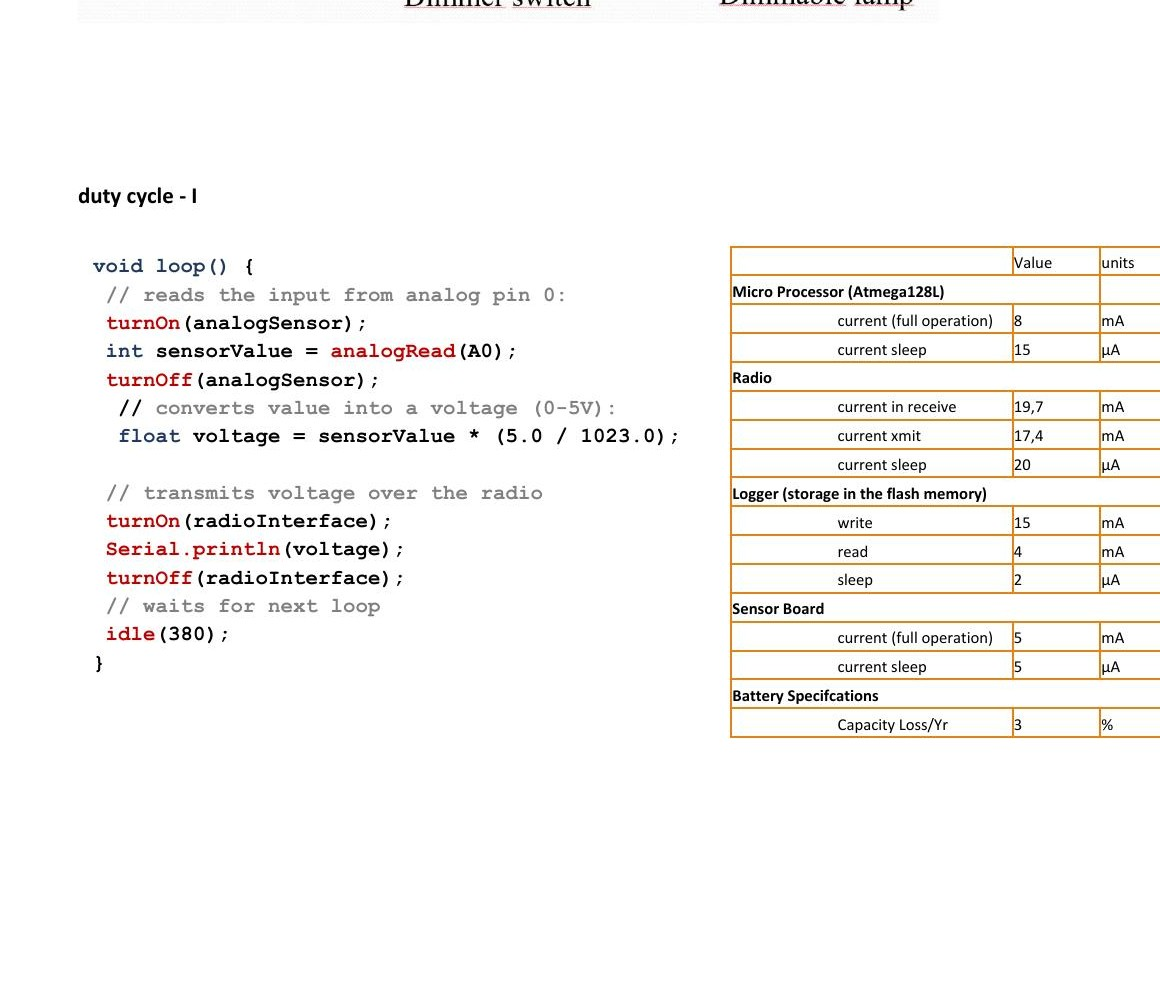
\includegraphics[keepaspectratio]{images/exam-chessa-dutycycle-code.jpg}}
\caption{Codice Arduino che implementa il duty cycling selettivo dei
componenti (sensore, radio) e tabella dei consumi in mA per componente e
stato.}
\end{figure}

Il \textbf{duty cycle} di un componente è la frazione di tempo in cui è
attivo rispetto al periodo totale. La strategia fondamentale di
risparmio energetico nei dispositivi IoT è attivare ogni componente
\textbf{solo quando strettamente necessario}.

Il codice mostra il pattern classico:

\begin{verbatim}
turnOn(analogSensor)   → sensore acceso solo durante lettura
analogRead(A0)         → lettura
turnOff(analogSensor)  → sensore spento

turnOn(radioInterface) → radio accesa solo durante trasmissione
Serial.println(voltage)
turnOff(radioInterface)

idle(380)              → MCU in sleep 380ms
\end{verbatim}

Usando i valori della tabella (es. Tmote Sky): - Processore attivo: 8
mA, sleep: 15 μA - Radio TX: 17.4 mA, RX: 19.7 mA, sleep: 20 μA -
Sensore: 5 mA, sleep: 5 μA

Se le operazioni di sensing + TX durano \textasciitilde20 ms e il ciclo
totale è 400 ms, il duty cycle della radio è 20/400 = 5\%. La corrente
media risultante è molto inferiore alla corrente di picco, estendendo la
vita della batteria di ordini di grandezza.

La perdita di capacità della batteria del 3\%/anno indica che anche con
battery standby c'è un degrado nel tempo.

\begin{calloutnote}{Riferimento}

{[}{[}Lezione 23 - Embedded Programming e Arduino{]}{]}

\end{calloutnote}

\begin{center}\rule{0.5\linewidth}{0.5pt}\end{center}

\section{Duty Cycle - II (Impatto sulla Vita della
Batteria)}\label{duty-cycle---ii-impatto-sulla-vita-della-batteria}

\begin{figure}
\centering
\pandocbounded{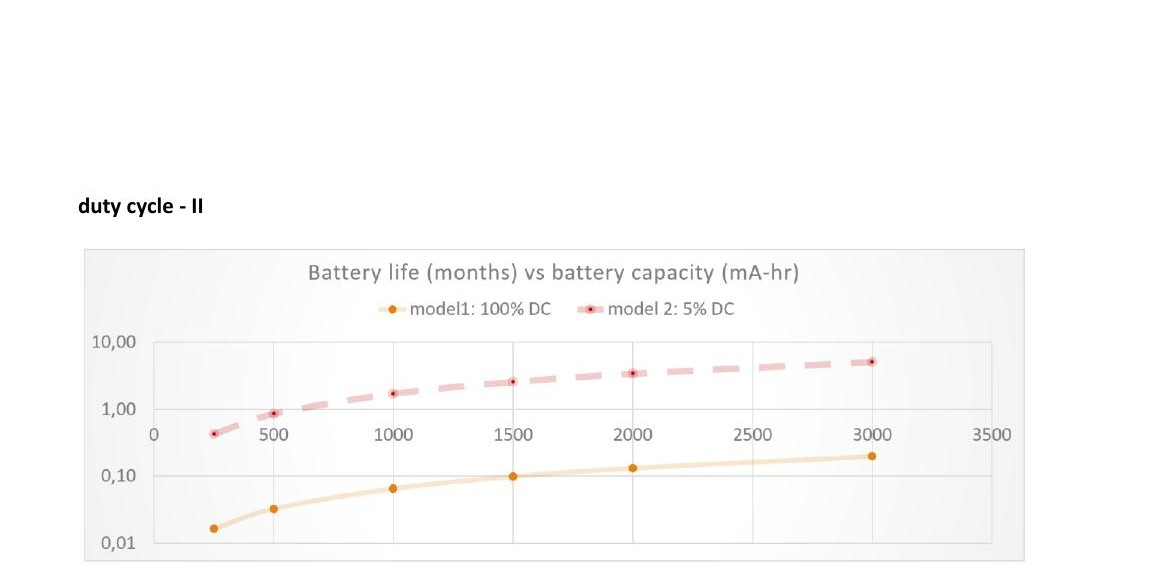
\includegraphics[keepaspectratio]{images/exam-chessa-dutycycle-graph.jpg}}
\caption{Grafico log-log: vita della batteria (mesi) vs capacità della
batteria (mAh) per duty cycle 100\% (model1) e 5\% (model2).}
\end{figure}

Il grafico mostra l'impatto del duty cycle sulla vita della batteria in
scala logaritmica. Due modelli a confronto:

\begin{itemize}
\tightlist
\item
  \textbf{Model 1 (100\% DC)}: il dispositivo è sempre attivo. La vita
  della batteria scala linearmente con la capacità ma rimane nell'ordine
  dei mesi (0.01--0.3 mesi per capacità 500--3000 mAh).
\item
  \textbf{Model 2 (5\% DC)}: il dispositivo è attivo solo il 5\% del
  tempo. La vita si estende di un fattore \textasciitilde20: con la
  stessa batteria, si passa da 0.1 a circa 2--8 mesi.
\end{itemize}

La scala logaritmica rivela che la relazione vita-capacità non è
lineare: il duty cycle agisce moltiplicativamente. Ridurre il duty cycle
da 100\% a 5\% equivale a moltiplicare la capacità effettiva della
batteria per 20.

\textbf{Conclusione progettuale}: per applicazioni IoT con autonomia di
anni, ridurre il duty cycle è molto più efficace che aumentare la
capacità della batteria. Una batteria da 3000 mAh a 5\% DC dura circa 8
mesi; per durare anni si deve abbassare ulteriormente il duty cycle o
usare energy harvesting.

\begin{calloutnote}{Riferimento}

{[}{[}Lezione 23 - Embedded Programming e Arduino{]}{]}

\end{calloutnote}

\begin{center}\rule{0.5\linewidth}{0.5pt}\end{center}

\section{Embedded Programming - I (Modello
Arduino)}\label{embedded-programming---i-modello-arduino}

\begin{figure}
\centering
\pandocbounded{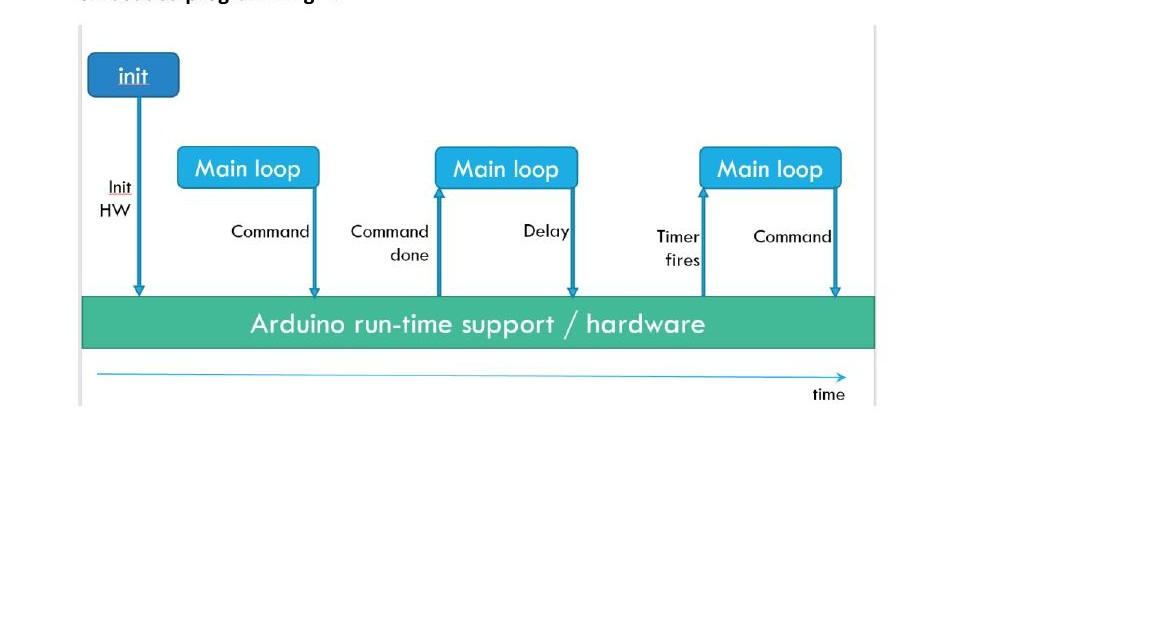
\includegraphics[keepaspectratio]{images/exam-chessa-embedded-arduino.jpg}}
\caption{Modello di esecuzione Arduino: init → loop() ripetuto. I
comandi attivano l'hardware; delay() aspetta; il timer fires avvia la
ripetizione.}
\end{figure}

Lo schema mostra il \textbf{modello di programmazione Arduino}, basato
su un singolo thread di esecuzione:

\begin{enumerate}
\def\labelenumi{\arabic{enumi}.}
\tightlist
\item
  \textbf{init}: la funzione \texttt{setup()} viene eseguita una sola
  volta all'avvio. Inizializza l'hardware, configura i pin, prepara le
  comunicazioni seriali.
\item
  \textbf{Main loop}: la funzione \texttt{loop()} viene invocata
  ripetutamente all'infinito dal runtime Arduino.
\item
  \textbf{Command}: dentro \texttt{loop()}, il codice interagisce con
  l'hardware tramite comandi sincroni (es. \texttt{analogRead()},
  \texttt{Serial.println()}).
\item
  \textbf{Delay}: \texttt{delay(ms)} blocca l'esecuzione per il tempo
  specificato (busy waiting o sleep), poi il timer fires riavvia il
  loop.
\end{enumerate}

Il modello è semplice ma \textbf{bloccante}: durante \texttt{delay()} il
processore non può fare altro. Gli interrupt possono intervenire anche
durante il delay (come mostrato nel codice Arduino interrupt), ma il
thread principale rimane sospeso.

\textbf{Differenza con TinyOS}: nel modello Arduino tutto avviene
sequenzialmente in un unico thread. In TinyOS (modello event-driven) il
sistema reagisce ad eventi: non c'è un loop esplicito, ma handler che si
concatenano tramite eventi hardware.

\begin{calloutnote}{Riferimento}

{[}{[}Lezione 23 - Embedded Programming e Arduino{]}{]}

\end{calloutnote}

\begin{center}\rule{0.5\linewidth}{0.5pt}\end{center}

\section{Embedded Programming - II (Modello
TinyOS/Event-Driven)}\label{embedded-programming---ii-modello-tinyosevent-driven}

\begin{figure}
\centering
\pandocbounded{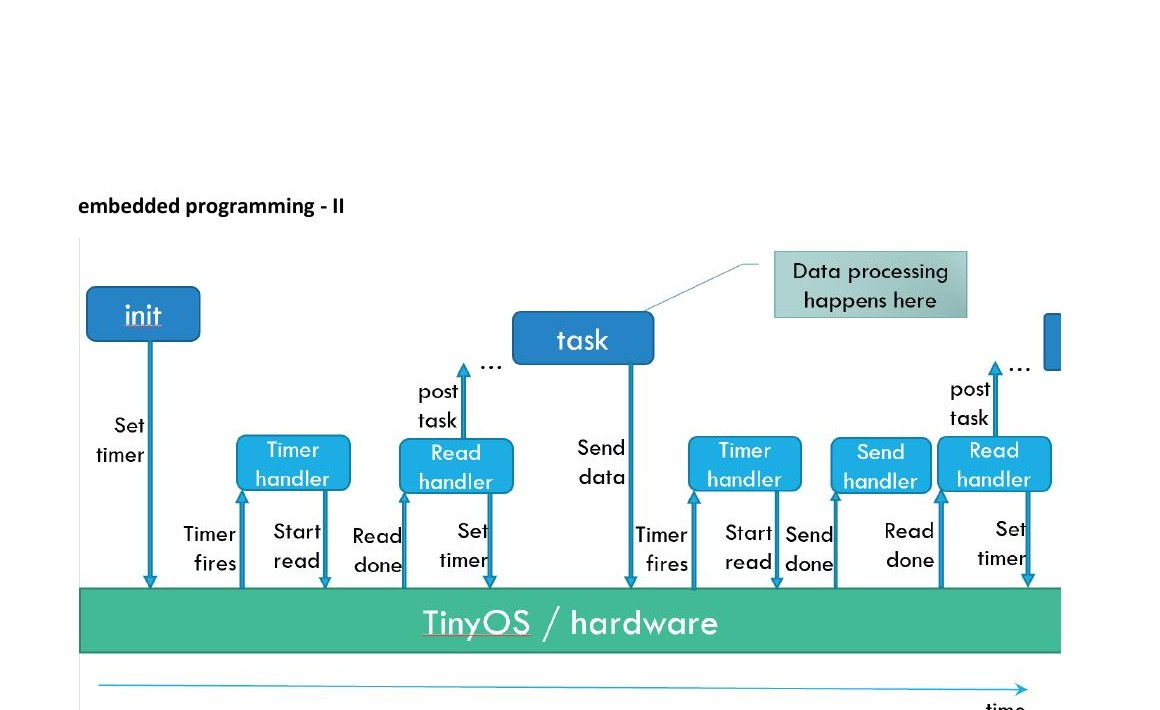
\includegraphics[keepaspectratio]{images/exam-chessa-embedded-tinyos.jpg}}
\caption{Modello di esecuzione TinyOS: catena di eventi (Timer → Read →
task → Send) senza loop bloccante. Il data processing avviene nel task
asincrono.}
\end{figure}

TinyOS usa un modello \textbf{event-driven} con componenti e interfacce.
Non esiste un loop bloccante: il sistema è guidato dagli eventi
hardware. Lo schema mostra una catena tipica:

\begin{enumerate}
\def\labelenumi{\arabic{enumi}.}
\tightlist
\item
  \textbf{init}: configura timer e hardware.
\item
  \textbf{Timer handler} (evento): scatta quando il timer fires → avvia
  una lettura dal sensore (\texttt{Start\ read}).
\item
  \textbf{Read handler} (evento): scatta quando la lettura è completata
  (\texttt{Read\ done}) → posta un task per il processing.
\item
  \textbf{task}: elabora i dati (\emph{Data processing happens here}) →
  avvia la trasmissione radio.
\item
  \textbf{Send handler} (evento): scatta quando la trasmissione è
  completa → riconfigura il timer per il prossimo ciclo.
\end{enumerate}

\textbf{Vantaggi del modello event-driven}: - Nessun busy waiting: il
processore dorme tra un evento e l'altro. - Nessuno stack multiplo: un
unico stack (run-to-completion semantics). - Efficienza energetica: il
MCU è attivo solo durante gli handler.

\textbf{Confronto con Arduino}: Arduino è più semplice da programmare
(loop sequenziale), ma meno efficiente in termini energetici. TinyOS è
ottimale per nodi a basso consumo (mica motes, TMote Sky) dove ogni
microsecondo di sleep conta.

\begin{calloutnote}{Riferimento}

{[}{[}Lezione 23 - Embedded Programming e Arduino{]}{]}

\end{calloutnote}

\begin{center}\rule{0.5\linewidth}{0.5pt}\end{center}

\section{Arduino - Interrupt}\label{arduino---interrupt}

\begin{figure}
\centering
\pandocbounded{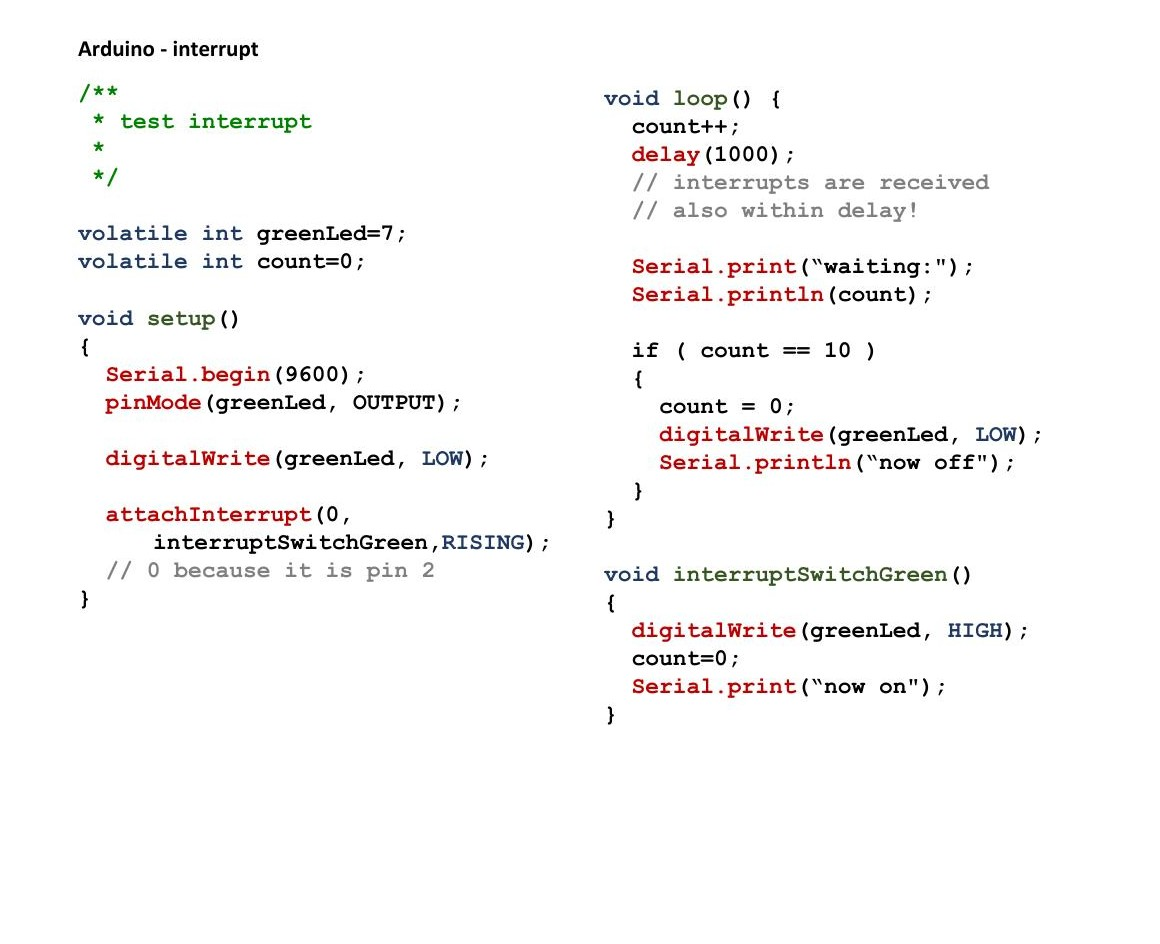
\includegraphics[keepaspectratio]{images/exam-chessa-arduino-interrupt.jpg}}
\caption{Esempio di programmazione con interrupt su Arduino:
attachInterrupt() collega il pin 2 a interruptSwitchGreen(); count viene
resettato e il LED acceso all'interrupt.}
\end{figure}

Il codice mostra il meccanismo degli \textbf{interrupt hardware} su
Arduino:

\begin{Shaded}
\begin{Highlighting}[]
\AttributeTok{volatile} \DataTypeTok{int}\NormalTok{ count }\OperatorTok{=} \DecValTok{0}\OperatorTok{;}
\NormalTok{attachInterrupt}\OperatorTok{(}\DecValTok{0}\OperatorTok{,}\NormalTok{ interruptSwitchGreen}\OperatorTok{,}\NormalTok{ RISING}\OperatorTok{);}
\end{Highlighting}
\end{Shaded}

\texttt{attachInterrupt(0,\ handler,\ RISING)} collega il pin 2
(interrupt 0 su Arduino Uno) alla funzione
\texttt{interruptSwitchGreen}, eseguita automaticamente sul fronte di
salita del segnale.

\textbf{Punti chiave}: - La variabile \texttt{count} è dichiarata
\texttt{volatile}: indica al compilatore di non ottimizzarla in
registro, perché può essere modificata da handler fuori dal flusso
normale. - Gli interrupt sono ricevuti \textbf{anche durante
\texttt{delay()}} (come nota il commento): il delay non disabilita gli
interrupt, quindi l'handler può intervenire in qualsiasi momento. -
L'interrupt resetta \texttt{count=0} e accende il LED verde; il loop
principale incrementa \texttt{count}, aspetta 1 secondo, e gestisce il
timeout a 10.

\textbf{Utilizzo tipico negli embedded IoT}: gli interrupt sono usati
per ricevere dati dal sensore (read done), notificare la fine di una
trasmissione radio, o rispondere a eventi fisici (pressione di un
pulsante) senza polling continuo, risparmiando energia.

\begin{calloutnote}{Riferimento}

{[}{[}Lezione 23 - Embedded Programming e Arduino{]}{]}

\end{calloutnote}

\begin{center}\rule{0.5\linewidth}{0.5pt}\end{center}

\section{SMAC (Sensor-MAC)}\label{smac-sensor-mac}

\begin{figure}
\centering
\pandocbounded{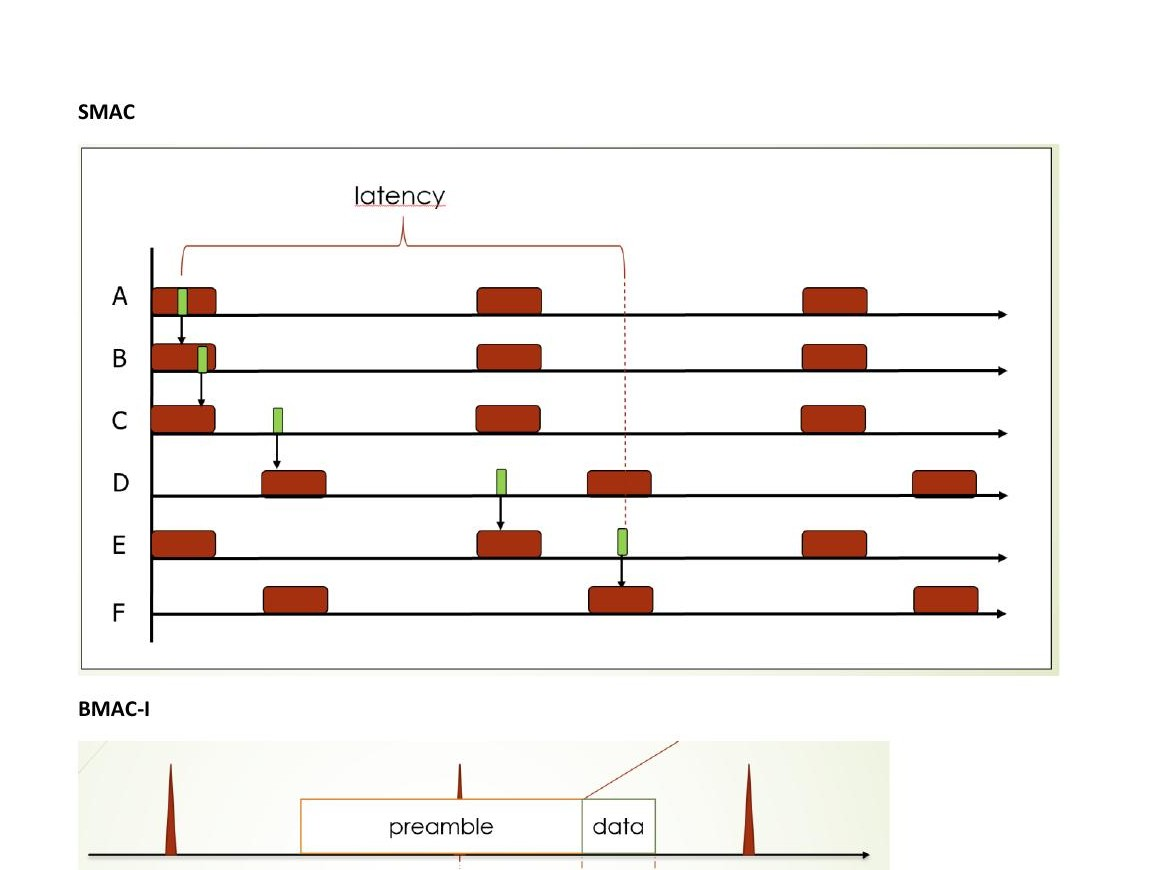
\includegraphics[keepaspectratio]{images/exam-chessa-smac.jpg}}
\caption{S-MAC: i nodi A--F hanno schedule sincronizzati (verde =
listen, rosso = active/TX). La latenza multi-hop si accumula: il
pacchetto da A deve aspettare i periodi di ascolto di ogni hop
successivo.}
\end{figure}

\textbf{S-MAC} (\emph{Sensor MAC}) è un protocollo MAC per WSN che
riduce il consumo energetico tramite \textbf{sincronizzazione locale}:
nodi vicini si accordano su un periodo di ascolto comune (listen period)
e dormono nel resto del tempo.

\textbf{Meccanismo}: 1. Ogni nodo trasmette periodicamente un pacchetto
\textbf{SYNC} che annuncia il proprio schedule (quando si sveglierà). 2.
I vicini che ricevono il SYNC adottano lo stesso schedule o mantengono
il proprio e memorizzano quello del vicino. 3. Nel \textbf{listen
period}: esecuzione di CSMA/CA con RTS/CTS prima di trasmettere. 4. Nel
\textbf{sleep period}: la radio è spenta.

\textbf{Duty cycle}: definito come
\(DC = t_{listen} / (t_{listen} + t_{sleep})\), tipicamente 10\% in
S-MAC.

\textbf{Problema della latenza multi-hop}: come visibile nello schema,
ogni nodo deve aspettare il periodo di ascolto del nodo successivo. La
latenza totale si accumula: se ogni hop aggiunge un'attesa
\(\approx t_{sleep}\), un percorso di \(n\) hop ha latenza
\(\approx n \cdot (t_{sleep}/2)\) in media.

\textbf{Adaptive duty cycle}: se un nodo riceve un RTS o CTS (anche non
destinato a lui), capisce che c'è traffico nelle vicinanze e mantiene la
radio accesa --- potrebbe essere il prossimo hop e il messaggio arriverà
presto.

\begin{calloutnote}{Riferimento}

{[}{[}Lezione 17 - MAC Protocols{]}{]}

\end{calloutnote}

\begin{center}\rule{0.5\linewidth}{0.5pt}\end{center}

\section{BMAC - I (Struttura del
Protocollo)}\label{bmac---i-struttura-del-protocollo}

\begin{figure}
\centering
\pandocbounded{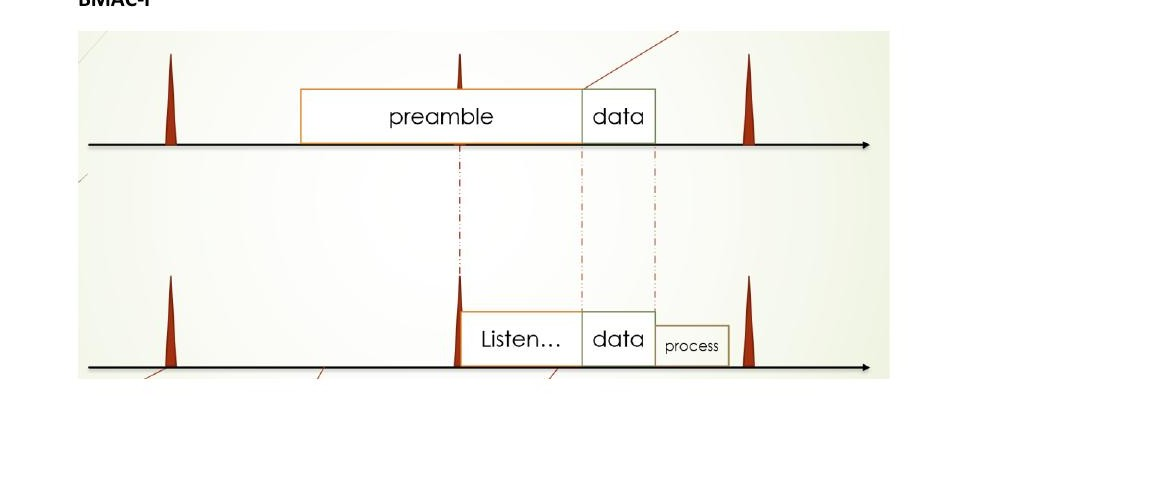
\includegraphics[keepaspectratio]{images/exam-chessa-bmac.jpg}}
\caption{B-MAC: il mittente (in alto) invia un lungo preamble seguito
dai data; il ricevitore (in basso) si sveglia, ascolta, individua il
preamble, rimane sveglio e riceve i data.}
\end{figure}

\textbf{B-MAC} (\emph{Berkeley MAC}) usa un approccio completamente
diverso da S-MAC: \textbf{nessuna sincronizzazione} tra i nodi. Il
principio è il \textbf{preamble sampling} (o Low Power Listening, LPL):

\textbf{Lato ricevitore}: - Si sveglia periodicamente ogni \(t_{check}\)
millisecondi. - Campiona il canale per un breve istante. - Se rileva
attività (preamble), rimane sveglio e riceve il pacchetto dati. -
Altrimenti, si riaddormenta immediatamente.

\textbf{Lato mittente}: - Quando vuole trasmettere, invia un
\textbf{preamble lungo} per una durata \textgreater{} \(t_{check}\). -
Questo garantisce che, qualunque sia il momento in cui il ricevitore si
sveglia per campionare, troverà il preamble ancora in corso. - Dopo il
preamble, invia i dati effettivi.

\textbf{Confronto con S-MAC}: - B-MAC non richiede sincronizzazione →
deployment più semplice. - Il preamble lungo consuma energia extra dal
mittente. - Il ricevitore non spreca energia in lunghi listen period, ma
solo in brevi campionamenti.

\begin{calloutnote}{Riferimento}

{[}{[}Lezione 17 - MAC Protocols{]}{]}

\end{calloutnote}

\begin{center}\rule{0.5\linewidth}{0.5pt}\end{center}

\section{BMAC - II (Trade-off t\_check e Vita del
Trasmettitore)}\label{bmac---ii-trade-off-t_check-e-vita-del-trasmettitore}

\begin{figure}
\centering
\pandocbounded{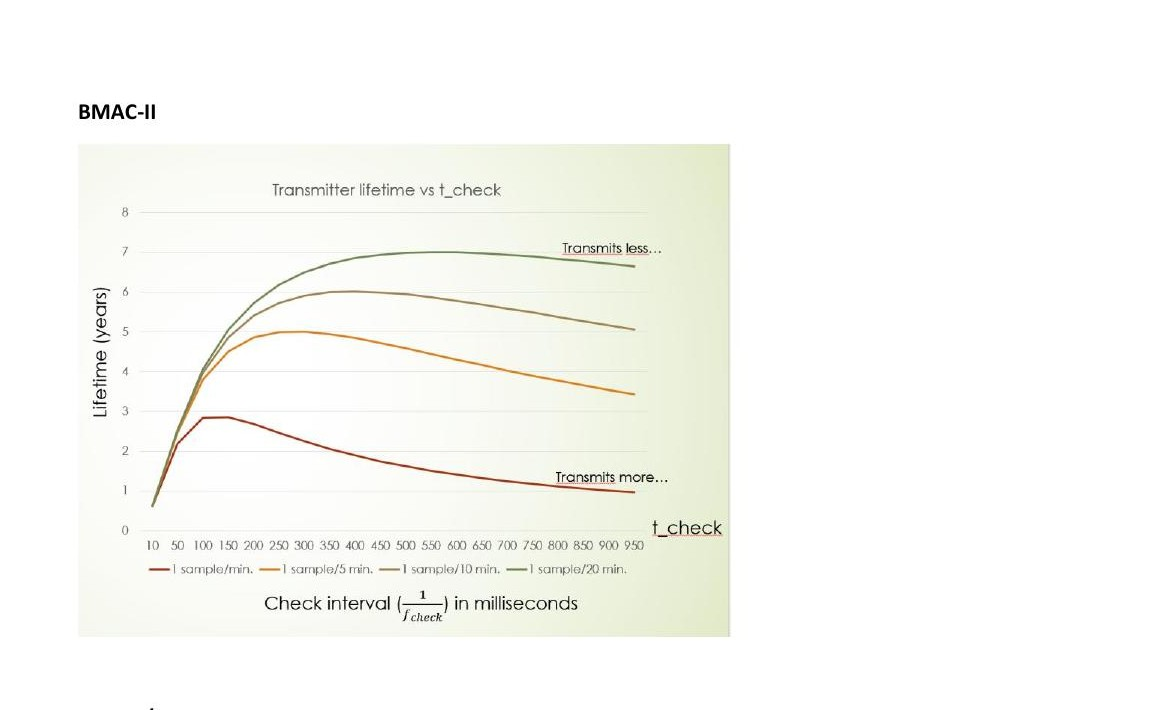
\includegraphics[keepaspectratio]{images/exam-chessa-bmac-graph.jpg}}
\caption{Grafico B-MAC: vita del trasmettitore (anni) vs intervallo di
check t\_check (ms), per diverse frequenze di campionamento (1
sample/min, 1/5 min, 1/10 min, 1/20 min).}
\end{figure}

Il grafico mostra il trade-off fondamentale di B-MAC: come la frequenza
di trasmissione e l'intervallo \(t_{check}\) influenzano la vita della
batteria del \textbf{trasmettitore}.

\textbf{Interpretazione}: - Ogni curva rappresenta una diversa frequenza
di campionamento dati (1 campione/minuto → consumo più alto, 1
campione/20 minuti → consumo più basso). - Al crescere di \(t_{check}\)
(asse x), il preamble deve essere più lungo (per garantire che il
ricevitore lo trovi), quindi il trasmettitore consuma di più per ogni
trasmissione. - Tuttavia, la vita del trasmettitore ha un
\textbf{massimo} per un valore ottimale di \(t_{check}\): troppo breve →
il ricevitore si sveglia spesso ma il preamble è corto (basso overhead);
troppo lungo → preamble lunghissimo, overhead alto. - Per frequenze di
trasmissione più basse (1/20 min), il trasmettitore vive molto più a
lungo (fino a 7+ anni).

\textbf{Conclusione}: il parametro \(t_{check}\) va ottimizzato in base
al profilo di trasmissione dell'applicazione. Non esiste un valore
universalmente ottimale.

\begin{calloutnote}{Riferimento}

{[}{[}Lezione 17 - MAC Protocols{]}{]}

\end{calloutnote}

\begin{center}\rule{0.5\linewidth}{0.5pt}\end{center}

\section{X-MAC / B-MAC (Confronto LPL vs
X-MAC)}\label{x-mac-b-mac-confronto-lpl-vs-x-mac}

\begin{figure}
\centering
\pandocbounded{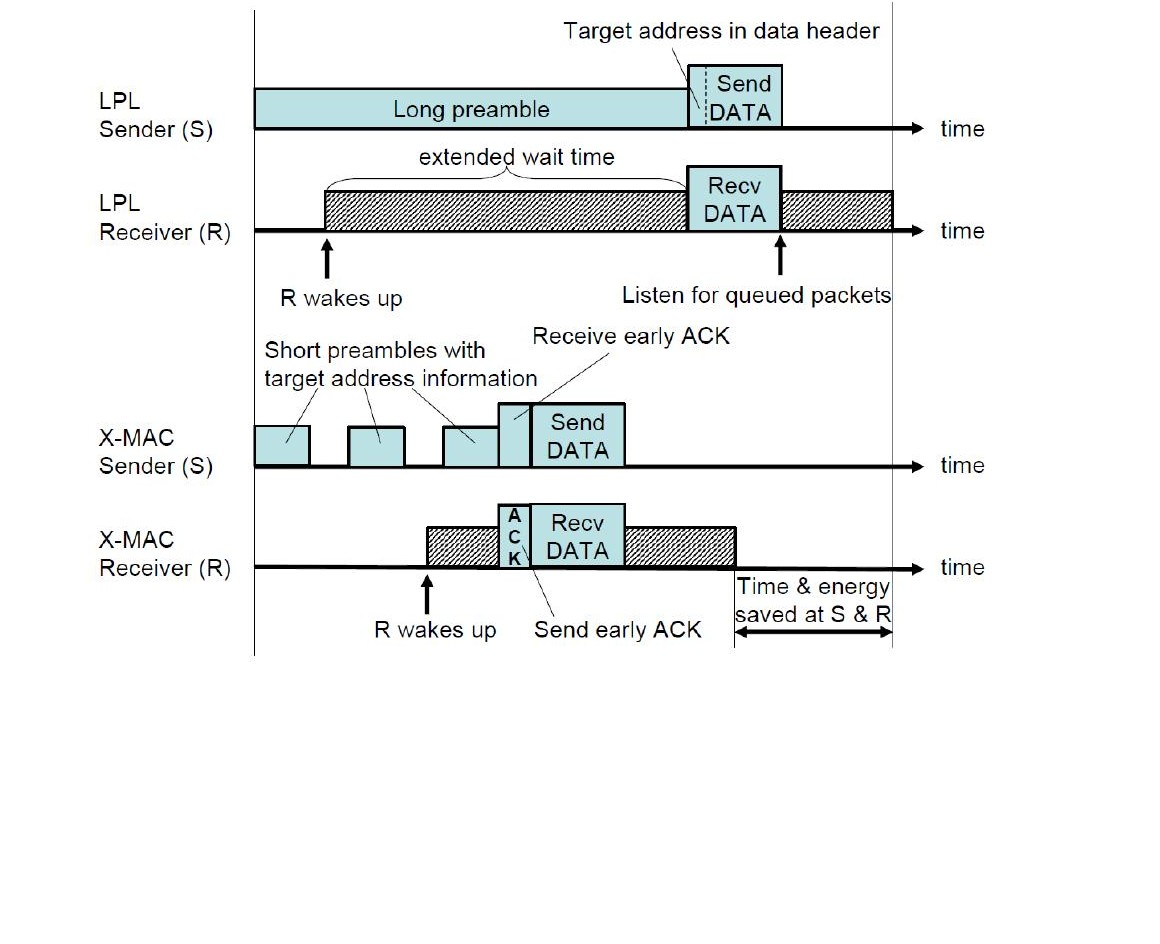
\includegraphics[keepaspectratio]{images/exam-chessa-xmac.jpg}}
\caption{Confronto LPL (B-MAC, righe superiori) e X-MAC (righe
inferiori): X-MAC usa preamble corti con indirizzo target; il ricevitore
invia early ACK; mittente e ricevitore risparmiano tempo ed energia.}
\end{figure}

\textbf{X-MAC} migliora B-MAC risolvendo lo spreco energetico del long
preamble con i \textbf{short preamble strobes} con target address:

\textbf{LPL (B-MAC)}: - Mittente: invia un unico preamble lungo
\textgreater{} \(t_{check}\), poi i dati. - Ricevitore: si sveglia,
trova il preamble, rimane sveglio per tutta la durata del preamble +
dati. - \textbf{Problema}: anche i nodi non destinatari che si svegliano
durante il preamble restano svegli inutilmente (overhearing).

\textbf{X-MAC}: - Mittente: invia una sequenza di \textbf{short
preambles} contenenti ciascuno l'indirizzo del destinatario target. -
Ricevitore target: si sveglia, legge il proprio indirizzo nel preamble,
invia immediatamente un \textbf{early ACK}. - Mittente: riceve l'ACK →
interrompe la sequenza di preamble → trasmette i dati direttamente. -
\textbf{Risparmio}: il mittente non deve completare tutta la sequenza di
preamble; il ricevitore non aspetta un preamble lungo. -
\textbf{Risparmio per i non-destinatari}: vedono il proprio indirizzo
assente nel preamble → si riaddormentano subito.

Il risultato è un risparmio sia per il mittente (preamble più corto in
media) sia per il ricevitore (less idle listening), indicato nello
schema come ``Time \& energy saved at S \& R''.

\begin{calloutnote}{Riferimento}

{[}{[}Lezione 17 - MAC Protocols{]}{]}

\end{calloutnote}

\begin{center}\rule{0.5\linewidth}{0.5pt}\end{center}

\section{IEEE 802.15.4 - I (Struttura del
Superframe)}\label{ieee-802.15.4---i-struttura-del-superframe}

\begin{figure}
\centering
\pandocbounded{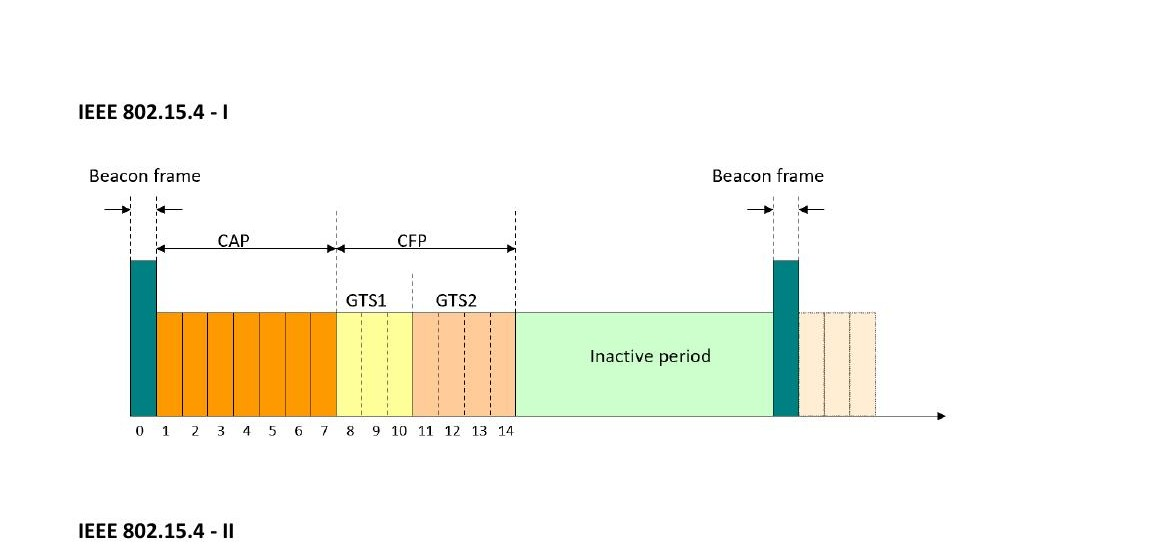
\includegraphics[keepaspectratio]{images/exam-chessa-ieee802154-superframe.jpg}}
\caption{Struttura del superframe IEEE 802.15.4: Beacon frame → CAP
(Contention Access Period, slot 0--6) → CFP (Contention Free Period,
GTS1 e GTS2, slot 7--11) → Inactive period (slot 12--14) → prossimo
Beacon.}
\end{figure}

IEEE 802.15.4 definisce una struttura temporale chiamata
\textbf{superframe} per organizzare l'accesso al canale in reti
beacon-enabled:

\textbf{Beacon frame}: il coordinatore trasmette periodicamente un
beacon che annuncia l'inizio del superframe, contiene i parametri della
rete e la lista dei dispositivi con dati pendenti.

\textbf{CAP (Contention Access Period)}: periodo di accesso conteso
tramite \textbf{CSMA/CA slottato}. Tutti i dispositivi competono per
l'accesso al canale. Usato per traffico non deterministico (dati
aperiodici).

\textbf{CFP (Contention Free Period)}: suddiviso in \textbf{GTS
(Guaranteed Time Slots)}, assegnati dal coordinatore a specifici
dispositivi per comunicazioni deterministiche a bassa latenza. Fino a 7
GTS per superframe. Usato per applicazioni real-time che richiedono
garanzie temporali.

\textbf{Inactive period}: tutti i dispositivi (incluso il coordinatore)
possono dormire per risparmiare energia. La durata del periodo inattivo
determina il duty cycle della rete.

La durata del superframe è configurabile e determina il duty cycle: un
inactive period lungo → basso duty cycle → lunga vita della batteria →
latenza più alta.

\begin{calloutnote}{Riferimento}

{[}{[}Lezione 18 - The IEEE 802.15.4 Standard{]}{]}

\end{calloutnote}

\begin{center}\rule{0.5\linewidth}{0.5pt}\end{center}

\section{IEEE 802.15.4 - II (Indirect Data
Transfer)}\label{ieee-802.15.4---ii-indirect-data-transfer}

\begin{figure}
\centering
\pandocbounded{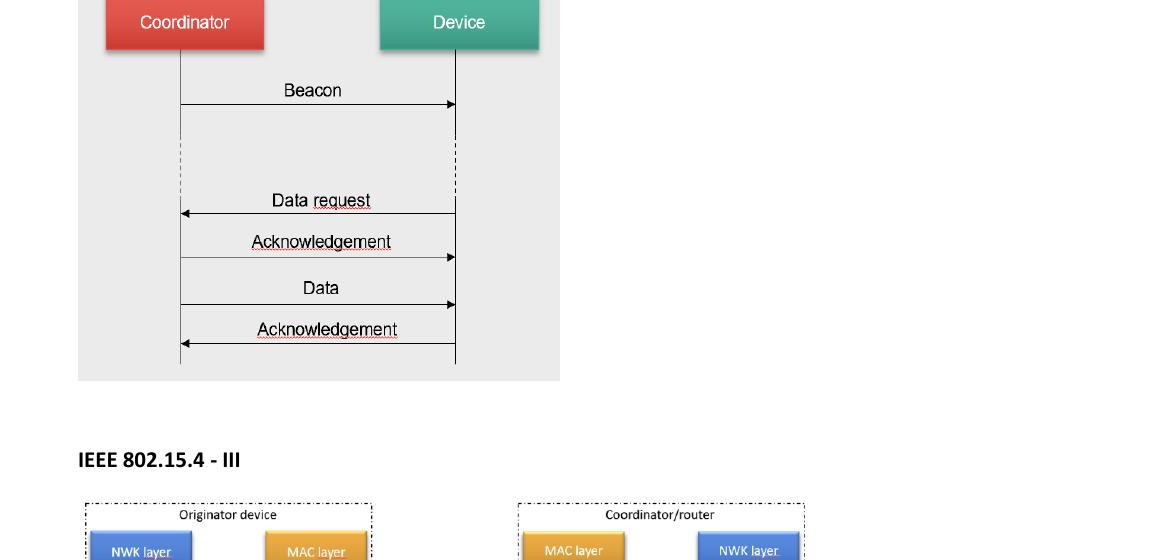
\includegraphics[keepaspectratio]{images/exam-chessa-ieee802154-indirect.jpg}}
\caption{Trasferimento dati indiretto in IEEE 802.15.4: il dispositivo
si sveglia al beacon, invia una Data request al coordinatore, riceve ACK
e poi i dati.}
\end{figure}

Il trasferimento \textbf{indiretto} è usato quando il destinatario è un
dispositivo che dorme la maggior parte del tempo (RFD, end-device). Il
coordinatore non può trasmettere dati in modo asincrono perché il
dispositivo potrebbe essere in sleep.

\textbf{Sequenza}: 1. Il \textbf{coordinatore} trasmette un
\textbf{Beacon} che include (nella lista \emph{pending addresses})
l'indirizzo dei dispositivi per cui ha dati in coda. 2. Il
\textbf{dispositivo} si sveglia al beacon, legge la lista, se vede il
proprio indirizzo invia una \textbf{Data request} al coordinatore. 3. Il
\textbf{coordinatore} risponde con un \textbf{Acknowledgement}
immediato. 4. Il \textbf{coordinatore} trasmette i \textbf{dati}
accodati. 5. Il \textbf{dispositivo} risponde con un
\textbf{Acknowledgement}.

Il device può poi tornare in sleep. Il vantaggio è che il dispositivo
non deve rimanere sveglio ad aspettare dati: si sveglia solo al beacon
(duty cycle controllato), controlla se ci sono dati per lui, li recupera
e dorme di nuovo.

\begin{calloutnote}{Riferimento}

{[}{[}Lezione 18 - The IEEE 802.15.4 Standard{]}{]}

\end{calloutnote}

\begin{center}\rule{0.5\linewidth}{0.5pt}\end{center}

\section{IEEE 802.15.4 - III (Protocollo di
Associazione)}\label{ieee-802.15.4---iii-protocollo-di-associazione}

\begin{figure}
\centering
\pandocbounded{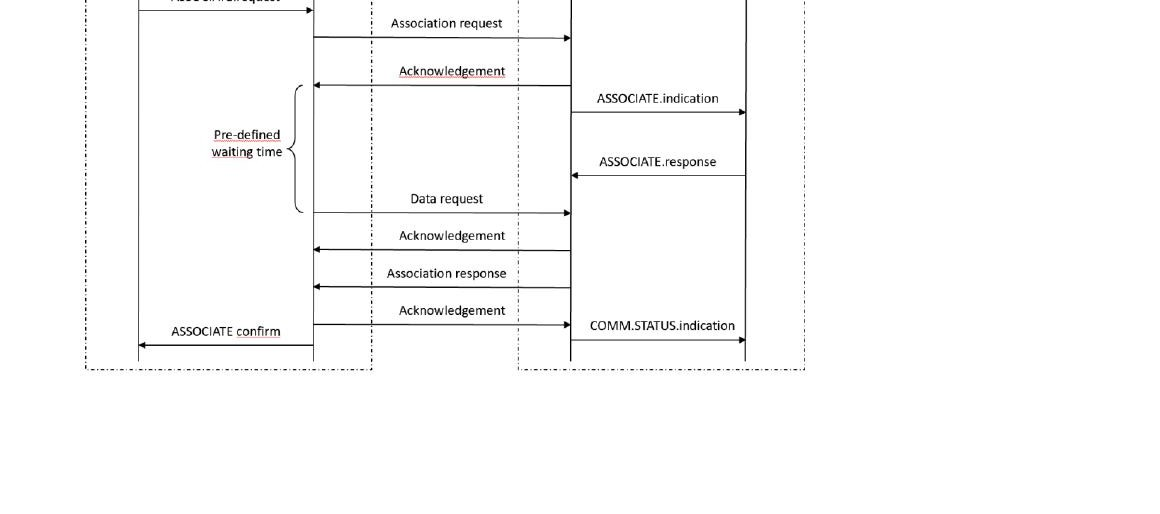
\includegraphics[keepaspectratio]{images/exam-chessa-ieee802154-association.jpg}}
\caption{Protocollo di associazione IEEE 802.15.4: sequenza di messaggi
tra NWK e MAC layer del dispositivo (sinistra) e del coordinatore/router
(destra).}
\end{figure}

Lo schema mostra il protocollo di \textbf{associazione} visto a livello
di primitives NWK-MAC. È il meccanismo con cui un dispositivo entra
nella rete:

\begin{enumerate}
\def\labelenumi{\arabic{enumi}.}
\tightlist
\item
  Il NWK del dispositivo emette \texttt{ASSOCIATE.request} al proprio
  MAC layer.
\item
  Il MAC invia un \textbf{Association request} frame al coordinatore.
\item
  Il coordinatore MAC risponde con \textbf{Acknowledgement} immediato.
\item
  Il coordinatore NWK riceve \texttt{ASSOCIATE.indication} e prepara la
  risposta con \texttt{ASSOCIATE.response}.
\item
  Il dispositivo aspetta un \textbf{pre-defined waiting time} (il
  coordinatore deve elaborare la richiesta e decidere se accettarla).
\item
  Il dispositivo MAC invia una \textbf{Data request} per recuperare la
  risposta del coordinatore.
\item
  Il coordinatore MAC risponde con \textbf{Acknowledgement} +
  \textbf{Association response} (contenente l'indirizzo a 16 bit
  assegnato).
\item
  Il dispositivo MAC invia \textbf{Acknowledgement} finale.
\item
  Il dispositivo NWK riceve \texttt{ASSOCIATE\ confirm} con l'indirizzo
  assegnato.
\item
  Il coordinatore NWK riceve \texttt{COMM.STATUS.indication}.
\end{enumerate}

Questo è il meccanismo di basso livello che corrisponde a
\texttt{ASSOCIATE.request}/\texttt{ASSOCIATE.confirm} nelle primitive
ZigBee viste nello schema ZigBee-I.

\begin{calloutnote}{Riferimento}

{[}{[}Lezione 18 - The IEEE 802.15.4 Standard{]}{]}

\end{calloutnote}

\begin{center}\rule{0.5\linewidth}{0.5pt}\end{center}

\section{Energy Harvesting --- Domande
Generali}\label{energy-harvesting-domande-generali}

\begin{calloutquestion}{Domande del PDF}

\begin{itemize}
\tightlist
\item
  Explain the difference between an harvest-use and an harvest-store-use
  architecture
\item
  Explain the classification of sources in terms of controllability and
  predictability
\item
  Explain the concept of energy neutrality
\end{itemize}

\end{calloutquestion}

\subsection{Harvest-Use vs
Harvest-Store-Use}\label{harvest-use-vs-harvest-store-use}

\textbf{Harvest-Use}: l'energia è raccolta e consumata istantaneamente.
Non esiste un buffer. Il dispositivo funziona solo se
\(P_s(t) \geq P_c(t)\) (potenza sorgente ≥ potenza consumata). Se la
sorgente produce meno del necessario il dispositivo si spegne; se
produce di più l'eccesso va perduto. Esempi: mulini ad acqua, tag RFID
passivi.

\textbf{Harvest-Store-Use}: un buffer energetico (batteria ricaricabile
o supercapacitore) disaccoppia temporalmente produzione e consumo.
L'energia in eccesso (\(P_s > P_c\)) viene accumulata nel buffer;
l'energia in difetto (\(P_c > P_s\)) viene prelevata dal buffer. Un
buffer ideale ha capacità infinita ed efficienza \(\eta = 1\). Un buffer
reale ha capacità massima \(B_{max}\), efficienza \(\eta < 1\), e una
potenza di leakage \(P_{leak}\).

\subsection{Classificazione delle
Sorgenti}\label{classificazione-delle-sorgenti}

Le sorgenti si classificano su due assi:

\textbf{Controllabilità}: - \emph{Completamente controllabile}: energia
disponibile su richiesta (torcia shake-to-power, sorgenti RF dedicate).
- \emph{Parzialmente controllabile}: influenzabile ma non deterministica
(RFID in ambiente RF non uniforme). - \emph{Non controllabile}: raccolta
solo quando disponibile (sole, vento, calore ambientale).

\textbf{Prevedibilità} (per le sorgenti non controllabili): -
\emph{Prevedibile}: esistono modelli affidabili (sole: ciclo
giorno/notte + stagioni + meteo). - \emph{Non prevedibile}: nessun
modello affidabile (vibrazioni da terremoti).

\subsection{Concetto di Energy
Neutrality}\label{concetto-di-energy-neutrality}

Un dispositivo è \textbf{energy neutral} se, in qualsiasi intervallo di
tempo, l'energia consumata non supera l'energia raccolta (più la carica
iniziale del buffer):

\[\int_0^T P_c(t)\,dt \leq \int_0^T P_s(t)\,dt + B_0 \qquad \forall T\]

Il raggiungimento dell'energy neutrality richiede di adattare il carico
in base alla disponibilità energetica prevista --- obiettivo del
problema di Kansal.

\begin{calloutnote}{Riferimento}

{[}{[}Lezione 24 - Energy Harvesting IoT{]}{]}

\end{calloutnote}

\begin{center}\rule{0.5\linewidth}{0.5pt}\end{center}

\section{Energy Harvesting - I (Grafico Ps vs
Pc)}\label{energy-harvesting---i-grafico-ps-vs-pc}

\begin{figure}
\centering
\pandocbounded{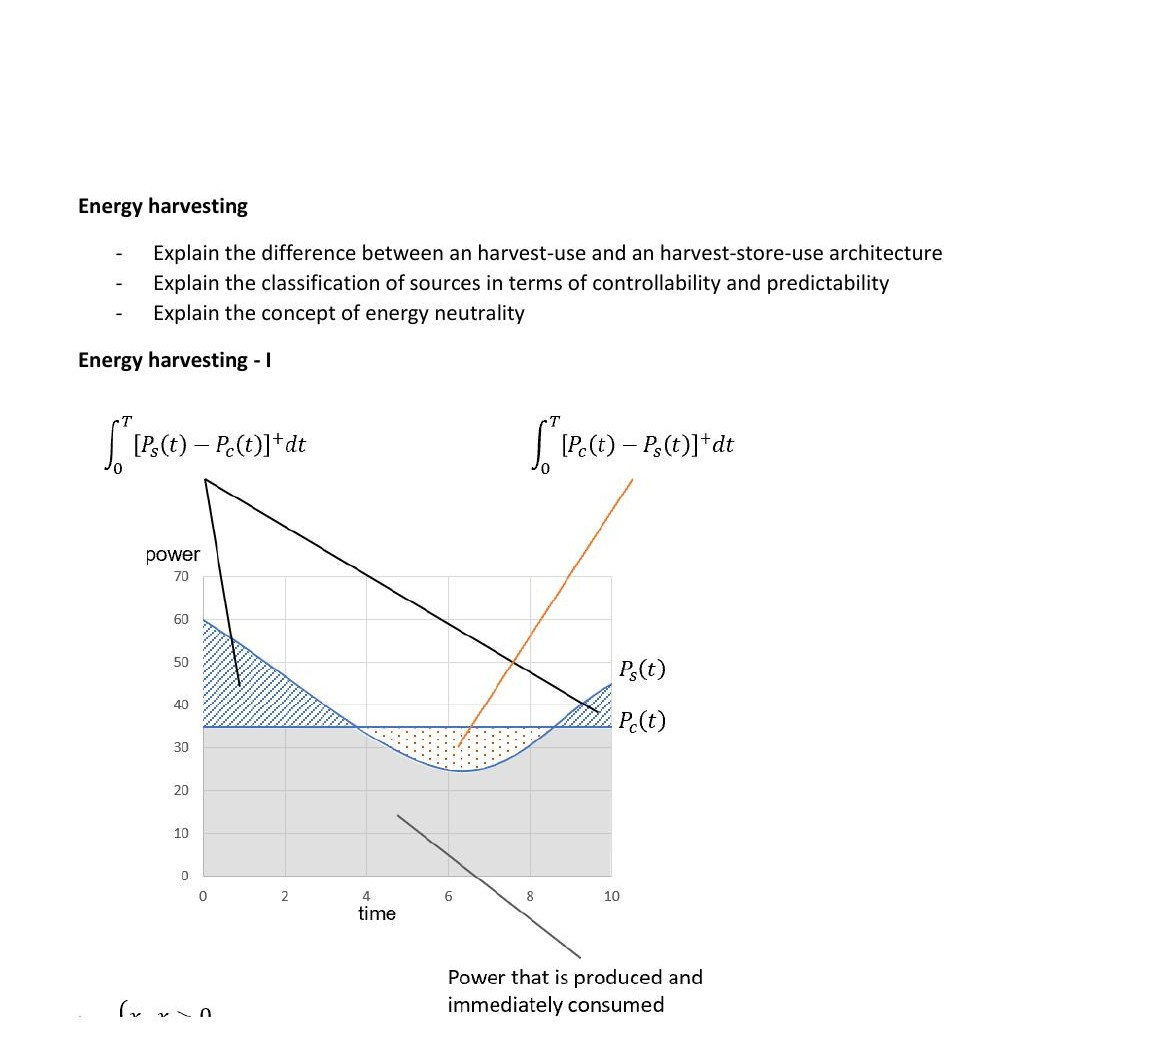
\includegraphics[keepaspectratio]{images/exam-chessa-energy-neutrality-graph.jpg}}
\caption{Grafico potenza/tempo: l'area tratteggiata in blu (Ps
\textgreater{} Pc) è l'energia raccolta e accumulata nel buffer; l'area
punteggiata (Pc \textgreater{} Ps) è l'energia prelevata dal buffer. La
retta arancione mostra l'energia immediatamente consumata (Pc=Ps).}
\end{figure}

Il grafico mostra due curve di potenza in funzione del tempo: -
\(P_s(t)\): potenza prodotta dall'energy harvester (curva decrescente).
- \(P_c(t)\): potenza consumata dal dispositivo (curva a forma di U).

Le due aree rappresentano:

\[\int_0^T [P_s(t) - P_c(t)]^+ dt\]

Area in blu (Ps \textgreater{} Pc, da t≈0 a t≈4): energia prodotta in
eccesso → accumulata nel buffer. Il buffer si carica.

\[\int_0^T [P_c(t) - P_s(t)]^+ dt\]

Area punteggiata (Pc \textgreater{} Ps, da t≈4 a t≈8): il consumo supera
la produzione → energia prelevata dal buffer. Il buffer si scarica.

La retta arancione indica la zona in cui \(P_s = P_c\): energia prodotta
e immediatamente consumata, senza passare dal buffer.

Il sistema è energy neutral se la prima integrale ≥ seconda integrale su
tutto l'orizzonte temporale considerato.

\begin{calloutnote}{Riferimento}

{[}{[}Lezione 24 - Energy Harvesting IoT{]}{]}

\end{calloutnote}

\begin{center}\rule{0.5\linewidth}{0.5pt}\end{center}

\section{Energy Harvesting -- II (Stima Stato di
Carica)}\label{energy-harvesting-ii-stima-stato-di-carica}

\begin{figure}
\centering
\pandocbounded{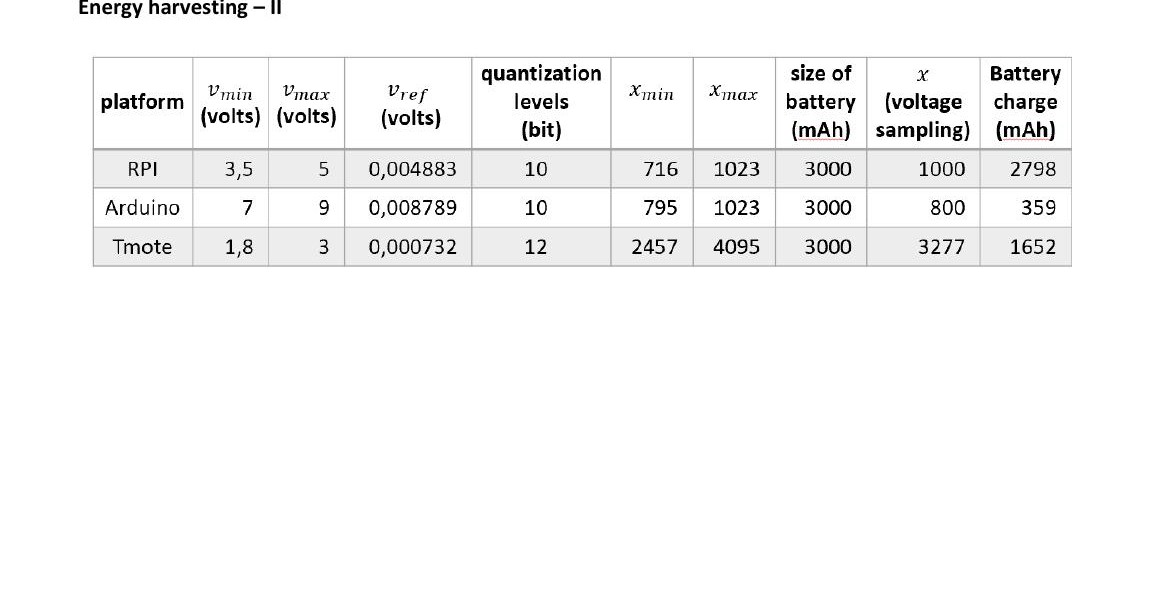
\includegraphics[keepaspectratio]{images/exam-chessa-energy-harvesting-table.jpg}}
\caption{Tabella con parametri di batteria per tre piattaforme (RPI,
Arduino, Tmote): tensioni min/max/ref, livelli di quantizzazione,
xmin/xmax e stima Battery charge.}
\end{figure}

La tabella mostra come misurare lo \textbf{stato di carica} (SoC) di una
batteria attraverso la sua tensione terminale, per tre piattaforme
hardware.

Le colonne chiave: - \(v_{min}\), \(v_{max}\): range operativo della
batteria (es. Arduino: 7--9 V). - \(v_{ref}\): risoluzione della
quantizzazione ADC (es. Arduino: 0.008789 V per LSB). -
\textbf{quantization levels (bit)}: risoluzione dell'ADC (10 o 12 bit).
- \(x_{min}\), \(x_{max}\): valori ADC corrispondenti a \(v_{min}\) e
\(v_{max}\). - \textbf{Battery charge (mAh)}: capacità totale della
batteria stimata.

L'idea è che la tensione ai terminali di una batteria è approssimabile
come monotona rispetto alla carica residua. Campionando la tensione
tramite ADC e mappando il valore digitale \(x\) nell'intervallo
\([x_{min}, x_{max}]\), si ottiene una stima lineare della carica
rimanente:

\[\text{SoC} \approx \frac{x - x_{min}}{x_{max} - x_{min}} \times B_{cap}\]

Questa stima è utile per il task scheduler: sa quanta energia ha
disponibile e può pianificare i task di conseguenza (approccio Kansal).

\begin{calloutnote}{Riferimento}

{[}{[}Lezione 24 - Energy Harvesting IoT{]}{]}

\end{calloutnote}

\begin{center}\rule{0.5\linewidth}{0.5pt}\end{center}

\section{Energy Harvesting -- III (Approccio Kansal all'Energy
Neutrality)}\label{energy-harvesting-iii-approccio-kansal-allenergy-neutrality}

\begin{figure}
\centering
\pandocbounded{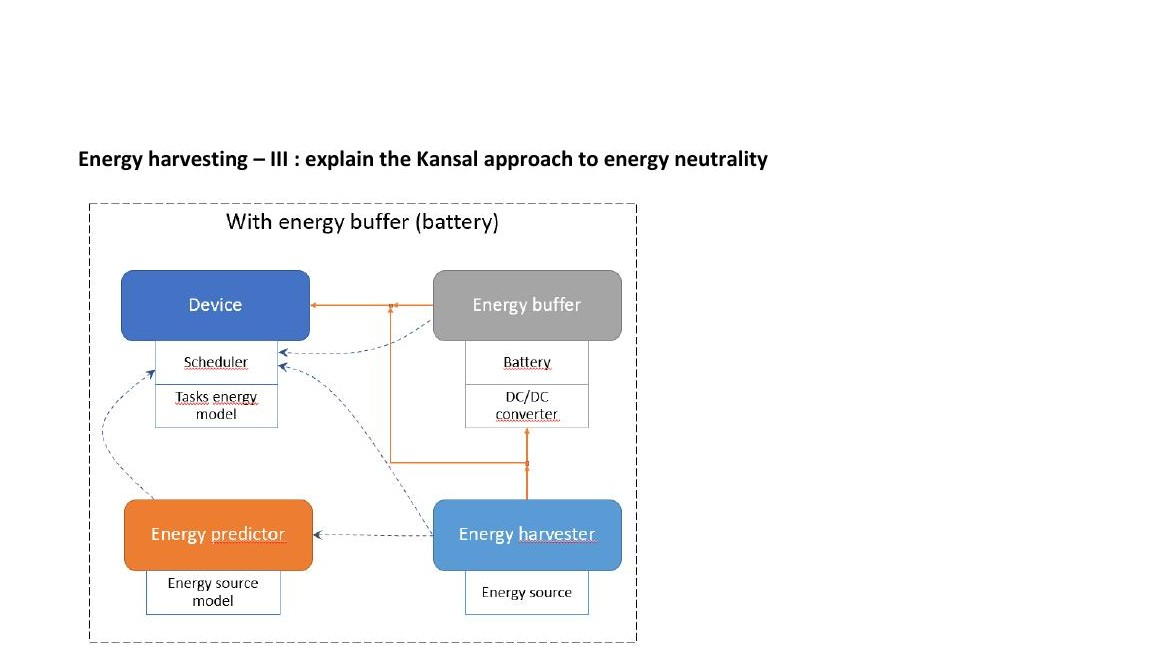
\includegraphics[keepaspectratio]{images/exam-chessa-kansal-system.jpg}}
\caption{Sistema Kansal: il Device (con Scheduler e Tasks energy model)
è alimentato dall'Energy buffer (Battery + DC/DC converter), rifornito
dall'Energy harvester. L'Energy predictor stima la disponibilità futura
e informa lo Scheduler.}
\end{figure}

L'approccio di \textbf{Kansal} all'energy neutrality mira a massimizzare
le prestazioni del dispositivo garantendo al contempo che la batteria
non si scarichi mai completamente (energy neutral operation).

Il sistema è composto da:

\begin{itemize}
\tightlist
\item
  \textbf{Energy harvester}: raccoglie energia dalla sorgente (es.
  pannello solare).
\item
  \textbf{Energy buffer (Battery + DC/DC converter)}: accumula l'energia
  raccolta e la cede al dispositivo quando necessario.
\item
  \textbf{Energy predictor} (con Energy source model): stima la quantità
  di energia che sarà disponibile nel futuro (ad es. usando previsioni
  meteo per un pannello solare).
\item
  \textbf{Device} con \textbf{Scheduler} (e Tasks energy model):
  pianifica quali task eseguire e a quale frequenza, basandosi sia sullo
  stato attuale della batteria sia sulla predizione energetica futura.
\end{itemize}

\textbf{Idea centrale}: adattare il carico (\(P_c\)) alla disponibilità
energetica prevista. Se le previsioni indicano un giorno soleggiato → il
dispositivo può aumentare la frequenza di campionamento. Se le
previsioni indicano bassa produzione → il dispositivo riduce l'attività.

\textbf{Condizione di energy neutrality di Kansal}:

\[B_T = B_0 + \eta \int_0^T [P_s - P_c]^+ dt - \int_0^T [P_c - P_s]^+ dt \geq B_{min} \quad \forall T\]

Il Kansal problem è quindi un problema di ottimizzazione: massimizzare
le prestazioni (es. frequenza di campionamento) soggetto al vincolo di
energy neutrality.

\begin{calloutnote}{Riferimento}

{[}{[}Lezione 28 - Kansal Problem e Energy Neutrality{]}{]}

\end{calloutnote}

\begin{center}\rule{0.5\linewidth}{0.5pt}\end{center}

\section{Energy Harvesting -- IV (Task Model per l'Energy
Neutrality)}\label{energy-harvesting-iv-task-model-per-lenergy-neutrality}

\begin{figure}
\centering
\pandocbounded{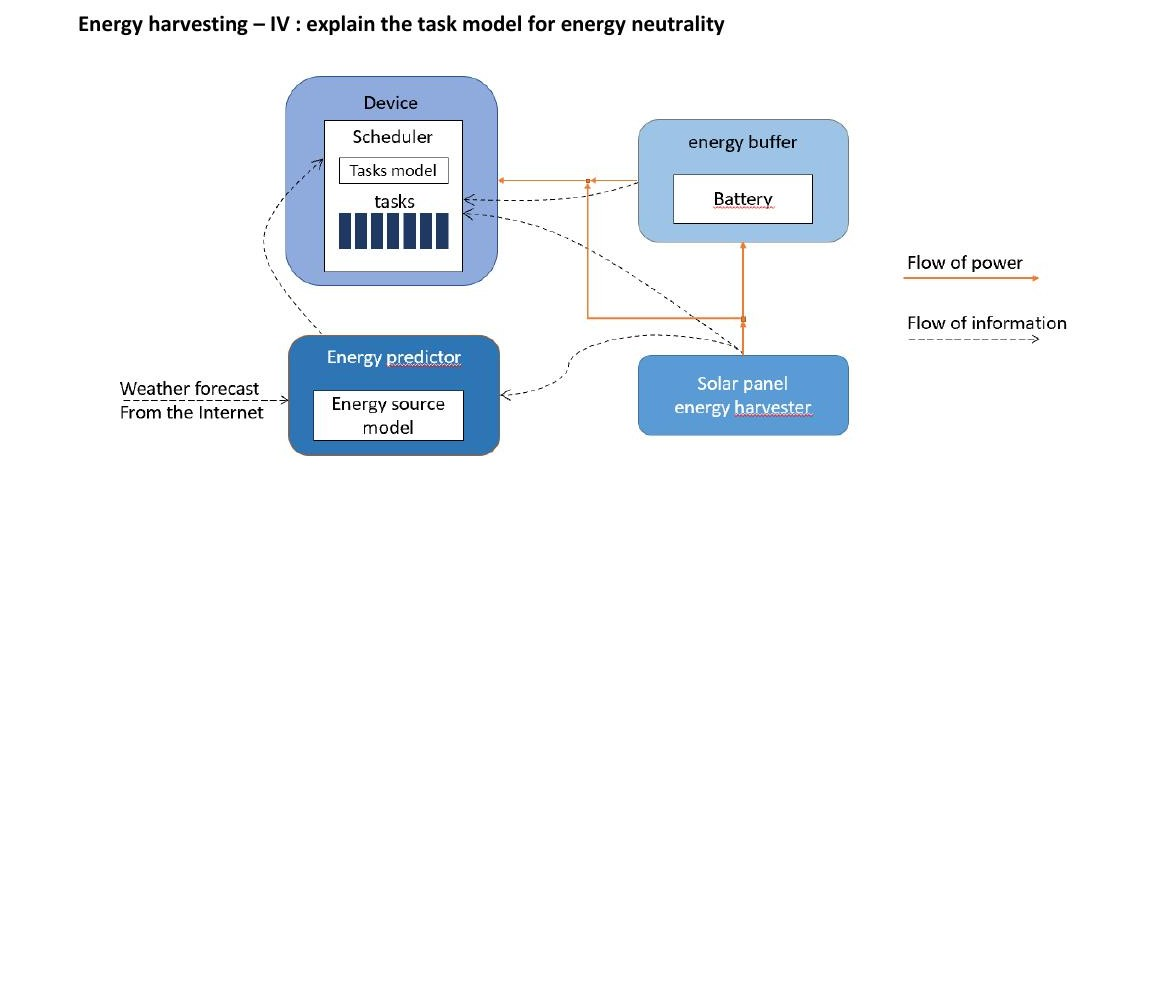
\includegraphics[keepaspectratio]{images/exam-chessa-kansal-taskmodel.jpg}}
\caption{Task model: lo Scheduler pianifica i task in base al Tasks
model (energia per task) e alle previsioni energetiche dell'Energy
predictor (alimentato da weather forecast e da un Solar panel harvester
collegato alla Battery).}
\end{figure}

Lo schema espande il sistema Kansal con il dettaglio del \textbf{task
model}. Rispetto allo schema III, qui è esplicitato il ruolo delle
previsioni meteorologiche esterne.

\textbf{Componenti}:

\begin{itemize}
\tightlist
\item
  \textbf{Tasks model}: specifica il costo energetico di ogni task (es.
  campionamento = X mJ, trasmissione = Y mJ). Il Scheduler usa questo
  modello per stimare quanta energia consumerà ogni operazione.
\item
  \textbf{Scheduler}: dato il livello attuale della batteria e la
  previsione di energia futura, decide:

  \begin{itemize}
  \tightlist
  \item
    Quali task eseguire nel prossimo periodo.
  \item
    A quale frequenza/duty cycle eseguirli.
  \item
    Obiettivo: massimizzare la qualità del servizio senza violare
    l'energy neutrality.
  \end{itemize}
\item
  \textbf{Energy predictor + Energy source model}: riceve dati dal
  weather forecast (Internet) e dalle misurazioni del pannello solare
  per costruire un modello predittivo della produzione energetica
  futura.
\item
  \textbf{Solar panel energy harvester → Battery}: flusso di potenza
  fisico (linea arancione); informazioni di stato (linea tratteggiata)
  comunicano il livello di carica allo Scheduler.
\end{itemize}

\textbf{Flusso informativo} (linee tratteggiate): - Weather forecast →
Energy source model → Energy predictor → Scheduler - Battery state →
Scheduler (per decisioni in tempo reale) - Tasks model → Scheduler (per
la stima del costo)

\begin{calloutnote}{Riferimento}

{[}{[}Lezione 28 - Kansal Problem e Energy Neutrality{]}{]}

\end{calloutnote}

\begin{center}\rule{0.5\linewidth}{0.5pt}\end{center}

\section{Directed Diffusion}\label{directed-diffusion}

\begin{figure}
\centering
\pandocbounded{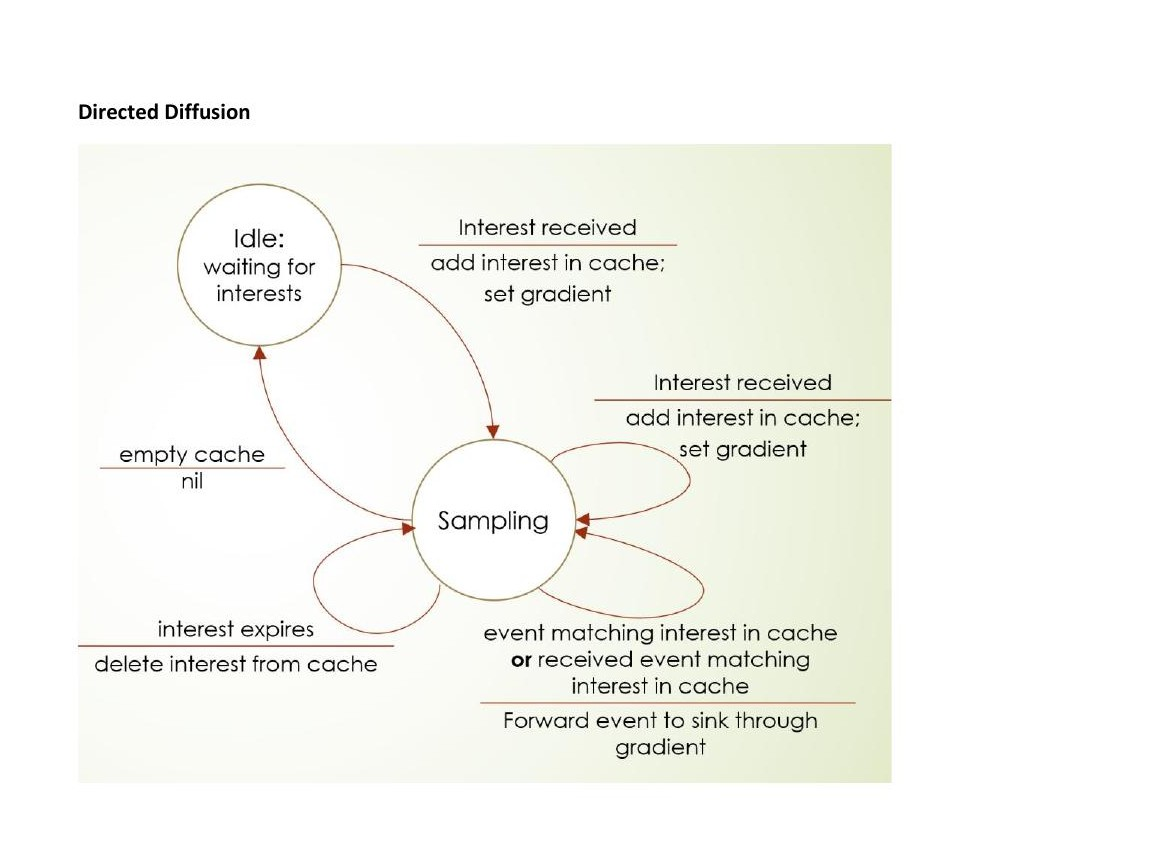
\includegraphics[keepaspectratio]{images/exam-chessa-directed-diffusion.jpg}}
\caption{Macchina a stati della Directed Diffusion: il nodo è Idle
finché non riceve un interest; passa a Sampling e forward gli eventi
corrispondenti verso il sink; torna Idle all'expire dell'interest.}
\end{figure}

\textbf{Directed Diffusion} è un protocollo di routing
\textbf{data-centric} per WSN, in cui i dati vengono nominati con coppie
attributo-valore (non con indirizzi di rete).

\textbf{Fasi principali}:

\begin{enumerate}
\def\labelenumi{\arabic{enumi}.}
\item
  \textbf{Interest propagation}: il sink diffonde in broadcast un
  \textbf{interest} (query) che descrive il tipo di dati desiderati (es.
  \texttt{type=temperature,\ area=sector-A,\ interval=30s}). Ogni nodo
  intermedio memorizza l'interest nella propria \textbf{interest cache}
  e imposta un \textbf{gradiente} verso il nodo da cui ha ricevuto
  l'interest (direzione verso il sink).
\item
  \textbf{Sampling} (stato attivo): un nodo che ha interest in cache e
  rileva dati corrispondenti (o riceve eventi corrispondenti da nodi
  vicini) li \textbf{forwarda verso il sink attraverso il gradiente}
  impostato.
\item
  \textbf{Expire e ritorno a Idle}: quando l'interest scade
  (\texttt{interest\ expires}), il nodo lo elimina dalla cache e torna
  allo stato Idle in attesa di nuovi interest.
\end{enumerate}

\textbf{La macchina a stati del nodo}: - \textbf{Idle} (waiting for
interests): radio in ascolto, nessun sampling attivo. -
\textbf{Sampling}: il nodo è in fase di rilevamento e forwarding. -
Transizione Idle → Sampling: all'arrivo di un
\texttt{interest\ received} → cache interest, set gradient. -
Transizione Sampling → Idle: \texttt{interest\ expires} → delete from
cache. - Permanenza in Sampling: se arriva un nuovo interest → aggiorna
cache e gradiente. - Evento in Sampling: se
\texttt{event\ matching\ interest\ in\ cache} → forward al sink tramite
gradiente.

\textbf{Reinforcement}: il sink può rinforzare il percorso migliore
inviando un interest più frequente lungo il path ottimale, aumentando la
frequenza di ricezione dati da quel percorso.

\begin{center}\rule{0.5\linewidth}{0.5pt}\end{center}

\section{GPSR - I (Greedy Forwarding e
Void)}\label{gpsr---i-greedy-forwarding-e-void}

\begin{figure}
\centering
\pandocbounded{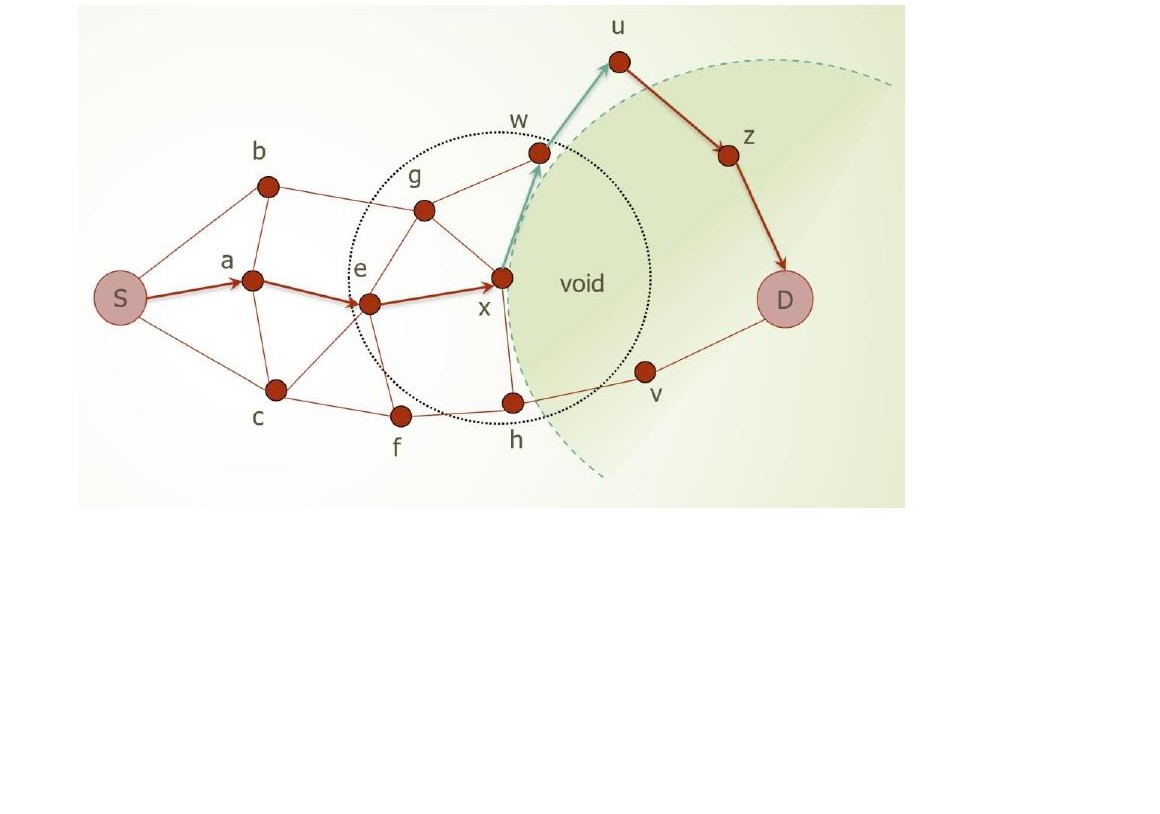
\includegraphics[keepaspectratio]{images/exam-chessa-gpsr-greedy.jpg}}
\caption{GPSR greedy: S forwarda verso x (più vicino a D); x incontra un
void (nessun vicino è più vicino a D di x stesso) → attiva il perimeter
routing attorno al void per raggiungere D.}
\end{figure}

\textbf{GPSR} (\emph{Greedy Perimeter Stateless Routing}) è un
protocollo di routing geografico per WSN che usa le posizioni fisiche
dei nodi. Ogni nodo conosce la propria posizione GPS e quella dei propri
vicini immediati.

\textbf{Greedy Forwarding}: - Ogni nodo forward il pacchetto al vicino
\textbf{più vicino geograficamente alla destinazione D}. - Esempio: S →
a → e → x, perché in ogni hop si seleziona il vicino con distanza minima
da D. - Efficiente quando esiste sempre un vicino più vicino alla
destinazione.

\textbf{Il problema del Void}: - Un nodo \(x\) si trova in un
\textbf{void} quando nessuno dei suoi vicini è geograficamente più
vicino a D di \(x\) stesso. - Il greedy routing si blocca in un void. -
Nell'immagine: \(x\) è circondato da un void (area verde chiaro) →
nessun vicino è più vicino a D.

\textbf{Soluzione --- Perimeter Routing}: - Quando si incontra un void,
GPSR passa al \textbf{perimeter routing} (face routing). - Il nodo \(x\)
inizia a navigare il confine del void usando la \textbf{right-hand rule}
sul grafo planare. - Il perimeter routing termina quando si raggiunge un
nodo più vicino a D rispetto al punto in cui si è entrati nel void. -
Poi si torna al greedy forwarding.

\begin{center}\rule{0.5\linewidth}{0.5pt}\end{center}

\section{GPSR - II (Perimeter Routing / Face
Traversal)}\label{gpsr---ii-perimeter-routing-face-traversal}

\begin{figure}
\centering
\pandocbounded{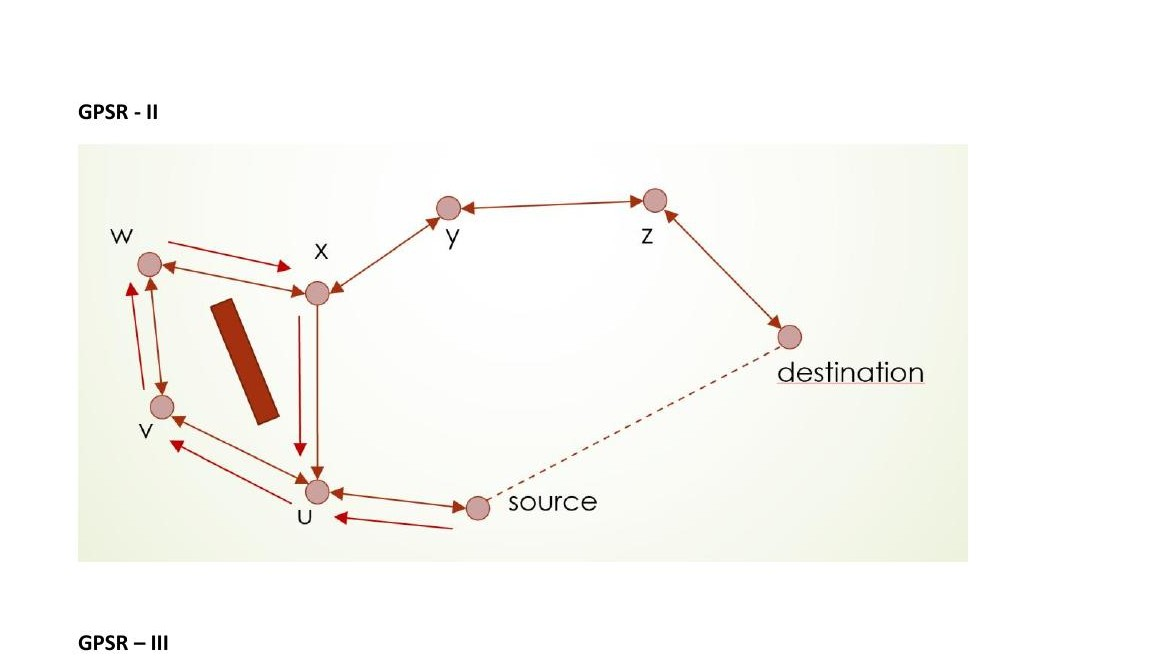
\includegraphics[keepaspectratio]{images/exam-chessa-gpsr-perimeter.jpg}}
\caption{Perimeter routing: il pacchetto naviga il confine del void
(obstacle rettangolare) passando per w→x→y→z→destination, con alcuni
nodi che rimandano indietro il pacchetto durante la face traversal.}
\end{figure}

Il \textbf{perimeter routing} di GPSR è basato sulla \textbf{right-hand
rule} applicata a un grafo planare:

\textbf{Right-hand rule}: muovendo verso il prossimo hop, gira sempre
verso l'arco più a destra disponibile rispetto alla direzione di
provenienza. Questo garantisce di attraversare ogni faccia del grafo
esattamente una volta.

\textbf{Nell'esempio}: - Il pacchetto entra in modalità perimeter a x
(che è nel void). - Naviga seguendo la right-hand rule: x → y → z →
destination, con possibili rimbalzi tra nodi adiacenti. - L'obstacle
rettangolare (area rossa) rappresenta la zona senza nodi. - Le frecce
mostrano il percorso che circumnaviga l'obstacle. - Quando si raggiunge
un nodo (y, z) con distanza da D minore di quella del nodo di ingresso
nel perimeter (x), si torna al greedy forwarding.

\textbf{Importante}: il perimeter routing funziona solo su un
\textbf{grafo planare} (senza archi che si incrociano). Per questo GPSR
richiede una fase di planarizzazione del grafo.

\begin{center}\rule{0.5\linewidth}{0.5pt}\end{center}

\section{GPSR - III (Planarizzazione: Gabriel Graph e
RNG)}\label{gpsr---iii-planarizzazione-gabriel-graph-e-rng}

\begin{figure}
\centering
\pandocbounded{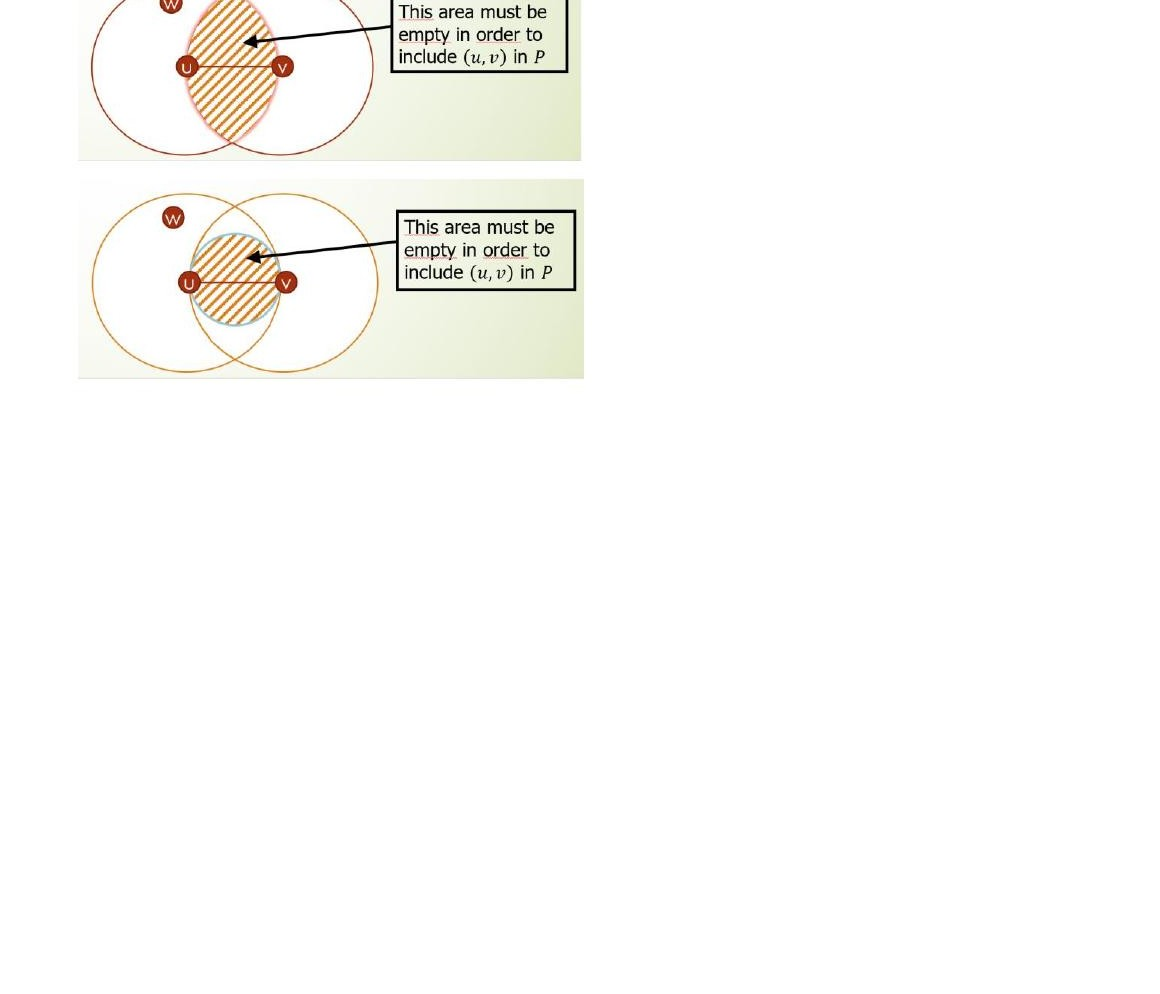
\includegraphics[keepaspectratio]{images/exam-chessa-gpsr-planarization.jpg}}
\caption{Planarizzazione del grafo: GG (sopra) e RNG (sotto). Un arco
(u,v) è incluso solo se nessun nodo w cade nell'area tratteggiata
(cerchio per GG, lente per RNG).}
\end{figure}

Per applicare il face routing, GPSR ha bisogno di un \textbf{grafo
planare} (senza archi incrociati). Due algoritmi di planarizzazione
distribuita sono usati:

\textbf{Gabriel Graph (GG)}: - Un arco \((u, v)\) è incluso nel GG se e
solo se il \textbf{cerchio} con diametro \(\overline{uv}\) non contiene
nessun altro nodo \(w\). - Formalmente: \(|uw|^2 + |vw|^2 > |uv|^2\) per
ogni \(w\) vicino di entrambi \(u\) e \(v\). - Nel diagramma superiore:
il cerchio (area tratteggiata) deve essere vuoto per includere l'arco.

\textbf{Relative Neighborhood Graph (RNG)}: - Un arco \((u, v)\) è
incluso se la \textbf{regione a lente} (intersezione dei cerchi di
raggio \(|uv|\) centrati in \(u\) e \(v\)) non contiene nessun altro
nodo \(w\). - Formalmente: \(|uw| < |uv|\) e \(|vw| < |uv|\) → \(w\) è
nella lente → l'arco viene eliminato. - Nel diagramma inferiore: la
lente tratteggiata deve essere vuota.

\textbf{RNG ⊆ GG}: l'RNG è più sparso (meno archi) del GG, perché la
lente è più piccola del cerchio. Entrambi producono grafi planari su cui
il face routing funziona correttamente.

\textbf{Distribuzione}: ogni nodo può calcolare localmente quali archi
includere o escludere, consultando solo i propri vicini diretti. Non è
richiesto stato globale.

\begin{center}\rule{0.5\linewidth}{0.5pt}\end{center}

\begin{calloutnote}{Riepilogo degli argomenti}

{\def\LTcaptype{none} % do not increment counter
\begin{longtable}[]{@{}
  >{\raggedright\arraybackslash}p{(\linewidth - 2\tabcolsep) * \real{0.3333}}
  >{\raggedright\arraybackslash}p{(\linewidth - 2\tabcolsep) * \real{0.6667}}@{}}
\toprule\noalign{}
\begin{minipage}[b]{\linewidth}\raggedright
Argomento
\end{minipage} & \begin{minipage}[b]{\linewidth}\raggedright
Lezione di riferimento
\end{minipage} \\
\midrule\noalign{}
\endhead
\bottomrule\noalign{}
\endlastfoot
Interoperabilità, vertical silos, vendor lock-in & {[}{[}Lezione 3 -
Interoperabilità e Standard{]}{]} \\
IoT Security, ITU-T Y.2066 & {[}{[}Lezione 3 - Interoperabilità e
Standard{]}{]} \\
MQTT pub/sub, topic, QoS 0/1/2 & {[}{[}Lezione 4 - MQTT Part 1{]}{]} \\
MQTT sessioni, retained, last will, keepalive & {[}{[}Lezione 8 - MQTT
Part 2{]}{]} \\
ZigBee join, stack, topologie, indirizzamento & {[}{[}Lezione 9 - The
ZigBee Standard Part 1{]}{]} \\
ZigBee application layer, cluster, binding & {[}{[}Lezione 12 -
Application Layer of ZigBee{]}{]} \\
Duty cycle, embedded programming Arduino/TinyOS & {[}{[}Lezione 23 -
Embedded Programming e Arduino{]}{]} \\
SMAC, BMAC, X-MAC & {[}{[}Lezione 17 - MAC Protocols{]}{]} \\
IEEE 802.15.4 superframe, indirect transfer & {[}{[}Lezione 18 - The
IEEE 802.15.4 Standard{]}{]} \\
Energy harvesting, architetture, fonti & {[}{[}Lezione 24 - Energy
Harvesting IoT{]}{]} \\
Kansal, task model, energy neutrality & {[}{[}Lezione 28 - Kansal
Problem e Energy Neutrality{]}{]} \\
\end{longtable}
}

\end{calloutnote}

\newpage

\backmatter
\end{document}
